%MIT OpenCourseWare: https://ocw.mit.edu
%RES.18-011 Algebra I Student Notes, Fall 2021
%License: Creative Commons BY-NC-SA 
%For information about citing these materials or our Terms of Use, visit: https://ocw.mit.edu/terms.

\documentclass[a4paper]{article}
\usepackage{jakin2} % style
\usepackage{asymptote}

\title{18.701: Algebra 1}
\author{Jakin Ng, Sanjana Das, and Ethan Yang}
\date{Fall 2021}

% \rhead{\rightmark}
\rhead{}
\begin{document}
\maketitle
\tableofcontents
\pagebreak

\lhead{Lecture 1: Groups}
%MIT OpenCourseWare: https://ocw.mit.edu
%RES.18-011 Algebra I Student Notes, Fall 2021
%License: Creative Commons BY-NC-SA 
%For information about citing these materials or our Terms of Use, visit: https://ocw.mit.edu/terms.

\section{Groups}
\subsection{Introduction}
The lecturer is \textbf{Davesh Maulik}. These notes are taken by \textbf{Jakin Ng}, \textbf{Sanjana Das}, and \textbf{Ethan Yang}. Here is some basic information about the class:
\begin{itemize}
    \item The text used in this class will be the 3rd edition of \textbf{Algebra}, by Artin. 

    \item The course website is found on \textbf{Canvas}, and the problem sets will be submitted on \textbf{Gradescope}. 
    
    \item The problem sets will be due every Tuesday at midnight.
\end{itemize}

Throughout this semester, we will discuss the fundamentals of \emph{linear algebra} and \emph{group theory}, which is the study of symmetries. In this class, we will mostly study groups derived from geometric objects or vector spaces, but in the next course, 18.702\footnote{Algebra 2}, more exotic groups will be studied. 

As a review of basic linear algebra, let's review invertible matrices.

\begin{definition}
An $n \by n$ matrix\footnote{An array of numbers (or some other type of object) with $n$ rows and $n$ columns} $A$ is invertible if there exists some other matrix $A^{-1}$ such that $AA^{-1} = A^{-1}A = I$, the $n \by n$ identity matrix. Equivalently, $A$ is invertible if and only if the determinant $\det(A) \neq 0.$  
\end{definition}

\begin{example}[$n = 2$]
Let $A = \begin{pmatrix}a & b \\ c & d\end{pmatrix}$ be a $2 \by 2$ matrix. Then its inverse $A^{-1}$ is $\frac{1}{ad-bc}\begin{pmatrix}
d & -b \\ -c & a
\end{pmatrix}$.
\end{example}

\begin{example}[$GL_n(\RR)$]
A main example that will guide our discussion of groups\footnote{The concept of a \emph{group} will be fleshed out later in this lecture} is the \textbf{general linear group}, $GL_n(\RR),$ which is the group of $n \by n$ invertible real matrices. 
\end{example}

Throughout the course, we will be returning to this example to illustrate various concepts that we learn about.

\subsection{Laws of Composition}
With our example in mind, let's start.
\begin{qq}
How can we generalize the nice properties of matrices and matrix multiplication in a useful way?
\end{qq}

Given two matrices $A, B \in GL_n(\RR),$ there is an operation combining them, in particular \emph{matrix multiplication}, which returns a matrix $AB \in GL_n(\RR)$.\footnote{Since the determinant is multiplicative, $\det(AB) = \det(A)\det(B),$ which is nonzero.} The matrices under matrix multiplication satisfy several properties:
\begin{itemize}
    \item \textbf{Noncommutativity.} Matrix multiplication is noncommutative, which means that $AB$ is not necessarily the same matrix as $BA.$ So the order that they are listed in \emph{does} matter.
    \item \textbf{Associativity.} This means that $(AB)C = A(BC),$ which means that the matrices to be multiplied can be grouped together in different configurations. As a result, we can omit parentheses when writing the product of more than two matrices.
    
    \item \textbf{Inverse.} The product of two invertible matrices is also invertible. In particular, 
    \[
    (AB)^{-1} = B^{-1}A^{-1}.
    \]
\end{itemize}

Another way to think of matrices is as an \emph{operation} on a different space. Given a matrix $A \in GL_n(\RR),$ a function or transformation on $\RR^n$\footnote{Vectors with $n$ entries which are real numbers.} can be associated to it, namely 
\begin{align*}
    T_A: \RR^n &\rto \RR^n \\
    \vvv = (x_1, \cdots, x_n) &\mto A\vvv \footnotemark.
\end{align*}
\footnotetext{The notation $A\vvv$ refers to the matrix product of $A$ and $\vvv$, considered as $n \by n$ and $n \by 1$ matrices.}

Since $A\vvv$ is the matrix product, we notice that $T_{AB}(\vvv) = T_A(T_B(\vvv)),$ and so matrix multiplication is the same as function composition. 

With this motivation, we can define the notion of a group. 
\begin{definition}[Group]
A \textbf{group} is a set $G$ with a composition (or product) law 
\begin{align*}
    G \by G &\rto G \\
    (a, b) &\mto a\cdot b\footnotemark %\footnote{Also denoted $ab$}
\end{align*}
\footnotetext{Also denoted $ab$}
fulfilling the following conditions:
\begin{itemize}
    \item \textbf{Identity.} There exists some element $e \in G$ such that $a \cdot e = e \cdot a = a$
    \item \textbf{Inverse.} For all $a \in G,$ there exists $b \in G$, denoted $a^{-1}$, such that $a \cdot b = b \cdot a = e$. 
    
    \item \textbf{Associative.} For $a, b, c \in G,$
    \[
    (ab)c = a(bc).
    \]
\end{itemize}
\end{definition}
In the definition, both the first and second conditions automatically give us a unique inverse and identity. For example, if $e$ and $e'$ both satisfy property 1, then $e\cdot e' = e = e',$ so they must be the same element. A similar argument holds for inverses. 

Why does associativity matter? It allows us to define the product $g_1 \cdot g_2\cdot  \cdots \cdot g_n$ without the parentheses indicating which groupings they're multiplied in. 

\begin{definition}
Let $g$ taken to the power $n$ be the element $g^n = \underbrace{g\cdot \cdots \cdot g}_{n \text{ times}}$ for $n > 0,$ $g^n = \underbrace{g^{-1}\cdot \cdots \cdot g^{-1}}_{n \text{ times}}$ for $n < 0,$ and $e$ for $n = 0.$
\end{definition}

\begin{example}
Some common groups include:

\begin{center}
\begin{tabular}{ c c c c }
 Group & Composition Law & Identity & Inverse \\ 
 $GL_n(\RR)$\footnote{The general linear group} & matrix multiplication & $I_n$ & $A \mapsto A^{-1}$ \\  
 $\ZZ$\footnote{The integers under addition} & + & 0 & $n \mapsto -n$ \\
 $\CC^{\by} = \CC\setminus \{0\}$\footnote{The complex numbers (except 0) under multiplication} & $\by$ & 1 & $z \mapsto \frac{1}{z}$
\end{tabular}
\end{center}

\end{example}

For the last two groups, there is additional structure: the composition law is \emph{commutative}. This motivates the following definition.
\begin{definition}
A group $G$ is \textbf{abelian} if $a \cdot b = b \cdot a$ for all $a, b \in G.$ Otherwise, $G$ is called \textbf{nonabelian}.
\end{definition}

Often, the composition law in an abelian group is denoted $+$ instead of $\cdot.$


\subsection{Permutation and Symmetric Groups}
Now, we will look at an extended example of another family of nonabelian groups.

\begin{definition}
Given a set $S,$ a \textbf{permutation} of $S$ is a \emph{bijection}\footnote{A function $f: A \rto B$ is a bijection if for all $y \in B$, there exists a unique $x \in A$ such that $f(x) = y$. Equivalently, it must be one-to-one and onto.} $p: S \rto S$.
\end{definition}

\begin{definition}
Let $\text{Perm}(S)$ be the set of permutations of $S$. 
\end{definition}

In fact, $\text{Perm}(S)$ is a group, where the product rule is function composition.\footnote{We can check that the composition of two bijections $p \circ q$ is also a bijection.}
\begin{itemize}
    \item \textbf{Identity.} The identity function $e: x \mto x$ is is the identity element of the group.
    
    \item \textbf{Inverse.} Because $p$ is a bijection, it is invertible. Let $p^{-1}(x)$ be the unique $y \in S$ such that $p(y) = x.$
    
    \item \textbf{Associativity.} Function composition is always associative.
\end{itemize}

Like groups of matrices, $\text{Perm}(S)$ is a group coming from a set of \emph{transformations} acting on some object; in this case, $S$. 

\begin{definition}
When $S = \{1, 2, \cdots, n\},$ the permutation group $\text{Perm}(S)$ is called the \textbf{symmetric group}, denoted $S_n.$
\end{definition}

\begin{definition}
For a group $G,$ the number of elements in the set $G,$ $|G|,$ is called the \textbf{order} of the group $G,$ denoted $|G|$ or $\ord(G).$
\end{definition}

The order of the symmetric group is $|S_n| = n!$\footnote{The number of permutations of the numbers 1 through $n$ is $n!$ --- there are $n$ possibilities for where 1 maps to, and then $n-1$ for where 2 maps to, and so on to get $n(n-1)\cdots (2)(1) = n!$} so the symmetric group $S_n$ is a \emph{finite} group. 

For $n=6,$ consider the two permutations $p$ and $q$
\begin{center}
    \begin{tabular}{c|c c c c c c}
     $i$ & 1 & 2 & 3 & 4 & 5 & 6 \\
     \hline 
     $p(i)$ & 2 & 4 & 5 & 1 & 3 & 6
\end{tabular}
\end{center}
\begin{center}
    \begin{tabular}{c|c c c c c c}
     $i$ & 1 & 2 & 3 & 4 & 5 & 6 \\
     \hline 
     $q(i)$ & 3 & 4 & 5 & 6 & 1 & 2
\end{tabular},
\end{center}
where the upper number is mapped to the lower number. 

We can also write these in \textbf{cycle notation}, which is a shorthand way of describing a permutation that does not affect what the permutation actually is. In cycle notation, each group of parentheses describes a cycle, where the number is mapped to the following number, and it wraps around. 
\begin{example}[Cycle notation]
In cycle notation, $p$ is written as $(124)(35),$ where the 6 is omitted. In the first cycle, 1 maps to 2, 2 maps to 4, and 4 maps to 1, and in the second cycle, 3 maps to 5 and 5 maps back to 3.\footnote{In fact, we say that $p$ has \emph{cycle type} $(3, 2),$ which is the lengths of each cycle.} 
\end{example}

Similarly, $q$ is written as $(135)(246).$\footnote{It has cycle type $(3, 3).$} In cycle notation, it is clear that there are multiple ways to write or represent the same permutation. For example, $p$ could have been written as $(241)(53)$ instead, but it represents the \emph{same} element $p \in S_6.$

Cycle notation allows us to more easily invert or compose two permutations; we simply have to follow where each number maps to. 

\begin{example}[Inversion]
The inverse $p^{-1}$ flips the rows of the table:
\begin{center}
    \begin{tabular}{c|c c c c c c}
     $i$ & 2 & 4 & 5 & 1 & 3 & 6 \\
     \hline 
     $p(i)$ & 1 & 2 & 3 & 4 & 5 & 6 
\end{tabular}
\end{center}

In cycle notation, it reverses the cycles, since each number should be mapped under $p^{-1}$ to the number that maps to it under $p$:
\[
p^{-1} = (421)(53) = (142)(35).
\]
\end{example}

\begin{example}[Composition]
The composition is
\[
q \circ p = (143)(26).
\]
Under $p,$ 1 maps to 2, which maps to 4 under $q$, and so 1 maps to 4 under $q \circ p.$\footnote{Remember that the rightmost permutation is applied first, and then the leftmost, and not the other way around, due to the notation used for function composition.} Similarly, 4 maps to 3 and 3 maps back to 1, which gives us the first cycle. The second cycle is similar.  
\end{example}

\begin{example}[Conjugation]
Another example of composition is
\[
p^{-1} \circ q \circ p = (126)(345).
\]
This is also known as \emph{conjugation} of $q$ by $p.$\footnote{Notice that under conjugation, $q$ retains its cycle type $(3, 3).$ In fact, this is true for conjugation of any element by any other element!}
\end{example}

\subsection{Examples of Symmetric Groups}
For $n \geq 3,$ $S_n$ is always non-abelian. Let's consider $S_n$ for small $n \leq 3.$
\begin{example}[$S_1$]
In this case, $S_1$ only has one element, the identity element, and so it is $\{e\},$ the \emph{trivial group.}
\end{example}

\begin{example}[$S_2$]
For $n = 2,$ the only possibilities are the identity permutation $e$ and the transposition $(12).$ Then $S_2 = \{e, (12)\};$ it has order 2.
\end{example}

Once $n$ gets larger, the symmetric group becomes more interesting. 
\begin{example}[$S_3$]
The symmetric group on three elements is of order $3! = 6.$ It must contain the identity $e.$ It can also contain $x = (123).$ Then we also get the element $x^2 = (132)$, but \[\boxed{x^3 = e.}\] Higher powers are just $x^4 = x, x^5 = x^2,$ and so on. Now, we can introduce $y = (12),$ which is its own inverse, and so \[\boxed{y^2 = e}.\] Taking products gives $xy = (13)$ and $x^2y = (23).$ So we have all six elements of $S_3$:
\[
S_3 = \{e, (123), (132), (12), (13), (23)\}.
\]

In fact, $yx = (23) = x^2y,$ so taking products in the other order does not provide any new elements. The relation
\[
\boxed{yx = x^2y}
\]
holds. In particular, using the boxed relations, we can compute \emph{any} crazy combination of $x$ and $y$ and reduce it to one of the elements we listed. For example, $xyx^{-1}y = xyx^2y = xyyx = xy^2x = x^2.$ 
\end{example}

\newpage

\lhead{Lecture 2: Subgroups and Cyclic Groups}
\setcounter{section}{1}
%MIT OpenCourseWare: https://ocw.mit.edu
%RES.18-011 Algebra I Student Notes, Fall 2021
%License: Creative Commons BY-NC-SA 
%For information about citing these materials or our Terms of Use, visit: https://ocw.mit.edu/terms.

\section{Subgroups and Cyclic Groups}
\subsection{Review}
Last time, we discussed the concept of a group, as well as examples of groups. In particular, a group is a set $G$ with an associative composition law $G \by G \rto G$ that has an identity as well inverses for each element with respect to the composition law $\by.$ 

Our guiding example was that of the group of invertible $n \by n$ matrices, known as the \textbf{general linear group} ($GL_n(\RR)$ or $GL_n(\CC),$ for matrices over $\RR$ and $\CC,$ respectively.) 
\begin{example}
Let $GL_n(\RR)$ be the group of $n \by n$ invertible real matrices. 
\begin{itemize}
    \item \textbf{Associativity.} Matrix multiplication is associative; that is, $(AB)C = A(BC)$, and so when writing a product consisting of more than two matrices, it is not necessary to put in parentheses. 
    \item \textbf{Identity.} The $n \by n$ identity matrix is $I_n = \begin{pmatrix}1 & \cdots & 0 \\ \vdots & \ddots & \vdots \\ 0 & \cdots & 1\end{pmatrix}$, which is the matrix with 1s along the diagonal and 0s everywhere else. It satisfies the property that $AI = IA = A$ for all $n \by n$ matrices $A$. 
    \item \textbf{Inverse.} By the invertibility condition of $GL_n,$ every matrix $A \in GL_n(\RR)$ has an inverse matrix $A^{-1}$ such that $AA^{-1} = A^{-1}A = I_n.$
\end{itemize}
\end{example}
Furthermore, each of these matrices can be seen as a transformation from $\RR^n \rto \RR^n$, taking each vector $\vec{v}$ to $A\vec{v}.$ That is, there is a bijective correspondence between matrices $A$ and invertible transformations $T_A: \RR^n \rto \RR^n$ taking $T_A(\vec{v}) = A\vec{v}.$

Another example that showed up was the integers under addition. 

\begin{example}
The integers $\ZZ$ with the composition law $+$ form a group. Addition is associative. Also, $0 \in \ZZ$ is the additive identity, and $-a \in \ZZ$ is the inverse of any integer $a.$
\end{example}
On the other hand, the natural numbers $\NN$ under addition would \emph{not} form a group, because the invertibility condition would be violated.

Lastly, we looked at the symmetric group $S_n.$ 

\begin{example}
The \textbf{symmetric group} $S_n$ is the permutation group of $\{1, \cdots, n\}.$ 
\end{example}

\subsection{Subgroups}
In fact, understanding $S_n$ is important for group theory as a whole because \emph{any} finite group "sits inside" $S_n$ in a certain way\footnote{This is known as \emph{Cayley's Theorem} and is discussed further in section 7.1 of Artin.}, which we will begin to discuss today.
\begin{qq}
What does it mean for a group to "sit inside" another group?
\end{qq}

If a subset of a group satisfies certain properties, it is known as a \emph{subgroup.}
\begin{definition}
Given a group $(G, \cdot)$, a subset $H \subset G$ is called a \textbf{subgroup} if it satisfies:
\begin{itemize}
    \item \textbf{Closure.} If $h_1, h_2 \in H,$ then $h_1 \cdot h_2 \in H.$
    \item \textbf{Identity.} The identity element $e$ in $G$ is contained in $H.$
    \item \textbf{Inverse.} If $h \in H,$ its inverse $h^{-1}$ is also an element of $H.$
\end{itemize}

As notation, we write $H \leq G$ to denote that $H$ is a subgroup of $G.$
\end{definition}

Essentially, these properties consists solely of the necessary properties for $H$ to also be a group under the same operation $\cdot,$ so that it can be considered a subgroup and not just some arbitrary subset. In particular, any subgroup $H$ will also be a group with the same operation, independent of the larger group $G.$

\begin{example}
The integers form a subgroup of the rationals under addition: $(\ZZ, +) \subset (\QQ, +).$
\end{example}
The rationals are more complicated than the integers, and studying simpler subgroups of a certain group can help with understanding the group structure as a whole.

\begin{example}
The symmetric group $S_3$ has a three-element subgroup $\{e, (123), (132)\} = \{e, x, x^2\}.$
\end{example}

However, the natural numbers $\NN = \{0, 1, 2, \cdots \} \subset (\ZZ, +)$ are \textbf{not} a subgroup of the integers, since not every element has an inverse.

\begin{example}
The matrices with determinant 1, called the \textbf{special linear group}, form a subgroup of invertible matrices: $SL_n(\RR) \subset GL_n(\RR).$
\end{example}
The special linear group is closed under matrix multiplication because $\det(AB) = \det(A)\det(B).$ 

\subsection{Subgroups of the Integers}
The integers $(\ZZ, +)$ have particularly nice subgroups. 
\begin{theorem}\label{subgroup of z}
The subgroups of $(\ZZ, +)$ are $\{0\}, \ZZ, 2\ZZ, \cdots.$\footnote{Where $n \in \ZZ,$ $n\ZZ$ consists of the multiples of $n,$ $\{nx: x \in \ZZ\}$.}
\end{theorem}

This theorem demonstrates that the condition that a subset $H$ of a group be a subgroup is quite strong, and requires quite a bit of structure from $H.$

\begin{proof}
First, $n\ZZ$ is in fact a subgroup.
\begin{itemize}
    \item \textbf{Closure.} For $na, nb \in n\ZZ,$ $na + nb = n(a + b).$
    \item \textbf{Identity.} The additive identity is in $n\ZZ$ because $0 = n \cdot 0.$
    
    \item \textbf{Inverse.} For $na \in n\ZZ,$ its inverse $-na = n(-a)$ is also in $n\ZZ.$
\end{itemize}

Now, suppose $S \subset \ZZ$ is a subgroup. Then clearly the identity $0$ is an element of $S.$ If there are no more elements in $S,$ then $S = \{0\}$ and the proof is complete. Otherwise, pick some nonzero $h \in S.$ Without loss of generality, we assume that $h > 0$ (otherwise, since $-h \in S$ as well by the invertibility condition, take $-h$ instead of $h.$) Thus, $S$ contains at least one positive integer; let $a$ be the smallest positive integer in $S.$ 

Then we claim that $S = a\ZZ.$ If $a \in S,$ then $a + a = 2a \in S$ by closure, which implies that $2a + a = 3a \in S,$ and so on. Similarly, $-a \in S$ by inverses, and $-a + (-a) = -2a \in S,$ and so on, which implies that $a \ZZ \subset S.$ 

Now, take any $n \in S.$ By the Euclidean algorithm, $n = aq + r$ for some $0 \leq r < a.$ From the subgroup properties, $n - aq  = r\in S$ as well. Since $a$ is the smallest positive integer in $S,$ if $r > 0,$ there would be a contradiction, so $r = 0.$ Thus, $n = aq,$ which is an element of $a\ZZ.$ Therefore, $S \subset a\ZZ.$ 

From these two inclusions, $S = a\ZZ$ and the proof is complete.
\end{proof}

\begin{corollary}
Given $a, b \in \ZZ,$ consider $S = \{ai + bj: i, j \in \ZZ\}.$ The subset $S$ satisfies all the subgroup conditions, so by Theorem \ref{subgroup of z}, there is some $d$ such that $S = d\ZZ.$ In fact, $d = \text{gcd}(a, b).$
\end{corollary}
\begin{proof}
Let $e = \text{gcd}(a, b).$ Since $a \in S$, $a = dk$ and $b = d\ell$ for some $k, \ell.$ Since the $d$ from before divides $a$ and $b$, it must also divide $e,$ by definition of the greatest common divisor. Also, since $d \in S,$ by the definition of $S,$ $d = ar + bs$ for some $r$ and $b.$ Since $e$ divides $a$ and $b,$ $e$ divides both $ar$ and $bs$ and therefore $d.$ 

Thus, $d$ divides $e,$ and $e$ divides $d,$ implying that $e = d.$ So $S = \text{gcd}(a, b) \ZZ.$
\end{proof}
 
 In particular, we have showed that $\text{gcd}(a, b)$ can always be written in the form $ar + bs$ for some $r, s$.

\subsection{Cyclic Groups}
Now, let's discuss a very important type of subgroup that connects back to the work we did with $(\ZZ, +).$

\begin{definition}
Let $G$ be a group, and take $g \in G.$ Let the \textbf{cyclic subgroup generated by $g$} be \[
\langle g \rangle \coloneqq\footnote{The $\coloneqq$ symbol is usually used by mathematicians to mean "is defined to be." Other people may use $\equiv$ for the same purpose.} \{\cdots g^{-2}, g^{-1}, g^0=e, g^1, g^2, \cdots\} \leq G.
\]
\end{definition}

Since $g^a \cdot g^b = g^{a + b},$ the exponents of the elements of a cyclic subgroup will have a related group structure to $(\ZZ, +).$

\begin{example}
The identity element generates the trivial subgroup $\{e\} = \langle e \rangle$ of any group $G.$
\end{example}
There are also nontrivial cyclic subgroups.
\begin{example}
In $S_3, $ $\langle (123) \rangle = \{e, (123), (132)\}.$
\end{example}
Evidently, a cyclic subgroup of any finite group must also be finite.
\begin{example}
Let $\CC^{\by}$ be the group of nonzero complex numbers under multiplication. Then $2 \in \CC$ will generate \[\langle 2 \rangle = 
\{\cdots, 1/4, 1/2, 1, 2, 4, \cdots .\}
\]
On the other hand, $i \in \CC$ will generate 
\[
\langle i \rangle = \{1, i, -1, -i\}.
\]
\end{example}

This example shows that a cyclic subgroup of an infinite group can be either infinite or finite.\footnote{Can you work out the cases for which $g \in \CC$ the cyclic subgroup of $\CC^{\by}$ is finite or infinite?}

\begin{qq}
What does a cyclic subgroup look like? Can they be classified?
\end{qq}

\begin{theorem}
Let $S = \{n \in \ZZ: g^n = e\}.$ Then $S$ is a subgroup of $\ZZ,$ so $S = d\ZZ$ or $S = \{0\}$, leading to two cases:
\begin{itemize}
    \item If $S = \{0\},$ then $\langle g \rangle$ is infinite and all the $g^k$ are distinct.
    \item If $S = d\ZZ,$ then $\langle g \rangle = \{e, g, g^2, \cdots, g^{d-1}\} \subset G,$ which is finite.
\end{itemize}
\end{theorem}
\begin{proof}
First, $S$ must be shown to actually be a subgroup of $\ZZ.$
\begin{itemize}
    \item \textbf{Identity.} The identity $0 \in S$ because $g^0 = e.$
    \item \textbf{Closure.} If $a, b \in S,$ then $g^a = g^b = e,$ so $g^{a + b} = g^ag^b = e \cdot e = e,$ so $a + b \in S.$
    \item \textbf{Inverse.} If $a \in S,$ then $g^{-a} = (g^a)^{-1} = e^{-1} = e,$ so $a \in S.$
    
\end{itemize}

Now, consider the first case. If $g^a = g^b$ for any $a, b,$ then multiplying on right by $g^{-b}$ gives $g^a\cdot g^{-b} = g^{a-b} = e.$ Thus, $a - b \in S$, and if $S = \{0\},$ then $a = b.$ So any two powers of $g$ can only be equal if they have the same exponent, and thus all the $g^i$ are distinct and the cyclic group is infinite. 

Consider the second case where $S = d\ZZ.$ Given any $n \in \ZZ,$ $n = dq + r$ for $0 \leq r < d$ by the Euclidean algorithm. Then $g^n = g^{dq} \cdot g^r = g^r,$ which is in $\{e, g, g^2, \cdots, g^{d-1}\}.$
\end{proof}

\begin{definition}
So if $d = 0,$ then $\langle g \rangle$ is infinite; we say that $g$ has \textbf{infinite order.} Otherwise, if $d \neq 0,$ then $|\langle g \rangle| = d$ and $g$ has \textbf{order} $d$.
\end{definition}

It is also possible to consider more than one element $g.$ 
\begin{definition}
Given a subset $T \subset G$, the subgroup generated by $T$ is \[\langle T \rangle \coloneqq \{t_1^{e_1}\cdots t_n^{e_n} \mid t_i \in T, e_i \in \ZZ\}.\] 
% Given a subset $T =\{g_1, g_2, \cdots, \} \subset G$, the subgroup generated by $T$ is 
% \[
% \langle T \rangle \coloneqq \{t_1^{\varepsilon_1}\cdot \cdots \cdot t\}
% \]
\end{definition}

Essentially, $\langle T \rangle$ consists of all the possible products of elements in $T.$ For example, if $T = \{t, n\},$ then \[
\langle T \rangle = \{\cdots, t^2n^{-3}t^4, n^5t^{-1}, \cdots \}.
\]
\begin{definition}
If $\langle T \rangle = G,$ then \textbf{$T$ generates $G.$}\footnote{Given a group $G,$ what is the smallest set that generates it? Try thinking about this with some of the examples we've seen in class!}
\end{definition}

\begin{example}
The set $\{(123), (12)\}$ generates $S_3.$ 
\end{example}
\begin{example}
The invertible matrices $GL_n(\RR)$ are generated by elementary matrices\footnote{The matrices giving row-reduction operations.}.
\end{example}

\newpage

\lhead{Lecture 3: Homomorphisms and Isomorphisms}
\setcounter{section}{2}
%MIT OpenCourseWare: https://ocw.mit.edu
%RES.18-011 Algebra I Student Notes, Fall 2021
%License: Creative Commons BY-NC-SA 
%For information about citing these materials or our Terms of Use, visit: https://ocw.mit.edu/terms.

\section{Homomorphisms and Isomorphisms}
\subsection{Review}
Last time, we discussed subgroups and cyclic groups. A subgroup of a group is essentially a subset of that group that is compatible with the group or multiplicative structure on it. A cyclic subgroup of an element $g$ in a group is essentially the subgroup consisting of all the powers of $g.$
\subsection{Homomorphisms}
Now that we understand a little bit more about groups and their structures, the natural next step is to look at maps \emph{between} groups.
\begin{qq}
How can we understand groups by considering maps between different groups? What kinds of maps can provide useful insight into various groups?
\end{qq}

First, we define a type of map that is compatible with the group structure on both groups.

\begin{definition}
Given groups $G$ and $G'$, a homomorphism between them is a map 
\[
f: G \rto G'
\]
such that:
\begin{itemize}
    \item For all $a, b \in G,$ $f(ab) = f(a)f(b)$.
    \item The identity element is mapped to the identity: $f(e_G) = e_{G'}.$
    \item Inverses are preserved under the mapping: $f(a)^{-1}=f(a^{-1})$ for all $a \in G.$
\end{itemize}
\end{definition}

Essentially, each of these conditions requires that the map preserve the group structure (multiplication, identity, inverse) from the domain $G$ to the codomain $G'$. Either $f$ can be applied to a product, or the product can be taken after $f$ is applied, and it should yield the same element $f(ab) = f(a)f(b).$\footnote{In other words, a homomorphism will \emph{commute} with multiplication in that they can be applied in either order. This results in a commutative diagram.} In fact, only the first condition is really necessary, and implies the second two.\footnote{In some way, this shows that the multiplication is the essential part of the group structure, and the identity and inverse properties are simply there to make sure nothing is able to go wrong with the multiplication.}

\begin{proposition}
If $f(ab) = f(a)f(b)$, then $f(e_G) = e_{G'}$ and $f(a)^{-1} = f(a^{-1})$. 
\end{proposition}
\begin{proof}
For the first part, take $f(e_G \cdot e_G) = f(e_G) = f(e_G) \cdot e_{G'}$ by the definition of $e_{G'}.$ Since $f$ is a homomorphism, this will also be equal to $f(e_G)f(e_G).$ Multiplying on both sides by $f(e_G)^{-1}$\footnote{This must exist by the group property of invertibility.} gives $f(e_G) = e_G'.$

The second part is similar. Take $a \in G.$ Then $f(a)\cdot f(a^{-1}) = f(a \cdot a^{-1}) = f(e_G) = e_G',$ and multiplying on the left by $f(a)^{-1}$ gives $f(a^{-1}) = f(a)^{-1}.$
\end{proof}

\subsection{Examples}
Let's see some examples.
\begin{example}
The determinant $\text{det}: GL_n(\RR) \rto (\RR^{\by}, \by)$ is a homomorphism from invertible matrices to the real numbers under multiplication, since $\det(AB) = \det(A)\det(B).$ 
\end{example}

\begin{example}
The exponential $\text{exp}: (\CC, +) \rto (\CC^{\by}, \by)$ taking $z \rto e^z$ is a homomorphism, since $e^{a+b} = e^a e^b.$
\end{example}
Let the standard basis vectors of $\RR^n$ be $\vec{e}_1 = (1, 0, \cdots, 0)^t, \vec{e}_2 = (0, 1, \cdots, 0)^t,$ and so on, where $\vec{e}_i$ is the vector consisting of a 1 in the $i$th entry and 0s elsewhere.

For a permutation $p \in S_n,$ let $A_p$ be the permutation matrix taking $\vec{e}_i \mto \vec{e}_{p(i)}.$ In particular, the $i$th column of $A_p$ will be $\vec{e}_{p(i)}.$ 

For example, for $p  (123),$ $A_p = \begin{pmatrix} 0 & 0 & 1 \\ 1 & 0 & 0 \\ 0 & 1 & 0 \end{pmatrix}$.

\begin{example}
The mapping
\begin{align*}
\varphi: S_n &\rto GL_n(\RR) \\
p\in S_n &\mto A_p,
\end{align*}
where $A_p$ is the permutation matrix, is a homomorphism. This is because $A_p(A_q(\vec{e}_i)) = A_p(\vec{e}_{q(i)}) = \vec{e}_{p(q(i))},$ and $A_{pq}(\vec{e}_i) = \vec{e}_{pq(i)} = \vec{e}_{p(q(i))},$ which matches, so $A_pA_q = A_{pq}.$
\end{example}

There is also another important homomorphism from $S_n$ to another group.

\begin{example}
Let $\text{sign} = \det \circ \varphi$ take $S_n \rto \RR^{\by}$ by taking the determinant of the permutation matrix. This mapping $\text{sign}$ is also a homomorphism, since $\varphi$ and $\det$ are both homomorphisms. 
\end{example}

In fact, $\text{sign}(p) = \pm 1$. It is always possible to write any permutation as a composition of transpositions\footnote{Permutations that swap two elements and leave all other elements fixed.}: $p = \tau_1\tau_2 \cdots \tau_r$ for transpositions $\tau_i$. The determinant of a transposition matrix is $-1,$ since $\det\begin{pmatrix} 0 & 1 \\ 1 & 0 \end{pmatrix} = -1,$ so $\text{sign}(p) = (-1)^r$ where $r$ is the number of transpositions making up $p.$ In fact, if $p = \tau_1\cdots \tau_r = \tau_1'\cdots\tau_s',$ $r = s$ modulo 2, since the sign homomorphism can be applied on either side. For example, for $S_3,$ $e, (123),$ and $(132)$ all have a sign of $+1,$ while $(12), (13),$ and $(23),$ the transpositions, all have a sign of $-1.$

Notice that $\RR^{\by} = GL_1(\RR),$ since $1 \by 1$ invertible matrices are simply nonzero real numbers. These two examples provide a hint as to why homomorphisms are so useful: matrices/linear mappings and $GL_n$ are generally well-understood, so if there is a homomorphism from a group to $GL_n,$ the knowledge from $GL_n$ can then be used to learn more about that particular group. This idea is the core theme of a branch of math called \textbf{representation theory.}\footnote{These examples actually provides the so-called \emph{permutation representation} and \emph{sign representation} of $S_n$.}

\begin{example}\label{fx example}
For any $G$ and any $x \in G,$ let 
\begin{align*}
    f_x: \ZZ &\rto G \\
    n &\mto x^n.
\end{align*}
This is a homomorphism because $x^{a + b} = x^ax^b,$ and is related to the cyclic subgroups of $G.$
\end{example}
Last time, in class, we studied cyclic subgroups $\langle g \rangle$ using $\ZZ$ and essentially used this homomorphism. In general, homomorphisms allow us to study complicated groups with simpler groups.

\begin{theorem}
Let $f$ be a homomorphism from $G \rto G'.$ Then $\im(f)$\footnote{The image of $f$ consists of all the elements in $G'$ that are mapped to by $f.$} is a subgroup of $G'.$
\end{theorem}

This theorem is not surprising; the whole point of a homomorphism is that it plays nicely with the group structure, and the whole point of a subgroup is that it also plays nicely with the group structure.
\begin{example}
For example, $\im(f_x)$ from Example \ref{fx example} is $\langle x \rangle.$
\end{example}

\begin{proof}
Consider $y, y' \in \im(f)$. Then there exist $x, x'\in G$ such that $y = f(x)$ and $y' = f(x').$ Then $yy' = f(x)f(x') = f(xx') \in \im(f).$ The inverse and identity conditions are verified similarly.\footnote{For inverse, consider $y \in \im(f).$ Then there exists $x$ such that $y = f(x).$ From the definition of a homomorphism, $y^{-1} = f(x)^{-1} = f(x^{-1}) \in \im(f).$ For identity, $f(e_G) = e_{G'}$, so $e_{G'} \in \im(f).$}
\end{proof}

\begin{definition}
The \textbf{kernel} of $f$ is \[\ker(f) \coloneqq \{x \in G: f(x) = e_{G'}\}.\]


\end{definition}

\begin{theorem}
The kernel of a homomorphism $f$ is also a subgroup.
\end{theorem}
\begin{proof}
If $x, x' \in \ker(f),$ then $f(xx') = f(x)f(x') = e_{G'}e_{G'} = e_{G'},$ so $xx' \in \ker(f)$. Also, $f(e_G) = e_{G'}$ so $e_G \in \ker(f).$ Lastly, if $x \in \ker(f),$ then $f(x^{-1}) =f(x)^{-1} = e_{G'}^{-1} = e_{G'}$, so $x^{-1} \in \ker(f)$ as well.
\end{proof}

The image and kernel of each of the previous examples can be seen to be subgroups. The fact that $f$ is a homomorphism is imperative to the proofs of either fact, and these two theorems demonstrate that a homomorphism does in fact respect the group structure.
\begin{example}
Consider $\text{det}: GL_n(\RR) \rto (\RR^{\by}, \by)$. Since the determinant for invertible matrices can take on any nonzero value, the image of the determinant is all of $\RR^{\by}.$ The kernel of the determinant is $SL_n(\RR),$ the special linear group consisting of the $n \by n$ matrices with determinant 1.
\end{example}
\begin{example}
For $\text{exp}: (\CC, +) \rto (\CC^{\by}, \by)$, the image is all of $\CC^{\by}$, and the kernel is $2\pi i\ZZ \subseteq \CC,$ since $e^{2\pi ik} = 1.$
\end{example}
\begin{example}
For \begin{align*}
\varphi: S_n &\rto GL_n(\RR) \\
p\in S_n &\mto A_p,
\end{align*} the image is the set of permutation matrices in $GL_n(\RR),$ whereas $\ker(\varphi) = \{e\},$ the identity permutation.
\end{example}
\begin{example}
The image of the sign homoomorphism $\text{sign} = \det \circ \varphi$ is $\{\pm 1\} \in \RR^{\by}$. The kernel defines a new group, called the \textbf{alternating group} $A_n \coloneqq \ker(\text{sign}).$
\end{example}

For example, $A_3 = \{e, (123), (132)\} \subseteq S_3.$
\begin{example}
The kernel of $f_x$ is $\{n: x^n = e_G\},$ which was used in the previous class, and is $d\ZZ$ where $d$ is the order of $x$ if it is finite, and $\{0\}$ if the order of $x$ is infinite. 
\end{example}

\begin{definition}
A mapping $f: G \rto G'$ is an \textbf{isomorphism} if it is a bijective homomorphism.
\end{definition}
In some sense, if two groups are isomorphic (that is, if there exists an isomorphism between them), they are essentially the same group, because there are the exact same number of elements and the multiplication relationships between the elements will be exactly the same. Usually, in group theory, groups are considered with respect to the isomorphism classes. 
\begin{example}
The exponential map from the real numbers under addition onto the positive real numbers under multiplication \begin{align*}
    \text{exp}: (\RR, +) &\rto (\RR_{>0}, \by) \\
    t &\mto e^t
\end{align*} is an isomorphism.
\end{example}

Given an isomorphism $f: G \rto G'$, $f^{-1}: G' \rto G$ is also an isomorphism, since $f^{-1}(yy') = f^{-1}(y)f^{-1}(y')$. If there exists an isomorphism between $G$ and $G'$, this is denoted as $G \cong G'$. 

\newpage

\lhead{Lecture 4: Isomorphisms and Cosets}
\setcounter{section}{3}
%MIT OpenCourseWare: https://ocw.mit.edu
%RES.18-011 Algebra I Student Notes, Fall 2021
%License: Creative Commons BY-NC-SA 
%For information about citing these materials or our Terms of Use, visit: https://ocw.mit.edu/terms.

\section{Isomorphisms and Cosets}

\subsection{Review}
In the last lecture, we learned about subgroups and homomorphisms.  

\begin{definition}
We call $f: G \rightarrow G'$ a \textbf{homomorphism} if for all $a, b \in G,$ $f(a)f(b) = f(ab).$ 
\end{definition}
\begin{definition}
The \textbf{kernel} of a homomorphism $f$ is $\{a \in G : f(a) = e_{G'}\}$, and the \textbf{image} is the set of elements $b = f(a)$ for some $a.$
\end{definition}

The kernel and image of $f$ are subgroups of $G$ and $G'$, respectively. 

\subsection{Isomorphisms}

Homomorphisms are mappings between groups; now, we consider homomorphisms with additional constraints.
\begin{qq}
What information can we learn about groups using mappings between them?
\end{qq}
\begin{definition}
We call $f: G \rightarrow G'$ an \textbf{isomorphism} if $f$ is a bijective homomorphism. 
\end{definition}

In some sense, if there exists an isomorphism between two groups, they are the \emph{same} group; relabeling the elements of a group using an isomorphism and using the new product law yields the same products as before relabeling. Almost all the time, it is only necessary to consider groups \emph{up to isomorphism}.
\begin{example}
There exists an isomorphism $f: \ZZ_4 \rightarrow \langle i \rangle$ given by $n \mod 4 \mapsto i^n.$ In particular, we get 
\begin{align*}
    0 &\mapsto 1 \\
    1 &\mapsto i \\
    2 &\mapsto -1 \\
    3 &\mapsto -i.
\end{align*}
\end{example}

So the group generated by $i,$ which can be thought of as a rotation of the complex plane by $\pi/2$, is essentially "the same" as the integers modulo 4. 

\begin{example}
More generally, the group generated by $g, $ $\langle g \rangle = \{e, g,  g^2, \cdots, g^{d-1}\}$, where $d$ is the order of $g$, is isomorphic to $\mathbb{Z}_d = \{0, 1, \cdots, d-1\}.$ If the order of $g$ is infinite, then we have $\langle g\rangle \cong \ZZ.$
\end{example}

Here, the idea that an isomorphism is a "relabeling" of elements makes sense: since $g^{a}g^{b} = g^{a + b},$ relabeling $g^i$ with its exponent $i$ retains the important information in this situation. Thinking of $\langle g \rangle$ in this way yields precisely $\ZZ_d.$ 

\subsection{Automorphisms}

An important notion is that of an \emph{automorphism}, which is an isomorphism with more structure. 
\begin{definition}
An isomorphism from $G$ to $G$ is called an \textbf{automorphism.}
\end{definition}

If a homomorphism can be thought of as giving us some sort of "equivalence" between two groups, why do we care about automorphisms? We already \emph{have} an equivalence between $G$ and itself, namely the identity. The answer is that while the identity map $\id: G \rightarrow G$ is always an automorphism, more interesting ones exist as well! We can understand more about the symmetry and structure of a group using these automorphisms.

\begin{example}
A non-trivial automorphism from $\ZZ$ to itself is $f: \ZZ \rightarrow \ZZ$ taking $n \mapsto -n.$
\end{example}

From the existence of this nontrivial automorphism, we see that $\ZZ$ has a sort of "reflective" symmetry.\footnote{In particular, this automorphism $f$ corresponds to reflection of the number line across 0.}

\begin{example}[Inverse transpose]
Another non-trivial automorphism, on the set of invertible matrices, is the inverse transpose 
\begin{align*}
    f: GL_n(\RR) &\rightarrow GL_n(\RR) \\
    A &\mapsto (A^t)^{-1}
\end{align*}
\end{example}

Many other automorphisms exist for $GL_n(\RR),$\footnote{For example, just the transpose or just the inverse are automorphisms, and in fact they are commuting automorphisms, since the transpose and inverse can be taken in either order.} since it is a group with lots of structure and symmetry. 

\begin{example}[Conjugation]
A very important automorphism is \textbf{conjugation} by a fixed element $a \in G.$ We let $\phi_a: G \rightarrow G$ be such that
\[
\phi_a(x) = axa^{-1}.
\]

We can check the conditions to show that conjugation by $a$ is an automorphism:
\begin{itemize}
    \item \textbf{Homomorphism.} \[
    \phi_a(x)\phi_a(y) = axa^{-1}aya^{-1} = axya^{-1} = \phi_a(xy).
    \]
    \item \textbf{Bijection.} We have an inverse function $\phi_{a^{-1}}$: 
    \[
    \phi_{a^{-1}} \circ \phi_{a} = \phi_{a} \circ \phi_{a^{-1}} = \text{id}.
    \]
\end{itemize}
\end{example} 

Note that if $G$ is abelian, then $\phi_a = \id.$

Any automorphism that can be obtained by conjugation is called an \textbf{inner automorphism}; any group intrinsically has inner automorphisms coming from conjugation by each of the elements (we can always find these automorphisms to work with). Some groups also have \textbf{outer automorphisms}, which are what we call any automorphisms that are not inner. For example, on the integers, the only inner automorphism is the identity function, since they are abelian.\footnote{For an abelian group, $axa^{-1} = aa^{-1}x = x$.}

\subsection{Cosets}

Throughout this section, we use the notation $K \coloneqq \ker(f)$.

\begin{qq}
When do two elements of $G$ get mapped to the same element of $G'$? When does $f(a) = f(b) \in G'$?

\end{qq}

Given a subgroup of $G,$ we can find "copies" of the subgroup inside $G.$
\begin{definition}
Given $H \subseteq G$ a subgroup, a \textbf{left coset} of $H$ is a subset of the form \[aH \coloneqq \{ax : x \in H\}\] for some $a \in G$.
\end{definition}

Let's start with a couple of examples. 

\begin{example}[Cosets in $S_3$]
Let's use our favorite non-abelian group, $G = S_3 = \langle (123), (12) \rangle = \langle x, y \rangle,$ and let our subgroup $H$ be $\{e, y\}.$ Then 
\[
eH = H = \{e, y\} = yH;
\]
\[
xH = \{x, xy\} = xyH;
\]
and
\[
x^2H = \{x^2, x^2y\} = x^2yH.
\]

We have three different cosets, since we can get each coset one of two ways.
\end{example}

\begin{example}
If we let $G = \ZZ$ and $H = 2\ZZ,$ we get 
\[
0 + H = 2\ZZ = \text{evens} = 2 + H = \cdots,
\]
and 
\[
1 + H = 1 + 2\ZZ = \text{odd integers} = 3 + H = \cdots .
\]
\end{example}

In this example, the odd integers are like a "copy" of the even integers, shifted over by 1. From these examples, we notice a couple of properties about cosets of a given subgroup.

\begin{proposition}
All cosets of $H$ have the same order as $H.$%\footnote{As demonstrated in the preceding finite examples.}
\end{proposition}
\begin{proof}
We can prove this by taking the function $f_a: H \rightarrow aH$ which maps $h \mapsto ah.$ This is a bijection because it is invertible; the inverse is $f_{a^{-1}}.$\footnote{I can undo any $f_a$ in a \textbf{unique} way by multiplying again on the left by $a^{-1}$. This is something that breaks down with monoids or semigroups or other more complicated structures.}
\end{proof}

\begin{proposition}
Cosets of $H$ form a \textbf{partition} of the group $G$.\footnote{A partition of a set $S$ is a subdivision of $S$ into disjoint subsets.}
\end{proposition}


To prove this, we use the following lemma.
\begin{lemma}\label{coset lemma 1}
Given a coset $C \subset G$ of $H,$ take $b \in C.$ Then, $C = bH.$

\end{lemma}
\begin{proof}
If $C$ is a coset, then $C = aH$ for some $a \in G.$ If $b \in C,$ then $b = ah$ for some $h \in H,$ and $a = bh^{-1}.$ Then 
\[
bH = \{bh' : h' \in H\} = \{ahh'| h' \in H\} \subseteq aH.
\]

Using $a = bh^{-1},$ we can similarly show that $aH \subseteq bH,$ and so $aH = bH.$\footnote{So for a given coset $C$, we can use any of the elements in it as the representative $a$ such that $C = aH.$}
\end{proof}
\begin{proof}
Now, we prove our proposition.
\begin{itemize}
    \item Every $x \in G$ is in some coset. Take $C = xH.$ Then $x \in C.$
    \item Cosets are disjoint. If not, let $C, C'$ be distinct cosets, and take $y$ in their intersection. Then $yH = C$ and $yH = C'$ by Lemma \ref{coset lemma 1}, and so $C = C'.$
\end{itemize}
\end{proof}

With this conception of \emph{cosets}, we have the answer to our question:

\begin{ans}
If $f(a) = f(b)$, then $f(a)^{-1} f(b) = e_{G'}.$ In particular, $f(a^{-1}b) = e_{G'},$ so $a^{-1}b \in K$, the kernel of $f.$ Then, we have that $b \in aK,$ or $b = ak$ where $f(k) = e_{G'}.$ So $f(a) = f(b)$ if $a$ is in the same left coset of the kernel as $b.$

\end{ans}

\subsection{Lagrange's Theorem}

In fact, thinking about cosets gives us quite a restrictive result on subgroups, known as Lagrange's Theorem.
\begin{qq}
What information do we automatically have about subgroups of a given group?
\end{qq}
\begin{definition}
The \textbf{index} of $H \subseteq G$ is $[G: H],$ the number of left cosets. 
\end{definition}

\begin{theorem}
We have
\[
|G| = [G:H]|H|.
\]
\end{theorem}

\begin{proof}
This is true because each of the cosets have the same number of elements and partition $G$. 

So we have
\[
|G| = \sum_{\text{left cosets } C} |C| = \sum_{\text{left cosets } C} |H| = [G:H]|H|.
\]

That is, the order of $G$ is the number of left cosets multiplied by the number of elements in each one (which is just $|H|$).
\end{proof}
\begin{example}
For $S_3$, we have $6 = 3 \cdot 2.$
\end{example}

From our theorem, we get Lagrange's Theorem:
\begin{corollary}[Lagrange's Theorem.]
For $H$ a subgroup of $G,$ $|H|$ is a divisor of $|G|.$
\end{corollary}

We have an important corollary about the structure of cyclic groups.
\begin{corollary}
If $|G|$ is a prime $p,$ then $G$ is a cyclic group. 
\end{corollary}
\begin{proof}
Pick $x \neq e \in G.$ Then $\langle x \rangle \subseteq G$. Since the order of $x$ cannot be 1, since it is not the identity, the order of $x$ has to be $p,$ since $p$ is prime. Therefore, $\langle x \rangle = G,$ and so $G$ is cyclic, generated by $x.$
\end{proof}

In general, for $x \in G,$ the order of $x$ is the size of $\langle x \rangle,$ which divides $G.$ So the order of any element divides the size of the group. 

\newpage

\lhead{Lecture 5: The Correspondence Theorem}
\setcounter{section}{4}
%MIT OpenCourseWare: https://ocw.mit.edu
%RES.18-011 Algebra I Student Notes, Fall 2021
%License: Creative Commons BY-NC-SA 
%For information about citing these materials or our Terms of Use, visit: https://ocw.mit.edu/terms.

\section{The Correspondence Theorem}
\subsection{Review}

In the last lecture, we learned about cosets and some of their properties. 

\begin{definition}
For a group $G$ and a subgroup $H \leq G,$ we define the \textbf{left coset} of $a$ to be 
\[
aH \coloneqq \{ah : h \in H\} \subseteq G.
\]
\end{definition}

The left cosets \emph{partition}\footnote{A partition of a set $S$ is a subdivision of the entire set into disjoint subsets.} $G$ into equally sized sets. This provides a useful corollary about the structure of cosets within a group:

\begin{corollary}[Counting Formula.]
Let $[G:H]$ be the number of left cosets of $H$, which is called the \textbf{index} of $H$ in $G.$ Then $|G| = |H|[G:H]$.
\end{corollary}

\subsection{Lagrange's Theorem}
Using cosets provides some additional information about groups.
\begin{qq}
What are the possibilities for the structure of a group with order $n$?
\end{qq}

From the Counting Formula, we immediately obtain Lagrange's Theorem as a corollary:
\begin{theorem} [Lagrange's Theorem.]
For $H$ a subgroup of $G,$ $|H|$ is a divisor of $|G|.$
\end{theorem}

Several important corollaries follow as a result.
\begin{corollary}
The order of $x \in G$ is $|\langle x \rangle|.$ Since the order of any subgroup divides the order of $|G|,$ $\ord(x)$ also divides $|G|$.
\end{corollary}

\begin{corollary}
Any group $|G|$ with prime order $p$ is a cyclic group. 
\end{corollary}
\begin{proof}
Take an element $e \neq x \in G.$ Since the order of $x \in G$ divides $p,$ and $p$ is prime, $\ord(x) = p.$ Then each $x^i$ is distinct for $0 \leq i \leq p-1,$ and since there are only $p$ elements in $G,$ the entire group $G$ is $\langle x \rangle,$ the cyclic group generated by $x.$
\end{proof}

Our result shows that any group of prime order is a cyclic group. In particular, the integers modulo $p$, $\ZZ_p$, form a cyclic group of prime order; that is, any group of prime order $p$ is isomorphic to $\ZZ_p.$ 

\subsection{Results of the Counting Formula}
Using Lagrange's Theorem narrows down the possibilities for subgroups. 
\begin{example}[Groups of order 4.]
What are the possibilities (up to isomorphism) for $G$ if $|G| = 4$?

First, $e$ must be an element of $G$. Next, consider the other three elements of $G$. Each of these must have either order $2$ or order $4,$ since those are the divisors of $|G| = 4.$ Then there are two possibilities. 

%since $G$ has four elements, there exists some element $e \neq x \in G.$ Because $\ord(x)$ must divide $|G|$, $\ord(x) = 2$ or $\ord(x) = 4.$ (only the identity has order 1). There are two cases. 
\begin{itemize}
    \item \textbf{Case 1.} There exists an element $x \in G$ such that $\ord(x) = 4$. Then we know that $e \neq x \neq x^2 \neq x^3,$ and since $|G| = 4,$ these are all the elements of $G$. (The power $x^4$ is $e$ again.) So $G$ is generated by $x,$ and it is the cyclic group $\langle x \rangle$ of size 4, and must be isomorphic to $\ZZ_4$\footnote{We write $\ZZ_n$ to denote the group of integers modulo $n$.}.
    
    \item \textbf{Case 2.} All elements of $G$ have order 2. Then, we can take $x \in G$ and $y \neq x \in G.$ They have order 2, so $x^2 = e$, which implies that $x = x^{-1}$ and similarly $y = y^{-1}.$ Also, the element $xy$ also has order 2, and so $xyx^{-1}y^{-1} = (xy)(xy) = e,$ and so $x$ and $y$ commute. Because $x$ and $y$ were chosen arbitrarily, any two elements of the group commute, and so it is abelian. 

    This group $G$ is isomorphic to the matrix group
    \[
    \begin{pmatrix}
    \pm 1 & 0 \\
    0 & \pm 1
    \end{pmatrix} 
    \leq GL_2(\RR).
    \]
    
    The non-identity elements each have order 2 and commute with each other. This group is called the Klein-four group, and is denoted $K_4.$
\end{itemize}

Up to isomorphism, any order 4 group is either $\ZZ_2$ or $K_4.$ Note that both of these groups are abelian\footnote{commutative}; the smallest non-abelian group has order 6.

\end{example}

\begin{exercise}
What are the possible groups of order 6?
\end{exercise}

The Counting Formula also provides another important corollary.
\begin{corollary}
The size of the group is 
\[
|G| = \lvert\ker(f)\rvert\cdot\lvert\im(f)\rvert.\footnote{In linear algebra, the analogous result is the rank-nullity theorem.}
\]
\end{corollary}
\begin{proof}
Let $f: G \rightarrow G'$ be a homomorphism, and $\ker(f) \leq G$ be the kernel. For each $y \in G',$ the preimage of $y$ is 
\[
f^{-1}(y) \coloneqq \{x \in G: f(x) = y\},
\]
which is $\varnothing$ if $y \notin \im(f)$, and a coset of $\ker(f)$ otherwise.\footnote{Pick $x \in f^{-1}(y).$ Then we claim that $f^{-1}(y) = x\ker(f).$ Take any $x' \in f^{-1}(y).$ We have $y = f(x) = f(x') = f(xx'^{-1})f(x'),$ so $f(xx'^{-1}) = e$ and $xx'^{-1} \in \ker(f).$ Thus $x' \in x\ker(f).$}
\end{proof}

Then, the number of left cosets of $\ker(f)$ is precisely the number of elements in the image of $f,$ since each of those elements corresponds to a coset of the kernel. So $[G: \ker(f)] = \lvert\im(f)\rvert,$ and applying the counting formula with $\ker(f)$ as our subgroup $H$ gives us 
\[
|G| = \lvert\ker(f)\rvert\cdot\lvert\im(f)\rvert,
\]
which is the desired result. 

\subsection{Normal Subgroups}

In this section, we learn about normal subgroups.
\begin{qq}
The choice of left cosets seems arbitrary — what are the ramifications if \emph{right cosets} are used instead?
\end{qq}
\begin{definition}
The \textbf{right coset} of $a$ is 
\[
Ha = \{ha : h \in H\}.
\]
\end{definition}

In fact, all the same results follow if right cosets are used instead of left cosets. First, let's see an example of right cosets:
 
\begin{example}
Let $H$ be the subgroup generated by $y \in S_3.$ Then the left cosets are 
\[
\{e, y\}, \{x, xy\}, \{x^2, x^2y\},
\]
and the right cosets are 
\[
\{e, y\}, \{x, x^2y\}, \{x^2, xy\}.
\]

So in fact, right cosets give a different partition of $S_3,$ but the number and size of the cosets are the same.\footnote{We can think of cosets as "carving up" the group. Using right cosets instead of left cosets is just carving it up in a different way.}
\end{example}

In particular, there is a bijection between the set of left cosets and the set of right cosets. It maps

\[
C \mapsto C^{-1} = \{x^{-1} : x \in C\}.
\]
It is a bijection because $(ah)^{-1} = h^{-1}a^{-1},$ and so $aH = Ha^{-1}$. So the index $[G:H]$ is equal to both the number of right cosets and the number of left cosets. 

\begin{qq}
For which subsets $H \subseteq G$ do left and right cosets give the \textbf{same} partition of $G$? In other words, for which $H$ is every left coset also a right coset?\footnote{If some left coset $xH$ of an element $x$ is equal to some right coset $Hy$ of a different element $y,$ since $x \in Hy$ as well, from a lemma from last week's lecture, $Hy = Hx,$ and so in fact the left coset and right coset of the \emph{same} element $x$ must also be equal. So it is sufficient to require that $xH = Hx.$}

\end{qq}

This question motivates the definition of \emph{normal subgroups.}
\begin{definition}
If $xH = Hx$ for each $x \in G,$ $H \subseteq G$ is called a \textbf{normal subgroup}.
Equivalently, the subgroup $H$ is normal if and only if it is invariant under conjugation by $x$; that is, $xHx^{-1} = H$. Using the notation from last lecture\footnote{The function $\varphi_x$ takes $g \mapsto xgx^{-1}.$}, a subgroup $H$ is normal if and only if $\varphi_x(H) = H$ for all $x \in G.$ 
\end{definition}

Let's look at some examples.
\begin{example}[Non-normal subgroup]
From above, the subgroup $\langle y \rangle$ is \emph{not} normal in $S_3.$ 

\end{example}

\begin{example}[Kernel]
Given a homomorphism $f: G \rightarrow G',$ the kernel of $f$ is \emph{always} normal. Take $k \in \ker(f).$ Then 

\[
f(xkx^{-1}) = f(x)f(k)f(x)^{-1} = f(k) = e_{G'},
\]
so $\varphi_x(\ker(f)) = \ker(f),$ and thus $\ker(f)$ is a normal subgroup. In fact, in future lectures, we will see that \emph{all} normal subgroups of a given group $G$ arise as the kernel of some homomorphism $f: G \rightarrow G'$ to a group $G'.$
\end{example}

\begin{example}
In $S_3$, the subgroup $\langle y \rangle $ is not normal, but $\langle x \rangle$ is normal. In particular, it is the kernel of the sign homomorphism $\text{sign}: S_3 \rightarrow \RR.$\footnote{A given permutation $\sigma$ can be written as a product of $i$ transpositions, where $i$ is unique up to parity. The sign homomorphism maps $\sigma$ to $(-1)^i.$} 
\end{example}

\subsection{The Correspondence Theorem}
Ealier in this lecture, we noticed that homomorphisms give us some information about subgroups. Can we make this more concrete?
\begin{qq}
Let $f$ be a homomorphism from $G$ to $G'$. Is there a relationship between the subgroups of $G$ and the subgroups of $G'$?

\[
\{\text{subgroups of $G$}\} \leftrightarrow \{\text{subgroups of $G'$}\}
\]
\end{qq}
\begin{ans}
In fact, we see that there is!
\begin{itemize}
    \item Given a subgroup of $G,$ a subgroup of $G'$ can be produced as follows. Let $f$ with the domain restricted to $H$ be denoted as $f|_H.$  Then a subgroup $H \leq G$ maps to $\im(f|_H) = f(H) \subseteq G',$ which is a subgroup of $G'.$
    
    \item Now, given $H' \leq G'$ and a subgroup of $G$ can be produced by taking the preimage 
    \[
    f^{-1}(H') = \{x \in G : f(x) \in H'\}.
    \]
    Is this subset of $G$ is actually a subgroup? It is! Let's just check that it's closed under composition. If $x, y \in f^{-1}(H),$ then $f(x), f(y) \in H'$, so $f(x)f(y) \in H'$, since $H'$ is closed under multiplication. Then $f(xy) \in H',$ so $xy \in f^{-1}(H).$ 
    
    If $H' = e_{G'},$ then its preimage is the kernel, and if $H' = G',$ then the preimage is all of $G.$ In general, the preimage is a subgroup somewhere in-between the kernel and the whole domain.
\end{itemize}
\end{ans}


Are these maps bijective, or inverses of each other? It can be easily seen that they are not; in particular, if $G$ is the trivial group and $G'$ is some more complicated group with many subgroups, every subgroup of $G'$ must always still map to the trivial group. It makes sense that these maps are not bijective, since $f$ is not an isomorphism, just an arbitrary homomorphism with no more restrictions. 

Two issues arise with these maps that make them non-bijective:
\begin{itemize}
    \item Any subgroup of $G$ must map to some subgroup of $G'$ that is contained within the image of $f,$ by construction, since $f(H) \subseteq \im(f).$ 
    \item The kernel $\ker(f) = f^{-1}(e_{G'}) \subseteq f^{-1}(H')$, so any subgroup not contained within the kernel cannot be mapped to by any subgroup of $G'.$
\end{itemize}

However, these are actually the only issues! If we are willing to put some restrictions on the homomorphism $f$ and the types of subgroups we look at, there \emph{is} actually a bijection between certain subgroups of $G$ and certain subgroups of $G'$.

In order to make things a little easier for now, we take a surjective homomorphism
$f: G \rightarrow G'$. The first issue then is no longer consequential, because the image is all of $G'$. Now, let's restrict the subgroups of $G$ to subgroups that contain $\ker(f).$ Then our maps (as described above) provide a bijection. 

\begin{theorem}[Correspondence Theorem]
For a surjective homomorphism $f$ with kernel $K,$ there is a bijective correspondence:

\[\{\text{subgroups of } G \text{ containing } K\} \leftrightarrow \{\text{subgroups of } G'\},\] 

where 
\begin{align*}
    \text{a subset of }G, H \supseteq K &\leadsto \text{its image } f(H) \leq G' \\
    H' \leq G' &\leadsto \text{its preimage } f^{-1}(H') \leq G.
\end{align*}
\end{theorem}

%Picture: %picture 1

\begin{example}[Roots of Unity]
Take
\begin{align*}
G = \CC^{*} &\xrightarrow{f} G' = \CC^{*}  \\
z &\mapsto z^2,
\end{align*}

which is a homomorphism because $G$ is abelian.

The kernel is $\ker(f) = \{\pm 1\}.$ We have a correspondence between $\RR^{\by} \leadsto \RR_{>0}$. 

For example, the eighth roots of unity correspond to the fourth roots of unity under this map. 

\[H = \{e^{\frac{2\pi ik}{8}}\} \leftrightsquigarrow H' = \{\pm 1, \pm i\}.\]
\end{example}

\newpage

\lhead{Lecture 6: Quotient Groups}
\setcounter{section}{5}
%MIT OpenCourseWare: https://ocw.mit.edu
%RES.18-011 Algebra I Student Notes, Fall 2021
%License: Creative Commons BY-NC-SA 
%For information about citing these materials or our Terms of Use, visit: https://ocw.mit.edu/terms.

\section{Normal Subgroups and Quotient Groups}
\subsection{Review}
In the last lecture, we learned about the correspondence theorem. 

\begin{theorem}[Correspondence Theorem]
Where $f: G \rightarrow G'$ is a surjective\footnote{In fact, it is possible to slightly revise the statement of the theorem such that the surjective condition is no longer necessary.} homomorphism, and $K = \ker(f),$ there is a correspondence 
\[
\{\text{subgroups } H: K \subseteq H \subseteq G\} \leftrightsquigarrow \{\text{subgroups } H' : \{e_{G'}\} \subseteq H' \subseteq G'\}\},
\]

which states that subgroups of $G$ containing the kernel are in bijection with subgroups of $H'$ in the image of $f.$
\end{theorem}

The correspondence comes from taking 
\begin{align*}
H &\mapsto f(H) \subseteq G' \\
\{x \in G : f(x) \in H'\} = f^{-1}(H') &\mapsfrom H'
\end{align*}

From the point of view of understanding subgroups, the correspondence theorem allows us to understand a slice of $G.$ If $G$ is a complicated group with many surjective maps onto different groups $G',$ we can use the correspondence theorem multiple times to understand $G,$ and conversely, if $G'$ is a complicated group, we can use $G$ to study $G'.$ 

\begin{proof}
In order to show that this correspondence is a bijection, we check that these are inverses to each other. 
\begin{itemize}
    \item If $K \subseteq H \subseteq G,$ then we want to show that $f^{-1}(f(H)) = H.$ By definition, 
    \[ 
    f^{-1}(f(H)) = \{x \in G : f(x) = f(h), h \in H\}.
    \]
    By definition, $H \subseteq f^{-1}(f(H)).$ Also, if $x \in f^{-1}(f(H)),$ then $f(x) = f(h)$ for some $h \in H.$ This is true if and only if $x$ is in the coset $hK;$ in other words, $x = h\cdot k$ for some $k \in K.$ Since $K \subseteq H,$\footnote{The theorem is \emph{not} true if the kernel is not contained in $H$, so this fact must be used at some point.} $k \in H,$ and so $x = hk \in H.$ 
    \item The proof of the other direction is left as an exercise to the reader (it is very much the same idea).  
\end{itemize}
\end{proof}


\subsection{Normal Subgroups}

Recall the definition of a normal subgroup.
\begin{definition}
A subgroup $H \subseteq G$ is \textbf{normal} if $xHx^{-1}= H$ for all $x \in G.$
\end{definition}

The notation $H \leq G$ denotes that $H$ is a subgroup, not just a subset, of G. Now, the notation $H \trianglelefteq G$ will denote that $H$ is a \emph{normal} subgroup of $G.$\footnote{This notation will not necessarily be used consistently throughout this lecture/class, but it is used in the literature.}

\begin{example}[Kernel]
The kernel $\ker(f)$ is \emph{always} normal.
\end{example}

\begin{qq}
Given any normal subgroup $N \nsub G$, is there always a group homomorphism $f: G \rightarrow G'$ such that $N = \ker(f)$?

\textbf{Answer:} Yes!
\end{qq}

Let's look at a quick example first. 
\begin{example}[Integers modulo 2]
If $G = \ZZ$ and $H = 2\ZZ,$ the homomorphism is 
\begin{align*}
G &\xrightarrow{f} G' = \ZZ_2 \\
n &\mapsto n \mod 2.
\end{align*} 

The kernel of $f$ consists of the elements mapping to $0 \mod 2$; that is, even integers, which is precisely $2\ZZ.$ 
\end{example}

In the case when $N = \ker(f),$ the cosets\footnote{The left and right cosets are the same when $N$ is normal.} of $N$ are in correspondence with $\im(f),$ by the correspondence theorem. Since they are in bijective correspondence, the group structure on $\im(f)$ can be carried over to the set of cosets of $N.$

%** write out explicitly why the correspondence theorem gives us this!! im slightly confused

\begin{center}
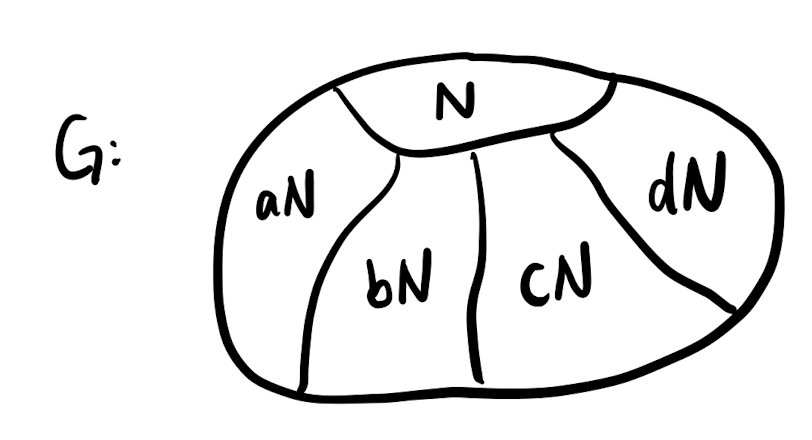
\includegraphics[width = 5cm]{Lecture Files and Images/lec6-3.png}
\end{center}

\subsection{Quotient Groups}

Now that we've defined cosets, we have the following question:
%\textbf{Guiding Question.} 

\begin{qq}
Can we directly define a group structure on the sets of cosets of $N$?
\end{qq}

If $C_1, C_2 \subseteq G$ are cosets, what should $C_1 \cdot C_2$ be? The most intuitive definition would be to take the set of products of each of the elements:

\begin{definition}\label{product of cosets is cosets}
Let the product structure on the cosets be defined as \[C_1 \cdot C_2 \coloneqq \{x \in G: x = y_1 \cdot y_2 ; y_1 \in C_1, y_2 \in C_2\},\]
the pairwise product.
\end{definition}
\begin{theorem}
If $C_1, C_2$ are cosets of a normal subgroup $N$, $C_1 \cdot C_2$ is also a coset of $N.$ 
\end{theorem}

It is \emph{crucial} that $N$ is normal! 
\begin{example}
Consider $H = \{e, y\} \subseteq G = S_3.$ Then $H$ is not a normal subgroup. Consider $xH = \{x, xy\}$. We have \[
xH \cdot xH = \{x^2, x^2y, xyx = y, xyxy = e\},
\]
which is \emph{not} a coset!
\end{example}

\begin{proof}
Let $C_1 = aN$ and $C_2 = bN.$

\begin{itemize}
    \item The inclusion $abN \subseteq C_1 \cdot C_2$ holds because $abn = (ae)(bn) \in C_1 \cdot C_2,$ since $ae \in C_1$ and $bn \in C_2.$ 
    
    \item Take $an_1 \cdot bn_2 \in C_1 \cdot C_2.$ Since $N$ is normal, $bN = Nb,$ so $n_1 \cdot b = b \cdot n_3$ for some $n_3 \in N.$ So 
    \[
    an_1 \cdot bn_2 = abn_3n_2 \in abN.
    \]
\end{itemize}

Then $C_1 \cdot C_2 = abN.$ 

\end{proof}

So it is only when $N$ is normal that we do in fact have a product structure on the set of cosets of $N$!
\begin{definition}\label{quotient group}
The \textbf{quotient group} $G/N$ is the set of cosets of a normal subgroup $N.$ The group structure is defined as\footnote{The notation $[x]$ refers to the equivalence class of $x$ under an equivalence relation; in this case, the equivalence relation is defined by the partition of $G$ into cosets.}
\begin{align*}
[C_1] \cdot [C_2] &\coloneqq [C_1 \cdot C_2] \\
[aN] \cdot [bN] &\coloneqq [abN].
\end{align*}
The right hand side is a coset because $N$ is a normal subgroup.\footnote{The product can be verified to be independent of the representatives $a$ and $b$ from the fact that $N$ is normal.} %\footnote{Did we prove that it is independent of the representatives $a$ and $b$?}
\end{definition}

\begin{theorem}\label{quotient group composition}
The following two statements are true about the quotient group:
\begin{enumerate}
    \item The composition law, as defined in Definition \ref{quotient group} \emph{does} define a group structure on $G/N$ (all the group axioms hold).
    \item There exists a surjective homomorphism 
    \begin{align*}
    \pi: G &\rightarrow G/N \\
    x &\mapsto [xN]
    \end{align*}
    such that $\ker(\pi) = N.$
\end{enumerate}
\end{theorem}

This is one of the most basic operations we can do on groups! 

\begin{proof}

First of all, let's show that $G/N$ is actually a group.
\begin{itemize}
    \item \textbf{Identity.} The identity is $[N] = [eN]$. The product is 
    \[
    [aN] \cdot [N] = [aeN] = [aN].
    \]
    
    \item \textbf{Inverse.} 
    We can check that
    \[
    [aN]^{-1} = [a^{-1}N].
    \]
    
    In general, the inverse of a left coset will be a right coset, but because $N$ is normal, they are the same.  
    
    \item \textbf{Associativity.} Similarly, associativity of $G/N$ boils down to associativity for $G.$\footnote{The proof is left as an exercise for the reader.}
\end{itemize}

Now, we can show the second part of the theorem. Take $\pi(x) = [xN]$. It is evidently a surjective map. Then 
\[
\pi(xy) = [xyN] = [xN] \cdot [yN] = \pi(x) \cdot \pi(y).
\]
Then the kernel is 
\[
\ker(\pi) = \{x \in G : x \in N\} = N.
\]

\end{proof}

Most of the proof of Theorem \ref{quotient group composition} seems very tautological. In fact, most of the action happened earlier on, in Thereom \ref{product of cosets is cosets}, which showed that the product of two cosets actually was another coset, demonstrating that the group structure does makes sense.

Here is an example of how this theorem is often used. 
\begin{example}[Quotient Group of $SL_2(\RR)$]
Take $N = \{\pm I_2\} \nsub G = SL_2(\RR)$. Then, taking the quotient group $SL_2(\RR) / \{\pm I_2\}$ gives a new group $PSL_2(\RR)$.  Thus, from an explicitly defined group, in this case $SL_2(\RR)$, we obtain a new, potentially interesting or useful group by taking a quotient.
\end{example}

Another perspective on $G/N$ is that it is similar to modular arithmetic. We have that $a \equiv b \mod N$ if $aN = bN \subseteq G.$ \footnote{We placed an equivalence relation on the group, and placed a group structure on the equivalence classes.}

\subsection{First Isomorphism Theorem}

Suppose we start off with $G \xrightarrow{f} G'$ a surjective homomorphism, and assume $K = \ker(f)$ is a normal subgroup. Given that it is a normal subgroup, we can feed it into this machine that we have created. Then 
\[
\pi: G \rightarrow G/K
\]
is a surjective group homomorphism. So we have started with a surjective group homomorphism and created another surjective group homomorphism. But in fact, we have done nothing at all! There exists an isomorphism 
\[
\bar{f}: G/K \xrightarrow{\sim} G' .
\]
The diagram 

\begin{center}
% 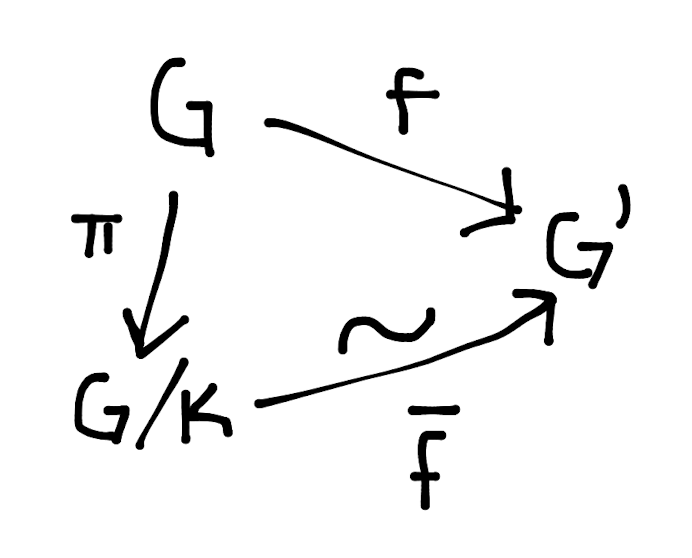
\includegraphics[width = 5cm]{images/lec6-2.png}

% https://tikzcd.yichuanshen.de/#N4Igdg9gJgpgziAXAbVABwnAlgFyxMJZARgBoAGAXVJADcBDAGwFcYkQBxAchAF9T0mXPkIpypYtTpNW7DgHoA0nwEgM2PASLiqNBizaJOfKTCgBzeEVAAzAE4QAtkjIgcEJOJAAjGGCieNIz0vowACkKaoiB2WOYAFjggejKGIAA66RC0MHaMWGAwwDa8KrYOzogATDTugdIG7DZlIPZOSDVuHoiu+rJGmWhYySDBoREaIuyxCUm8lLxAA
\begin{tikzcd}
G \arrow[r, "f"] \arrow[d, "\pi"'] & G' \\
G/K \arrow[ru, "\overline{f}"']    &   
\end{tikzcd}
\end{center}
commutes. 

So $f = \bar{f} \circ \pi.$ So up to isomorphism, our original group homomorphism is the same as our new one. This is not surprising, because there is a correspondence between cosets of the kernel and points in the image. All we are saying is that that bijection is compatible with the group structures on both sides. So $\bar{f}([xk]) = f(x).$ This is known as the \textbf{First Isomorphism Theorem.}

\newpage

\lhead{Lecture 7: Fields and Vector Spaces}
\setcounter{section}{6}
%MIT OpenCourseWare: https://ocw.mit.edu
%RES.18-011 Algebra I Student Notes, Fall 2021
%License: Creative Commons BY-NC-SA 
%For information about citing these materials or our Terms of Use, visit: https://ocw.mit.edu/terms.

\section{Fields and Vector Spaces}
\subsection{Review}
Last time, we learned that we can quotient out a normal subgroup of $N$ to make a new group, $G/N.$

\subsection{Fields}

Now, we will do a hard pivot to learning linear algebra, and then later we will begin to merge it with group theory in different ways. In order to define a vector space, the underlying \emph{field} must be specified.
\begin{definition}
A \textbf{field} $F$ is a set with the operations $(+, \by).$ It must satisfy that 
\begin{itemize}
    \item $(F, +)$ is an abelian group with the usual rules, and
    \item $(F^{\by} \coloneqq F \setminus \{0\}, \by)$ is an abelian group.
\end{itemize}
Also, addition and multiplication must distribute over each other.\footnote{There is some compatibility required.} %add the requirements
\end{definition}

In essence, a field is a set with additive and multiplicative group structures that interact in nice ways.
\begin{example}\label{c r q fields}
The sets $\CC, \RR, $ and $\mathbb{Q}$ are fields, but not $\ZZ,$ since it is not invertible under multiplication.
\end{example}

Since division does not exist in $\ZZ,$ it is not a field. In fact, $\QQ$ is essentially obtained from $\ZZ$ by making it into a field by adding division.

Example \ref{c r q fields} gives us examples of fields with infinitely many elements, but fields can also be constructed that have finite order. Indeed, there is one for every prime number $p.$
\begin{example}[Fields of prime order]
For a prime $p,$ 
\[
(\mathbb{F}_p = \ZZ_p, +, \by)
\]
is a field. If $a \neq 0 \mod p,$ then $\gcd(a, p) = 1$ implies that $ar + ps = 1,$ and so $ar \equiv 1 \mod p,$ and thus $a$ is invertible with multiplicative inverse $r^{-1}.$
\end{example}

However, $\ZZ_6$ is not a field; for example, $2 \mod 6$ has no inverse. In general, $\ZZ_n$ where $n$ is not a prime is not a field, because there will exist some element that is not relatively prime to $n,$ and it will not be invertible. %add the explanation why

\subsection{Vector Spaces}

A vector space, which may be a familiar concept from learning about matrices, can be defined over any field. 
\begin{definition}
A \textbf{vector space} $V$ over a field $F$ is a set $V$ with some operation + such that $(V, +)$ is an abelian group. 
\begin{itemize}
    \item We must be able to scale vectors:
    \begin{align*}
    F &\by V \rightarrow V \\
    (a, \vec{v}) &\mapsto a\vec{v}.
    \end{align*}
    \item Addition and multiplication play nicely and satisfy the usual rules 
    \[
    (\cdots, a(b\vec{v}) = (ab) \cdot \vec{v}, \cdots ).
    \]
    
\end{itemize}
\end{definition}

\begin{example}
For a field $F,$ $F^n$, column vectors with $n$ components $(a_1, \cdots, a_n)^t,$ form a vector space of dimension $n.$
\end{example}

\begin{example}
If $A$ is an $m \by n$ matrix, then 
\[
\{\vec{v} \in F^n : A\vec{v} = (0, \cdots, 0)\}
\]
is a vector space.
\end{example}

\begin{example}
For a homogeneous linear ODE, the solutions form a vector space.
\end{example}

\subsection{Bases and Dimension}

A basis of a vector space is a set of vectors providing a way of describing it without having to list every vector in the vector space.
\begin{definition}
Given $\vec{v}_1, \vec{v}_2, \cdots, \vec{v}_n \in V,$ a \textbf{linear combination} is 
\[
\vec{v} = \sum a_i\vec{v}_i
\]
for $a_i \in F.$
\end{definition}

\begin{definition}
For $S = \{\vec{v}_1, \vec{v}_2, \cdots, \vec{v}_n\}$, the span 
\[
\text{Span}(S) = \{\vec{v} \in V: \vec{v} = \sum a_i \vec{v}_i\}
\]
\end{definition}

This is similar to generating subgroups using elements of a group $G,$ except using the operations of vector spaces.

Artin likes to use the (nonstandard) notation 
\[
\begin{pmatrix}
\vec{v}_1 & \cdots & \vec{v}_n
\end{pmatrix}
\begin{pmatrix}
a_1 \\
\vdots \\
a_n
\end{pmatrix}
\coloneqq \sum a_i \vec{v}_i
\]
for a linear combination. 

\begin{definition}
A set of vectors $S$ \textbf{spans} $V$ if $\text{Span}(S) = V.$ \footnote{There is at least one way of writing $\vec{v}$ as a linear combination.}
\end{definition}

\begin{definition}
A set of vectors $\{\vec{v}_i\}$ is \textbf{linearly independent} if 
\[
\sum a_i \vec{v}_i = \vec{0}
\]
if and only if $a_i = 0$ for all $i.$\footnote{There is at most one way of writing $\vec{v}$ as a linear combination.}

\end{definition}

A basis is both linearly independent and spans.
\begin{definition}
A set of vectors $S = \{\vv{v}_1, \cdots, \vec{v}_n\}$ is a \textbf{basis} if $S$ spans $V$ \emph{and} is linearly independent. Equivalently, each $\vec{v} \in V$ can be written \textbf{uniquely} as $\vec{v} = a_1\vec{v}_1 + \cdots + a_n \vec{v}_n$, where the $a_i$ are called the \textbf{coordinates} of $\vec{v}$ in the basis $S.$
\end{definition}

The standard basis for $\RR^2$ is 
\[
\left\{
\begin{pmatrix}
1 \\
0
\end{pmatrix}, 
\begin{pmatrix}
0 \\
1
\end{pmatrix}\right\}.
\]

In general, when we write a vector $(a, b)^t,$ it represents the linear combination $a(1, 0)^t + b(0, 1)^t.$ 

\begin{example}
Let $V = \RR^2.$ Then the set 
\[
S = \left\{
\begin{pmatrix}
1 \\
1
\end{pmatrix}, \begin{pmatrix}
3 \\
2
\end{pmatrix},
\begin{pmatrix}
2 \\
1
\end{pmatrix}\right\}
\]
spans $\RR^2,$ but is linearly dependent: $\vv{v}_1 - \vv{v}_2 + \vv{v}_3 = \vv{0}.$ But $\{\vv{v}_1, \vv{v}_2\}$ forms a basis. 
\end{example}

A good choice of basis often makes problems easier. 

\begin{definition}
A vector space $V$ is \textbf{finite-dimensional} if $V = \spann(\{\vvv_1, \cdots, \vvv_n\})$ for some $\vv{v}_i \in V.$\footnote{Infinite-dimensional vector spaces are super interesting, but not studied in this class. Real analysis can be used to study them!}

\end{definition}

\begin{lemma}
\label{spanlemma}
If $S = \{\vvv_1, \cdots, \vvv_r\}$ spans $V,$ and $L = \{\vv{w}_1, \cdots, \vv{w}_s\}$ is linearly independent, then 
\begin{enumerate}
    \item Removing elements of $S$ gets a basis of $V.$ 
    \item Adding elements of $S$ to $L$ gets another basis of $V.$
    \item $|S| \geq |L|$.
\end{enumerate}
\end{lemma}

\begin{corollary}
If $S$ and $L$ are both bases for $V,$ then $|S| = |L|.$ Any two bases of $V$ contain the same number of vectors.
\end{corollary}

\begin{proof}
Applying the lemma twice for $S$ and $L$ gives $|S| \geq |L|$ and $|L| \geq |S|.$
\end{proof}

\begin{definition}
The \textbf{dimension} of a vector space $v$ is the size of any basis of $V.$
\end{definition}

\begin{proof}[Proof of Lemma \ref{spanlemma}]

We prove each point separately
\begin{enumerate}
    \item If $S$ is not linearly independent, then there are some $a_i$ such that 
    \[
    \sum_{i=1}^r a_i \vvv_i = \vv{0}.
    \]
    Suppose WLOG that $a_n \neq 0.$ Then \[\vvv_r = a_r^{-1}(-a_1\vvv_1 - \cdots - a_{r-1}\vvv_{r-1}) \in \spann(\vvv_1, \cdots, \vvv_{r-1}).\] If we take $S' = \{\vvv_1, \cdots, \vvv_{r-1}\},$ we have $\spann(S') = \spann(S) = V.$ This is because if we have a linear combination using the vectors of $S$, we can use the equation above to turn it into a combination of vectors in $S'$. We can repeatedly remove until we have a basis of $V.$
    
    \item
    If $S \subset \spann(L)$, then $\spann(L) = V$ so we are done. 
    Otherwise, suppose $\vvv_i \not \in \spann(L)$. We can create $L' = \{\vv{w}_1, \ldots, \vv{w}_s, \vvv_i\}$. 
    Then $L'$ is still linearly independent. 
    We can just keep adding vectors to $L$ so that it stays linearly independent but eventually spans $V.$
    
    \item Each $\vv{w}_j$ is a linear combination of $\vvv_1 , \cdots, \vvv_r.$ Then $\vec{w}_j = \sum_{i = 1}^{r}  a_{ij} \vvv_i$. Let $A$ be the $r \by s $ matrix 
    \[
    A = 
    \begin{pmatrix}
    a_{11} & a_{12} & \cdots & a_{1s}\\
    \vdots & \vdots & \ddots & \vdots \\
    a_{r1} & a_{r2} & \cdots & a_{rs}
    \end{pmatrix}.
    \]
    Then $(\vv{w}_1, \cdots, \vec{w}_s) = (\vvv_1, \cdots, \vvv_r)A.$ Suppose $r < s.$ Then by row-reduction, there exists some nonzero vector $\vv{x}$ such that $A \vv{x} = \vv{0}.$ Then $\sum x_i \vec{w}_i = (\vvv_1, \cdots, \vvv_r)A\vv{x} = \vv{0}.$ This is a contradiction, since $L$ is linearly independent, so $r \geq s.$
\end{enumerate}
\end{proof}

\begin{definition}
A \textbf{linear transformation} is a map 
\[
T: V \rightarrow W
\]
such that 
\[
T(\vv{v}_1 + \vvv_2) = T(\vvv_1) + T(\vvv_2) 
\]
and 
\[
T(a\vvv) = aT(\vvv).
\] We say that $T$ is an \textbf{isomorphism} if it is a bijection $(T^{-1}$ is also an isomorphism). 
\end{definition}
For a vector space $V$ over a field $F$ and a set of vectors $S = \{\vvv_i \in V\},$ we can define the following linear transformation:
\begin{align*}
T_S: F^n &\rightarrow V \\
(a_1, \cdots, a_n) &\mapsto \sum a_i \vvv_i \in V.
\end{align*}

If $S$ is linearly independent, then $T_S$ is injective; if $\spann(S) = V,$ then $T_S$ is surjective, and if $T_S$ is a basis, then $T_S$ is an isomorphism.

\newpage

\lhead{Lecture 8: Linear Transformations with Bases and the Dimension Formula}
\setcounter{section}{7}
%MIT OpenCourseWare: https://ocw.mit.edu
%RES.18-011 Algebra I Student Notes, Fall 2021
%License: Creative Commons BY-NC-SA 
%For information about citing these materials or our Terms of Use, visit: https://ocw.mit.edu/terms.

\section{Dimension Formula}
\subsection{Review}
Last time, we ended off with the definition of linear transformations.
\subsection{Matrix of Linear Transformations}
Given a linear transformation $T: V \rightarrow W$, we know 
\[ T(a_1 \vvv_1 + \cdots + a_n \vvv_n) = a_1 T(\vvv_1) + \cdots + a_n T(\vvv_n) .\]
Then, given any basis $\vvv_1, \ldots , \vvv_n$ for $V$, the above property tell us that $T$ is completely determined by the values of $T(\vvv_1), \ldots, T(\vvv_n)$. 

\begin{example} \label{basistrans}
    Last time, we discussed a linear transformation from column vectors to another vector space. 
    In particular, if we have a basis $\vv{w}_1, \ldots, \vv{w}_m $ of $W$, then we can create the following linear transformation:
    \begin{align*}
        B: F^n &\rightarrow W \\
        \vv{e}_i & \mapsto \vv{w}_i \\
        (a_1, \cdots, a_n) &\mapsto \sum a_i \vv{w}_i,
    \end{align*}
    where $\vv{e}_i$ is the zero column vector with a 1 in the $i$th position.
    This is an isomorphism due to choosing $\vv{w}_i$ to be a basis. 
    The inverse map $B^{-1}(\vv{w}) = (a_1, \cdots, a_n)$ sends a vector to the \emph{coordinates} of $\vv{w}$ for the given basis.
    % maybe this should go in review? i think it wasn't exactly covered last time though
\end{example}
\begin{example}
    There is a bijection between matrices $A \in \text{Mat}_{m\times n} (F)$ and linear transformations $T : F^n \rightarrow F^m$.
    For every matrix $A$, it can be mapped to the linear transformation $T = A\cdot \vv{x}$.
    For every transformation $T$, it can be mapped to 
    \[A = \begin{pmatrix} T(\vv{e}_1) & T(\vv{e}_2) &\cdots  & T(\vv{e}_n) \end{pmatrix}. \]

    Both the set of matrices and the set of linear transformations are vector spaces, so this defines an isomorphism between two vector spaces. We will switch between these notions frequently.

    As a special case, if we have an isomorphism $T : F^n \xrightarrow{\sim} F^m$, then this forces $m = n$ and the corresponding matrix $A$ must be in $\GL_n(F)$.
\end{example}
From Example \ref{basistrans}, suppose we have two different bases of $V$ and create their corresponding linear transformations $B$ and $B'$. Let the corresponding bases be $\{\vvv_1, \ldots, \vvv_n \}$ and $\{ \vv{w}_1, \ldots, \vv{w}_n \}$ respectively.
Then, $P \coloneqq B^{-1} \circ B'$ defines a mapping from $F^n$ to $F^n$, and we must have $P \in GL_n(F)$.
Furthermore, $B' = B \circ P$. These relations can be seen by following the arrows in the below diagram:
\[
\begin{tikzcd}
F^n \arrow[r, "B"] & V \\
& F^n \arrow[lu, "P"] \arrow[u, "B'"]
\end{tikzcd}
\]
We can figure out the columns of $P$ as well: 
\[P(\vv{e}_i) = B^{-1} (B'(\vv{e}_i)) = B^{-1}(\vv{w}_i).\]
We know $B^{-1}(\vv{w}_i)$ is just the coordinates of $\vv{w}_i$ for the basis $\{\vvv_1, \ldots, \vvv_n \}$. 
Similarly, we can figure out the columns of $P^{-1}$ by taking the each $\vvv_i$ and writing it in terms of the basis of $\vv{w}$'s.

Given a vector $\vvv \in V$, we can write the coordinates $\vv{x} = B^{-1}(\vvv)$ and $\vv{x}' = (B')^{-1} (\vvv)$. The coordinates are related by $P\vv{x}' = \vv{x}$ and $P^{-1}\vv{x} = \vv{x}'$ by using our expression for $P$.

For any finite-dimensional vector space, by picking a basis, we can write every vector in terms of coordinates. 
Then, for every transformation $T: V \rightarrow W$, we can write it as a matrix $A$ using coordinates. 
Suppose we have the coordinate maps $B: F^n \rightarrow V$ and $C : F^m \rightarrow W$ and the respective bases are $\{ \vvv_i\}$ and $\{ \vv{w}_i \}$.
\[
\begin{tikzcd}
V \arrow[r, "T"] & W \\
F^n \arrow[u, "B"]\arrow[r, "A"] & F^m \arrow[u, "C"]
\end{tikzcd}
\]
Following the arrows, we have $A \coloneqq C^{-1} \circ T \circ B \in \text{Mat}_{m\times n}(F)$.
To write down $A$, we can find the $i$th column of $A$ by writing $T(\vvv_i)$ in terms of the $\vv{w}$'s.

\begin{example} 
    Let's see an example of computing $A$.
    Let $V$ be the set of complex functions such that $f''(t) = f(t)$.
    Let $W$ be the set of complex functions such that $f''(t) = -f(t)$. 
    We can define the transformation 
    \begin{align*}
        T:V &\rightarrow W \\
        f(t) &\mapsto f(it) .
    \end{align*}
    Note that $T$ looks nothing like a matrix right now, but we can turn it into one by picking bases for $V$ and $W$. One choice of basis is $V = \spann(e^t, e^{-t})$ and $W = \spann(\cos t, \sin t)$. 

    Then, by writing $T(e^t) = e^{it} = \cos t + i \sin t$ and $T(e^{-t}) = e^{-it} = \cos t + -i \sin t$, we have found the columns of $A$:
    \[A = \begin{pmatrix} 1 & 1 \\ i & -i \end{pmatrix} .\]

    If we had chosen a different basis for $W = \spann(e^{it}, e^{-it})$, then our matrix $A'$ would just be the identity matrix.

\end{example}


\begin{qq}
    We have seen that the same linear transformation leads to different $A$, so can we pick bases so that $A$ ``looks very nice"? For example, in the previous example, we were able to make $A$ the identity matrix by picking a different basis. 
\end{qq}
We will answer this question at the end of the next section.
\subsection{Dimension Formula}
Note that linear transformations are very similar to group homomorphisms. 
They are both mappings that preserve the structure that we care about. 
We can define and prove similar results as the ones we showed for group homomorphisms.

\begin{definition}
    Given a linear transformation $T : V \rightarrow W$, we can define the \textbf{kernel} and \textbf{image}.
    \begin{align*}
        \Ker(T) &\coloneqq \{ \vvv \mid T(\vvv) =\vv{0} \} \\
        \im(T) &\coloneqq \{ \vv{w} \mid T(\vvv) \vv{w} \text{ for some $\vvv \in V$} \} 
    \end{align*}
    By similar logic to group homomorphisms, these are vector \emph{subspaces} of $V$ and $W$ respectively.
    We also define the \textbf{nullity} and the \textbf{rank} as the dimension of the kernel and image respectively.
\end{definition}

\begin{theorem}[Dimension formula]
    Given $T : V \rightarrow W$,
    \[\dim(\Ker T ) + \dim (\im T) = \dim (V). \]
\end{theorem}
This is somewhat reminiscent of the theorem on groups $|G| = \lvert\Ker(G)\rvert \lvert\im(G)\rvert$.
\begin{proof}
    Pick $\vvv_1, \ldots, \vvv_k$ as a basis for $\Ker(T)$. 
    From a theorem from last class, we can add vectors $\vvv_{k+1}, \ldots, \vvv_n$ to get a basis for $V$ where $n = \dim V$ and $k = \dim( \Ker(T))$.

    Let $\vv{w}_i \coloneqq T(\vvv_i)$. By the definition of kernel, $\vv{w}_i = 0$ for $1 \leq i \leq k$. 
    We will show that $\{\vv{w}_{k+1}, \ldots, \vv{w}_n \}$ is a basis for $\im(T)$, so that \[\text{rank}(T) = n-k = \dim(V) - \dim(\Ker(T)). \] 
    To prove that it is a basis, we need to show that they are linearly independent and they span $\im(T)$.
    For the span,
    \begin{align*}
        \im(T) &= \spann(T(\vvv_1), \ldots, T(\vvv_n))\\
               &= \spann(T(\vvv_{k+1}), \ldots, T(\vvv_n)) \\
               &= \spann(\vv{w}_{k+1}, \ldots, \vv{w}_n).
    \end{align*}
    For linear independence, we consider the solutions to: 
    \[ a_{k+1} \vv{w}_{k+1} + \cdots + a_n \vv{w}_n = \vv{0}. \]
    This implies that 
    \[ T(a_{k+1} \vv{v}_{k+1} + \cdots + a_n \vv{v}_n) = \vv{0} \]
    and thus 
    \[ a_{k+1} \vv{v}_{k+1} + \cdots + a_n \vv{v}_n \in \Ker(T) .\]
    Since $\vvv_1, \ldots, \vvv_k$ is a basis for the kernel, there must exist coefficients $a_1, \ldots, a_k$ such that 
    \[ a_{k+1} \vv{v}_{k+1} + \cdots + a_n \vv{v}_n = a_1 \vvv_1 + \cdots + a_k \vvv_k. \]
    However, this forces $a_i = 0$ for all $i$ since the $\vvv$'s form a basis for $V$. 
    Therefore, $\{\vv{w}_{k+1}, \ldots, \vv{w}_n \}$ are linearly independent and thus a basis of $\im(T)$.
\end{proof}
The proof of the dimension formula shows a bit more. 
Using the same notation as in the proof, take a basis for $V$ to be $\vvv_{k+1}, \ldots, \vvv_n, \vvv_1, \ldots, \vvv_k$. This is essentially the same basis, but permuted so that the coordinate vectors are also permuted. 
We extend the basis for $\im(T)$ to a basis for $W$ with the vectors $\vv{w}_{k+1} , \ldots, \vv{w}_n, \vv{u}_1, \ldots, \vv{u}_r$. 
Then we find the matrix for $T$ by writing down the coordinates of $T(\vvv_i)$ with respect to the $\vv{w}$'s. 
When $k+1 \leq i \leq n$, $T(\vvv_i) = \vv{w}_i$. When $1 \leq i \leq k$, $T(\vvv_i) = 0$.
Our matrix for $T$ is particularly simple (written in block form):
\[A=
\begin{pmatrix}
    I_{n-k} & 0 \\
    0 & 0
\end{pmatrix}.\]
\begin{corollary}
    For any linear transformation, we can write its matrix in the above form for some choice of basis for $V$ and $W$.
\end{corollary}
\begin{corollary}
As a special case, if we already are given a matrix $M \in \text{Mat}_{m\times n}$ representing a linear transformation from $F^n \rightarrow F^m$, then there exists change of basis matrices $P \in \GL_n(F), Q \in \GL_m(F)$ such that $Q^{-1} M P$ is in the above form.
Pictorially, this looks like: 
\[
\begin{tikzcd}
F^n \arrow[r, "M"] & F^m \\
F^n \arrow[u, "P"]\arrow[r, "A"] & F^m \arrow[u, "Q"]
\end{tikzcd}
\]
\end{corollary}


\newpage

\lhead{Lecture 9: Eigenvectors, Eigenvalues, and Diagonalizable Matrices}
\setcounter{section}{8}
%MIT OpenCourseWare: https://ocw.mit.edu
%RES.18-011 Algebra I Student Notes, Fall 2021
%License: Creative Commons BY-NC-SA 
%For information about citing these materials or our Terms of Use, visit: https://ocw.mit.edu/terms.

\section{Dimension Formula}
\subsection{Review}

Last time, we discussed linear transformations between two vector spaces. By picking a basis cleverly, it is possible to write the matrix of the linear transformation in a very nice form. For example, given a linear transformation $M: F^n \rto F^m,$ by changing the bases for $F^n$ and $F^m$ with the invertible matrices $P$ and $Q,$ the matrix $A$ will have a very simple form. 
\[
\begin{tikzcd}
F^n \arrow[r, "M"] & F^m \\
F^n \arrow[u, "P"]\arrow[r, "A"] & F^m \arrow[u, "Q"]
\end{tikzcd}
\]

With appropriate bases, 
\[
A = Q^{-1} M P = \begin{pmatrix} I_k & 0 \\ 0 & 0 \end{pmatrix},
\]

where $A$ is an $m \by n$ matrix with the identity in the top left corner. The first $k$ columns correspond to the image and the last $n - k$ columns correspond to the kernel. As a corollary, it is possible to see the \textbf{dimension formula} \[\dim \im (A) + \dim \ker(A) = n.\]

\begin{corollary}
Given a matrix $M \in \text{Mat}_{m \by n} (F),$ we have \[\text{rank}(M) = \text{rank}(M^T).\]
\end{corollary}

Essentially, this corollary states that the dimension of the span of the columns is the same as the dimension of the span of the rows, which is surprising! The first is a subspace of $F^m,$ while the second is a subspace of $F^n,$ but they still have the same dimension.
\begin{proof}[Sketch of Proof.]
This theorem is clearly true for $A,$ since the row-rank and the column-rank are both just $k$. However, since $A$ and $M$ differ by isomorphisms $P$ and $Q$, the rank of $A$ is the same as the rank of $M.$ Similarly, the rank of $A^T$ is also equal to the rank of $M^T.$ Therefore, \[\text{rank}(M) = \text{rank}(M^T).\]
\end{proof}

We are not going to use this often in this course, but this is a fact emphasized in traditional linear algebra classes. 

\subsection{Linear Operators}

Today, we will specialize the discussion on arbitrary linear transformations to \textbf{linear operators}, which go from a vector space to itself.

\begin{definition}
A \textbf{linear operator} is a linear transformation \[T: V \rto V.\] 
\end{definition}

Let's see some examples.
\begin{example}\label{rotation by theta}
Let $V = \RR^2.$ Then, $T$ is the linear transformation that is rotation by angle $\theta$ counterclockwise. This goes from the vector space to itself.
\end{example}

\begin{example}\label{derivative}
Let $V = \{\text{polynomials of degree} \leq 2\}.$ Then the derivative $T(f(t)) = f'(t)$ is a linear operator.
\end{example}

The first natural question to ask about linear operators is working out the matrix of the linear transformation upon picking a basis. The only difference between this discussion and the discussion on linear transformations is that here, the transformation is from a vector space to itself, so once a basis has been picked, both sides have a fixed basis. For general linear transformations from a vector space to a different vector space, two different bases can be picked. 

\begin{qq}
What is the matrix of a linear operator on a vector space with a chosen basis?
\end{qq}

Consider a basis \[B: F^n \rto V.\] Then $T$ becomes a square matrix $A \in \matnn(F).$ 

For Example \ref{rotation by theta}, picking the basis standard basis gives a rotation matrix: \[\left\{\begin{pmatrix}1 \\ 0\end{pmatrix}, \begin{pmatrix}0 \\ 1\end{pmatrix}\right\} \rightsquigarrow A = \begin{pmatrix} \cos\theta & -\sin\theta \\ \sin\theta & \cos\theta\end{pmatrix}.\] This is determined by figuring out where the $i$th basis vector is mapped, which is the $i$th column.

For Example \ref{derivative}, it is also possible to write down a matrix: \[\{1, t, t^2\} \rightsquigarrow A = \begin{pmatrix}
0 & 1 & 0 \\
0 & 0 & 2 \\
0 & 0 & 0
\end{pmatrix}.\]

This should all be reminiscent of the previous section. 

\begin{proposition}
When working with linear operators $T: V \rto V$, for $V$ finite-dimensional\footnote{In this class, the implicit assumption will always be that we are working with finite-dimensional vector spaces}, then \[T \text{ is injective }\leftrightarrow T \text{ is surjective }\leftrightarrow \text{ is an isomorphism.}\]
\end{proposition}

In fact, this fact is true for maps from a finite set to itself. Finite-dimensional vector spaces can be infinite, but have the same property.

\begin{proof}
Using the dimension formula, 
\[\dim \ker T + \dim \im T = \dim V.\] If $T$ is injective, then $\dim\ker T = 0,$ which is true if and only if $\dim\im T = \dim V,$ which means that $T$ is surjective. 
\end{proof}

So finite-dimensional vector spaces behave a lot like finite sets. 

\subsection{Change of Basis}

Now, the next natural question to ask is about changing bases. 
\begin{qq}
What happens to a matrix for $T: V \rto V$ upon changing basis for $V$?
\end{qq}

Specifying a basis for $V$ determines a diagram  \[
\begin{tikzcd}
V \arrow[r, "T"] & V \\
F^n \arrow[u, "B"]\arrow[r, "A"] & F^m \arrow[u, "B"]
\end{tikzcd}.
\]

A new basis comes from an invertible matrix $P \in GL_n(F)$, where the new basis is $B' = B \cdot P,$ and determines an extended diagram 
\[\begin{tikzcd}
V \arrow[r, "T"] & V \\
F^n \arrow[u, "B"]\arrow[r, "A"] & F^n \arrow[u, "B"] \\
F^n \arrow[u, "P"] \arrow[uu, bend left=49, "B'"] \arrow[r, "A'"] & F^n \arrow[u, "P"] \arrow[uu, bend right=49, "B'"]
\end{tikzcd}.
\]

There is a new matrix $A'$ that represents the same linear transformation $T.$ The difference between this case and the general case is that the bases are the same on either side of the transformation, and there is no longer the freedom to choose different bases for the domain and the codomain. 

The new matrix, by following the arrows on the diagram, is \[A' = P^{-1}AP.\] The matrix $A'$ is related to $A$ by conjugation by $P.$ 

\begin{definition}
A matrix $A'$ is \textbf{similar} to $A$ if there exists some $P \in GL_n(F)$ such that \[A' = P^{-1}AP.\]
\end{definition}
Similar matrices arise from the same linear operator from a vector space to itself, but with different bases picked. Again, to emphasize, the difference between today's case, $T: V \rto V$, and the case in the last section, $T: V \rto W$, is that in the first case there is only one base change matrix $P,$ instead of $P$ and $Q,$ since the matrix must operate the same on the left and right sides.


As an result, given a vector space $V$ and an operator $T: V \rto V,$ it is possible to define the determinant of $T$ \emph{without} having to specify a basis. The vector space $V$ might be a vector space without a canonical basis, but it is still possible to define the determinant. Picking any basis of $V$ produces a square matrix $A$, and the determinant would then be $\det(T) = \det(A).$ In fact, from the base change formula, it is clear that the determinant does not depend on which basis is used! From a different basis, \[\det(A') = \det(P^{-1}AP) = \det(P)^{-1}\det(A)\det(P) = \det(A),\] since the determinant is multiplicative. As a result, it is possible to define the determinant of $T$ independently of the choice of basis\footnote{It doesn't depend on which basis was chosen, so any basis works}, and so $\det(T)$ has a meaning outside of a particular basis. For example, on $\RR^n,$ the determinant represents a "volume," which is independent of the particular choice of basis. Here, we are saying that even for fields like finite fields, where "volume" may not make sense, the determinant still has some intrinsic meaning.

\subsection{Eigenvectors, Eigenvalues, and Diagonalizable Matrices}
Our discussion leads to the following question, which is the same as last class, but for linear operators.
\begin{qq}
How nice can we make $A$ by changing basis of $V$?
\end{qq}

Last class, it was possible to make the matrix extremely nice, since we could pick a basis for the domain \emph{and} for the codomain. Now, let's see an example for when the domain is the same vector space as the codomain. 

\begin{example}\label{diagonal matrix}
Let $V = \RR^2.$ Consider \[A = \begin{pmatrix} 2 & 3 \\ 3 & 2 \end{pmatrix}.\] We see that \[A \begin{pmatrix} 1 \\ 1 \end{pmatrix} = \begin{pmatrix} 5 \\ 5 \end{pmatrix} =  5\begin{pmatrix} 1 \\ 1 \end{pmatrix}\] and \[A\begin{pmatrix} -1 \\ 1 \end{pmatrix} = \begin{pmatrix} 1 \\ -1 \end{pmatrix} = -1 \begin{pmatrix} -1 \\ 1 \end{pmatrix}.\]

The operator is scaling the vector $(1, 1)$ and flipping the vector $(-1, 1),$ and the transformation on any other vector will be a combination of these two moves, scaling and flipping. In particular, taking \[P = \begin{pmatrix} 1 & -1 \\ 1 & 1\end{pmatrix},\] which has the first vector as the first column and the second vector as the second column, gives \[A' = P^{-1}AP = \begin{pmatrix} 5 & 0 \\ 0 & -1 \end{pmatrix}.\]

\begin{center}
    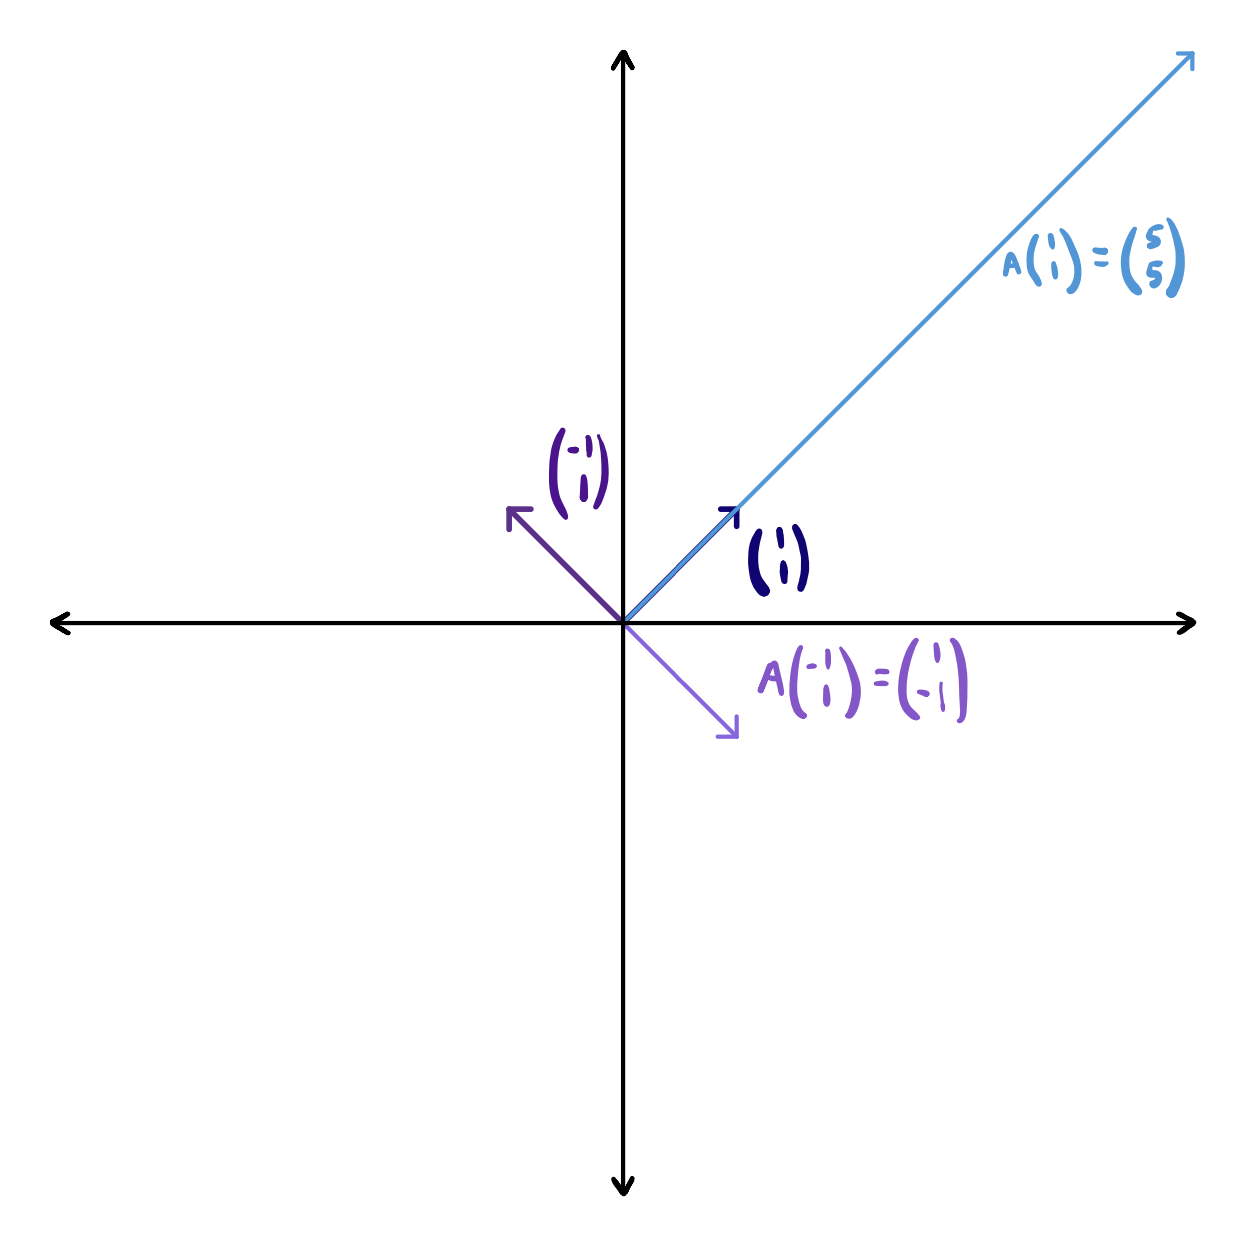
\includegraphics[width=8cm]{Lecture Files and Images/lec9-1.png}
\end{center}

\end{example}

In the new basis, it is possible to make the matrix diagonal! Making the matrix diagonal makes it possible to see how it operates, which is stretching by 5 in one direction, and flipping in the other direction (both independently of the other direction). 

In general, we will really want to be able to make matrices diagonal, since it allows us to see what it is doing in the direction of each basis vector, independently of the other directions (as there are 0s in the matrix elsewhere). This gold standard type of vector will be called an \textbf{eigenvector}.

\begin{definition}
A vector $v \neq 0$ is an \textbf{eigenvector} if \[Tv = \lambda v\] for some $\lambda \in F,$ and $\lambda$ is called an \textbf{eigenvalue}.
\end{definition}

When an operator is applied to a vector, the result is proportional to the vector. The operator maintains the direction of the vector, and just scales it. Obviously, scaling an eigenvector by some nonzero scalar also results in another eigenvector.

\begin{example}
For Example \ref{diagonal matrix}, the vector $\begin{pmatrix} 1 \\ 1 \end{pmatrix}$ is an eigenvector with eigenvalue 5, and $\begin{pmatrix} -1 \\ 1 \end{pmatrix}$ is an eigenvector with eigenvalue -$1.$
\end{example}

This example is special because not only are there eigenvectors, there are enough to form a basis. 

\begin{definition}
A basis $\{v_1, \cdots, v_n\}$ of $V$ where each $v_i$ is an eigenvector; that is, \[Tv_i = \lambda_i v_i,\] then the basis is called an \textbf{eigenbasis}.
\end{definition}

In an eigenbasis, the matrix for $T$ is \[\begin{pmatrix} \lambda_1 & \cdots & 0 \\
\vdots & \ddots & \vdots \\
0 & \cdots & \lambda_n\end{pmatrix},\] which is diagonal with $\lambda_i$ in the $(i, i)$th entry. 

Diagonal matrices are extremely nice. In general, it is very hard to take matrices to high powers, but for diagonal matrices, each entry is simply raised to that power.

\begin{definition}
If a linear operator has an eigenbasis $T,$ it is called \textbf{diagonalizable}.
\end{definition}

An equivalent definition holds for matrices.

\begin{definition}
Given a matrix $A,$ if there exists some invertible $P$ such that \[P^{-1}AP = D\] for some diagonal matrix $D$, then $A$ is called \textbf{diagonalizable}.
\end{definition}

That is, $A$ is diagonalizable if it is similar to a diagonal matrix. 

The key concept is that an eigenbasis provides the directions in which the operator $T$ behaves nicely by simply scaling or flipping a vector in that direction.
\subsection{Finding Eigenvalues and Eigenvectors}
 Unfortunately, not every matrix is diagonalizable, but the focus for the next few classes will be finding eigenvectors, eigenvalues, and eigenbases, assuming that a matrix \emph{is} diagonalizable.

\begin{qq}
How do we find eigenvectors, eigenvalues, and eigenbases?
\end{qq}

\begin{itemize}
    \item \textbf{Step 1.} Perhaps unintuitively, the first step is to find possible eigenvalues! Given a matrix $A \in \matnn(F)$ in some less good basis, we want to find eigenvectors that form a better basis that is an eigenbasis, so that $A$ will be diagonal and have a nicer form. 
    
    Suppose $\lambda$ is an eigenvalue for $A.$ Then there exists some nonzero $v$ such that \[Av = \lambda v,\] by definition. (There may be lots of $v,$ and in fact scaling any $v$ will produce another eigenvector, but for a given $\lambda$ we just want to know if there is a $v$ at all.) We know that \[\lambda v = \lambda I_n v,\] so this is equivalent to \[(\lambda I_n - A) v = 0\] for some $v.$ That is, the kernel is nontrivial: \[\ker(\lambda I_n -A) \neq \{\vec{0}\}.\] This is equivalent to \[\lambda I_n - A \text{ is not invertible,}\] which happens if and only if \[\det(\lambda I_n - A) = 0.\] This is not bad at all! The determinant is a formula that we can just calculate. 
    
    So in fact, we want to look for $\lambda$ such that the equation\[\boxed{\det(\lambda I_n - A) = 0}.\]  holds. It is customary in this context to replace $t$ with $\lambda,$ and so with $t$ as the variable, we have \[p(t) \coloneqq \det(t I_n - A),\] which is a polynomial of degree $n$ in $t$ called the \textbf{characteristic polynomial}.
    
    \begin{example}
    Given \[A = \begin{pmatrix} 2 & 3 \\ 3 & 2\end{pmatrix},\] we have the characteristic polynomial \[p_A(t) = \det\begin{pmatrix} t - 2 & -3 \\ -3 & t - 2\end{pmatrix} = (t-2)(t-2) - (-3)(-3) = t^2 - 4t - 5.\]
    \end{example}
    
    In general, where $A = (a_{ij}),$ we have \[p_A(t) = \det\begin{pmatrix} t - a_{11} & \cdots & \star \\
    \vdots & \ddots & \vdots \\
    \star & \cdots & t - a_{nn}
    \end{pmatrix} = t^n + \cdots ,\] which is a degree $n$ polynomial in $t.$
    
    If $A'$ is similar to $A,$ then they have the same characteristic polynomial, since the determinant is basis-invariant. 
    
    \begin{proposition}
    Given $\lambda \in F,$ $\lambda$ is an eigenvalue for $A$ if and only if $p_A(\lambda) = 0$; that is, if and only if $\lambda$ is a root of $p_A(t).$
    \end{proposition}
    
    For example, for our earlier example, the eigenvalues would be $-1$ and $5$, since $t^2 - 4t - 5 = (t + 1)(t - 5).$
    
    As a caveat, if $F$ is an arbitrary field, there may not be any roots. For example, a rotation matrix over $\RR$ does not have any real eigenvalues. However, if $F = \CC,$ there will always be $n$ roots (not necessarily distinct), and so there will always be eigenvalues. 
    
    \item \textbf{Step 2.} For each eigenvalue, find the associated eigenvectors. For each $\lambda,$ we want to take a vector in $\ker(\lambda I_n - A),$ which by assumption is a nonzero subspace. Using Gaussian elimination or row operations, we can mechanically compute a basis for $\ker(\lambda I_n - A),$ although we will not spend a lot of time on this. 
    
    \begin{example}
    For $\lambda = 5,$ we have \[5 \cdot I_2 - A = \begin{pmatrix} 3 & -3 \\ -3 & 3 \end{pmatrix},\] and the kernel is \[\ker = \spann \left\{\begin{pmatrix} 1 \\ 1 \end{pmatrix}\right\}.\]
    \end{example}
    
    We will say more about this next lecture!
\end{itemize}

\newpage

\lhead{Lecture 10: The Jordan Decomposition}
\setcounter{section}{9}
%MIT OpenCourseWare: https://ocw.mit.edu
%RES.18-011 Algebra I Student Notes, Fall 2021
%License: Creative Commons BY-NC-SA 
%For information about citing these materials or our Terms of Use, visit: https://ocw.mit.edu/terms.

\section{Eigenbases and the Jordan Form}


Change of basis is a powerful tool, and often, we would like to work in as natural a basis as possible.

\begin{qq}
Given a linear operator, how can we find a basis in which the matrix is as nice as possible?
\end{qq}
\subsection{Review}
Last time, we learned about eigenvectors and eigenvalues of linear operators, or more concretely, matrices, on vector spaces. An \textbf{eigenvector} is a (nonzero) vector sent to itself, up to scaling, under the linear operator, and its associated \textbf{eigenvalue} is the scaling factor; that is, if $A\vec{v} = \lambda\vec{v}$ for some scalar $\lambda,$ $\vec{v}$ is an eigenvector with associated eigenvalue $\lambda.$

If there exists an eigenbasis\footnote{A basis consisting of eigenvectors}, then in that basis, the linear operator $P^{-1}AP$\footnote{This comes from the change of basis formula} will simply become $\begin{pmatrix}
\lambda_1 & \cdots & 0 \\
0 & \ddots & 0 \\
0 & \cdots & \lambda_n
\end{pmatrix},$ since each basis vector $\vec{v}_i$ is sent to $\lambda_i\vec{v}_i.$ So having an eigenbasis is equivalent to the matrix $A$ being similar to a diagonal matrix.

In order to concretely find the eigenvectors, it is easier to first find the eigenvalues, which are the roots of the \textbf{characteristic polynomial} $p_A(t) =\det\left(tI_n - A\right)$. Each root $\lambda$ of $p_A$ has at least one corresponding eigenvector. The eigenvectors for $\lambda$ are precisely the nonzero vectors in $\ker(\lambda I_n - A).$


\subsection{The Characteristic Polynomial}
Let's start with an example. 
\begin{example}
If $A = \begin{pmatrix}
a & b \\ c & d
\end{pmatrix}$, then $p_A(t) = t^2 - (a + d)t + (ad -bc).$
\end{example}
 In general, for an $n \by n$ matrix,
\[
p_A(t) = t^n - (a_{11} + \cdots + a_{nn}) t^{n-1} + (-1)^n \det(A).
\] The coefficient of $t^{n-1}$ is the sum of the entries on the diagonal, called the \textbf{trace} of $A.$ 

% \begin{qq}
% What can we learn from the characteristic polynomial? 

% \end{qq}

Because the characteristic polynomial can be written as a determinant, it can be defined for general linear operators without specifying a basis, and so each of the coefficients are basis-independent. In particular, we get that 
\[
\trace(P^{-1}AP) = \trace(A).
\]

\begin{qq}
What can go wrong when hunting for an eigenbasis? How can we fix this?
\end{qq}

\begin{example}
Over the real numbers $\RR,$ take $A = \begin{pmatrix}
\cos\theta & -\sin\theta \\
\sin\theta & \cos\theta
\end{pmatrix}$. The characteristic polynomial is $p_A(t) = t^2 - 2\cos\theta + 1,$ which has no real roots (unless $\theta = \pi$.) Geometrically, that makes sense, because under a rotation by $\theta \neq k\pi$, every vector will end up pointing an a different direction than it initially was, so there should be no real eigenvectors.
\end{example}

Over a general field $F,$ it is certainly possible for the characteristic polynomial not to have any roots at all; in order to fix this issue, we work over a field like $\CC,$\footnote{Fields where every non-constant polynomial has roots are called \textbf{algebraically closed}.} where every degree $n$ polynomial always has $n$ roots (with multiplicity). So $p_A(t) = (t - \lambda_1) \cdots (t - \lambda_n),$ where the $\lambda_i$ can repeat. For the rest of the lecture, we will only consider linear operators on vector spaces over $\CC,$ which takes care of the first obstacle of finding eigenvalues.

However, even over $\CC,$ not every linear operator has an eigenbasis. 
\begin{example}
Consider $A = \begin{pmatrix}
0 & 1 \\ 0 & 0
\end{pmatrix}$. The characteristic polynomial is $p_A(t) = t^2,$ so if $A$ were similar to some diagonal matrix, it would be similar to the zero matrix; this would mean that $A$ would be the zero matrix, and thus $A$ cannot be diagonalizable. 

In other words, $p_A(t)$ only has one root, 0, so any eigenvector would be in $\ker(0 I_2 - A) = \spann(\vec{e}_1).$ So there is only a one-dimensional space of eigenvectors, which is not enough to create an eigenbasis. 
\end{example}

In some sense, which we will make precise later on in this lecture, this is the most important counterexample for why linear operators can be nondiagonalizable.

\begin{proposition}\label{linindp eigenvectors}
Given an $n \by n$ matrix $A$, eigenvectors $\vec{v}_1, \cdots, \vec{v}_k,$ and distinct eigenvalues $\lambda_1, \cdots, \lambda_k,$ the vectors $\vec{v}_i$ are all linearly independent.
\end{proposition}
\begin{proof}
Let's prove this by induction. 



\textbf{Base Case.} If $k = 1,$ by the definition of an eigenvector, $\vec{v}_k \neq 0$ so $\{\vec{v}_i\}$ is linearly independent. 

\textbf{Inductive Hypothesis.} Suppose the proposition is true for $k - 1.$ 

\textbf{Inductive Step.} Now, suppose the proposition is not true for $k$. Then there exist coefficients $a_i$ such that \[\sum a_i \vec{v}_i = 0.\] Applying $A$ to both sides, we get 
\[
\sum a_i\lambda_i \vec{v}_i = 0,
\]
which is another linear relation between the $k$ vectors. Subtracting $k$ times the first relation from the second one results in the linear relation 
\[
\sum a_i(\lambda_i - \lambda_k) = \sum_{i = 0}^{i = k-1} a_i(\lambda_i - \lambda_k) = 0.
\]
Since in the last term $\lambda_k - \lambda_k = 0,$ while $\lambda_i - \lambda_k \neq 0$ for $i \neq k$ since the $\lambda_i$ are distinct, we obtain a linear relation between $\vec{v}_1, \cdots, \vec{v}_{k - 1},$ which is a contradiction of the inductive hypothesis. Thus, $\{v_i\}_{i = 0, \cdots, k}$ is linearly independent. 
\end{proof}

\begin{corollary}
Consider a matrix $A$. If the characteristic polynomial is 
\[
p_A(t) = (t - \lambda_1) \cdots (t - \lambda_n)
\]
where each $\lambda_i$ is distinct, $A$ will have an eigenbasis and will thus be diagonalizable. 
\end{corollary}
\begin{proof}
Each eigenvalue must have at least one eigenvector. Taking $\vec{v}_1, \cdots, \vec{v}_n$ to be eigenvectors for $\lambda_1, \cdots, \lambda_n$. Since there are $n$ eigenvectors, which is the same as the dimension of the vector space, and by Proposition \ref{linindp eigenvectors} they are linearly independent, they form an eigenbasis and $A$ is diagonalizable. 
\end{proof}

If there are repeated roots, then there will not necessarily be enough eigenvectors to form a basis. Luckily for us, it is usually true that a matrix will be diagonalizable.\footnote{More concretely, the space of $n \by n$ square matrices can be thought of as a metric space, and the non-diagonalizable matrices will be a set of measure zero. In particular, the diagonalizable matrices are \textbf{dense} in the space of all square matrices. Intuitively, given a non-diagonalizable matrix, perturbing the entries by a little bit will perturb the roots a little bit, making them non-distinct.}

In general, $p_A(t) = (t-\lambda_1)^{e_1}\cdots(t-\lambda_k)^{e_k}$, where the $\lambda_i$ are distinct. Let $V_{\lambda_i} = \ker(\lambda_i I - A).$ Any vector $v \in V_{\lambda_i}$ is an eigenvector with eigenvalue $\lambda_i.$ We know that for each $i,$ $\dim V_{\lambda_i} \geq 1$. Using our proposition, given a basis for each subspace $V_{\lambda_i},$ if there are enough to get $n$ total vectors, combining all the bases would give an eigenbasis for $A$, since they would all be linearly independent.\footnote{Computationally, it is simple to find basis vectors, and in a more computational class we would go further in-depth on finding these.} 

\subsection{Jordan Form}

Keeping in mind the matrix $A = \begin{pmatrix}
0 & 1 \\ 0 & 0
\end{pmatrix}$, we have the following question.
\begin{qq}
If a matrix is \emph{not} diagonalizable, what is nicest form it can take on under a change of basis?
\end{qq}

Let's see a class of matrices that always have the issue of repeated eigenvalues.
\begin{definition}
Given $a \geq 1$ and $\lambda \in F,$ let the Jordan block be an $a \by a$ matrix \[
J_a(\lambda) = \begin{pmatrix}
\lambda & 1 & \cdots & 0 \\
0 & \lambda & \ddots & \vdots \\
0 & \vdots & \ddots & 1 \\
0 & 0& \cdots & \lambda
\end{pmatrix}
\]
with $\lambda$ on the diagonal and $1$s above each $\lambda$.\footnote{The notation here is a little different from the textbook.}
\end{definition}

\begin{example}
For $\lambda = 1, 2, 3,$ we get 
\[
\begin{pmatrix}
\lambda
\end{pmatrix}, \begin{pmatrix} \lambda & 1 \\ 0 & \lambda \end{pmatrix}, \begin{pmatrix}
\lambda & 1 & 0 \\
0 & \lambda & 1 \\
0 & 0 & \lambda
\end{pmatrix}.
\]
\end{example}

For $J_a(\lambda),$ the characteristic polynomial is $(t-\lambda)^a$, and when $a > 1,$ the only eigenvalue is $\vec{e}_1$ so it will not be diagonalizable. Although this these Jordan blocks are very specific matrices, in some sense they are exactly the sources of all the problems.

\begin{example}[$J_4(0)$]
The matrix $J_4(0) = \begin{pmatrix}
0 & 1 & 0 & 0 \\
0 & 0 & 1 & 0 \\
0 & 0 & 0 & 1 \\
0 & 0 & 0 & 0
\end{pmatrix}$. Applying it to the basis vectors gives a "chain of vectors"
\[
\vec{e}_4 \mapsto \vec{e}_3 \mapsto \vec{e}_2 \mapsto \vec{e}_1 \mapsto 0,
\]
where each basis vector is mapped to the next.
\end{example}
This leads us to the main theorem.

\begin{theorem}[Jordan Decomposition Theorem]
Given a linear operator $T: V \rto V,$ where $\dim V = n,$ there exists a basis $\vec{v}_1, \cdots, \vec{v}_n,$ there exist pairs $(a_1, \lambda_1), \cdots, (a_r, \lambda_r)$ such that the matrix of $T$ in this basis is a \textbf{block diagonal} matrix
\[\begin{pmatrix}
J_{a_1}(\lambda_1) &  & & \\
 & J_{a_2}(\lambda_2) &  & \\
 &  & \ddots  & \\
 & & & J_{a_r}(\lambda_r)
\end{pmatrix},\]
where all other entries are 0.
\end{theorem}

While it is not possible to diagonalize every linear operator, it is possible to write them as a block diagonal matrix with Jordan blocks on the diagonal. Additioanlly, these Jordan blocks are unique up to rearrangement. This block diagonal matrix is called the Jordan decomposition of the linear operator $T.$

\begin{question}
Do the $a_i$ correspond to the exponents of the roots?
\end{question}
\begin{ans}
Not quite, as we will see promptly.
\end{ans}

Let's continue with some examples.
\begin{example}[$n = 4$]
If we have $a_1 = 4,$ then the Jordan decomposition will look like 
$ \begin{pmatrix}
\lambda_1 & 1 & 0 & 0 \\
0 & \lambda_1 & 1 & 0 \\
0 & 0 & \lambda_1 & 1 \\
0 & 0 & 0 & \lambda_1
\end{pmatrix}$. If $a_1 = 3$ and $a_2 = 1,$ then it will look like $ \begin{pmatrix}
\lambda_1 & 1 & 0 &  \\
0 & \lambda_1 & 1 &  \\
0 & 0 & \lambda_1 &  \\
 &  &  & \lambda_2
\end{pmatrix}$.  For $a_1 = 2$ and $a_2 = 2,$ we have $\begin{pmatrix}
\lambda_1 & 1 &  &  \\
0 & \lambda_1 &  &  \\
 &  & \lambda_2 &  1\\
 &  & 0 & \lambda_2
\end{pmatrix}$. Where $a_1 = 2, a_2 = 1,$ and $a_3 = 1,$ we would have $\begin{pmatrix}
\lambda_1 & 1 &  &  \\
0 & \lambda_1 &  &  \\
 &  & \lambda_2 &  \\
 &  &  & \lambda_3
\end{pmatrix}$, and for $a_1, a_2, a_3, a_4 = 1,$ we would just get $\begin{pmatrix}
\lambda_1 &  &  &  \\
& \lambda_2 &  &  \\
 &  & \lambda_3&  \\
 &  &  & \lambda_4
\end{pmatrix}$, which is really just a diagonal matrix.
\end{example}

Essentially, every matrix is similar to some Jordan decomposition matrix, where it is diagonalizable if and only if each $a_i = 1.$ 

The characteristic polynomial of $T$ will be $(t-\lambda_1)^{a_1} \cdots (t - \lambda_r)^{a_r}$. These exponents $a_i$ are not quite the same as the exponents $e_i$ from before, since the $\lambda_i$ in the characteristic polynomial of $T$ can repeat. However, for eigenvalues equal to $\lambda_j$, the sum of all the exponents will in fact be $e_j.$ 

From the characteristic polynomial of a matrix, it is not possible to precisely figure out the Jordan decomposition, but it does provide some amount of information. Next class, we will continue seeing what information we get from the Jordan Decomposition Theorem.

\newpage

\lhead{Lecture 11: Proving the Jordan Decomposition Theorem}
\setcounter{section}{10}
%MIT OpenCourseWare: https://ocw.mit.edu
%RES.18-011 Algebra I Student Notes, Fall 2021
%License: Creative Commons BY-NC-SA 
%For information about citing these materials or our Terms of Use, visit: https://ocw.mit.edu/terms.

\section{The Jordan Decomposition}
\subsection{Review}
Recall this theorem from last time.

\begin{theorem}
Considering a transformation $T: V \rightarrow V,$ there must exist a basis $\vvv_1, \cdots, \vvv_n$ such that the matrix of $T$ (in this basis) is 
\[
A = \begin{pmatrix}
J_{a_1}(\lambda_1) & 0 & \cdots & 0 \\
0 & J_{a_2}(\lambda_2) & \ddots & 0 \\
\vdots & \ddots  & J_{a_i}(\lambda_i) & 0 \\

0 & 0 & 0 & J_{a_n}(\lambda_n)
\end{pmatrix},
\]
where $J_{a_i}(\lambda_i)$ are the Jordan blocks.
\end{theorem}

A special case is when all the $a_i = 1.$ Then, 
\[
A = \begin{pmatrix}
\lambda_1 & \cdots & 0 \\
\vdots & \ddots & \vdots \\
0 & \cdots & \lambda_r
\end{pmatrix}
\]
is a diagonal matrix.\footnote{In the textbook, Artin puts the 1s below the diagonal in a Jordan block. Conventionally, the 1s are above the diagonal, but it doesn't make a difference, because reversing the order of the vectors $\vv{e}_1, \cdots \vv{e}_a$ to $\vv{e}_a, \cdots \vv{e}_1$ moves the 1s from above the diagonal to below the diagonal. The difference is notational.}

\subsection{The Jordan Decomposition, Continued}

The \textbf{characteristic polynomial} of the matrix $A$ will be 
\[
p_A(t) = (t-\lambda_1)^{a_1} \cdots (t - \lambda_r)^{a_r},
\]
where it is possible to have repeated $\lambda_i.$ As a result, it is not possible to determine the Jordan decomposition simply from the characteristic polynomial, since there are different ways to take a repeated root and split it up into Jordan blocks. (If all the roots of the characteristic polynomial are distinct, the Jordan form is uniquely determined.) 

However, the characteristic polynomial does provide some information. For a fixed eigenvalue $\lambda,$ 
\[
\sum_{J_{a_i}(\lambda)} a_i = \text{exponent of } (t-\lambda) \text{ in } p_A(t).
\]

\begin{example}[$n = 4$]
For example, when $n = 4,$ consider a matrix where $p_A(t) = t^4.$ There are multiple possible Jordan forms; in particular, it can be split up as $4, 3 + 1, 2 + 2, 2 + 1 + 1,$ or $1 + 1 + 1 + 1:$
\[
\begin{pmatrix}
0 & 1 & 0 & 0 \\
0 & 0 & 1 & 0 \\
0 & 0 & 0 & 1 \\
0 & 0 & 0 & 0
\end{pmatrix},
\begin{pmatrix}
0 & 1 & 0 &  \\
0 & 0 & 1 &  \\
0 & 0 & 0 &  \\
 &  &  & 1
\end{pmatrix},
\begin{pmatrix}
0 & 1 &  &  \\
0 & 0 &  &  \\
 &  & 0 & 1 \\
 &  & 0 & 0 
\end{pmatrix},
\begin{pmatrix}
0 & 1 &  &  \\
0 & 0 &  &  \\
 &  & 0 &  \\
 &  &  &  0
\end{pmatrix},
\begin{pmatrix}
0 &  &  &  \\
 & 0 &  &  \\
 &  & 0 &  \\
 &  &  & 0
\end{pmatrix}.
\]
\end{example}

For a given Jordan block, there is one eigenvector. Fixing $\lambda$ again, this tells us that 
\[
\dim(\ker(\lambda I - A))
\]
is equal to the number of blocks with $\lambda$ along the diagonal.

% So the Jordan decomposition \emph{does} give us information. The Jordan decomposition is \emph{unique} up to reordering of the. basis vectors 

Up to reordering of the basis vectors, the Jordan decomposition is unique. 

\begin{example}\label{jordan becomes zero}
Take $J_4(0) = \begin{pmatrix}
0 & 1 & 0 & 0 \\
0 & 0 & 1 & 0 \\
0 & 0 & 0 & 1 \\
0 & 0 & 0 & 0
\end{pmatrix}.$ 
Under $J_4(0),$ each basis vector maps to the next basis vector, and there is one chain of length 4:
\[
\vec{e}_4 \mapsto \vec{e}_3 \mapsto \vec{e}_2 \mapsto \vec{e}_1 \mapsto \vec{0}.
\]
As a result, applying $J_4(0)$ multiple times will eventually send all vectors to zero; that is, in this case, $J_4(0)^4 = 0.$
% Applying $J_4(0)$ eventually kills everything. (It may take multiple times, but eventually it will kill everything. $J_4(0)^4 = 0.$

% This is one chain of length 4. 
On the other hand, consider $J_{2, 2}(0) = \begin{pmatrix}
0 & 1 & 0 & 0 \\
0 & 0 & 0 & 0 \\
0 & 0 & 0 & 1 \\
0 & 0 & 0 & 0
\end{pmatrix} = 
\begin{pmatrix}
J_2(0) & 0 \\
0 & J_2(0)
\end{pmatrix}.
$

Applying the operator to the basis vectors yields two chains of length 2:
\[
\vec{e}_2 \mapsto \vec{e}_1 \mapsto \vec{0}
\]
\[
\vec{e}_4 \mapsto \vec{e}_3 \mapsto \vec{0}
\]

In this case as well, the operator will map every vector to zero upon repeated application.
\end{example}

In general, for $\lambda \neq 0,$ $(\lambda I - T)\vv{e}_i$ is not necessarily zero (it is zero only if $\vv{e}_i$ is an eigenvector), but for some large enough $n,$  \[
(\lambda I - T)^n\vv{e}_i = 0.\footnote{A vector that is killed not necessarily immediately but eventually by $\lambda I - T$ is known as a \textbf{generalized eigenvector}; there is a question about them on the problem set.
}
\]

In Example \ref{jordan becomes zero}, there was a \emph{chain} of length 4 for the first matrix, while in the second matrix, we had two chains of length 2. 

\begin{note}
The Jordan decomposition theorem is powerful because \emph{any} square matrix has a Jordan decomposition. On the other hand, most matrices are diagonalizable, and any matrix will be $\varepsilon$ away from a diagonalizable matrix, and the Jordan decomposition is unnecessary. Only in the zero percent of the time\footnote{This concept is fleshed out in \textbf{measure theory}.} when the characteristic polynomial has repeated roots is it necessary. 

\end{note}

\subsection{Proof of Jordan Decomposition Theorem}
The proof of the Jordan decomposition theorem is quite involved and relatively tricky, so the important part for the rest of class is understanding the style of proof, rather than the exact details. This proof will break down the theorem inductively into smaller and smaller pieces. 

Let's start with a couple of definitions that will help us with the proof. 
\begin{definition}
Given a vector space $V$ and a linear transformation $T: V \rightarrow V,$ a \emph{subspace} $W \subseteq V$ is called \textbf{$T$-invariant} if $T(\vec{w}) \in W$ for all $\vec{w} \in W.$
\end{definition}

For example, if the vector space $V$ is the space of polynomials of degree at most 3, and the subspace $W$ is the space of polynomials of degree at most 2, $W$ will be $T-$invariant under the linear operator $T$ that is taking the derivative.

\begin{definition}
Given a vector space $V$ and two subspaces $W, W' \subseteq V,$ we say that $V$ is the \textbf{direct sum} of $W$ and $W'$, notated $V = W \oplus W'$, if every $\vec{v} \in V$ can be written \emph{uniquely} as 
\[
\vec{v} = \vec{w} + \vec{w}',
\]
where $\vec{w} \in W$ and $\vec{w}' \in W'.$
\end{definition}

For example, if $V = \RR^3,$ every vector can be written as the sum of some vector in the $z-$direction and some vector lying in the $xy-$plane. 

Equivalently, there must exist a basis \[
\{\vec{w}_1, \cdots, \vec{w}_r, \vec{w}'_1, \cdots, \vec{w}'_r\}
\]
of $V$ such that 
$\{\vec{w}_1, \cdots, \vec{w}_r\}$ is a basis of $W$ and $\{\vec{w}'_1, \cdots, \vec{w}'_r\}$ is a basis of $W'$. This is also sometimes called a \textbf{splitting} of $V,$ since $V$ has been split up into two subspaces.

\begin{theorem}\label{splitting thm}
If $\dim W + \dim W' = \dim V,$ and $W \cap W' = \{\vec{0}\},$ then it must be the case that $V = W \oplus W'.$\footnote{This can be proved using the characterization in terms of bases, and is related to a homework problem.}
\end{theorem}

% \begin{proof}
% Taking a basis of $W$ and a basis of $W'$ must give a basis of $V$ (proof left to reader) 

% maybe put in a footnote
% \end{proof}
\begin{definition}
Given a splitting $V = W \oplus W'$ and a linear operator $T: V \rightarrow V,$ we say that this splitting is \emph{$T$-invariant} if $W$ and $W'$ are $T-$invariant. 
\end{definition}

In a basis for $W$ and $W'$, the matrix for $T$ must be block-diagonal; that is, of the form
\[
\begin{pmatrix}
\star & 0 \\
0 & \star
\end{pmatrix}
\]
where each $\star$ is some matrix; this is because vectors in $W$ or $W'$ will be mapped back to other vectors in $W$ or $W'.$ 

Conversely, if $T$ is block diagonal in some basis, it automatically provides a $T$-invariant splitting of $V.$ The span of the collection of basis vectors in the first block becomes a $T$-invariant subspace $W$ and the second one becomes $W'.$ Essentially, these definitions provide a characterization of linear transformations being \textbf{block-diagonal}, \emph{without} having to pick a basis. 

% \begin{theorem}(Jordan Decomposition Theorem)\footnote{We write it again for the sake of clarity.}
% WRITE THE JDT.
% \end{theorem}

Now, we can finally start proving the Jordan Decomposition Theorem. Roughly, the proof follows an induction argument on the dimension of $V$, where a vector space is split up into two smaller dimensional $T$-invariant subspaces for the operator $T$, both of which will then have Jordan decompositions by the inductive hypothesis, which will provide the Jordan decomposition of the original vector space. Essentially, we want to break it down to the case of a singular eigenvalue, considering matrices that look like those in Example \ref{jordan becomes zero}, relying on the fact that repeatedly applying these operators will eventually take any vector to zero. 


\begin{definition}
A linear transformation $T$ is \textbf{nilpotent} if there exists some $m \geq 0$ such that $T^m = 0$. \footnote{The Jordan block $J_m(0)$ is nilpotent with exponent $m.$} %**write down what that is}
\end{definition}

\begin{proof}
This proof has several steps.

\begin{itemize}
    \item \textbf{Step 0.} Over complex vector spaces, there will always exist an eigenvalue, so let $\lambda$ be some eigenvalue of $T.$ Because $\lambda I$ is already diagonal, we can replace $T$ with $T - \lambda I$, so that 0 can be assumed to be one of the eigenvalues. Essentially, if the Jordan decomposition theorem is true for $T - \lambda I,$ by adding the diagonal matrix $\lambda I$, the Jordan decomposition theorem will become true for $T.$
    
    %we zero in on the 0 eigenvalue
    \item \textbf{Step 1.} 
    
    \textbf{Rough Sketch.}After this simplification, we will \emph{zero in}\footnote{Ha ha} on the 0 eigenvalue. We show that there exists a $T-$invariant splitting $V = W \oplus U$ such that \[T \big|_w: W \rightarrow W\] is nilpotent and 
    \[T \big|_u: U \rightarrow U\] is invertible. For a nilpotent operator, the only possible eigenvalues are 0\footnote{Consider a nilpotent operator $A.$ Then there is some $n$ such that $A^n = 0.$ If $v$ is an eigenvector for $A$ with eigenvalue $\lambda,$ $A^n v = \lambda^n v = 0,$ so $\lambda^n = 0$ and thus $\lambda$ must also be zero.}, while for an invertible operator, there are only nonzero eigenvalues\footnote{Assume 0 is an eigenvalue of an invertible operator $A,$ corresponding to an eigenvector $v.$ Then $Av = 0$ for some nonzero $v;$ then both the vector 0 and the vector $v$ map to 0 and thus $A$ is not one-to-one or invertible.}, so this splitting separates out the eigenvectors will eigenvalue $\lambda = 0.$
    
    By assumption, there exists a zero eigenvalue, and so $\dim W \geq 1,$ and then $\dim U \lneq n.$ Since $\dim U < n,$ by the inductive hypothesis, there is a Jordan decomposition for $U.$ However, since $\dim W$ could be equal to $n$ ($\dim U$ could be 0), the inductive hypothesis does not apply and so we must still show that there is a Jordan decomposition for nilpotent operators.
    
    \textbf{Full Proof.} Now, we still need to show that this splitting exists. Consider the vector space $V$; $TV = \im T$ lies inside of $V$ (it cannot possibly take $V$ to a higher-dimensional space), and so we obtain the chain \[V \supset TV \supset T(TV) \supset T(T(T(V)) \supset \cdots .\] The dimension can only drop finitely many times\footnote{In fact, this argument relies on the fact that $V$ is finite-dimensional!}, since $T^i(V)$ cannot have negative dimension, so there exists some stable dimension $m$ between $\dim T$ and $0$ such that \[
    T^m V = T^{m + 1}V = T^{m + 2}V = \cdots.
    \]
    
        Let 
    \[
    U \coloneqq T^mV = \im(T^m)
    \text{ and }
    W = \ker(T^m).
    \]
    
    First, $T$ is nilpotent on $W$ because $W = \ker(T^m),$ so $(T |_W)^m = 0$, which is the definition of being nilpotent. Also, $T|_U$ is invertible because $U = \im(T|_U)$, so $T|_U$ is surjective from $U$ to itself, which implies that it is invertible. Lastly, $W \cap U = \{v \in U: T^m = 0\},$ by definition, which is precisely the zero vector, because $T$ is invertible on $U$ so it maps only the zero vector to the zero vector. Using the rank-nullity theorem, $\dim \ker T^m + \dim \im T^m = \dim V, $ so by Theorem \ref{splitting thm}, $W \oplus U$ is in fact a splitting.
    
    \item \textbf{Step 2.} Now, we prove that if $T$ is nilpotent, it has a Jordan decomposition. We have a vector space $V,$ a linear operator $T: V \rto V,$ and some $m$ such that $T^m = 0.$
    
    To do so, we will find by induction on the dimension a basis of $V$ for which $T$ acts in "chains" as in Example \ref{jordan becomes zero}. Let $W = \im T \subsetneq V.$ By induction, there exists such a basis $\{\vec{e}_i\}$ for $W$ where $T$ acts in chains.
    
    % https://tikzcd.yichuanshen.de/#N4Igdg9gJgpgziAXAbVABwnAlgFyxMJZABgBpiBdUkANwEMAbAVxiRAB12aYBjYGgL4B9AIwgBpdJlz5CKMgCYqtRizadufGMIXjJIDNjwEiZEcvrNWiDl17BtQgMx6pR2adJOLq67c0OwmISbjIm8qQALD5WbMSuBtLGcsgipObUlmo2GvaCQrohie7hqaRKmb7qdlrCAKwJhmEpad6VsTk1gUKRjUkeKGnR7dkg8UVNyUQKUTGj4-qTA8hOsyN+C6FTKJFrKh1jfSUpdXtZG0fN0+Vzfrl8+S4T-aUzbfuj990AbJfbK15btUAkwgn9lrt3udgfZQQVwaVTlCqp0QcInsoYFAAObwIigABmACcIABbJBkEA4CBIGZUuhYBhsUl0NBwakJYlk2nUDmINL0xnM1nsmlFLnk-m8mmIVaCpk2FlsjnikmSuV83by4XKsX6CVIU5UmXfXkMhUgJWizlqpCm41IADsZqFipFKv1tsQzodiAAHC6LVaPYSvSINTKRFqcOaddbVdz+dGZQBOQNxkMgA38o18kSUmOuy3uvWhxMie15gWFoMlm3ln15uk1jNiigCIA
\begin{center}
\begin{tikzcd}
\color{blue}\vec{v}_1 \arrow[d, maps to] &                              &                              &                              &                              &                              \\
\vec{e}_3 \arrow[d, maps to] & \color{blue}\vec{v}_2 \arrow[d, maps to] &                              &                              &                              &                              \\
\vec{e}_2 \arrow[d, maps to] & \vec{e}_5 \arrow[d, maps to] & \color{blue}\vec{v}_3 \arrow[d, maps to] &                              &                              &                              \\
\vec{e}_1 \arrow[d, maps to] & \vec{e}_4 \arrow[d, maps to] & \vec{e}_6 \arrow[d, maps to] & \color{blue}\vec{u}_1 \arrow[d, maps to] & \color{blue}\vec{u}_2 \arrow[d, maps to] & \color{blue}\vec{u}_3 \arrow[d, maps to] \\
0                            & 0                            & 0                            & 0                            & 0                            & 0                           
\end{tikzcd}
\end{center}

For each chain, we insert a preimage $\vec{v}_i$ of the top vector in each chain, where the $\vec{v}_i$ are not vectors in $W$ but rather vectors that \emph{map} to vectors in $W.$ These exist since $W$ is the image of $T$, and so every vector in $W$ is the image of some other vector under $T.$ Additionally, we add vectors in $\ker T$, $\vec{u}_i,$ which all map to zero since they are in the kernel. This produces a bunch of chains for $V$, starting for a bunch of chains for $W.$

We claim that $\mathcal{B} = \{\vec{e}_i\} \cup \{\vec{v}_j\} \cup \{\vec{u}_k\}$ is a basis for $V.$ It is linearly independent because applying $T$ to any linear dependence would give a dependence between basis vectors of $W$ (since $T(\vec{v}_i) = \vec{e}_j$ and $T(\vec{u}_k) = 0$.) Also, where $c$ is the number of chains, the number of vectors in $\mathcal{B}$ is $\dim(W) + \dim(\ker(T)) - c + c,$ which is precisely the dimension of $V,$ and thus $\mathcal{B}$ is in fact a basis.



For this particular example illustrated in the figure, the Jordan blocks for $W$ have size 3, 2, and 1, and for $V$ these are extended to size 4, 3, and 2, along with three more blocks of size 1. 
\end{itemize}

The schematic of the argument is more important than the exact argument itself, but we still have to do the whole thing. :)

\end{proof}

\newpage

\lhead{Lecture 12: Orthonormal Matrices}
\setcounter{section}{11}
%MIT OpenCourseWare: https://ocw.mit.edu
%RES.18-011 Algebra I Student Notes, Fall 2021
%License: Creative Commons BY-NC-SA 
%For information about citing these materials or our Terms of Use, visit: https://ocw.mit.edu/terms.

\section{Orthogonal Matrices}

In this lecture, we start formally studying the symmetry of shapes, combining group theory with linear algebra. The matrices considered will be over $\RR$, the field of real numbers, rather than $\CC$.

\subsection{Dot Products and Orthogonal Matrices}


Recall the following definitions.
\begin{definition}
    Given column vectors $x, y \in \RR^n$, the \textbf{dot product} is defined as $x \cdot y = x^T y = \sum_{i=1}^n x_i y_i$. The \textbf{length} of a vector $v$ is $|v| = \sqrt{v \cdot v}.$
\end{definition}

The dot product is defined algebraically, but also carries geometric information about two vectors: \[x \cdot y = |x||y|\cos\theta.\] Moreover, if $x \cdot y = 0,$ then $x$ and $y$ will be perpendicular vectors in $\RR^n.$

To start out with, consider bases for which the pairwise dot products are as simple as possible.
\begin{definition}
    A basis $\{v_1, \cdots, v_n\}$ is called \emph{orthonormal} if $|v_i| = 1$ and $v_i \cdot v_j = 0$ for $i \neq j.$ That is, since $|v_i| = \sqrt{v_i \cdot v_i},$ \[v_i \cdot v_j = \delta_{ij},\] where $\delta_{ij}$ denotes the Kronecker delta.\footnote{The Kronecker delta $\delta_{ij}$ is equal to 0 if $i \neq j$ and 1 if $i = j.$}
    
    % for all basis vectors $v_i$, $|v_i| = 1$, and if $v_i \cdot v_j = 0$ for $i \neq j$. That is, if $v_i \cdot v_j = $
\end{definition}

Now, $\RR^n$ not only has a vector space structure, but it also has some extra structure provided by the dot product. Since $|v| = \sqrt{v \cdot v}$, the dot product produces some notion of "length" or "distance." 

\begin{qq}
What kinds of matrices interact well with this notion of distance?
\end{qq}

Orthogonal matrices are those preserving the dot product.
\begin{definition}
    A matrix $A \in GL_n(\RR)$ is \emph{orthogonal} if $Av \cdot A w = v \cdot w$ for all vectors $v$ and $w.$
\end{definition}

In particular, taking $v = w$ means that lengths are preserved by orthogonal matrices. There are many equivalent characterizations for orthogonal matrices.
\begin{theorem}
    The following conditions are all equivalent:
    \begin{enumerate}
        \item The matrix $A$ is orthogonal.
        \item For all vectors $v \in \RR^n,$ $|Av| = |v|$. That is, $A$ preserves lengths.
        \item For an $n$-dimensional matrix $A,$ $A^T A = I_n$.
        \item The columns of $A$ form an orthonormal basis.\footnote{Since $A^T$ also satisfies the third condition, this means that the rows of $A$, which are the columns of $A^T,$ will also form an orthonormal basis.}
    \end{enumerate}
\end{theorem}
\begin{proof}
All the conditions will end up equivalent.
\begin{itemize}
    \item Condition (1) implies (2). Because $A$ preserves dot products, $|Av| = \sqrt{Av\cdot Av} = \sqrt{v\cdot v} = |v|,$ and so $A$ also preserves lengths.
    
    \item Condition (2) implies (1) because
    
    % because \[v \cdot w = \frac{1}{2} \left(|v + w|^2 - |v|^2 - |w|^2\right),\] so 
    \begin{align*}
            Av \cdot Aw &= \frac{1}{2} \left(|Av + Aw|^2 - |Av|^2 - |Aw|^2\right)\\
            &= \frac{1}{2} \left(|v + w|^2 - |v|^2 - |w|^2\right) \\
            &= v \cdot w.
    \end{align*} 
    Namely, dot products can be written in terms of lengths, and lengths can be written in terms of dot products, so preserving one is equivalent to preserving the other.

    \item Condition (1) states that $Av \cdot Aw = v \cdot w$; unwinding the dot product in terms of matrix multiplication, this equation is $v^TA^TAw = v^Tw$ for all $v, w \in \RR^n.$ Evidently, (3) implies (1), since if $A^TA = I_n,$ $v^TA^TAw = v^Tw.$ 
    
    By calculation, it can be seen that for $e_i$ and $e_j$ the $i$th and $j$th standard basis vectors, $e_i^T M e_j = M_{ij},$ which is the $(i, j)$th component of the matrix $M.$ If (1) is true, taking $v = e_i$ and $w = e_j$ over all $i$ and $j$ gives us that the $(i, j)$th component of $A^TA$ is 1 when $i = j$ and 0 otherwise.


    \item Condition (4) is equivalent to (3) from simply computing the matrix product: the $(i, j)$th entry of $A^TA$ is the dot product of the $i$th column of $A$ with the $j$th column of $A,$ which is 1 when $i = j$ and 0 otherwise.

\end{itemize}
\end{proof}

Orthogonal matrices preserve lengths, as well as preserving angles up to sign. In general, a set of matrices satisfying some well-behaved properties of a set of matrices generally form a subgroup, and this principle does hold true in the case of orthogonal matrices.
\begin{proposition}
    The orthogonal matrices form a subgroup $O_n$ of $GL_n$. 
\end{proposition}
\begin{proof}
    Using condition (3), if for two orthogonal matrices $A$ and $B,$ $A^TA = B^TB = I_n$, it is clear that $(AB)^TAB = B^TA^TAB = B^TB = I_n$. The other subgroup properties are not difficult to verify. 
\end{proof}

\subsection{The Special Orthogonal Group}

Given an orthogonal matrix $A,$ $A^TA = I_n,$ and so $\det(A^TA) = \det(A^T)\det(A) = \det(A)^2 = \det(I_n) = 1.$ As a result, $\det(A) = \pm 1.$ The determinant is a homomorphism from $\det: GL_n \rto \RR,$ and the restriction to $O_n$ is a homomorphism $\det: O_n \rto \{\pm 1\}.$ The kernel forms a subgroup of $O_n.$

\begin{definition}[Special Orthogonal Group]
The orthogonal matrices with determinant 1 form a subgroup $SO_n \subset O_n \subset GL_n$ called the \textbf{special orthogonal group}.
\end{definition}

Because the determinant is surjective\footnote{For example, the identity matrix is always orthogonal and has determinant 1, and the diagonal matrix with $-1$ in the first row and column and 1 down the rest of the diagonal is also orthogonal and has determinant $-1$.}, the kernel, $SO_n,$ is an index 2 subgroup inside of $O_n.$ The two cosets are $SO_n$ itself and all the matrices with determinant $-1.$

To gain some intuition for orthogonal matrices, we will look at some examples! For $n = 1,$ the orthogonal group has two elements, $[1]$ and $[-1],$ which is not too interesting.

\subsection{Orthogonal Matrices in Two Dimensions}
What are the orthogonal matrices in two dimensions?

\begin{example}[$O_2$]
Describing an element of $O_2$ is equivalent to writing down an orthonormal basis $\{v_1, v_2\}$ of $\RR^2.$ Evidently, $v_1$ must be a unit vector, which can always be described as $v_1 = \begin{pmatrix} \cos\theta \\ \sin\theta \end{pmatrix}$ for some angle $\theta.$ Then $v_2$ must also have length 1 and be perpendicular to $v_1.$ There are two choices, $
v_2 = \begin{pmatrix}
-\sin\theta \\
\cos\theta
\end{pmatrix} \text{ or } \begin{pmatrix}
\sin\theta \\
-\cos\theta
\end{pmatrix}.$ This characterizes all $2\by 2$ orthogonal matrices:
\[
O_2 = \left\{ 
\begin{pmatrix}
\cos \theta  & - \sin \theta \\
\sin \theta & \cos \theta \end{pmatrix}
,\begin{pmatrix}
\cos \theta & \sin \theta \\
\sin \theta & -\cos \theta
\end{pmatrix} 
\right\}.
\]
\begin{center}
    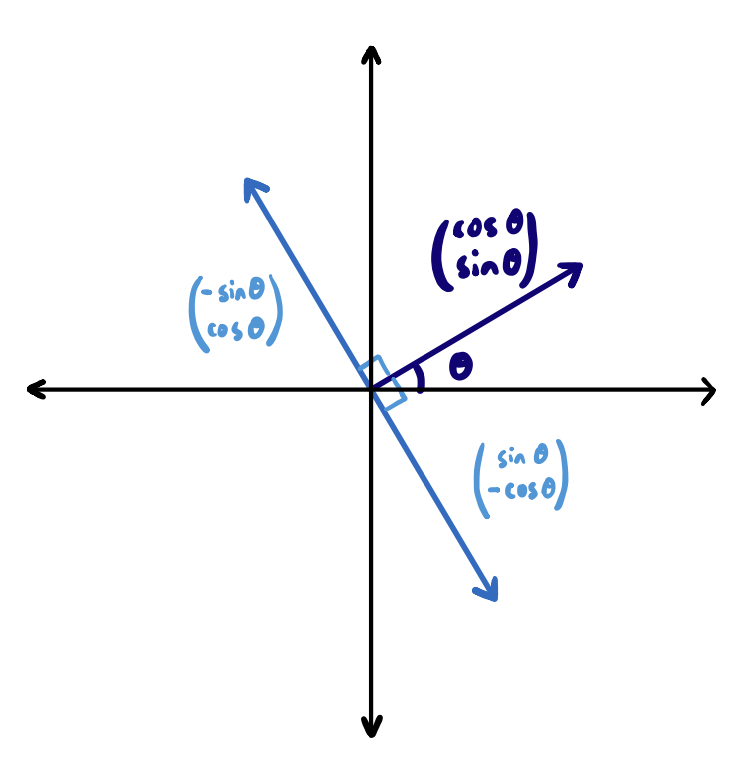
\includegraphics[width=8cm]{Lecture Files and Images/lec12-1.png}
\end{center}
\end{example}


In particular, the first type of matrix has determinant 1, and forms the subgroup $SO_n$, and the second has determinant $-1$ and forms its the non-trivial coset. Geometrically, the first type of matrix in $O_2$ are rotations by $\theta$ around the origin. The matrices of the second type, $A = \begin{pmatrix}
\cos \theta & \sin \theta \\
\sin \theta & -\cos \theta
\end{pmatrix},$ have characteristic polynomial $p_A(t) = t^2 - 1 = (t + 1)(t - 1)$. Thus, they have distinct eigenvalues $\pm 1,$ in contrast to rotation matrices, which do not have any real eigenvalues. Because the eigenvalues are distinct, there is an eigenbasis $\{\vec{v_+}, \vec{v_-}\}$.


\begin{theorem}
    The matrices of the second type are reflections across a line through the origin at an angle of $\theta/2$.
    
    \begin{center}
    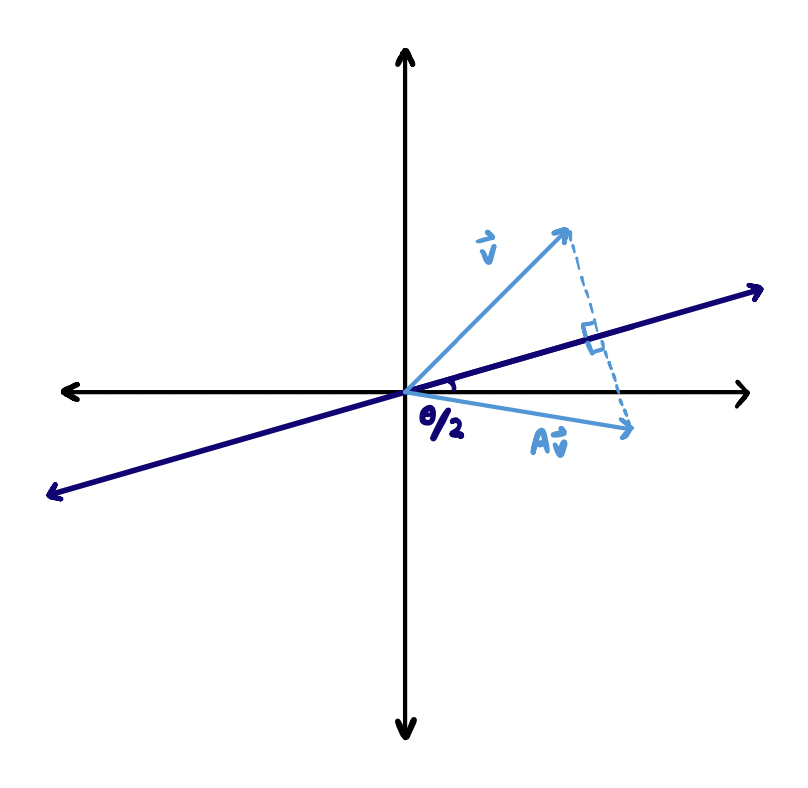
\includegraphics[width=7cm]{Lecture Files and Images/lec12-2.png}
\end{center}
\end{theorem}
\begin{proof}
Consider the line $L = \spann(\vec{v_+});$ since $\vec{v_+}$ is an eigenvector with eigenvalue 1, $A$ fixes this line. Notice that \[\vec{v_+} \cdot \vec{v_-} = A\vec{v_+} \cdot A \vec{v_-} = \vec{v_+} \cdot (-\vec{v_-}),\] where the first equality comes from the fact that $A$ is orthogonal, and the second comes from the eigenvalues $1$ and $-1$ of $v_+$ and $v_-$. The only possibility is $\vec{v_+} \cdot \vec{v_-}  = 0,$ so the two eigenvectors are orthogonal. Writing out any other vector in terms of the eigenvectors, $Av$ is precisely the reflection across $L$. 

\begin{center}
    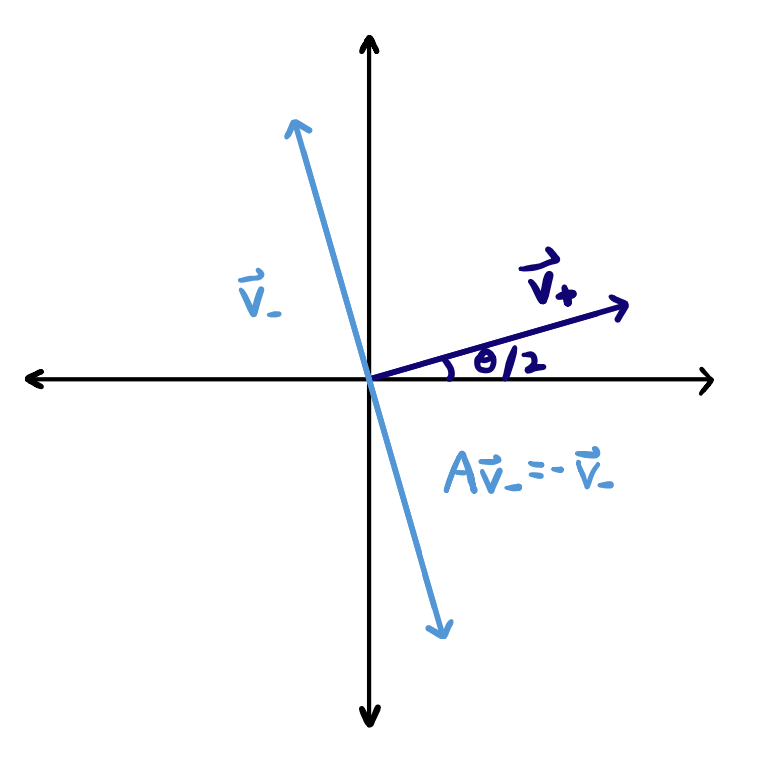
\includegraphics[width=7cm]{Lecture Files and Images/lec12-3.png}
\end{center}

\end{proof}

As expected, rotations and reflections preserve distance, and in fact they make up all the $2 \by 2$ orthogonal matrices. A fun fact that comes from this analysis is that the composition of two reflections over different lines will be a rotation, since the product of determinants will be $(-1)\cdot(-1) = 1.$ Orthogonal matrices can be thought of either geometrically or algebraically!

\subsection{Orthogonal Matrices in Three Dimensions}


In two dimensions, $SO_2$ consists of rotation matrices. It turns out that in three dimensions, $SO_3$ also consists of rotation matrices. 

In particular, a rotation in $\RR^3$ is characterized by the axis of the rotation, which is a unit vector $\vec{u} \in \RR^3$, and the angle of the rotation, which is some $\theta \in \RR.$
The plane \[u^{\perp} = \{v \in \RR^3: u \cdot v = 0\}\] consists of all the vectors in $\RR^3$ that are perpendicular to $\RR^3.$ 

\begin{center}
    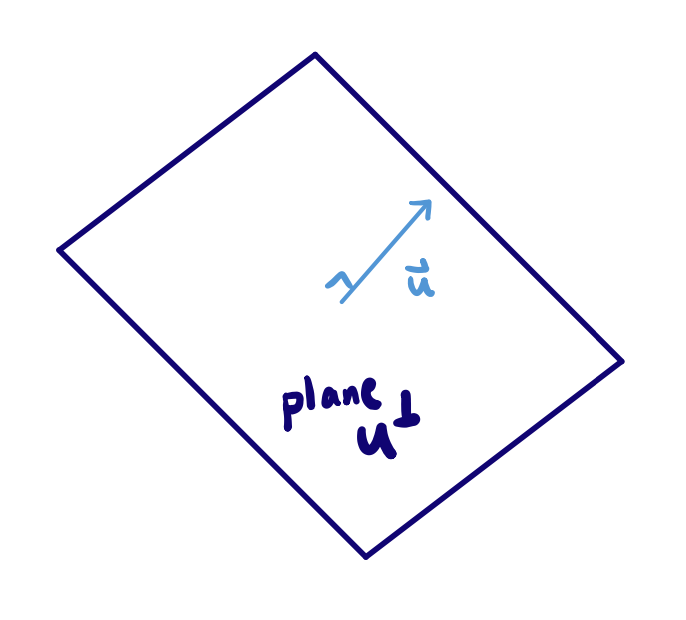
\includegraphics[width=7cm]{Lecture Files and Images/lec12-4.png}
\end{center}

\begin{definition}
The \textbf{rotation operator} with \textbf{spin labels} $u$ and $\theta$ is $\rho_{(u, \theta)},$ the linear operator $\rho: \RR^3 \rto \RR^3$ such that $\rho(u) = u$ and $\rho|_{u^{\perp}}$ is the rotation by $\theta$ counterclockwise with respect to the direction that $u$ points in.\footnote{Since every vector in $\RR^3$ is a linear combination of $u$ and some vector in $u^{\perp},$ the rotation operator is described completely by these conditions.}
\end{definition}

There is some redundancy in this description; for example, $\rho_{(u, \theta)} = \rho_{(-u, -\theta)}.$
\begin{theorem}
The rotation operators are exactly $SO_3$.
\end{theorem}
From geometric intuition, this result is not very surprising, since rotations preserve distance.\footnote{And orientation}
\begin{proof}

First, we show that all the rotation matrices are in $SO_3,$ and then we show that all matrices in $SO_3$ are rotation matrices.
\begin{itemize}
    \item  We first show that all of these rotation matrices belong to $SO_3$. Let $\{v, w\}$ be an orthonormal basis for the plane $u^\perp$, and let $P$ be a $3\times 3$ matrix with columns $(u,v,w)$. Since $v$ and $w$ are orthogonal to each other, and $u$ is orthogonal to both $v$ and $w,$ $P \in O_3.$ Conjugating a rotation matrix by $P$ demonstrates the action of $\rho_{(u, \theta)}$ with respect to the basis $(u, v, w).$ Since $u$ is fixed by the rotation matrix, the first column is $(1, 0, 0)^t,$ and since the plane $u^{\perp}$ is being rotated by $\theta,$ the rest of the matrix $M$ is given by the form of a $2 \by 2$ rotation matrix. That is,
    \[
    P^{-1}\rho_{(u, \theta)}P = \begin{pmatrix} 1 & 0 & 0 \\ 0 & \cos \theta & -\sin \theta \\ 0 & \sin \theta & \cos \theta \end{pmatrix} = M,
    \] which is in $SO_3.$ Since $\rho_{(u, \theta)} = PMP^{-1},$ and since $P, P^{-1} \in O_3$ and $M \in SO_3,$ the rotation matrix $\rho_{(u, \theta)}$ is also in $O_3.$ Taking the determinant of both sides\footnote{$\det(PMP^{-1}) = \det(P)\det(M)\det(P)^{-1} = \det(M) = 1$} demonstrates that $\rho_{(u, \theta)} \in SO_3.$
    
\item 
    To show the other direction, an element $A \in SO_3$ must be shown to be rotation around some axis $u,$ which has to be some eigenvector with eigenvalue $\lambda = 1$. There exists such an eigenvector if and only if $1$ is a root of the characteristic polynomial of $A,$ which is precisely when $\det(I-A) = 0.$
    
    Since $\det(A^T) = 1,$ $\det(A - I) = \det(A^T(A - I)).$ Using the fact that $A$ is orthogonal, this is $\det(I - A^T).$ Taking the transpose, this is $\det(I - A).$ Since the matrices are $3 \by 3,$ $\det(I-A) = (-1)^3\det(A-I).$
    Combining these,
    \begin{align*}
        \det(A-I) &= \det(A^T (A - I)) \\
                  &= \det(I - A^T) \\
                  &= \det(I-A) \\
                  &= (-1)^3 \det(A-I),
    \end{align*}
    implying that $\det(A-I) = 0.$ Therefore, there does exist an eigenvector of eigenvalue 1 for $A,$ which can be scaled to be a unit vector $u.$

    We extend $u$ to an orthonormal basis $P = (u, v, w)$ by picking an orthonormal basis for $u^\perp$. Consider taking $A$ in this basis. The first column is $(1, 0, 0)^t$, since $u$ is an eigenvector, and the first row is $(1, 0, 0)$ because the columns are orthogonal. Then, the bottom right submatrix is an element of $SO_2$ by taking the determinant. 
    So \[P^{-1} AP =
    \begin{pmatrix}
        1 & 0 & 0 \\
        0 & \cos & -\sin \\
        0 & \sin & \cos
    \end{pmatrix},
    \]
    and we are done.
\end{itemize}

\end{proof}

\newpage

\lhead{Lecture 13: Isometries}
\setcounter{section}{12}
%MIT OpenCourseWare: https://ocw.mit.edu
%RES.18-011 Algebra I Student Notes, Fall 2021
%License: Creative Commons BY-NC-SA 
%For information about citing these materials or our Terms of Use, visit: https://ocw.mit.edu/terms.

\section{Isometries}
\subsection{Review}
Last time, we discussed the orthogonal matrices $O_n$, which are matrices which preserve the dot product, which is a measure of length. We found that if we looked at the orthogonal matrices which had determinant 1, $SO_n,$ they actually turned out to be rotations in 2-space and 3-space! The rest of the orthogonal matrices $O_3$ can be obtained from $SO_3$ by multiplying a rotation matrix by 
\[
\begin{pmatrix}
-1 & & \\
& 1 & \\
& & 1
\end{pmatrix};
\]
the result will be a reflection over some axis. As a result, all length-preserving $3 \by 3$ matrices are rotations or reflections. 

\subsection{Isometries}

Without any prior knowledge, we might assume that there are many different types of length-preserving mappings, called isometries. We found that for linear mappings, the isometries were the orthogonal matrices, and two or three dimensions, they were rotations or reflection. What are the possibilities for isometries that are not linear?

\begin{qq}
Orthogonal matrices are the linear mappings that preserve distance. What are the other possibilities for distance-preserving mappings that are not necessarily linear?
\end{qq}

An isometry from $\RR^n$ to $\RR^n$ is a length-preserving mapping. 

\begin{definition}
A function $f: \RR^n \rto \RR^n$ is an \textbf{isometry} if 
\[
|f(u) - f(v)| = |u - v|
\]
for all $u, v \in \RR^n.$
\end{definition}

Let's take a look at two key examples.

\begin{example}
For a matrix $A \in O_n,$ the linear transformation 
\begin{align*}
\RR^n &\rto \RR^n \\
\vv{x} &\mapsto A\vv{x}
\end{align*}
is an isometry.
\end{example}


\begin{example}
Translation by a vector $\vv{v} \in \RR^n$ \footnote{This is \emph{not} a linear transformation!} is an isometry:
\begin{align*}
    \RR^n &\xrightarrow[]{t_{\vv{b}}} \RR^n \\
    \vv{x} &\mapsto \vv{x} + \vv{b}
\end{align*}
\end{example}

How crazy can an isometry be? The answer, fortunately or unfortunately, is \emph{not very}. In fact, these two examples and their compositions turn out to be the \emph{only} isometries. 

\begin{theorem}\label{isometry linear trans}
Every isometry $f$ is of the form $t_{\vv{b}}\circ A,$ for $A \in O_n$ and $\vv{b} \in \RR^n.$ So $f(\vv{x}) = A\vv{x} + \vv{b}.$
\end{theorem}

Despite the fact that preserving distance does not appear to be a very strong condition on $f$, it turns out that it is equivalent to the very strong condition that it basically has to be linear, combined with a shift. It boils down to the following lemma. What form do the isometries that fix the origin take? The answer is that they must be linear.

\begin{lemma}
If $f: \RR^n \rightarrow \RR^n$ is an isometry such that $f(0) = 0,$ it must be a linear transformation.\footnote{It must respect the additive and scalar multiplicative structure on $\RR^n$.} 
\end{lemma}

\begin{proof}

We must show that $f$ preserves sums and scalar products. First, we see that a dot product can be written in terms of $\vv{0}$ and distances:
    \[
    \vv{u} \cdot \vv{v} = \frac{1}{2}\left(|\vv{u} - \vv{0}|^2 + |\vv{v} - \vv{0}|^2 - |\vv{u}-\vv{v}|^2\right).
    \]
    
As a result, the following equation also holds:
    \[
    f(\vv{u}) \cdot f(\vv{v}) = \frac{1}{2}\left(|f(\vv{u}) - f(\vv{0})|^2 + |f(\vv{v}) - f(\vv{0})|^2 - |f(\vv{u})-f(\vv{v})|^2\right).
    \]
    
    Because $f$ is an isometry, $|a-b| = |f(a)-f(b)|$. Setting $f(0) = 0$ gives the equation $\vec{u} \cdot \vec{v} = f(\vec{u}) \cdot f(\vec{v}),$ so it must be the case that since $f$ preserves lengths, $f$ also preserves the dot product.
\begin{itemize}
    \item The sum can be expressed using a dot product again. For $\vv{z} = \vv{x} + \vv{y},$ 
    \[
    (\vv{z} - \vv{x}-\vv{y}) \cdot (\vv{z} - \vv{x}-\vv{y}) = 0,
    \]
    and so 
    \[
    \vv{z} \cdot \vv{z} + \vv{x} \cdot \vv{x} + \vv{y}\cdot\vv{y} - 2\vv{x}\cdot\vv{z} - 2\vv{y}\cdot \vv{z} + 2\vv{x}\cdot\vv{y} = 0.
    \]
    
    Now, since we know that addition is determined in some complicated way from dot product, since $f$ fixes the dot product, it must fix addition as well. \footnote{If we had some other crazy invented operation determined from the dot product, $f$ must also fix that!}
    So $f(z) = f(x) + f(y).$
    
    \item A similar reasoning gives us the scaling product: $f(cx) = cf(x).$
\end{itemize}

\end{proof}

Despite the fact that the only piece of information is that $f$ preserves distances and maps the origin to itself, it is enough to play around algebraically to find out that $f$ must be linear. This rules out lots of crazy functions that you could imagine could be isometries. 

\begin{proof}[Proof of Theorem \ref{isometry linear trans}]


Now, we can prove the original theorem. Given $f: \RR^n \rto \RR^n,$ there is some vector $b \in \RR^n$ such that $f(0) = b.$ Then $t_{-b} \circ f$ is an isometry that fixes $0.$ Thus, there is some linear transformation $A$ such that $t_{-b} \circ f = A,$ and this implies that $f = t_{b} \circ A,$ since $t_{b}$ is the inverse of $t_{-b}.$ From the definition of an isometry, it is easily seen that the composition of two isometries is an isometry.

\end{proof}

Given that isometries are all of the same restrictive form, it is not surprising that they form a group.

\begin{definition}
The \textbf{group of isometries} is
\[
M_n \coloneqq \{\text{isometries } \RR^n \xrightarrow[]{f} \RR^n\} \subseteq \text{Perm}(\RR^n).\footnote{Any bijective function on $\RR^n$ permutes the vectors in $\RR^n,$ since it maps each vector in $\RR^n$ to exactly one vector in $\RR^n,$ which is potentially itself.}
\]
\end{definition}

Clearly, translations, which are isomorphic to $(\RR^n, +),$ form a subgroup of $M_n,$ since $t_{\vv{b}} + t_{\vv{b'}} = t_{\vv{b}+\vv{b'}}$. Orthogonal matrices $O_n$ also form a subgroup of $M_n.$

Note that the composition of an orthogonal matrix with a translation is
\[
A\circ t_{\vv{b}} = t_{A\vv{b}} \circ A,
\]
since 
\[
A(x + b) = Ax + Ab. 
\]
In particular, a translation and an orthogonal matrix do \emph{not} commute with each other.

Consider the projection \begin{align*} \pi: &M_n \rto O_n \\
& t_b \circ A \mto A.\end{align*} 
It is a group homomorphism, since 
\[
(t_b \circ A) \circ (t_{b'} \circ A') = t_{b + Ab'} \circ AA'.
\]
Also, $\pi$ is surjective, and the kernel is $\ker(\pi)$, which are translations. Thus, the subgroup of translations is normal inside $M_n.$

\subsection{Isometries in 2-space}

Now that we have an understanding of isometries in general, let's narrow it down to an analysis in two dimensions.

\begin{qq}
For $n=2$, what do isometries look like?
\end{qq}

The following definition is an intuitive extension of the idea of orientation for linear mappings.

\begin{definition}
An isometry $x \mapsto Ax + b$ is \textbf{orientation-preserving} if $\det(A) = 1$, and \textbf{orientation-reversing} if $\det(A) = -1.$
\end{definition}

In two dimensions, isometries can be classified into one of four types.
\begin{theorem}\label{isometry four}
Every isometry on $\RR^2$ is 
\begin{enumerate}
    \item Translation
    \item Rotation around a point $p$\footnote{It is no longer required that $p$ is the origin, since the isometry does not have to be a linear transformation}
    \item Reflection across a line $L$ \footnote{Again, the line $L$ may or may not pass through 0; the isometry is not necessarily linear.}
    
    \begin{center}
        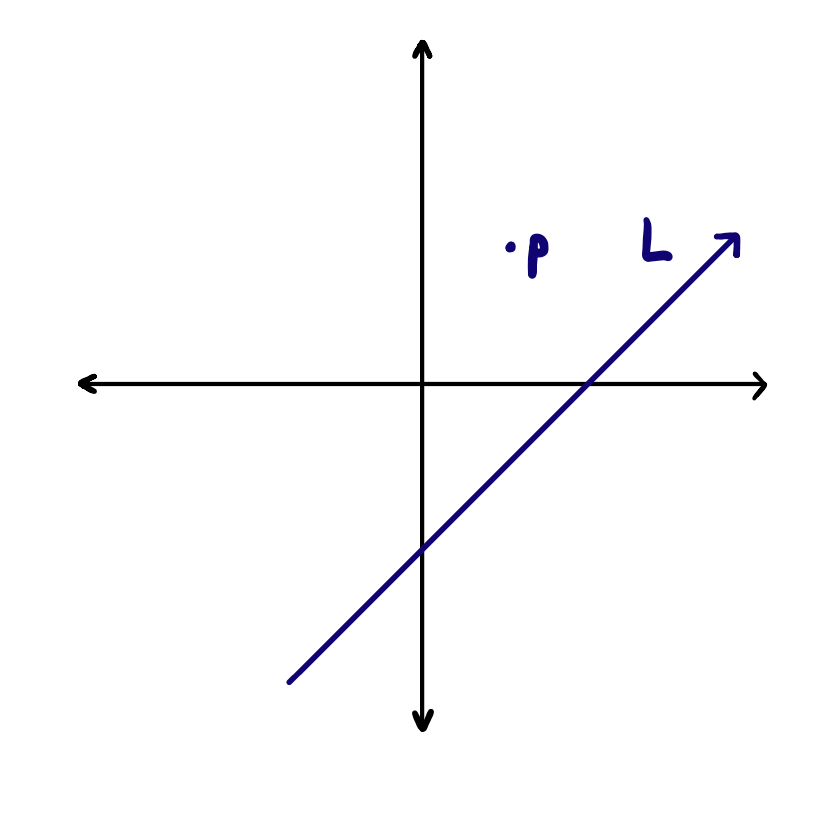
\includegraphics[width=5cm]{Lecture Files and Images/lec13-1a.png}
    \end{center}

    \item Glide reflection --- first, reflect across a line $L,$ then translate by some vector $b$ parallel to $L$\footnote{We will see diagrams next week which have glide reflections in their symmetry group!}
\end{enumerate}
\begin{center}
 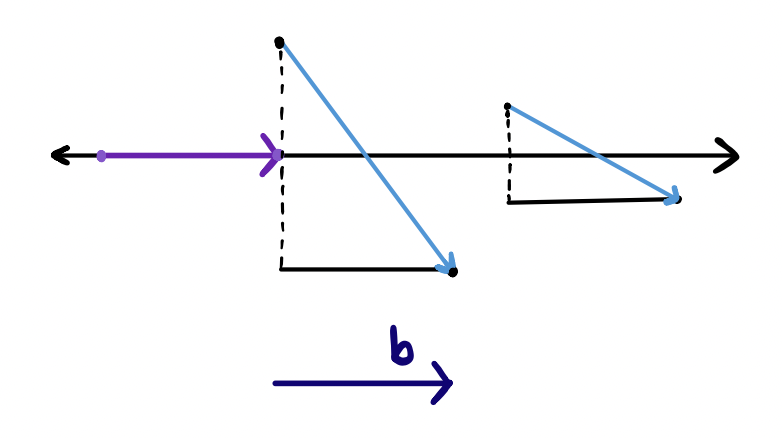
\includegraphics[width=5cm]{Lecture Files and Images/lec13-1b.png}
\end{center}
\end{theorem}

The first two are orientation-preserving; the last two are orientation-reversing. 

By composing with translations, it is possible to essentially change coordinate systems. For example, consider rotations and reflections. Let $f$ be an isometry, say a rotation around the origin. Then, 
\[
t_p f t_{-p}
\]
is a new isometry that fixes $p$, instead of the origin, since it is applying $f$ but after shifting coordinates by $p.$ \footnote{When we apply $t_{-p}$, we shift $p$ to 0, then we use $f$ to rotate around 0, and lastly use $t_p$ to shift $0$ back to $p.$} 

Similarly, letting $f$ be a reflection across any line, we can represent it in new coordinates as a reflection across a line through the origin. 

\begin{proof} We split the proof up into two cases depending on whether $f$ is orientation-preserving or reversing.
\begin{itemize}
    \item 
\textbf{Case I.}
Consider an orientation-preserving isometry $f(x) = A_{\theta}x + b.$  %37:16???

\begin{enumerate}
    \item If $A_{\theta} = I_2$, the identity, then $f = t_b,$ which is possibility 1 in the theorem.

    \item Otherwise, if $A_{\theta} \neq I_2,$ we want to find a fixed point $p$ such that $f(p) = p.$ Since $A_{\theta}$ has no fixed vectors, $p_A(1) \neq 0,$ and so $A_{\theta} - I_2$ has a trivial kernel, and so $A - I_2$ is invertible. Then the equation 
\[
(A-I_2) p = -b
\]
has a unique solution $p = (A-I_2)^{-1}(-b),$ and then 
\[
f(p) = Ap + b = p.
\]
So 
\[
t_{-p} A t_p = A_{\theta},
\]
since it fixes 0. This corresponds to the second possibility: rotation around a point $p.$
\end{enumerate}

\item \textbf{Case II.} 


Let $f$ be an orientation-reversing isometry. Then $f = t_b \circ A,$ where $A$ is reflection across a line $L.$ First, change the origin to $b/2.$ Then 
\[
t_{-b/2} f t_{b/2} = t_{-b/2} t_b A t_{b/2} = t_{b/2} t_{Ab/2} A = t_m A,
\]
where $m = \frac{b + Ab}{2}.$ Since $b$ and $Ab$ are reflections over a line $L,$ $m$, the average, must lie on that line. 
\begin{center}
    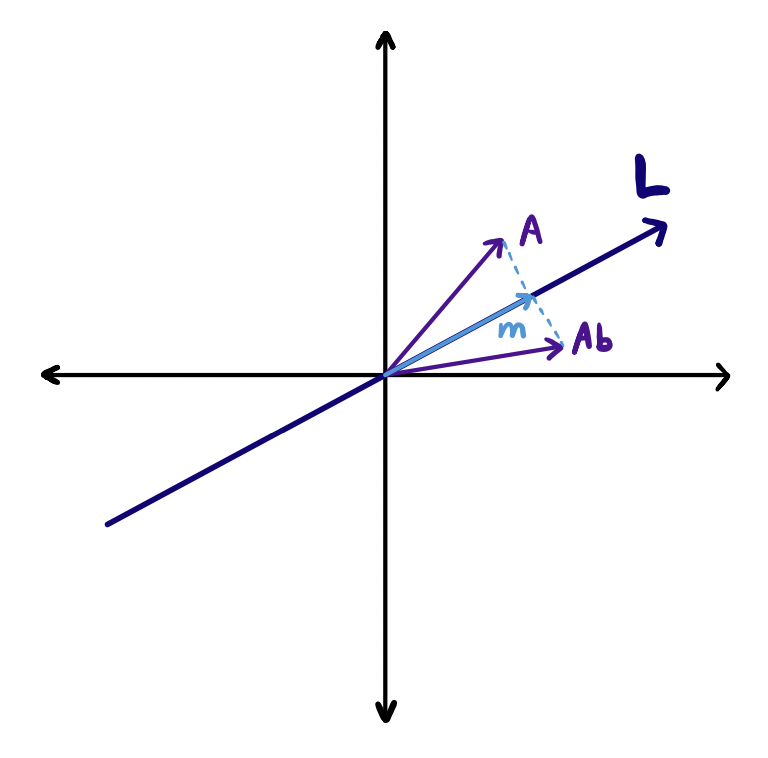
\includegraphics[width=8cm]{Lecture Files and Images/lec13-2alt.png}
\end{center}

\begin{enumerate}
    \setcounter{enumi}{2}
    \item If $m = 0,$ it is a reflection. 
    \item If $m \neq 0,$ it is a glide reflection. \footnote{In our proof, we try to be slicker about it, but if we are uncomfortable with that, we know $f$ is just $Ax + b,$ and we could simply crunch through lots of sines and cosines to force $f$ into one of the four forms in Theorem \ref{isometry four}.}

\end{enumerate}

Again, the same idea from Case I applies. Shifting to a new coordinate system gives us either a reflection or a glide reflection.

\end{itemize}

\end{proof}


\newpage

\lhead{Lecture 14: Finite and Discrete Groups of Isometries}
\setcounter{section}{13}
%MIT OpenCourseWare: https://ocw.mit.edu
%RES.18-011 Algebra I Student Notes, Fall 2021
%License: Creative Commons BY-NC-SA 
%For information about citing these materials or our Terms of Use, visit: https://ocw.mit.edu/terms.

\section{Symmetry Groups}

So far, in this class, we've covered \emph{groups} and \emph{linear algebra}. Now, we are looking at groups of symmetries that preserve extra forms of structure. 

\subsection{Review}
Last week, we looked at the \emph{orthogonal matrices}. 
 
\begin{definition}
The \textbf{orthogonal matrices} $O_n$ are matrices that preserve \emph{distance}. It is the set 
\[
T: \RR^n \rto \RR^n : |Tv| = |v| \text{ for all } v \in \RR^n.
\]
\end{definition}

\begin{definition}
The set $M_n$ of \textbf{isometries} from $\RR^n$ to itself is 
\[
\{f: \RR^n \rto \RR^n : |f(u)-f(v)| = |u-v|\}.
\]
\end{definition}

The orthogonal matrices are the subset of isometries that are \emph{linear transformations.} In class, we showed that every isometry $f$ is of the form $f(x) = Ax + b$ where $A \in O_n$ and $b \in \RR^n.$

Then, we looked at $O_2,$ the orthogonal matrices in two dimensions. There are two possibilities for a transformation in $O_2.$
\begin{itemize}
    \item Rotations around $0$: these have determinant 1 and are called $SO_2$. \footnote{The special orthogonal group}
    \item Reflections across a line through $\vv{0}$: these have determinant -1
\end{itemize}

Then the \emph{isometries} of two-dimensional space, $M_2,$ also fit into several categories.\footnote{This is quite surprising, since a priori, an isometry could take many different forms.}
\begin{itemize}
    \item Translations
    \item Rotations around $p$ 
    \item Reflections across a line
    \item A glide reflection\footnote{A reflection in addition to a parallel translation}
\end{itemize}

\subsection{Examples of Symmetry Groups}
Now, we want to add some additional structure to preserve.

\begin{qq}
What isometries of $\RR^2$ fix some shape inside $\RR^2$?
\end{qq}

We call the group of such isometries \emph{symmetry groups} for that shape. Let's start with a couple examples of shapes and their symmetry groups. 
\begin{example}
For a regular pentagon, the group of symmetries are rotations by multiples of $\frac{2\pi}{5}$, and reflections across lines. This group of symmetries is what we would call \emph{discrete}.\footnote{This will be formalized later on.}
\begin{center}
    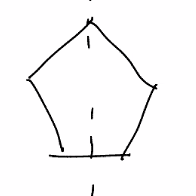
\includegraphics[width=3cm]{Lecture Files and Images/lec14-pentagon.png}
\end{center}
\end{example}
Next, we look at a group that is not discrete.
\begin{example}
For a circle centered at the origin, every rotation or reflection will fix it, and so its symmetry group is all of $O_2.$ This group of symmetries is \emph{not discrete}.
% \begin{center}
%     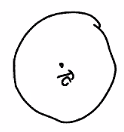
\includegraphics[width=3cm]{images/lec14-circle.png}
% \end{center}  %\todo put the graphics back in
\end{example}
We can also look at infinitely large shapes. 
\begin{example}
For a triangular lattice, certain translations, reflections over lines, rotations, and glide reflections all preserve it. It is a \emph{discrete} symmetry group.
\begin{center}
    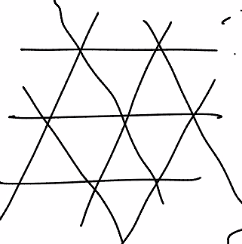
\includegraphics[width=3cm]{Lecture Files and Images/lec14-trianglelattice.png}%\todo add in picture of glide reflection from lecture notes
\end{center}
\end{example}

\subsection{Discrete Subgroups of \texorpdfstring{$\RR$}{R}}
From our examples, we see that some symmetry groups are ``discrete" and some are not.
\begin{qq}
How can the notion of a \emph{discrete group} be formalized?
\end{qq}
We can start with an easier notion, which is a discrete group inside $(\RR, +).$
\begin{definition}
A group $G \leq (\RR, +)$ is discrete if there exists $\varepsilon > 0$ such that any $g \in G$ such that $g \neq 0$ satisfies $|g| > \varepsilon.$ Equivalently, for $a, b \in G$ and $a \neq b,$ then it must be true that $|a-b| > \varepsilon$ for a discrete group. 
% \begin{center}
%     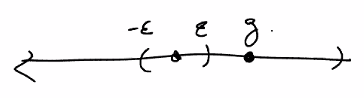
\includegraphics[width=3cm]{images/lec14-discrete.png}
% \end{center} %\todo{put the graphics back in}
\end{definition}

The discreteness tells us some important information about $G.$
\begin{theorem}\label{discrete subgroups of r}
If $G \leq (\RR, +)$ is discrete, then $G = \{0\}$ or $G = \ZZ \alpha$ for some real number $\alpha > 0.$ 
\begin{center}
    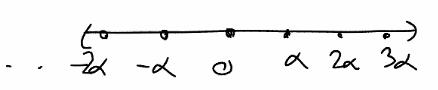
\includegraphics[width=5cm]{Lecture Files and Images/lec14-disc.png}
\end{center} %\todo put the graphics back in
\end{theorem}
This theorem is very similar to the theorem we had about subgroups of $\ZZ,$ where we showed they were either trivial or of the form $k\ZZ$.
\begin{proof}
Assume that $G \neq \{0\}.$ Then there is some smallest positive element $\alpha \in G.$ 
To see why it is possible to find a smallest element, we start by taking any $g > 0$ in $G$. 
By discreteness, in the interval from $[0, g]$, we have at most $g/\varepsilon$ elements of $G$ inside of the interval. 
We can then pick the smallest one because the set is finite.

We now claim that $G = \ZZ \alpha.$ Why is this true? If $2\alpha < x < 3\alpha$ for some $x \in G,$ then $0 < x-2\alpha < \alpha,$ where $x-2\alpha \in G,$ which is a contradiction.
\footnote{The discreteness guarantees that we can find a smallest positive element! This is definitely \emph{not} the case for $\RR$ in general (it is a fundamental property of $\RR$ that there is \emph{no} smallest positive element.)}
\end{proof}

\subsection{Finite subgroups of \texorpdfstring{$O_2$}{O2}}
So what are all the finite subgroups of $O_2?$ 
Let's first try to create some examples to get some intuition about them.
\begin{example}
Let $x$ be a rotation by $\frac{2\pi}{n}.$ Then $C_n = \langle x \rangle$\footnote{$\{1, x, \cdots, x^{n-1}\}$}, the cyclic group of order $n,$ is generated by $x$, and is a finite subgroup of $O_2.$ 
\end{example}

Another possible finite subgroup can be created by expanding $C_n$ a little bit. 
\begin{example}
Let $y$ be a reflection across a line $\ell$ through $\vv{0}.$ Notice that the relations $yx = x^{-1}y, y^2 = e,$ and $x^n = e$ hold, and so any product  $y^{a_1}x^{a_2}y^{a_3}\cdots$ can be written as $x^{i}y^{j},$ where $0 \leq i < n$ and $0 \leq j < 2.$ Then the group generated by $x$ and $y$ is 
\[
D_n \coloneqq \langle x, y \rangle = \{e, x, x^2, \cdots, x^{n-1}, y, xy, x^2y, \cdots, x^{n-1}y\},
\]
which is called the dihedral group. It has order $2n.$
\end{example}

For $n \geq 3,$ $D_n$ is the group of symmetries of a regular $n-$gon.\footnote{In general, if $x$ is a rotation by an angle that is not a rational multiple of $2\pi,$ then we do not get a rational group. We would get a non-discrete subgroup of $SO_2.$} The dihedral group for $n= 1$ is $D_1 \cong C_2$ and for $n = 2$, $D_2 \cong C_2 \by C_2.$ For $n=3,$ $D_3 \cong S_3,$ and larger dihedral groups can also be studied. 

Now, we have two families of finite subgroups of $O_n$, the cyclic groups of rotations, and the dihedral groups. It turns out that these are actually all the finite subgroups of $O_2$. This provides yet another classification theorem.

Let's start with a simpler version. 
\begin{theorem}
If a subgroup $H \leq SO_2$ is finite, then $H$ is isomorphic to $C_n$ for some $n.$
\end{theorem}
\begin{proof}
Let $\rho_{\theta}$ be $\begin{pmatrix}
\cos\theta & -\sin\theta \\
\sin\theta & \cos\theta
\end{pmatrix}$. Then let
\[
S = \{\theta \in \RR \text{ such that } \rho_{\theta} \in H\}.
\]

Under the homomorphism $\pi: \theta \mapsto \rho_{\theta}$, $S = \pi^{-1}(H).$ Since $S$ is a preimage, we know that $S$ is a subgroup of $(\RR, +)$.

If $H$ is finite, then $S$ must be discrete, and so by Theorem \ref{discrete subgroups of r}, $S$ is $\ZZ \alpha$ for some $\alpha.$ Also, $2\pi \in S$ because a rotation by $2\pi$ is the identity in $H$, and so $\alpha = \frac{2\pi}{n}$. So $\boxed{H= C_n.}$ 
\end{proof}

\begin{theorem}\label{everything is cn or dn}
Any finite subgroup of $O_2$ is isomorphic to $C_n$ or $D_n.$ 
\end{theorem}
Now, we can prove Theorem \ref{everything is cn or dn}. 
\begin{proof}
There are two cases:
\begin{itemize}
    \item \textbf{Case I.} If $G \subseteq SO_2,$ by the above theorem, $G \cong C_n$ for some $n.$
    \item \textbf{Case II.} If $G$ is not a subset of $SO_2,$, then take the restriction of the determinant function on $O_2$ to $G.$ It takes \[G \xrightarrow[]{\det}\{\pm 1\}.\] By the assumption that $G$ isn't a subset of $SO_2,$ this is surjective. Let 
    \[
    H = \ker(G \xrightarrow[]{\det}\{\pm 1\}).
    \]
    Then, $H \nsub G$ is a normal subgroup of index 2. So $\det^{-1}(\{-1\})$ is a nontrivial coset of $H,$ and so it is $Hr$ for some $r \in G$ such that $\det(r) = -1.$ Then $r$ must be a reflection across some line $\ell.$\footnote{Note that we have many options for $\ell$ because any $r\in Hr$ generates $Hr$. In particular, these are all the rotations of $\ell$.} Then, it is clear by definition that $H \leq SO_2,$ and so $H = C_n$ for some $n,$ and it is generated by some $x = \frac{2\pi \rho}{n}$, and then we have 
    \[
    G = \left \langle \frac{2\pi\rho}{n}, r\right \rangle \cong D_n.
    \]
\end{itemize}
\end{proof}

\subsection{More Discrete Subgroups}
Next, what are the finite or discrete subgroups of $M_2$? Let's start with a couple of definitions. 

\begin{definition}
A subgroup $G \leq O_2$ is \textbf{discrete} if there exists some $\varepsilon > 0$ such that all nontrivial rotations in $G$ have angle $\theta$ such that $|\theta| > \varepsilon.$\footnote{Here, discrete implies finite, which implies that it is $C_n$ or $D_n.$}
\end{definition}

\begin{definition}
A subgroup $G \leq M_2$ is \textbf{discrete} if there exists some $\varepsilon > 0$ such that all translations in $G$ are by vectors $b$ with $|b| > \varepsilon,$ and all rotations in $G$ have angle $\theta$ such that $|\theta| > \varepsilon.$
\end{definition}

This ends up being quite a strong constraint on what the discrete subgroups look like, even though there could be lots of different possibilities. We'll talk about this more next time.

\newpage

\lhead{Lecture 15: Finite and Discrete Subgroups, Continued}
\setcounter{section}{14}
%MIT OpenCourseWare: https://ocw.mit.edu
%RES.18-011 Algebra I Student Notes, Fall 2021
%License: Creative Commons BY-NC-SA 
%For information about citing these materials or our Terms of Use, visit: https://ocw.mit.edu/terms.

\section{Finite and Discrete Subgroups, Continued}

\subsection{Review}
Last time, we began studying certain subgroups of $M_2.$ The group of \emph{isometries} of $\RR^2$ is precisely
\[
M_2 = \{t_{\vv{b}} \circ A : \vv{b} \in \RR^2, A \in O_2\},
\]
where $O_2$ is the group of orthogonal matrices. 

\begin{qq}
What are the finite subgroups of $O_2$?\footnote{The discrete subgroups of $O_2$ turn out to be the same as the finite subgroups, either $C_n$ or $D_n$ (we omit the proof, as it is in the homework.)} 
\end{qq}
One way in which subgroups of $M_2$ naturally arise is with symmetries of plane figures. 
\begin{example}
For the following two plane figures, they both have discrete symmetries including translations, rotations, and glide reflections. 
\begin{center}
    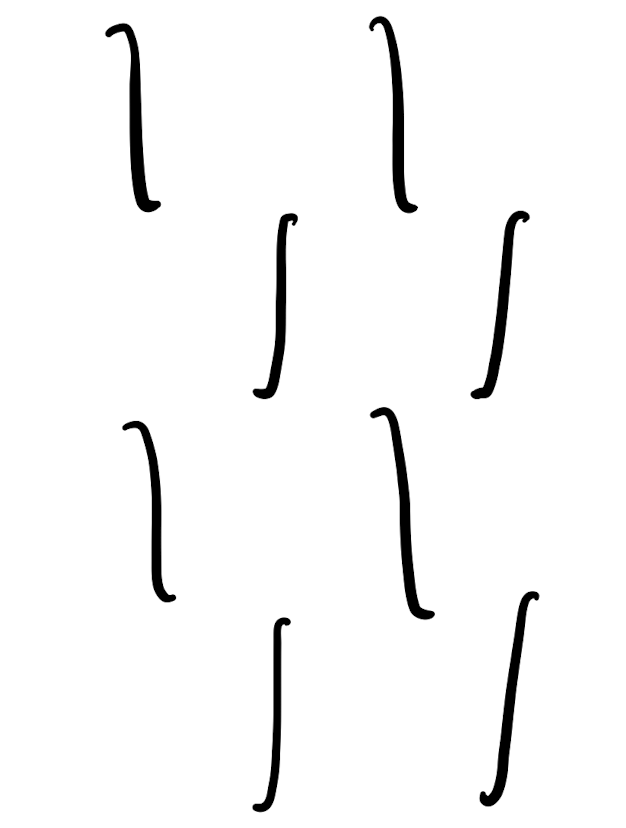
\includegraphics[width=3cm]{Lecture Files and Images/lec15-1integrals.png} 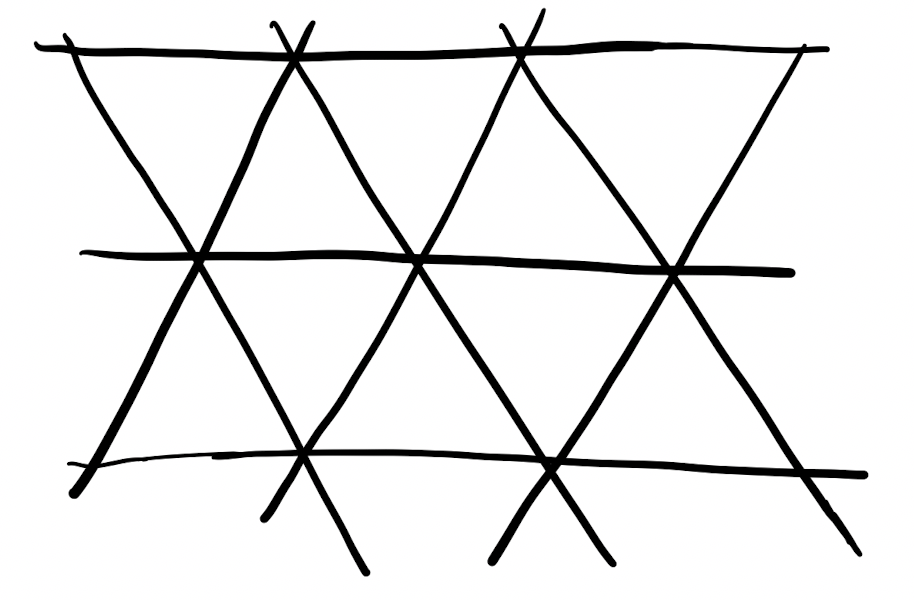
\includegraphics[width=6cm]{Lecture Files and Images/lec15-2trianglegrid.png}
\end{center}
\end{example}

Last time, we looked at finite subgroups of the orthogonal matrices $G \subseteq O_2.$ We found the following theorem which greatly restricts the possibilities for such subgroups:
\begin{theorem}\label{everything is cn or dn}
Any \emph{finite} subgroup $G \subseteq O_2$ is either 
\begin{itemize}
    \item $G \cong C_n = \langle \rho_{2\pi/n} \rangle$, the cyclic group generated by a \emph{rotation} by $2\pi/n$; or
    \item $G\cong D_n = \langle \rho_{2\pi/n}, r \rangle $ which is the group $C_n$ with an extra reflection $r.$  
\end{itemize}
\end{theorem}

The elements of the form $\rho_{2\pi/n}$, which are rotations by $2\pi/n,$ are orientation-preserving, while elements of the form $\rho_{2\pi / n}r$, which are reflections over certain lines through the origin, are orientation-reversing.


\subsection{Finite Subgroups of \texorpdfstring{$M_2$}{M2}}

Now that we have found the finite and discrete subgroups of $O_2,$ we bring our attention to finite subgroups $G \subseteq M_2.$
\begin{qq}
What are the finite subgroups of $M_2$? Do we get more subgroups now that we have more elements?
\end{qq}

In fact, there are \emph{no} new finite subgroups obtained from allowing $G$ to be in $M_2$ instead of $O_2.$ 

\begin{theorem}
Any finite subgroup $G \subseteq M_2$ is also isomorphic to $C_n$ or $D_n.$
\end{theorem}

\begin{proof}
In order to show that $G$ is isomorphic to $C_n$ or $D_n$, it is enough to find $s_0 \in \RR^2$ such that $g(s_0) = s_0$ for all $g \in G.$ Then, by changing coordinates such that $s_0$ is the new origin\footnote{We take $t_{-s_0}Gt_{s_0}$}, $G$ fixes the origin (formerly $s_0$) and so $G \subseteq O_2.$ As a result, by applying Theorem \ref{everything is cn or dn}, $G$ must in fact be isomorphic to $C_n$ or $D_n.$

\begin{itemize}
    \item \textbf{Step 1.} First, we find some finite set $S$ fixed by every element $g$: we require that $gS = S$ for all $g \in G.$ For any $p \in \RR^2,$ let 
    \[
    S = \{g(p) \in \RR^2: g \in G\}\footnote{This is called the \emph{orbit} of $p,$ since it is all the points that $p$ can reach by some transformation in $G$, or all the points that $p$ orbits to.}.%somehow this doesn't seem right in wording
    \]
    
    Then, for any element $s \in S,$ it is equal to $s = g'(p)$ for some $g' \in G,$ by the definition of $S.$ In addition, for any $g \in G,$ the action of $g$ on $s$ is
    \[
    g(s) = g(g'(p')) = (gg')(p) \in S,
    \]
    again by how $S$ is defined. So 
    \[
    gS = S.
    \]
    
    \item \textbf{Step 2.} Intuitively, to find $s_0,$ we would take the average, or the center of mass, of all the points. For example, for the set of rotations $\langle 2\pi/3\rangle,$ $S$ would be 3 equidistant points, and the center of the equilateral triangle would be fixed by such rotations. 
    From this intuition, we can apply the following averaging trick. This is where $G$ being finite is required, as we wouldn't be able to take the average otherwise. %ask davesh more about averaging to put in a footnote?
    
    Where $S = \{s_1, \cdots, s_n\}$, let
    \[
    s_0 = \frac{1}{n}(s_1 + \cdots + s_n)
    \]
    be the average of all the elements in $S.$ For any isometry $f = t_b \circ A,$ 
    \begin{align*}
    f(s_0) &= t_b\left(\frac{1}{n}(As_1 + \cdots + As_n)\right) \\
    &= \frac{1}{n}((As_1 + b) + \cdots + (As_n + b)) \\
    &= \frac{1}{n}(f(s_1) + \cdots + f(s_n)),
    \end{align*}
    since $A$ is a linear operator.
    
    As a result, for any $g \in G,$ 
    \begin{align*}
    g(s_0) &= \frac{1}{n}(g(s_1) + \cdots + g(s_n)) \\
    &= \frac{1}{n}(s_1 + \cdots + s_n) \\
    &= s_0,
    \end{align*}
    since $g$ permutes the elements in $S$.%why does it do that again lmao
    
    So we see that $G$ does fix $s_0,$ and by changing coordinates so that $s_0$ is the origin, $G$ must in fact be isomorphic to $C_n$ or $D_n.$
\end{itemize}
\end{proof}

\subsection{Discrete Subgroups of \texorpdfstring{$M_2$}{M2}}

No new finite subgroups are obtained by taking elements in $M_2$ instead of $O_2;$ what if we take discrete subgroups\footnote{We will formalize the notion of discreteness in $M_2$ now!} instead of finite subgroups? 

\begin{qq}
What about discrete subgroups of $M_2$? 
\end{qq}

The definition of discreteness in $M_2$ combines the two definitions for the rotations and translations.
\begin{definition}
A group $G \subseteq M_2$ is discrete if there exists some $\varepsilon > 0$ such that any translation in $G$ has distance $\geq \varepsilon$ and any rotation in $G$ has angle $\geq \varepsilon.$\footnote{In fact, for discreteness, it would make more sense to require two different $\varepsilon_1$ and $\varepsilon_2$ for translations and rotations, just to ensure that there are not continuously many translations and rotations. In this case, we can simply acquire the $\varepsilon$ for this definition by taking the minimum of the two; then any translation in $G$ has distance $\geq \varepsilon_1 \geq \varepsilon$ and any rotation has angle $\geq \varepsilon_2 \geq \varepsilon.$}

\begin{center}
    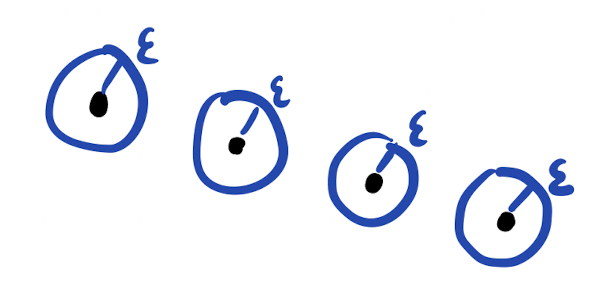
\includegraphics[width=5cm]{Lecture Files and Images/lec15-balls.png}
\end{center}
\end{definition}


\subsubsection{Discrete Subgroups of \texorpdfstring{$\RR^2$}{R2}}

As a warmup, let's consider the copy of the plane inside $M_2,$ $(\RR^2, +) \subseteq M_2,$ consisting of the translations $t_b.$ What are the discrete subgroups of $(\RR^2, +)$? The result and argument is similar to the discrete subgroups of $(\RR, +)$ that we covered last week. 

\begin{theorem}\label{discrete sub of r2}
If $G \subseteq \RR^2$ is discrete, then 
\begin{enumerate}
    \item G = \{0\}; or
    \item there exists some $\vec{\alpha} \in \RR^2$ such that $G = \ZZ \vec{\alpha};$ or
    
\begin{center}
    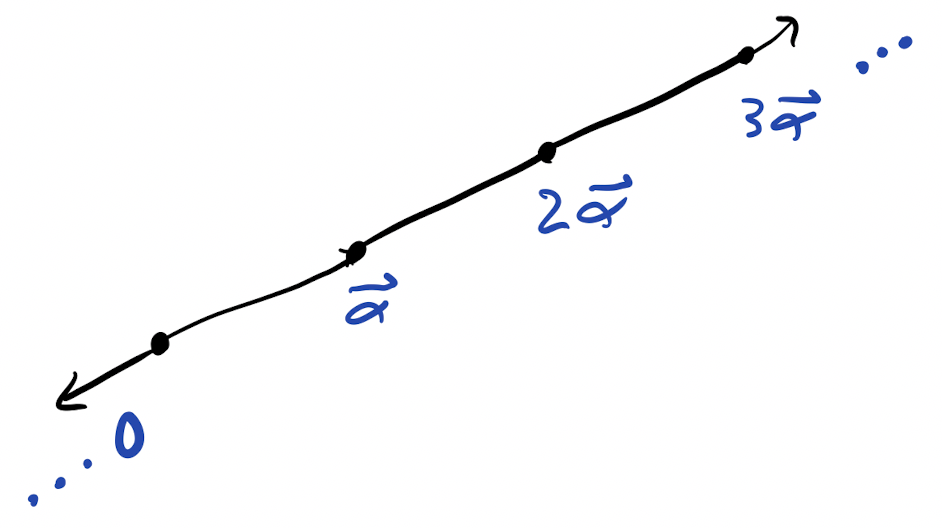
\includegraphics[width=5cm]{Lecture Files and Images/lec16-line.png}
\end{center}
    \item there exist linearly independent vectors $\vec{a}, \vec{b} \in \RR^2$ such that $G = \ZZ \vec{a} + \ZZ \vec{b}.$ This is called a \emph{lattice} inside $\RR^2.$
\begin{center}
    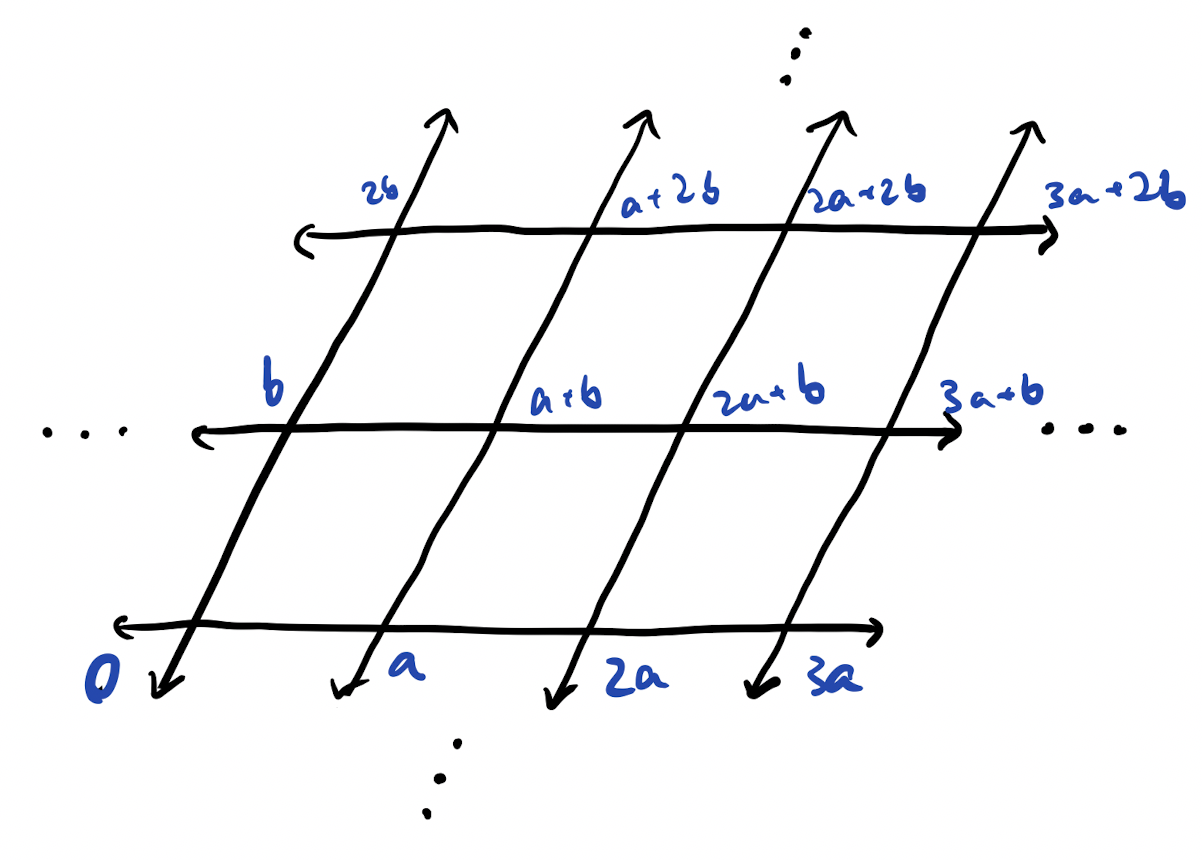
\includegraphics[width=5cm]{Lecture Files and Images/lec15-lattice.png}
\end{center}
\end{enumerate}
\end{theorem}

\begin{proof}
First pick any $\hat{\alpha} \neq 0 \in G.$ The intersection $G \cap \RR\hat{\alpha}$ must be discrete, so there is some smallest length vector in $G \cap \RR\hat{\alpha}$; call it $\alpha.$ Then if $G \cap \RR\hat{\alpha} = G,$ then $G \cap \RR\hat{\alpha} = \ZZ\alpha,$ and we are done. %why is this true?

Otherwise, pick $\beta \in G$ such that $\beta \notin \RR\alpha$, minimizing the distance from $\beta$ to $\RR\alpha.$ There exists such a $\beta$ because in any bounded region of $\RR^2,$ there can only be finitely many points of $G;$ then we can simply pick the point in $G$ closest to $\RR\alpha.$ 

\textbf{Claim: $G = \ZZ\alpha + \ZZ\beta.$} If this were not true, then there would exist a point $\gamma \in G$ that is not on the lattice formed by $\alpha$ and $\beta.$ Thus, by shifting by $\alpha$ and $\beta,$ the parallelogram with sides $\alpha$ and $\beta$ would contain a point closer to $\RR\alpha$, violating the minimality of $\beta$. 
\end{proof}

\subsubsection{Back to Discrete Subgroups of \texorpdfstring{$M_2$}{M2}!}

Now that we have considered the translations in $M_2,$ which are isomorphic to the plane $\RR^2,$ we can move on to the entire $M_2.$
\begin{qq}
How can we study discrete groups $G \subseteq M_2$?
\end{qq}

Recall that there exists a projection $\pi$ from $M_2$ to $O_2$, where $\RR^2,$ the group of translations, is the kernel. The projection takes 
\begin{align*}
    \ker(\pi) = \RR^2 \hookrightarrow\footnote{This arrow often denotes an inclusion map.} &M_2 \xrightarrow[]{\pi} O_2 \\
    &t_{\vv{b}} \circ A \mapsto A.
\end{align*}

The restriction of $\pi$ to $G$ takes $\pi|_G: G \rto O_2.$ The kernel $L = \ker(\pi|_G)$ consists of the translations in $G.$ Under this map, the image of $G$ is a subgroup $\overline{G} \coloneqq \pi(G) \subseteq O_2,$ known as the \textbf{point group} of $G.$ The projection takes
\[
\ker(\pi|_G) = L \subseteq G \xrightarrow[]{\pi|_G} \overline{G}.
\]

\begin{example}
For this infinite plane figure, the group of translations $L$ in the symmetry group $G$ is a rectangular lattice. The point group $\overline{G}$ contains rotation by $\pi$ around $\vv{0}$ and reflection across $\ell;$ as a result, $\overline{G}$ is isomorphic to $D_2.$ 

\begin{center}
    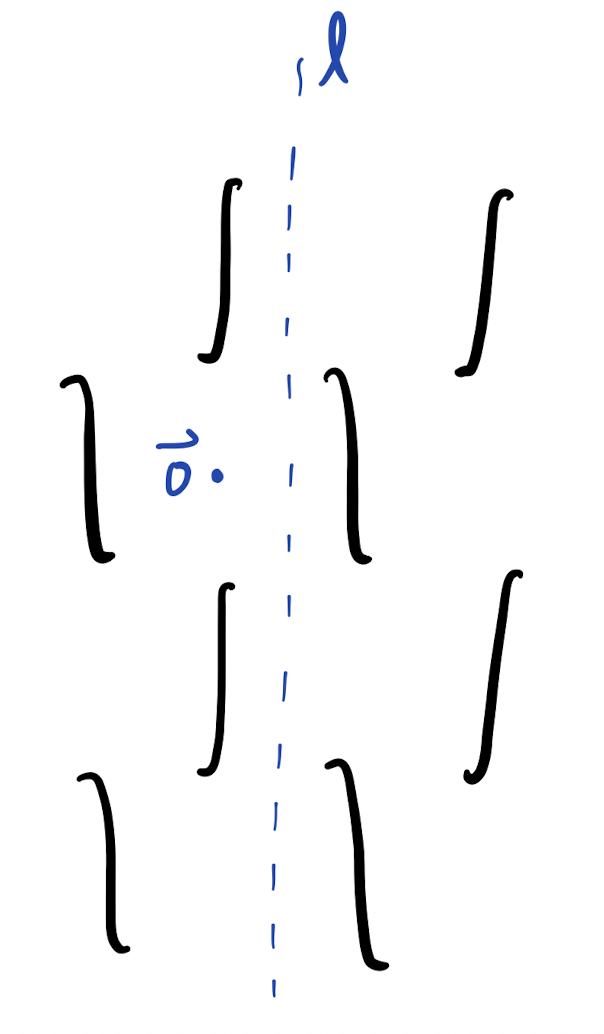
\includegraphics[width=3cm]{Lecture Files and Images/lec15-intl.png}  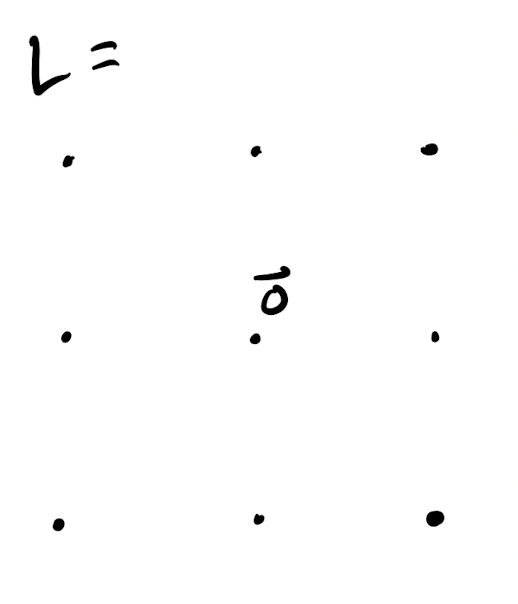
\includegraphics[width=4cm]{Lecture Files and Images/lec15-L0.png}
\end{center}
\end{example}

As we can see in the example, by using the projection $\pi,$ each $G$ can be decomposed into a discrete point group $\overline{G}$ isomorphic to $C_n$ or $D_n$, and a discrete group $L \subseteq \RR^2$, classified in Theorem \ref{discrete sub of r2}. In fact, we can constrain the possibilities even more! The following proposition is a start.

\begin{proposition}
Every $A \in \overline{G}$ maps $L$ to $L.$
\end{proposition}
\begin{proof}
Next time!
\end{proof}

%add another example?

\newpage

\lhead{Lecture 16: Discrete Groups}
\setcounter{section}{15}
%MIT OpenCourseWare: https://ocw.mit.edu
%RES.18-011 Algebra I Student Notes, Fall 2021
%License: Creative Commons BY-NC-SA 
%For information about citing these materials or our Terms of Use, visit: https://ocw.mit.edu/terms.

\section{Discrete Groups}
\subsection{Review}
Last time, we looked at discrete\footnote{The translations and rotations that cannot be arbitrarily small}  subgroups $G \leq M_2.$ Then, we looked at a projection $\pi$:
\begin{align*}
    \ker(\pi) &= (\RR^2, +) \subset M_2 \xrightarrow[]{\pi} O_2, \\
    t_b \circ A &\mapsto A;
\end{align*}
essentially, it gets rid of the translation part of an isometry. %Where $L$, the group of translations in $G,$ which is the symmetry group of $G,$, with the restriction of $\pi$ to $G,$ we get 

We can restrict $\pi$ to $G$ to get a mapping 
\[
G \xrightarrow[]{\pi|_G} O_2,
\]
and we call the kernel, 
\[
L \coloneqq \ker(\pi|_G),
\]

and it consists of all the translations in $G.$



%\[
%L \subset G \xrightarrow[]{\pi|_G} \overline{G} \coloneqq \pi(G),
%\]

The image of $G$ in $O_2$, denoted $\overline{G} \coloneqq \pi(G),$ is called the \emph{point group} of $G.$ For some element $g \in G,$ its image $\overline{g} \coloneqq \pi(g) \in \overline{G}$ only "remembers" the angle of rotation or the slope of the reflection line.

If $\overline{G}$ is discrete, it is either $C_n$ or $D_n,$ which we proved earlier.


If $L \subseteq \RR^2$ is discrete, then we obtained three possible cases. 
\begin{enumerate}[label = (\roman*)]
    \item $L = \{0\}$;
        \begin{center}
    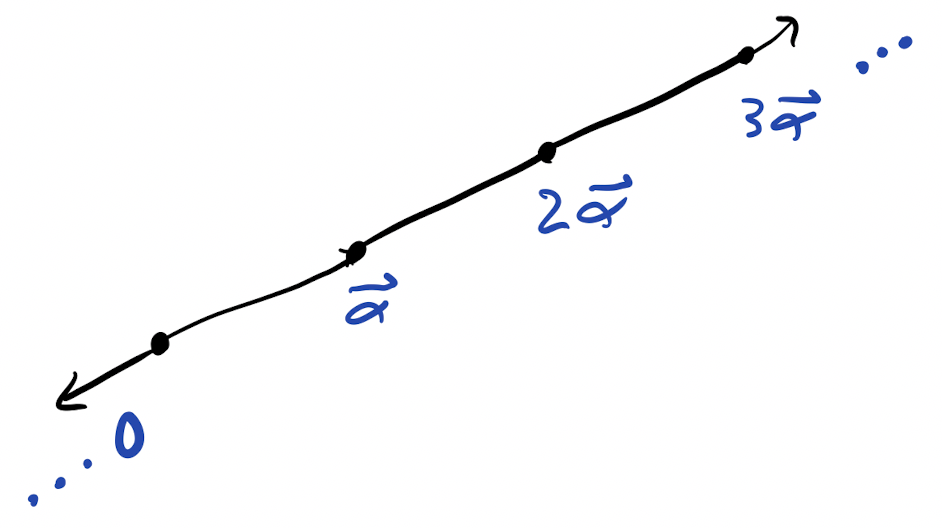
\includegraphics[width=6cm]{Lecture Files and Images/lec16-line.png}
\end{center}
    \item $L = \ZZ \alpha$ where $\alpha \neq 0;$
    \begin{center}
    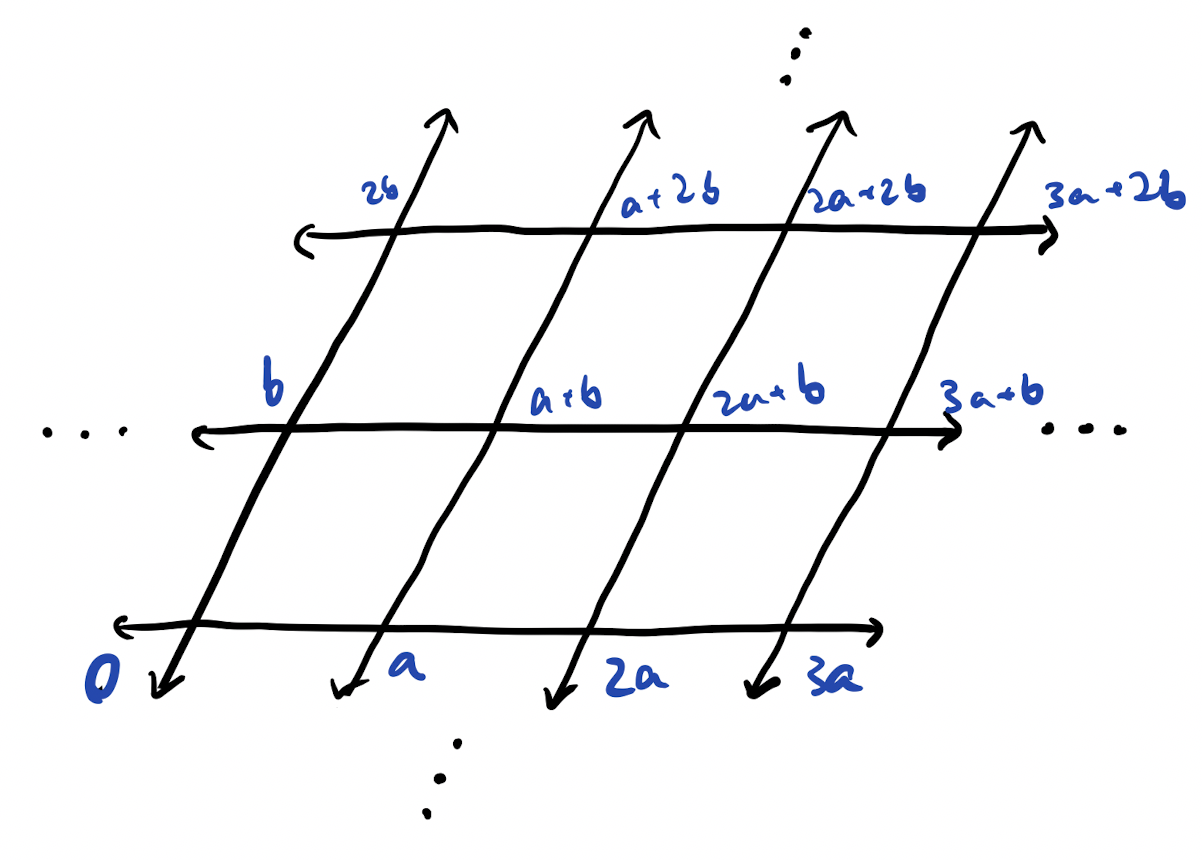
\includegraphics[width=6cm]{Lecture Files and Images/lec15-lattice.png}
\end{center}

    \item $L = \ZZ\alpha + \ZZ\beta$, where $\alpha, \beta$ are linearly independent.\footnote{When you look at two vectors and everything you generate from them, it's called a lattice.}%edit this 
    

\end{enumerate}

\subsection{Examples for \texorpdfstring{$L$}{L} and \texorpdfstring{$\overline{G}$}{G}}\label{examples for l and g}

For a given plane figure, it is actually not difficult to see what $L$ and $\overline{G}$ are! For the translation subgroup $L$, since it must either be the identity translation, $\ZZ\alpha$, or a lattice, it is possible to simply eyeball which translations preserve the figure. Let's consider the following plane figures. Later in this lecture, we will discuss the possibilities for $\overline{G}$; it consists of the (untranslated) rotations and reflections preserving a figure.




\begin{center}
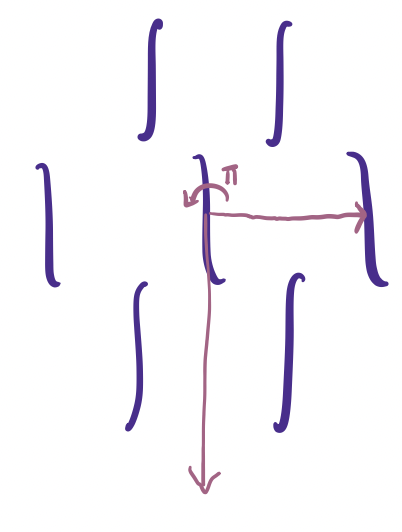
\includegraphics[width=4cm]{Lecture Files and Images/lec16-integrals.png}
\end{center}

\begin{example}[A]\label{example a}
For this first figure, say figure A, the translation subgroup $L$ is a rectangular lattice generated by two translation vectors, to the right and upward. Also, $\overline{G}$ is $D_2,$ since it contains a reflection as well as rotation by $\pi.$ 

\end{example}


\begin{center}
    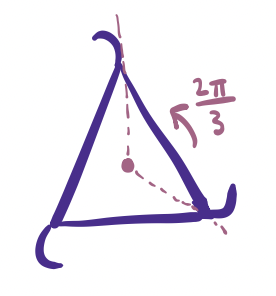
\includegraphics[width=3cm]{Lecture Files and Images/lec16-weirdtriangle.png}
\end{center}


\begin{example}[B]\label{example b}
For figure B, the translation subgroup is trivial, consisting of $0.$ Also, $\overline{G}$ is $C_3,$ since there cannot be any reflections but rotation by $2\pi/3$ or $4\pi/3$ around the center both preserve the figure.

\end{example}


\begin{center}
    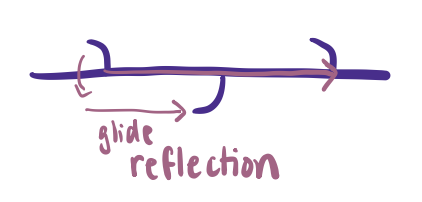
\includegraphics[width=5cm]{Lecture Files and Images/lec16-glide.png}
\end{center}

\begin{example}[C]\label{example c}
For figure C, the translation subgroup is generated by one vector, so $L = \ZZ\alpha$ where $\alpha = (1, 0)$. Also, $\overline{G}$ is $D_1,$ since there is a reflection (corresponding to a glide reflection in $G$) and no rotations possible. 
\end{example}


\begin{center}
    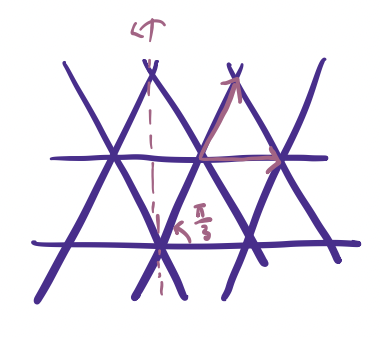
\includegraphics[width=5cm]{Lecture Files and Images/lec16-latticetriangle.png}
\end{center}
\begin{example}[D]\label{example d}
For figure D, the translation subgroup is a triangular lattice generated by two vectors at an angle of $\pi/3$ to each other.\footnote{Or two vectors at an angle of $2\pi/3$.} The point group is $\overline{G} = D_6,$ since rotation at a lattice point by any multiple of $\pi/3$ preserves the figure, as well as reflection. 

\end{example}

%write down 4:06

\subsection{Crystallographic Restriction}
Now that we have decomposed studying $G$ into studying groups we understand better, $L$, a subgroup of translations, and $\overline{G} \subseteq,$ the point group, we can actually constrain $G$ further! 

Recall that 
\begin{itemize}
    \item The translation subgroup $L \subseteq (\RR^2, +)$\footnote{The translation subgroup $L$ is sometimes written ambiguously in one of two equivalent ways; an element of $L$ can either be the translation $t_{\vec{b}} \in L$ considered as an element in $G,$ or simply the vector $\vec{b} \in L$ considered as an element in $\RR^2.$ So $L$ could be considered either as a subgroup of $G$ or of $\RR^2.$} must be one of three possibilities, which we get from studying discrete subgroups of $\RR^2$; %check if footnote makes sense LOL
    \item  $\overline{G}$ must be $C_n$ or $D_n,$ which we get from studying discrete subgroups of $O_2.$
\end{itemize}
 Now that we understand the components $L$ and $\overline{G}$ separately, we want to use this knowledge to understand $G$ better. %?? 11:17

\begin{qq}
How do $L$ and $\overline{G}$ interact with each other?
\end{qq}

\begin{example}
Consider our earlier example \ref{example d}. In this case, any element of the point group $D_6$ preserved the triangular lattice.
\end{example}

In fact, $\overline{G}$ acts on $L$ for any discrete group $G \subseteq M_2$; this is a very strong constraint on how $\overline{G}$ and $L$ interact.

\begin{theorem}\label{point group acts on l}
For the point group $\overline{G}\leq O_2$ of some discrete subgroup $G$ of $M_2,$ and the translation subgroup $L \subset \RR^2,$ the group $\overline{G}$ must map $L$ to itself. 

For any element $A \in \overline{G}$ and $b \in L,$ the image of $b$ under the action of $A$ is
\[
b \mapsto Ab \in L.
\]



%for any element of the point group $A \in \overline{G},$ and any element of the translation subgroup $b \in L,$ the element $A$ takes $b \mapsto Ab $ \mapsto Ab \in L.$
\end{theorem}

We already know that $O_2$ and thus $\overline{G}$ acts on the plane $\RR^2$ and therefore $L.$ The surprising part is that under the action of any element of $\overline{G}$, an element of $L$ is actually mapped to another element in $L$!


\begin{proof}
Since $A \in \overline{G},$ it is the image of an element of $G,$ say $t_{\vec{c}} \circ A \in G$ for some $\vec{c} \in \RR^2.$ Then, $\vec{b} \in L,$ so $t_{\vec{b}} \in G$. The key observation in this proof is that $L = \ker(\pi|_G)$ is the kernel of a homomorphism! Thus, the subgroup $L \nsub G$ is actually normal, so conjugating an element of $L$ by anything in $G$ stays in $L.$

Then for $t_{\vec{b}} \in L,$
\[
(t_{\vec{c}} \circ A) \cdot t_{\vec{b}} \cdot (t_{\vec{c}} \circ A)^{-1} \in L
\]
also. As isometries in $M_2,$ we know how to manipulate these products, and so expanding out this expression gives us 
\begin{align*}
    t_{\vec{c}} \cdot A \cdot t_{\vec{b}} \cdot A^{-1} \cdot t_{\vec{c}}^{-1} &= t_{\vec{c}} t_{A\vec{b}} \cdot A \cdot A^{-1} \cdot t_{-\vec{c}} \\
    &= t_{\vec{c}} t_{A\vec{b}} t_{-\vec{c}} \\
    &= t_{A\vec{b}} \in L.
\end{align*}

Thus, conjugating $t_{\vec{b}} \in L$ by $t_{\vec{c}} \circ A$ gives $t_{A\vec{b}} \in L.$ Using the identification of $L$ with $\RR^2,$ $A \vec{b} \in L \subset \RR^2$, and so every $A \in \overline{G}$ takes vectors $\vec{b}$ in $L$ to other vectors in $L,$ preserving the translation subgroup.
\end{proof}

\begin{question}%[Student Question]

We're studying discrete groups, which are groups with the requirement that the translations or rotations can't be arbitrarily small. Are we also requiring that they have to be groups preserving a given diagram, or can they be any discrete groups of isometries? 


%So with these discrete groups, we have a requirement that they can't be arbitrarily small but are we also saying that they can't be just any isometries they have to preserve the diagrams? 

\end{question}
\begin{ans}
Earlier on in this lecture, we saw some \textbf{examples} of discrete groups $G$ that came from the symmetry groups of certain diagrams, but what we are actually doing is simply looking at groups $G$ with the condition that the rotations and translations must be arbitarily small\footnote{These are called discrete groups}, and classifying them; mathematically, there is no requirement that they come from pictures. 

However, the way that these discrete groups actually show up and the way that we find them is by drawing these kinds of pictures; this is one of the main reasons why we care about them! In fact, for every discrete subgroup $G \subseteq M_2,$ there \emph{will be} some picture that produces the group $G$ as its symmetry group. The pictures in this lecture are mainly so that there are concrete examples to look at and think about. 

In Section \ref{examples for l and g}, each of the examples has a symmetry group $G$ consisting of the isometries of the plane sending the picture to itself.\footnote{Not each point individually is sent to itself; the picture as a whole is sent to an identical copy of itself.} For example, in Example \ref{example b}, rotation by 120 degrees preserves the "triangle," while 5 degrees does not, so $\rho_{2\pi/3} \in G,$ whereas $\rho_{\pi/36} \notin G.$ 

%what we are actually doing is taking some group $G$ and the rotations and translations can't be arbitrarily small. but they come from these pictures! IN FACT, for every $G$, there is some picture where $G$ is the symmetry group of this picture. 

\end{ans}

Theorem \ref{point group acts on l} states that the point group $\overline{G}$, which is a different group from $G,$ actually preserves $L \subseteq \RR^2,$ the translation group. 

In Example \ref{example d}, $L$ is generated by 
\[
\ZZ(1, 0)^t + \ZZ(1/2, 3/2)^t,
\]
the two sides of an equilateral triangle, and the point group is $D_6.$ Any element of $D_6$ will send an element of $L$ to a different element in $L.$

In fact, when $L$ is a lattice, preservation by some point group $\overline{G}$ is a strong constraint on the possible angles that show up in the lattice; only certain angles are allowed. Given $\overline{G},$ most lattices are not preserved by every element. Thus, the theorem constrains $\overline{G}$ and $L$ together --- not on each of them separately, but on how they interact. 

The groups that show up this way are often called crystallographic groups. \footnote{Especially when $L$ is a lattice, and there are two different directions to translate.} They are well-studied; in fact, there are only finitely many.

%question: is it the point group crystallographic? or the group G?

\begin{theorem}[Crystallographic Restriction]\footnote{The theorem name comes from the fact that it restricts the possible crystallographic groups.}
Let $L \neq \{0\}.$ Then $\overline{G} = C_n$ or $D_n$, where $n = 1, 2, 3, 4,$ or $6.$
\end{theorem}

%So before, it looked like we had lots of possibilities even before the discreteness condition, but since they have to interact with each other, it really narrows it down. Only certain choices of $L$ are allowed for a given $n.$

Although we could imagine that there are lots of possibilities for $\overline{G}$ and $L,$ the fact that $\overline{G}$ preserves $L$ constrains the possible point groups to finitely many, and there are also only certain choices of $L$ allowed for a given $n.$

%question: how many G are there total? is this true in higher dimensions?

\begin{proof}
The group $\overline{G}$ is a discrete subgroup of $O_2,$ and so it is $C_n$ or $D_n$ for some integer $n.$

Since $L$ is discrete, there is a (non-unique) shortest nonzero vector $\alpha \neq 0$. Consider a rotation $\rho = \rho_\theta \in G.$ The result of rotating $\alpha$ by $\theta$ is another vector in $L$, and since rotations are length-preserving, $\rho_{\theta} \alpha$ is also a vector of shortest length. Since both vectors are in $L,$  $\rho\alpha - \alpha$ is also in $L.$\footnote{Since $L$ is a subgroup, it is closed under addition/subtraction.} If $\theta$ is too small, $\rho\alpha - \alpha$ will have a shorter length, and there will be a contradiction. 

In particular, if $\theta < 2\pi/6,$ $\rho\alpha - \alpha$ is shorter than $\alpha$, so $\theta \geq 2\pi/6.$ Since $C_n$ and $D_n$ contain $\rho_{2\pi/n},$ it must be the case that $n \leq 6.$ 
\begin{center}
    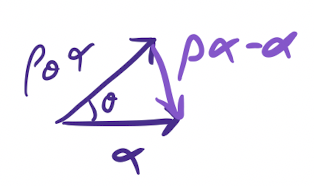
\includegraphics[width=4cm]{Lecture Files and Images/lec16-thetatriangle2.png}
\end{center}

A similar argument holds to rule out $n = 5.$ The vector $\alpha + \rho_{4\pi/5} \alpha$ will be shorter than any $\alpha$, which is also a contradiction.\footnote{This question is equivalent to the feasibility of tiling the plane with a regular pentagon, and in fact that is not possible!}%31:05

\begin{center}
    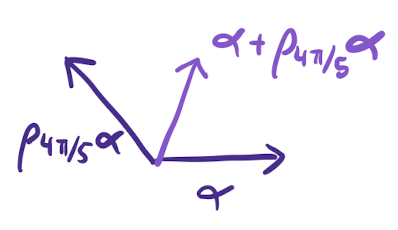
\includegraphics[width=4cm]{Lecture Files and Images/lec16-nis52.png}
\end{center}

So $n = 1, 2, 3, 4,$ or 6.  
\end{proof}
Actually, for $C_n$ or $D_n$ where $n = 1, 2, 3, 4$, or 6, it is possible to constrain the translation subgroups $L$ that can simultaneously show up.

For instance, when $L$ is a lattice,\footnote{When $L$ is a lattice, it is two-dimensional, and it is $\ZZ\vec{a} + \ZZ\vec{b}$ for generating vectors $\vec{a}$ and $\vec{b}.$ It is also possible for $L$ to be $\ZZ\vec{a}$, which is one-dimensional.} there are only 17 possible symmetry groups $G$ that can occur. When $L$ is 0, $\overline{G}$ can be $C_n$ or $D_n$ for any arbitrary $n$, but allowing nontrivial translations constrains $\overline{G}$ significantly.

\begin{question}%[Student Question]
How much does constraining $\overline{G}$ and $L$ constrain the actual symmetry group $G$ itself?
\end{question}

\begin{ans}
Finding $G$ from $\overline{G}$ and $L$ is precisely the same as figuring out the 17 plane symmetry groups,\footnote{These are called wallpaper groups, since wallpapers are 2-dimensional patterns that usually have nontrivial symmetry groups.} and is precisely the last step! We will do one example now.
\end{ans}

Let's consider a specific group $\overline{G}$ and try to figure out what the actual symmetry group $G$ can be!

\begin{example}[$C_4$]
Suppose $\overline{G} = C_4.$\footnote{Rotations by 90 degrees, but no reflections.} Then $L \subset G \xrightarrow[]{\pi|_G} C_4,$ and the index $[G: L] = 4.$\footnote{The index $[G: \ker(\pi|_G)] = [G:L]$ is equal to the size of the image under $\pi|_G$, which is $\overline{G} = C_4.$} 

Also, $\overline{\rho} = \rho_{\pi/2} \in \overline{G}$ is a generator of $\overline{G}.$ Where $\alpha$ is some shortest-length vector in $L,$ it's possible to show\footnote{There is a more involved argument there, but it is not super relevant here.} that $\rho\alpha$ and $\alpha$ do generate $L.$ Thus,
\[
L = \ZZ\alpha + \ZZ(\rho\alpha),
\]
a square lattice.

Also, there exists some rotation $\rho \in G$ giving $\pi(\rho) = \overline{\rho.}$ Then $\rho$ is in fact a rotation by $\pi/2$ around some other point, which we will call the origin.\footnote{In the discussion of the four kinds of isometries in $M_2,$ the elements which were mapped to rotations were in fact rotations around some point.} The group $G$ contains $L$, of index 4, as well as some rotation by $\pi/2,$ $\rho.$\footnote{The rotation $\rho$ is $\overline{\rho},$ lifted to be in $G,$ and it is an element of $G$ not in $L$ which generates the quotient, $C_4.$}

\begin{center}
    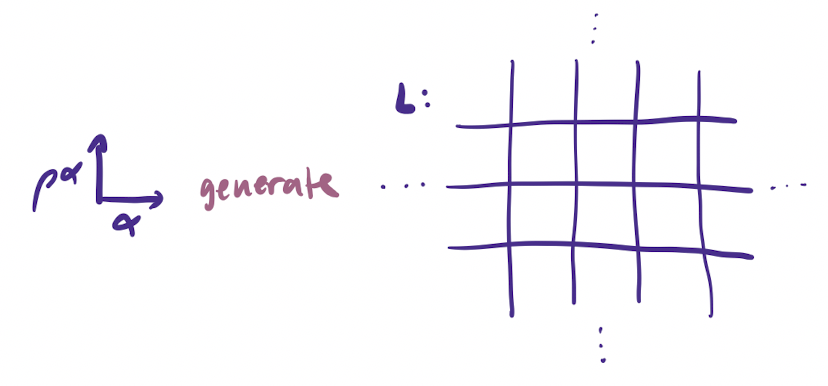
\includegraphics[width=5cm]{Lecture Files and Images/lec16-lattis.png}
\end{center}

Thus, $G$ is "generated" by $L$ and $\rho,$ and must consist of everything of the form 
\[
G = \{t_v \circ \rho^i: \vec{v} \in L, i = 0, 1, 2, 3\}.
\]

Also, $\rho t_v = t_{\rho v} \circ \rho,$ so the group multiplication can be written down, and $G$ is completely determined by knowing that $\overline{G}$ was $C_4$; this is 1 out of the 17 wallpaper groups!
\end{example}

\begin{question}
Can you explain where $\rho$ came from? Why is it a rotation? 
\end{question}

\begin{ans}
By definition, $\overline{G}$ is the image of $G$ under $\pi: M_2 \rightarrow O_2$ taking $t_b \circ A \mapsto A.$ Then there are four possibilities for elements in $M_2$: translation, rotations, reflections, and glide reflections. The first two are orientation-preserving, and the last two are orientation-reversing. Reflections and glide reflections map to reflections in $O_2$\footnote{Reflections across lines through the origin} under $\pi,$ translations will map to the identity, and rotations will map to rotations (around the origin). So $\rho$ has an image of $\overline{\rho},$ which is a rotation, and thus $\rho$ is a rotation around some point.
\end{ans}

If $\overline{\rho},$ the element in $\overline{G},$ were a reflection instead of a rotation, the preimage in $G$ could have been either a reflection or a glide reflection, so when the point group $\overline{G} = D_n$, one of the dihedral groups, instead of $C_n,$ the analysis is more subtle. In fact, there might not be any reflections in $G$ at all. (In Example \ref{example c}, there were no reflections, only glide reflections.) 

%A reflection $\overline{r} \in \overline{G}$ is $\pi(r)$ for $r \in G,$ where $r$ could be either a reflection or a glide reflection.

\begin{example}

If $\overline{r} = \pi(r)$ where $r$, then $\overline{r} = \pi(t_b \circ r_\ell),$ where $b$ is some zero\footnote{reflection} or nonzero\footnote{glide reflection} vector parallel to the line $\ell$. Does this mean there are uncountably many possibilities for $b$ and therefore $r?$ In fact, $b$ is constrained a bit more: $t_b r_\ell t_b r_\ell = t_{2b}$, so $2b \in L$. Thus, there are two possible situations: 
\begin{itemize}
    \item The vector is in the lattice: $b \in L$;
    \item The vector $b$ is halfway between two lattice points, as in Example \ref{example a}.
\end{itemize}
\end{example}

From these two examples, we see that given some $\overline{G}$, of which there are finitely many, and working through the information that is present, there aren't too many possibilities for $G$, and in fact there are finitely many --- 17 in total. 

\newpage

\lhead{Lecture 17: Group Actions}
\setcounter{section}{16}
%MIT OpenCourseWare: https://ocw.mit.edu
%RES.18-011 Algebra I Student Notes, Fall 2021
%License: Creative Commons BY-NC-SA 
%For information about citing these materials or our Terms of Use, visit: https://ocw.mit.edu/terms.

\section{Group Actions}

Today, we will discuss group operations or actions\footnote{They are different terms for the same idea. Artin uses group operations, while Professor Maulik prefers to call them group actions.} on a set.
\begin{qq}
How can a group be seen as a group of transformations?%\footnote{Like matrices, our motivating example all the way back from the first lecture!}
\end{qq}

\subsection{Review}
Last time, we finished talking about (discrete) subgroups of isometries of the plane. Finite subgroups of $M_2$ are isomorphic to $C_n$ or $D_n,$ and there are only finitely many isomorphism classes of infinite discrete subgroups of $M_2$.\footnote{In fact, with \emph{any} metric space, which is a set with some distance on it (as discussed in 18.100, for example), it's possible to consider isometries, distance-preserving transformations, in the same way as we considered the plane $\RR^2.$ Depending on the metric space, the groups can look very different! One example of this is the hyperbolic plane, which is the upper half-plane of $\RR^2$ with a non-Euclidean metric, or distance, on it, and the discrete subgroups of isometries on it. There are infinitely many discrete subgroups of isometries on it, even though it is 2-dimensional, just like $\RR^2.$ The question of why it is so different from the $\RR^2$ case is really a geometry question, rather than an algebra question.} 

It is also possible to go up a dimension and classify discrete subgroups of isometries of $\RR^3$, although it is more complicated; there are 200 or so. 



\subsection{Motivating Examples}
The idea of a group action will generalize and make more abstract an idea that has been present throughout the class so far. Let's start with the following motivating example. 
\begin{example}[$GL_n$]
Given $g \in GL_n(\RR)$ and a column vector $v \in \RR^n,$ the matrix $g$ can be seen as a transformation on $\RR^n,$ taking $v \mapsto g(v) \in \RR^n.$ 

The data of $GL_n(\RR)$ acting on $\RR^n$ can be packaged together by a map 
\begin{align*}
    GL_n(\RR) \by \RR^n &\rto \RR^n \\
    (g, \vvv) &\mto g(\vvv).
\end{align*}
\end{example}

The same principle applies to $S_n,$ the group of permutations on $\{1, \cdots, n\}$.
\begin{example}[$S_n$]
The symmetric group $S_n$ can also be viewed as acting on a set. More or less by definition, given a number between 1 and n, and a permutation, it's possible to spit out the result of permutation acting on that number. So $S_n$ permutes the set $[n] = \{1, \cdots, n\}.$
This gives us another mapping encoding this information:
\begin{align*}
    S_n \by \{1, \cdots, n\} &\rto \{1, \cdots, n\} \\
    (\sigma, i) &\mto \sigma(i).
\end{align*} 
\end{example}

Our last example is one we have been considering for the past few lectures.
\begin{example}
The set $M_2$, isometries of 2-space, acts on $\RR^2:$ given some vector in the plane and some isometry, the isometry will return some other vector in the plane. This information is again encoded by a mapping
\begin{align*}
    M_2(\RR) \by \RR^2 &\rto \RR^2 \\
    (f, \vec{x}) &\mto f(\vec{x}). 
\end{align*}
\end{example}

\subsection{What is a group action?}
These are all examples of group operations on a set, and they motivate the following definition of a group operation in general.
\begin{definition}
Given a group $G$ and a set $S,$ a \textbf{group action}\footnote{or group operation} on a set $S$ is a mapping 
\begin{align*}
    G \by S &\rto S \\
    (g, s) &\mto gs.
\end{align*}
It must satisfy the following axioms:
\begin{itemize}
    \item The identity maps every element of the set back to itself: $es = s$ for all $s \in S.$\footnote{This corresponds to the identity multiplication rule.}
    \item The mapping must respect the group multiplication: $(gh)s = g(hs)$ for $s \in S$ and $g, h \in G.$\footnote{This corresponds to the associativity rule.}
\end{itemize}
\end{definition}

Essentially, given an element $g \in G$ and $s \in S,$ the mapping returns another element of $S$ depending on $g,$ and the mapping must respect the group structure on $G.$ All of the groups that we have seen so far show up as symmetries of some set, maybe preserving some extra structure, so all the groups that we usually think about already come with an action on some set $S.$ Furthermore, a group $G$ can act on many different sets at the same time in different ways, which gives insight into the group itself.

Let's look at a couple of examples.
\begin{example}[$S_4$]
The symmetric group $S_4,$ permutations on 4 elements, acts on $S = \{1, 2, 3, 4\}$. It can \emph{also} act on a different set, $T = \{\text{unordered pairs in } S \} = \{(12),(13), (14), (23), (24), (34)\}.$ The set $T$ has 6 elements, and $S_4$ acts on $T$ as well as acting on $S.$ Given a permutation $\sigma \in S_4,$ and an unordered pair $\{i, j\},$ it acts by taking
\[
\sigma(\{i, j\}) = \{\sigma(i), \sigma(j)\}
\]
for a permutation $\sigma \in S_4.$ 
\end{example}

So the group action on $S$ leads to a different group action on a different set, $T.$ The existence of a group action on a given set actually yields a lot of information about the group $G,$ as will be explored in the next few lectures. Let's see a different example.

\begin{example}[$D_2$]\label{grp action d2}
Let $G = D_2,$ which contains rotation by $\pi$ as well as reflection across the $x$-axis (and then reflection across the $y$-axis.) As a subgroup of $O_2,$\footnote{$2 \by 2$ orthogonal matrices}, $D_2$ will act on all of $\RR^2.$ It also acts on the set $S$ consisting of the vertices of a square and a diamond, as well as the center. 

\begin{center}
    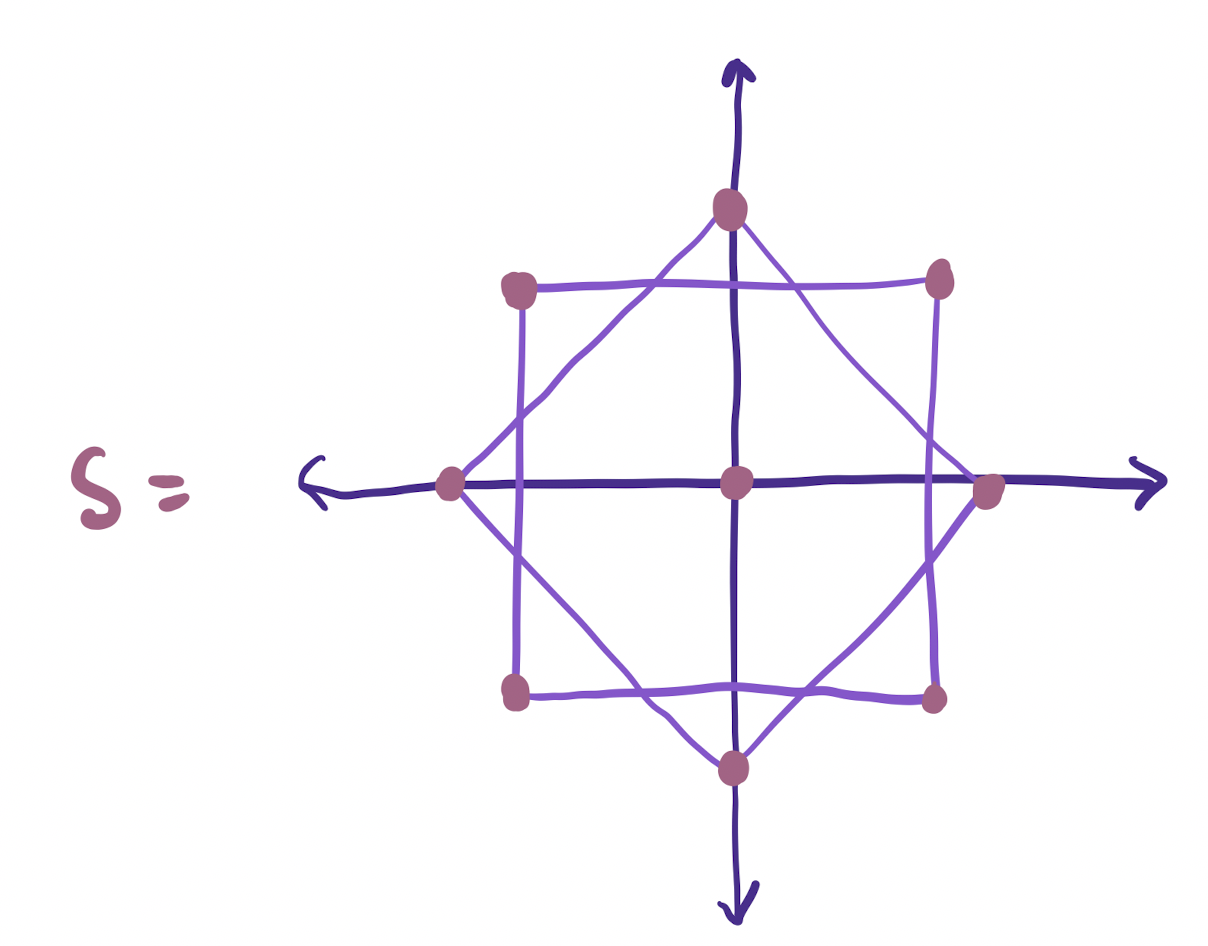
\includegraphics[width=5cm]{Lecture Files and Images/lec17-S.png}
\end{center}
\end{example}

A group $G$ can also act on itself viewed as a set.
\begin{example}
Given a group $G,$ there is a mapping
\begin{align*}
    G \by G &\rto G \\
    (g, g') &\mto gg',
\end{align*}
and this is a valid group action. 
\end{example}

When $G$ acts on itself, the first $G$ in $G \by G$ is seen as a group, while the second $G$ is seen as a set, since the axioms of a group action don't care about the group operation on the second instance of $G$.

Let's see one last example. 
\begin{example}
Taking a vector space $V$ over a field $F,$ the group $F^{\by}$, the nonzero elements of the field, which is a group with respect to multiplication, acts on $V$ by scaling:
\begin{align*}
    F^{\by} \by V &\rto V \\
    (a, \vec{v}) &\mto a\vec{v}.
\end{align*}
\end{example}

Scaling by nonzero scalars defines a group operation! It satisfies each of the axioms. 

\begin{question}
What type of element is $g(s)?$
\end{question}
\begin{ans}
It depends on what $S$ is! It is the type of element that is in $S.$ Two group actions of $G$ on $S$ and $S'$ might not have anything to do with each other, other than the fact that they both involve $G;$ $G$ can act on wildly different types of sets, and show up in different contexts.
\end{ans}

Say we fix an element $g \in G,$ we can define the group action of $g$ on $S$, a mapping $\tau_g: S \rto S$ sending $s \mto g(s).$\footnote{This notation is not standard and may not correspond with the textbook.} We can show that $\tau_g$ is a bijection from $S$ to itself because it has an inverse map, $\tau_{g^{-1}},$ coming from the fact that $g$ is invertible. Because $\tau_g$ is a bijection, it actually \emph{permutes} the elements of $S,$ and so it is a permutation of $S.$ Thus, each element of $G$ can be mapped to a permutation by a map
\[
\tau: G \rto \text{Perm}(S),
\]
which takes $g \mto \tau_g \in \text{Perm}(S).$ From the group action axioms, $\tau$ is a group homomorphism. In Example \ref{grp action d2}, $D_2$ is acting on a set with $|S| = 9,$ so there exists a homomorphism from $D_2 \rto \text{Perm}(S) = S_9.$

Note that $\tau$ does not have to be injective; there may be some action $g \in G$ such that $g \neq e$ but $G$ fixes each $s \in S,$ which would make $\tau(g)$ the identity permutation.

\subsection{The Counting Formula}

\begin{definition}
Given $s \in S,$ the \textbf{orbit} of $s$ is 
\[
O_s = Gs \coloneqq \{gs : g \in G\} \subseteq S.
\]
\end{definition}

For instance, in Example \ref{grp action d2}, there are several orbits of different sizes. The top and bottom vertices of the diamond are in the same orbit (size 2), the left and right vertices of the diamond are in the same orbit (size 2), all the vertices of the square are in the same orbit (size 4), and the origin is in an orbit by itself (size 1), just by applying each of the group elements to an element of the set.  

%** 29:40 student question

\begin{definition}
The group $G$ acts \textbf{transitively} on $S$ if $S = O_s$ for some $s \in S.$ 
\end{definition}

For example, $S_n$ acts transitively on $\{1, \cdots, n\},$ since given an element $i \in \{1, \cdots, n\},$ there is some permutation mapping it to any other element $i'.$

\begin{question}
Does this have to be true for all $s \in S,$ or just one?
\end{question}
\begin{ans}
If it is true for one $s \in S,$ it is true for all $s \in S.$ Try checking it!
\end{ans}


So a transitive group action is one where there is only one orbit consisting of the entire set $S;$ in particular, any element of $s$ can be carried to any other element when acted on by some $g \in G.$

\begin{definition}
The \textbf{stabilizer} of $s$ is 
\[
G_s = \text{Stab}_G(s) \coloneqq \{g \in G: gs = s\},
\]
and it is a subgroup of $G.$
\end{definition}

For Example \ref{grp action d2}, the top and bottom vertices of the diamond are stabilized by the reflection across the $y$-axis, whereas the stabilizer group of a vertex of the square is just the identity element.

\begin{center}
    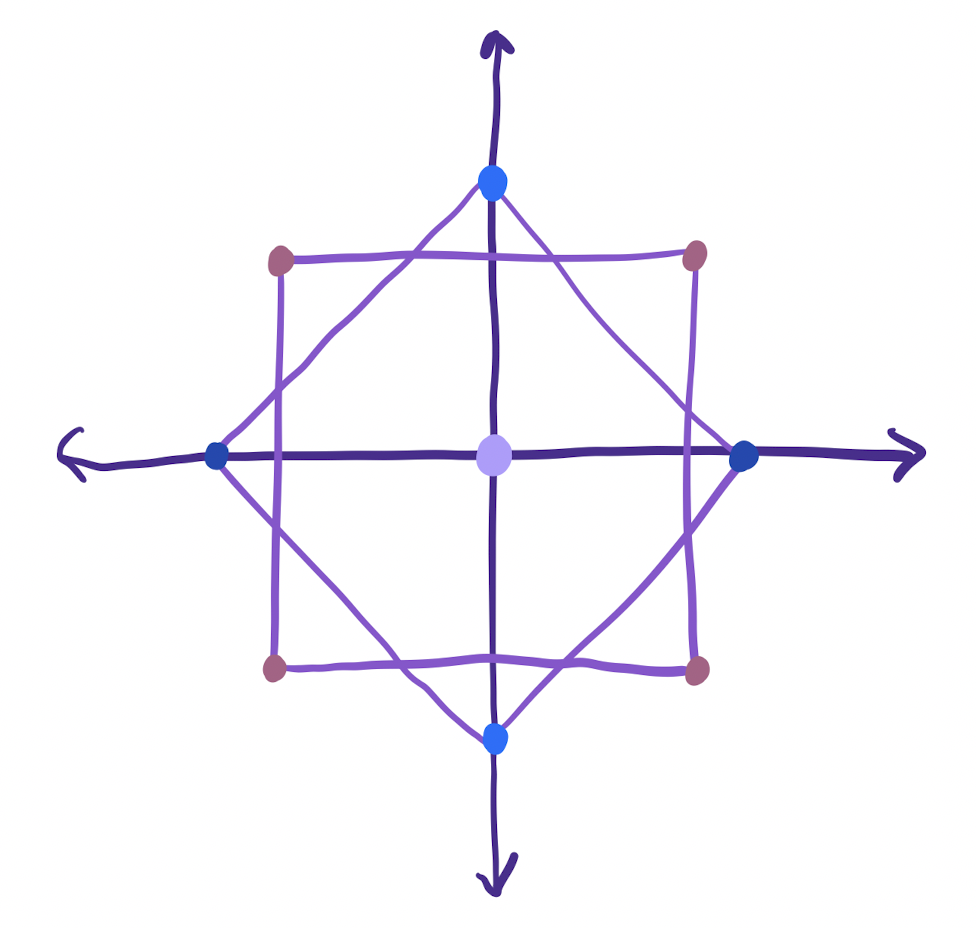
\includegraphics[width=5cm]{Lecture Files and Images/lec17-orbitsofS.png}
\end{center}

\begin{proposition}
The orbits of $G$ form a \emph{partition} of $S.$\footnote{The set can be cut into non-overlapping pieces by the orbits.} In particular, $S$ is the disjoint union of the orbits: $S = \amalg O_i$ where $O_i \cap O_j = \varnothing.$ 
\end{proposition}
\begin{proof}
The orbits clearly cover $S$, since every element $s \in S$ is also an element of $O_s,$ its own orbit. Also, they are disjoint. If $O_s \cap O_{s'} \neq \varnothing,$ then there is some element in their intersection $t = gs = g's'$. Then $s = (g^{-1}g')s',$ which is in $O_{s'}$. So every element of $O_s$ is in $O_{s'},$ and by the same logic $O_{s'} \subseteq O_s.$ Then $O_s = O_{s'}$. So if two orbits have nonempty intersection, they are in fact the same orbit.
\end{proof}

For a finite set, the size of $S$ can be obtained from the sizes of the orbits. 

\begin{corollary}
If $S$ is a finite set, and $O_1, \cdots, O_k$ are the orbits, then 
\[
|S| = \sum_{i = 1}^k |O_i|,
\]
since each of the orbits cover $S$ exactly.
\end{corollary}

In Example \ref{grp action d2}, this gives $9 = 4 + 2 + 2 + 1.$

\begin{qq}
What does each orbit look like?
\end{qq}

For this, we use the notion of a \emph{stabilizer} of an element.

\begin{proposition}
Fix some $s \in S$ and let $H \coloneqq \text{Stab}(s).$ Then there exists a bijection $\varepsilon$ from the quotient group $G/H$ to the orbit of $s,$ $O_s.$ It takes 
\begin{align*}
    G/H &\xrightarrow[]{\varepsilon} O_s \\
    gH &\mapsto gS.
\end{align*}
\end{proposition}

\begin{center}
    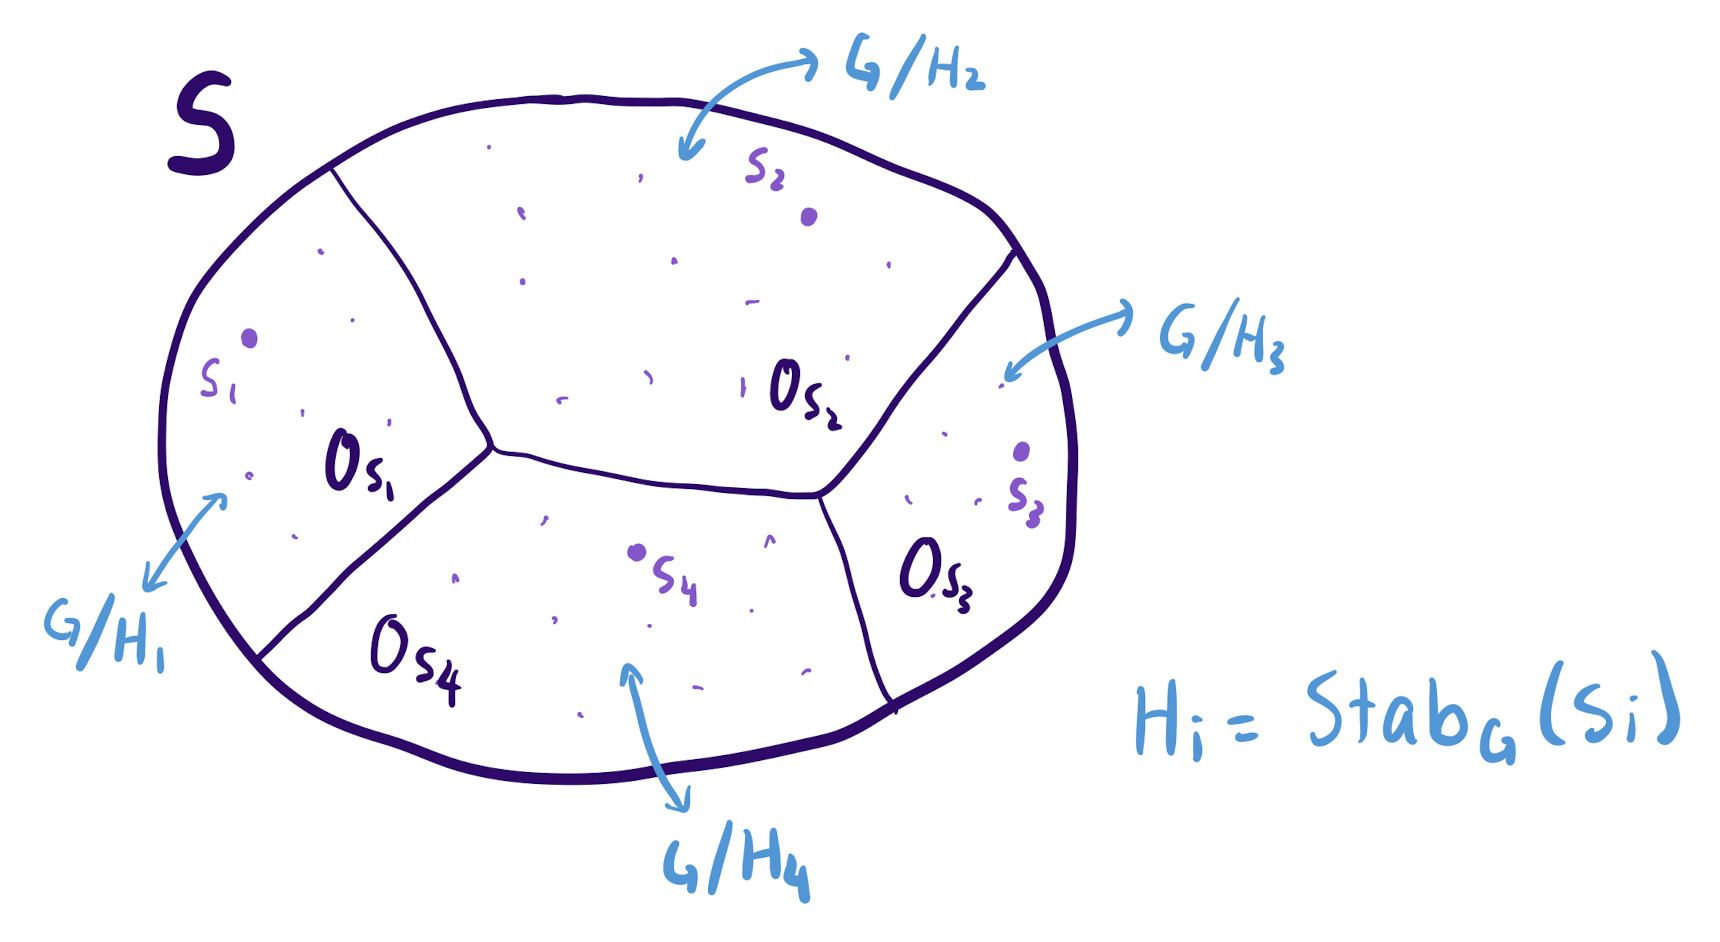
\includegraphics[width=12cm]{Lecture Files and Images/lec17-drawing.png}
\end{center}


\begin{proof}
Consider $g$ and $\gamma$ in $G.$ Then their cosets map to the same element if $gs = \gamma s,$ which is equivalent to saying that $g^{-1}\gamma s = s$. Since $H$ is the stabilizer of $S,$ this means that $g^{-1}\gamma \in H;$ equivalently, $\gamma \in gH.$ Since each of these conditions were equivalent conditions, $gs = \gamma s$ if and only if $\gamma \in gH,$ and thus $\varepsilon$ must be bijective: two elements in $G/H$ map to the same element in $O_s$ if and only if they are the same element.
\end{proof}

\begin{corollary}[Counting Formula for Orbits]
As a result, the number of cosets of $H$, which is the order $|G/H|$, is equal to the size of the orbit of $s,$ since there is a bijective correspondence between them. So 
\[
|O_s| = [G : \text{Stab}(s)].
\]
\end{corollary}

In particular, the size of the orbit of any element $|O_s|$ divides $|G|$ when $G$ is a finite group. We have 
\[
|O_s|\cdot|\text{Stab}(s)| = |G|.
\]

These theorems are similar to the Counting Formula and Lagrange's Theorem from Chapter 2. In particular, let $\mathcal{C}$ be the set of left cosets of a given subgroup $H.$ Then $G$ acts on $\mathcal{C}$; an element $g \in G$ takes $C \mto gC.$ Every coset can be mapped to any other coset by some element of $G.$ For example, $g_1H$ is mapped to $g_2H$ by $g_2g_1^{-1}\in G.$ So there is only one orbit, the entire set $\mathcal{C}$. The stabilizer of the identity coset, which is $eH = H,$ is $\text{Stab}(eH) = H,$ because some element $g \in G$ carries $h \in H$ to $h' \in H$ if and only if $gh = h',$ which implies that $g = h'h^{-1} \in H.$ Thus, the Orbit-Stabilizer Theorem states that 
\[
|G| = |H|[G:H],
\]
since $|H|$ is the stabilizer of the identity in $G/H$ and $[G:H]$ is the size of the identity orbit.


\begin{example}
Consider the subgroup $G \leq SO_3$ consisting of rotational symmetries of a cube centered at the origin. 


\begin{center}
    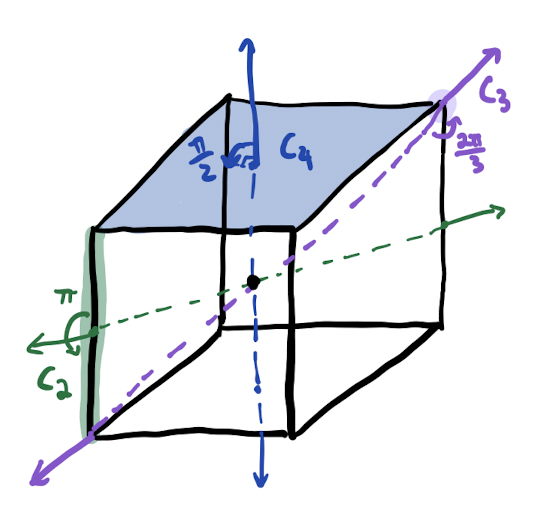
\includegraphics[width=7cm]{Lecture Files and Images/lec17-cube.png}
\end{center}


\begin{itemize}
    \item Let $S$ be the set of faces of the cube; it has order 6 since there are 6 faces. For every face of the cube, there is some element in $G$ mapping it to any other face in the cube ($G$ acts transitively on the faces), so the orbit of a given face is the set of all the other faces, which is $S.$ The stabilizer $\text{Stab}_G(\text{face}) = C_4,$ since a given face, which is a square, is preserved by rotation by $\pi/2$ around the axis through the center of the face. Then 
    \[
    |G| = |S| \cdot |\text{Stab}_G(\text{face})| = 6 \cdot 4 = 24.
    \]
    
    \item Similarly, any vertex can be mapped to any other vertex by some element of $G.$ The stabilizer $\text{Stab}_G(\text{vertex}) = C_3,$ since a vertex is preserved under rotation by $2\pi/3$ around the axis from the vertex to the opposite vertex. Again, 
    \[
    |G| = |\{\text{vertices}\}|\cdot|\text{Stab}_G(\text{vertex})| = 8 \cdot 3 = 24.
    \]
    
    \item Again, $G$ acts transitively on the set of edges. The stabilizer of an edge is $\text{Stab}_G(\text{edge}) = C_2$. Then 
    \[
    |G| =  |\{\text{edges}\}|\cdot|\text{Stab}_G(\text{edge})| = 12 \cdot 2 = 24.
    \]
\end{itemize}

\end{example}

\newpage

\lhead{Lecture 18: Geometric Application of Stabilizer}
\setcounter{section}{17}
%MIT OpenCourseWare: https://ocw.mit.edu
%RES.18-011 Algebra I Student Notes, Fall 2021
%License: Creative Commons BY-NC-SA 
%For information about citing these materials or our Terms of Use, visit: https://ocw.mit.edu/terms.

% \section{Finite subgroups of \texorpdfstring{$SO_3$}{SO3}}

\section{Stabilizer}

\subsection{Review}
A group action is when a group $G$ acts on a set $S$ by 
\[
G \by S \rto S
\]
and sends
\[
(g, s) \mto gs.
\]

The orbit of an element in $s$ is all the elements it gets mapped to,
\[
O_s = \{gs \in S : g \in G\},
\]
and the stabilizer is 
\[
\stab_G(s) \coloneqq \{g \in G: gs = s\} \leq G,
\]

\subsection{Counting Formula}
\begin{figure}[h]
    \centering
    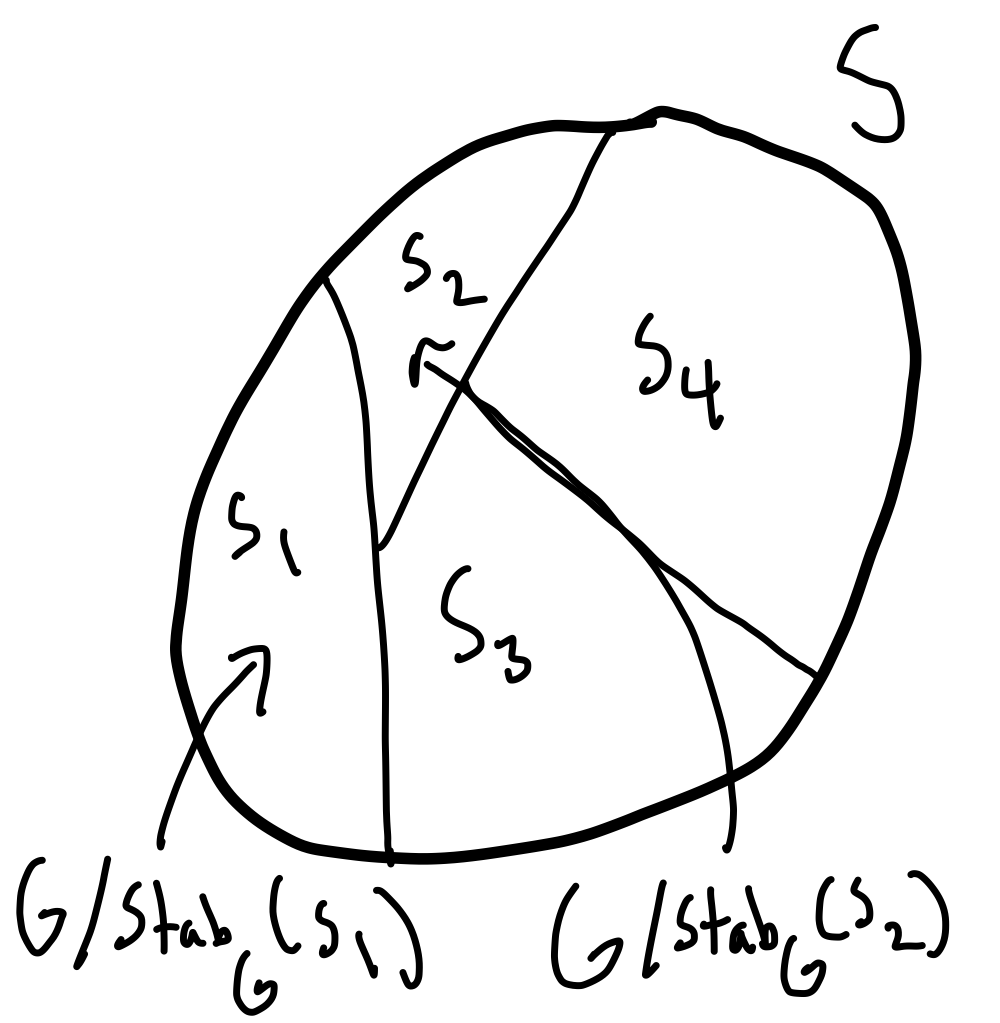
\includegraphics[width=6cm]{Lecture Files and Images/lec18-orbits.png}
    \caption{The partition of $S$ into orbits and theeir corresponding bijections with $G/\stab(s_i)$}
\end{figure}

One of the facts we learned about orbits is that they partition $S$. 
We further learned that there is a bijection between the left cosets of the stabilizer with the orbit.
We were then able to write the size of $S$ as 
\[
|S| = \sum |O_{s_i}| = \sum [G: \stab(s_i)].
\]


\subsection{Stabilizers of Products}
Given a group $G$ acting on a set $S$ and an element $s\in S$, we know that $|O_s| = [G:\stab(s)].$
This also means that we expect that if we take the stabilizer of two elements in the same orbit, then they should be the same size. Specifically, we are asking what can we say about the stabilizer of a product. If $s' = as$ for $a \in G,$ if $g \in \stab(s),$ then $gs = s.$ 
Then 
\[
aga^{-1}(s') = aga^{-1}(as) = ag(s) = as = s'.
\]
In other words, if $g$ stabilizes $s$, then $aga^{-1}$ stabilizes $s'$. 
So the upshot is that 
\[
\stab_G(s') = a\stab_G(s)a^{-1}.
\]
If $\stab_G(s')$ was normal, then the two stabilizers would be the same, but this doesn't have to be the case. 
We've provided a nice bijection to see that the sizes of the two stabilizers must be the same size.
\subsection{Statement}
Today, we will look at a consequence of these counting formulae.
Recall that we were able to study and classify finite and discrete subgroups of isometries in the plane. 
The special orthogonal group $SO_3$ is the group of rotations $\rho_{(u, \theta)}$ in $\RR^3$ fixing $\vv{0}$. What are the finite subgroups $G \leq SO_3$?

In fact, there are not so many! Let's start with the theorem.
\begin{theorem}
If $G \leq SO_3$, then 
\begin{itemize}
    \item $G \cong C_n = \langle \rho_{u, 2\pi/n}\rangle$, or
    \item $G \cong D_n = \langle \rho_{u, 2\pi/ n}\rangle$, or 
    \item $G$ is the group of rotational symmetries of a regular polyhedron.
\end{itemize}
\begin{figure}[H]
    \centering
    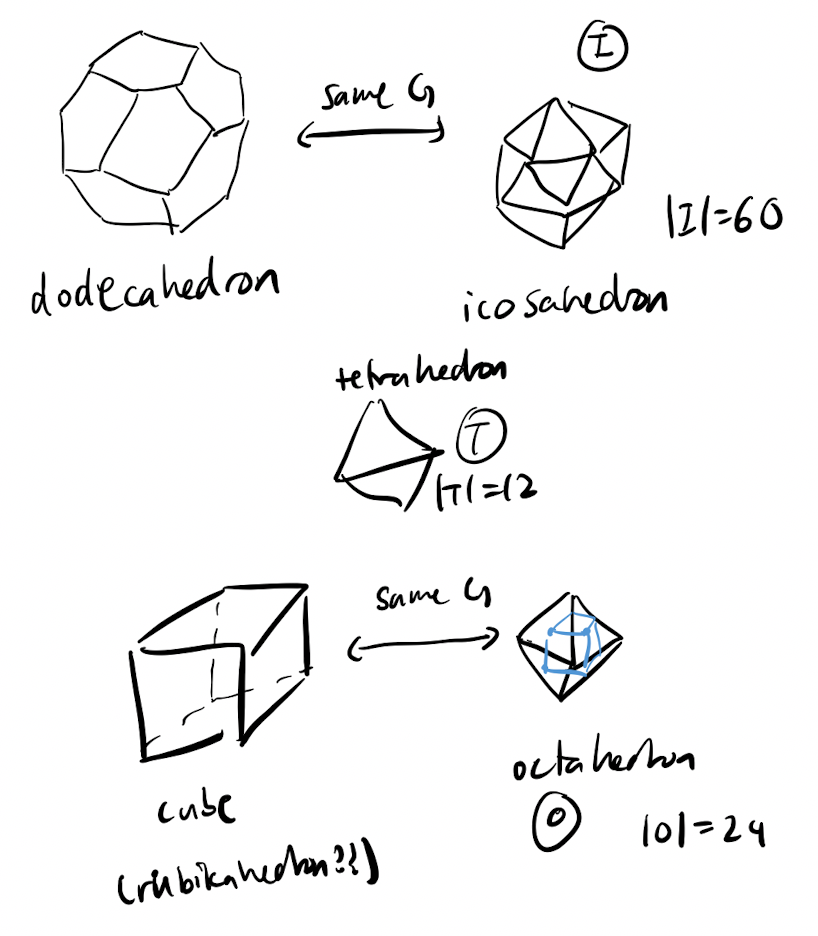
\includegraphics[width=10cm]{Lecture Files and Images/lec18-hedra.png}
    \caption{The regular polyhedra}
\end{figure}

\end{theorem}
Although there are 5 regular polyhedra, there are only 3 distinct subgroups of symmetries. 
The dodecahedron and icosahedron have the same symmetries, which we denote as $I$.
The cube and octahedron have the same symmetries as well, which we denote by $O$.
Finally, the tetrahedron is partnered with itself and we denote its symmetries with $T$.

As an example to see why some of the symmetries are the same, consider the symmetries of the octahedron. 
We can draw a point on the center of every face in the octahedron. 
Connecting these points lead to a cube, and thus any rotational symmetry of the cube will give a symmetry of the octahedron, and vice versa. 
A similar argument can be applied to the dodecahedron and icosahedron.
Trying the argument for a tetrahedron just maps to the tetrahedron itself.

On Wednesday, we worked out that the group of symmetries of a cube has size 24. Similarly, the tetrahedron has $|T| = 12,$ and $|I| = 60.$

%9:08
We will prove this by studying orbits! An non-identity element $g \neq I \in G$\footnote{We use $I$ for the identity here} is a rotation and thus fixes two unit vectors, which are exactly the positive and negative unit vectors on the rotation axis of $g$. These are called the \emph{poles} of $g.$ Let 
\[
\mathcal{P} = \bigcup_{g \neq I} \{\text{poles of }g\}.
\]

\begin{lemma}
If $p \in \mathcal{P}$ and some $g \in G,$ then $gp \in \mathcal{P}$ also. As a result, we learn that $G$ acts on $\mathcal{P}$. 
\end{lemma}

\begin{proof}
For $p \in \mathcal{P}$, then there exists $h \neq I \in G$ such that $hp = p.$ If $p' = g(p).$ Then $ghg^{-1}(p') = p'$ by earlier reasoning. Then $ghg^{-1} \in G$, and $ghg^{-1}\neq I$ since $h \neq I.$ thus $p' \in \mathcal{P}$ also.
\end{proof}

\begin{example}
\label{CyclicPoles}
Let $G = C_n$. Then $\mathcal{P} = \{p, -p\}$ since every rotation will have the same poles.
\end{example}

\begin{example}
\label{PolyhedraPoles}
Let $G = O.$\footnote{The group of symmetries of an octahedron.} Then $\mathcal{P} = \{\text{pole for each vertex, edge, or face}\}.$ %14:53
\end{example}

Now, what can we say about stabilizers of these subgroups. let $|G| = N.$ Let's decompose $\mathcal{P}$ into orbits. Then $\mathcal{P} = \mathcal{O}_1 \cup \mathcal{O}_2 \cup \cdots \cup \mathcal{O}_k$. Then $|\mathcal{O}_i| = n_i,$ and $\mathcal{O}_i = \mathcal{O}_{p_i}$ for some pole $p_i$. Then by our relations about the number of index of the stabilizer
\[
|\stab(p_i)| = r_i = \frac{N}{n_i}.
\]
Note that the stabilizer group will be a cyclic group.
Geometrically, it will just contain the rotations around the axis $p_i$.

\subsection{Finding the subgroups}

Let's write down an auxiliary set. It is the set of poles \emph{and} group elements paired together. Let 
\[
S \coloneqq \{(g, p), g \neq I, p \text{ is a pole for }g\}.
\]

Then we can count the order of $S$ in two different ways. 

The order of $S$ is
\[
|S| = \sum_{\substack{g \in G\\ g \neq I}} 2 = 2(N-1),
\]
since there are two poles for every non-identity element of $G.$

Additionally, since we have $k$ orbits,
\[
|S| = \sum_{p \in \mathcal{P}} |\stab(p)|  - 1 = \sum_{i = 1}^k n_i(r_i - 1) = \sum_{i=1}^k \frac{N}{r_i}(r_i - 1).
\]

Every pole in the same orbit has the same stabilizer size, so we can group them together.
Now, we have that 
\[
\sum_{i = 1}^k \frac{N}{r_i}(r_i-1) = 2(N-1). 
\]

Dividing by $N,$
\[
\left(1 - \frac{1}{r_1}\right) + \left(1 - \frac{1}{r_2}\right) + \cdots + \left(1 - \frac{1}{r_k}\right) = 2 - \frac{2}{N}.
\]

Each of these quantities $1 - \frac{1}{r_1}$ is between $1/2$ and $1,$ since $r_1$ must be at least two (by the definition of a pole.) %??
So $1 - \frac{1}{r_1} \in \left[\frac{1}{2}, 1\right).$

In addition $2 - \frac{2}{N} \in [1, 2).$ So $k = 2$ or 3, since this is the only way the counting formula works out from our bounds. 
In fact, this works out for examples \ref{CyclicPoles} and \ref{PolyhedraPoles}. 
For $G=C_n$, we have two orbits, and for $G=O$ we have three orbits, even though it is much more complicated.

For $k = 2,$ when there are two orbits, 
\[
1 - \frac{1}{r_1} + 1 - \frac{1}{r_2} = 2 - \frac{2}{N},
\]
and so
\[
\frac{1}{r_1} + \frac{1}{r_2} = \frac{2}{N}.
\]
But since $r_1, r_2 \leq N,$ 
\[
\frac{2}{N} \leq \frac{1}{r_1} + \frac{1}{r_2} = \frac{2}{N}.
\]

We have $r_1 = r_2 = N,$ and $n_1 = n_2 = 1.$ Each of the poles is fixed by the \emph{entire} group. Then $G$ is a finite subgroup of $SO_2,$ and thus $G = C_N,$ a cyclic subgroup.

For the three-orbit case, the numerics of the problem is also extremely constraining. When $k = 3,$ the equation is 
\[
1 - \frac{1}{r_1} + 1 - \frac{1}{r_2} + 1 - \frac{1}{r_3} = 2 - \frac{2}{N},
\]
and equivalently 
\[
\frac{1}{r_1} + \frac{1}{r_2} + \frac{1}{r_3} = 1 + \frac{2}{N}.
\]
Without loss of generality, let $r_1 \leq r_2 \leq r_3.$ It is necessary for $r_1 = 2,$ or else the LHS\footnote{left hand side} would be $\leq 1.$ If $r_2\geq 4,$ then $r_3 \geq 4$ as well, and again the LHS would be $\leq 1.$ So $r_2 = 2$ or $3.$ Finally, if $r_2 = 3,$ then $r_3$ cannot be $\geq 6,$ again from the numerics of the problem. So $r_3 = 3, 4,$ or 5. 

In total, the cases are 
\begin{itemize}
    \item \textbf{Case 1.} $(2, 2, r):$ $r = N/2$. In this case, we still have an infinite family. 
    \item \textbf{Case 2.} $(2, 3, 3)$. We can solve for $N$ to get $N = 12.$ This corresponds to the tetrahedral group $T.$
    \item \textbf{Case 3:} $(2, 3, 4)$. $N = 24$. This corresponds to the octahedral group $O.$
    \item \textbf{Case 4:} $(2, 3, 5)$. $N = 60.$ This corresponds to the icosahedral group $I.$
\end{itemize}

We can really \emph{strongly} limit the possibilities of a group $G$. We got this by counting a set $S$ in two different ways, and playing around with the numbers and fractions. %30:21

We aren't done; we still have to show that these cases \emph{actually} correspond to the groups. In each of these cases, we have three orbits, and those correspond to edges, faces, and vertices of these regular polyhedra. The pole for any vertex can be rotated to the pole for any other vertex. We'll do the argument for the octahedral group and it will be similar for the remaining polyhedra.

\subsection{The Octahedral Group}
\begin{example}[Octahedral group]
Let's take (2, 3, 4) and argue that this group \emph{must} be symmetries of a cube or an octahedron. For $4,$ $n_3 = 6.$ So the stabilizer has size 4 and the orbit has size 6. Let's try to figure out what the orbit looks like. It contains six vectors inside $\RR^3,$ so we can simply see the possible configurations. 

Drawing the first vector is easy; we just pick wherever we want for $p.$ Then $-p$ has to be in the same orbit as well because $\stab_G(-p)$ has the same order as $\stab_G(p),$ but we only have one orbit with stabilizer size 4. What does the stabilizer group look like? Geometrically, it's rotations around $p$ and must have size 4, so we have $\stab_g(p) = C_4.$ 
\begin{center}
    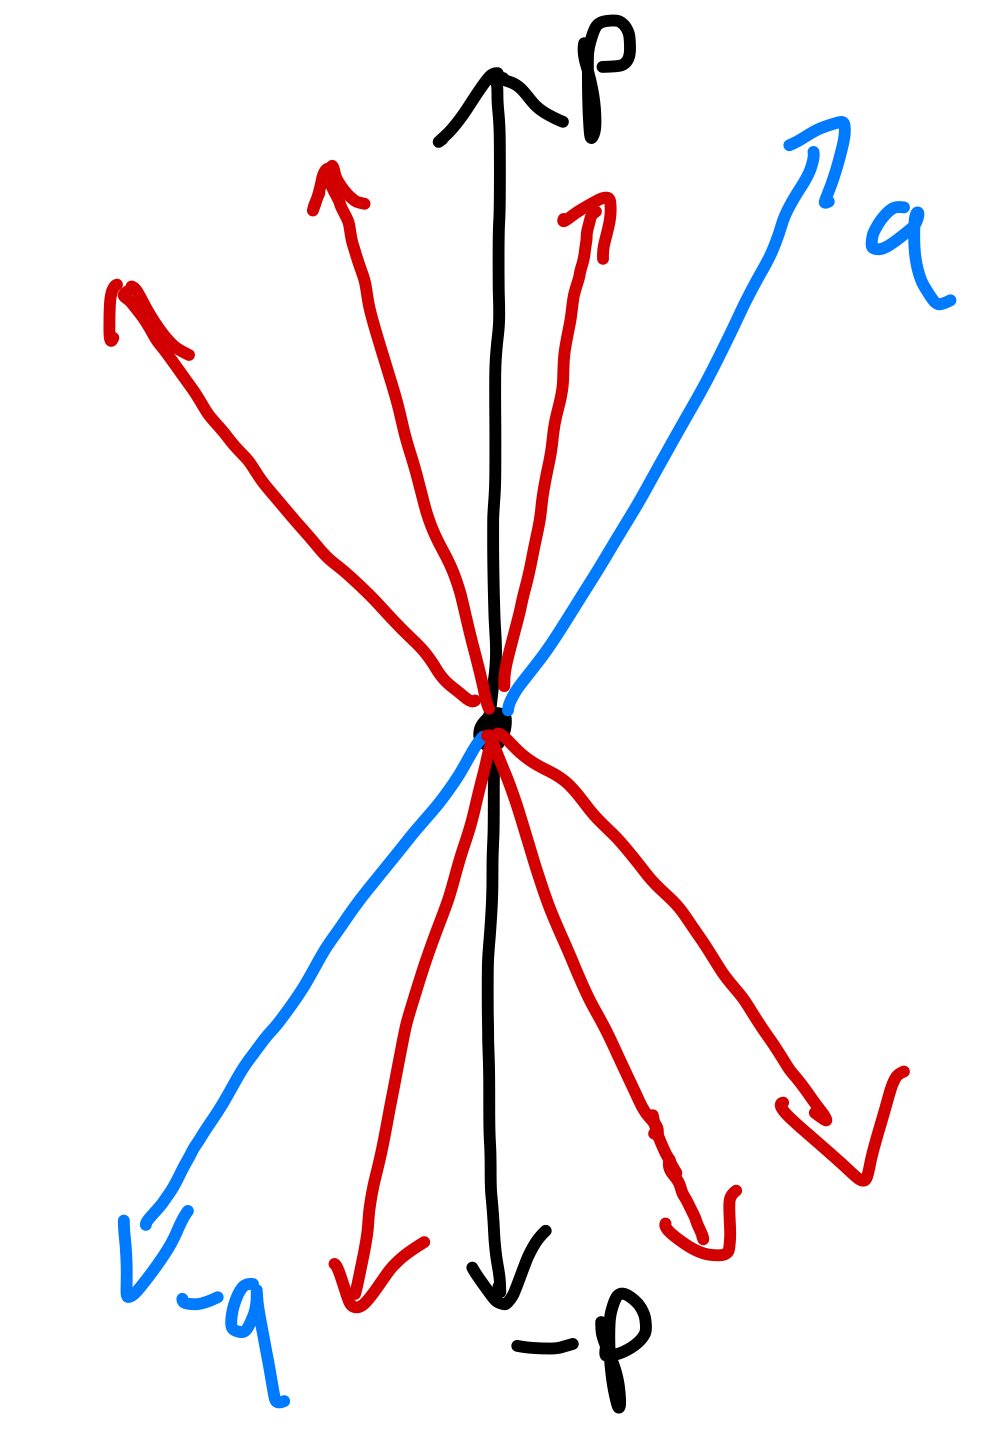
\includegraphics[width=4cm]{Lecture Files and Images/lec18-wrongpoles.png}
\end{center}
Now, let's try to figure out the other 4 poles in our orbit. Suppose we draw $q$ such that $p$ and $q$ are not perpendicular.
For any $q$ in the orbit, $-q$ is also in the orbit. We have determined that rotations by $\pi/2$ around $p$ are in our group, so those rotations of $q$ should also be in our orbit. However, this gives us 4 vectors for rotations of $q$ and 4 vectors for rotations of $-q$, and this is too many. 
This picture was wrong because $q$ was not drawn perpendicular to $p.$ If we drew $q$ perpendicular, then rotating $q$ by 90 degrees gives us an orbit of size 6. 

\begin{center}
    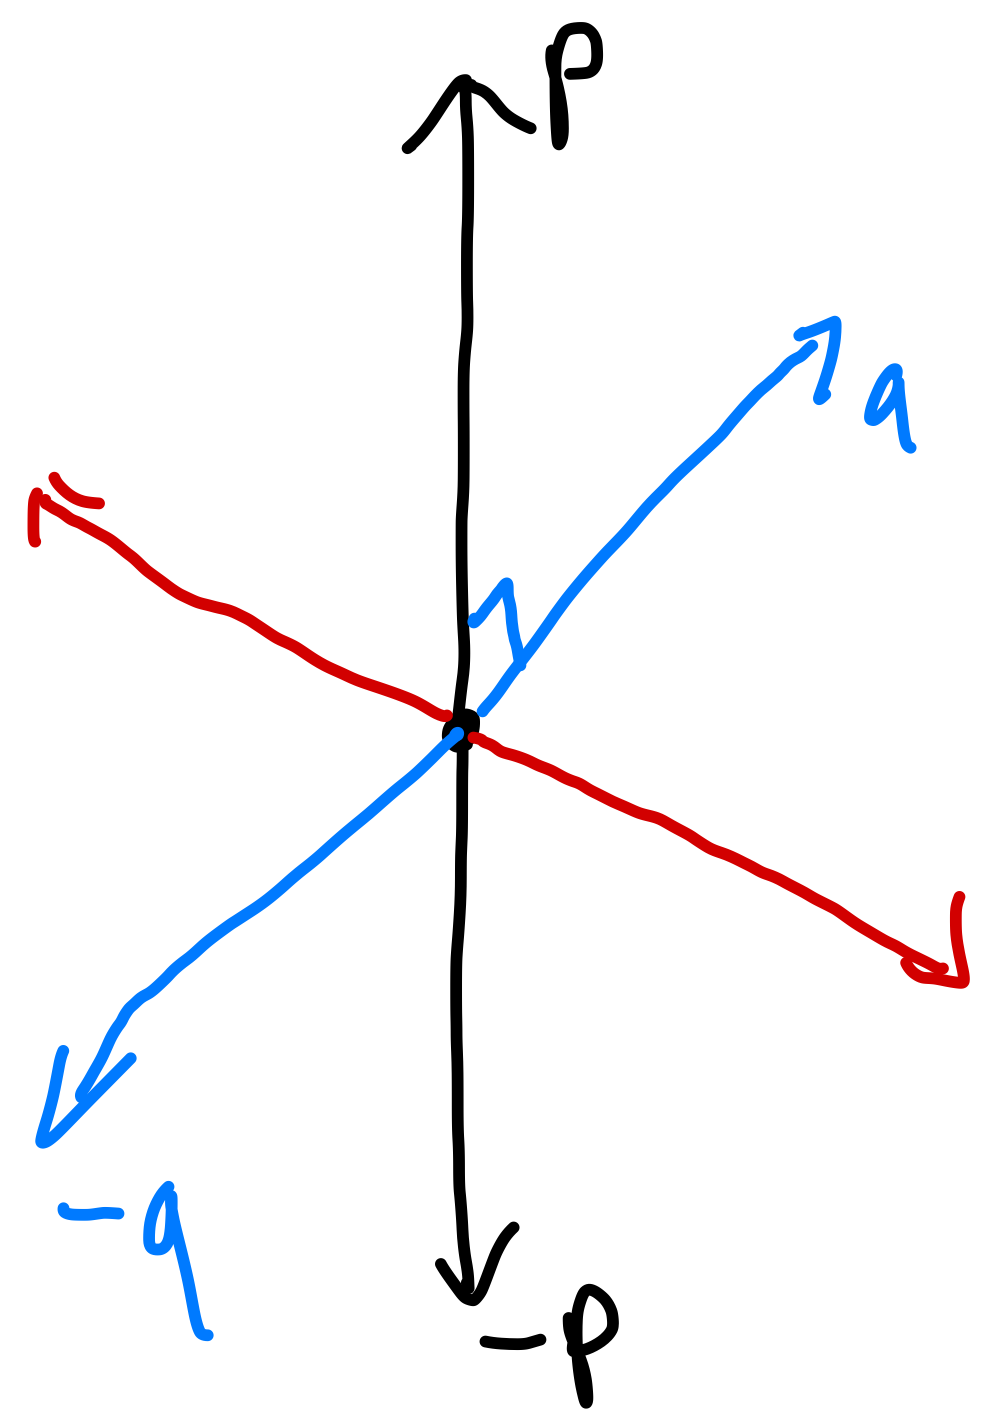
\includegraphics[width=4cm]{Lecture Files and Images/lec18-rightpoles.png}
\end{center}
Whatever the group $G$ is, it fixes the collection of vectors that we drew. In particular, it fixes the octahedron obtained by taking the convex hull of the vectors and thus $G\leq O$. But the octahedral group has size 24\footnote{we worked this out in class on Wednesday} and this group also has size 24, so $|G| = |O| = 24$ implies that $G = O.$

%37:11
\end{example}

We can repeat this for all the cases to finish the proof, but it isn't too important. 
The key lesson is how we were able to use the counting formulas and orbit decomposition of the set to really constrain the possibilities in these ways.
A lot of the challenge was just finding the right set to act on; in this case it was the poles. 

% \begin{question}[Student Question]
% The number of discrete symmetry group s is less than the number of Platonic solids; this is because some of the polyhedra have the same symmetry groups! For example, the dodecahedron and the icosahedron have the same symmetry group $G;$ this is because they are "duals" of each other by replacing faces by vertices. Did this just happen as a coincidence or is there any way to predict it?
% \end{question}
% ethany: idk lol
\newpage

\lhead{Lecture 19: Group Actions on $G$}
\setcounter{section}{18}
%MIT OpenCourseWare: https://ocw.mit.edu
%RES.18-011 Algebra I Student Notes, Fall 2021
%License: Creative Commons BY-NC-SA 
%For information about citing these materials or our Terms of Use, visit: https://ocw.mit.edu/terms.

\section{Group Actions on $G$}
\subsection{Conjugation}
Today, we will discuss the special case of group actions where the set $S$ is $G$ itself. 
We've seen the power of studying orbits and stabilizers and how they can help us understand groups of symmetries. 
One attempt is to just directly apply the group action on $G$:
\begin{align*}
    G \by G &\rto G \\
    (g, x) &\mto gx.
\end{align*}
However, this isn't particularly interesting. The action is transitive, and thus there is only one orbit and the stabilizers are all trivial. 

We instead define a different group action on itself, \textbf{conjugation}. It takes 
\begin{align*}
    G \by G &\rto G \\
    (g, x) &\mto gxg^{-1},
\end{align*}
conjugating $x$ by $g.$ 
One can check that it satisfies the axioms of a group action. %maybe do it?
We have some special names for the orbit and stabilizer under conjugation.
\begin{definition}
The orbit of an element under conjugation is 
\[C(x) \coloneqq \text{Orbit}(s) = \{gxg^{-1}: g \in G\},\]
and is called the \textbf{conjugacy class} of $x.$
\end{definition}

\begin{definition}
The stabilizer of an element under conjugation is 
\[
Z(x) \coloneqq \text{Stab}_G(x) = \{g \in G: gxg^{-1}=x\} = \{g \in G: gx = xg\} \leq G.
\]

It is called the \textbf{centralizer} of $x$ in $G,$ and it is a subgroup of $G.$ 
\end{definition}

From before, for \emph{any} $x \in G,$
 we have 
 \[
 |G| = |C(x)| \cdot |Z(x)|,
 \]
 and we also have the \textbf{class equation}, which states that 
 \[
 |G| = |C_1| + \cdots + |C_k|,
 \]
 since the conjugacy classes partition $G,$ and additionally, each $|C_i|$ divides $|G|$ from the counting formula.
 \begin{question}
    Are the conjugacy classes related to cosets, like we saw how left cosets of a subgroup partitioned a group?
 \end{question}
 \begin{ans}
    No, in general the conjugacy classes won't have the same size like cosets do. 
    We'll be seeing exactly what this equation looks like for different examples in the next few lectures. 
 \end{ans}
 
 Another related set, which we saw in homework before is the center of a group. 
 \begin{definition}
 The \textbf{center} of $G$ is 
 \[
 \{Z \coloneqq x \in G: xg = gx, g \in G\}.
 \]
 \end{definition}
 
 Other facts: 
 \begin{itemize}
     \item $C(x) = \{x\}$ is equivalent to $Z(x) = G$ and also $x \in Z,$ the center of $G.$
     
     So if we had an abelian group, then the center would be the whole group, and the class equation would be just the sum of a bunch of 1s.
     \item For any $x \in G,$ we have that $Z \leq Z(x)$ since the center commutes with all elements. Also, since $x$ commutes with itself, $\langle x \rangle \leq Z(x).$ This fact is a lower bound on the order of $Z(x)$, so it gives us the upper bound $|C(x)| \leq |G|/\ord(x)$.
     
     \item For all $x \in G,$ conjugation preserves order: $\ord(x) = \ord(gxg^{-1})$. This is true because conjugation defines an automorphism of our group. If $x^k = e$, then $e = gx^kg^{-1} = (gxg^{-1})^k$ so $x^k = e$ is equivalent to $(gxg^{-1})^k = e.$
 \end{itemize}
 
 
\begin{question}
Why is conjugation an automorphism?
\end{question}
\begin{ans}
We can just show that conjugation satisfies the homomorphism property, that it preserves products: $gxyg^{-1} = gxg^{-1}gyg^{-1}.$
Conjugation is a homomorphism and in fact an isomorphism from $G$ to itself. Since it is an automorphism of $G,$ elements that are conjugate to each other will have the same properties with respect to order; whether or not they commute; and so on. 
\end{ans}

All we have done so far is take observations about these definitions, and the class equation comes from our work on group actions from last week.

\begin{example}
What does the class equation say for $D_5$? The order of the group is $|D_5| = 10.$ It is equal to 
\[
D_5 = \{e, x, x^2, x^3, x^4, y, xy, x^2y, x^3y, x^4y\}.
\]

One of the properties of reflections is that conjugating $x$ by $y$ gives $yxy^{-1} = x^4.$
Let's figure out the conjugacy class of all the elements. 
The identity commutes with everything, so its conjugacy class is $C(e) = \{e\}.$ 

Now let's look at the reflection $y$.
From our facts above about the centralizer, we know that $\langle y \rangle \leq Z(y) \leq D_5.$ Then $Z(y)$ must be at least 2, and it must divide 10, so 2 and 10 are our only possibilities. 
However, not every element in $D_5$ commutes with $y,$ so $|Z(y)| = 2,$ and thus $|C(y)| = 5.$ In fact, every reflection is conjugate to every other reflection: $C(y) = \{\text{all reflections}\}.$ 

The conjugacy class of $x$ is at least $x$, and it is also at least $\{x, x^4\}.$ It cannot be more, because the order must divide 10 and we only have 4 elements left to partition. Then we have $C(x) = \{x, x^4\}$ and similarly $C(x^2) = \{x^2, x^3\}.$

So we have $10 = 1 + 5 + 2 + 2.$ 
The center corresponds to the elements that are in its own conjugacy class, so the center of $D_5$ is $\{e\}.$
\end{example}
Notice that the conjugacy classes have very different sizes; they partition the group in a very different way from cosets.

Since the group was small, we could have just brute forced and directly calculated the conjugacy classes for every element. However, looking at these divisibility facts is powerful and can handle more complicated and larger groups.
\begin{question}
The conjugacy classes seem to contain $x^{-1}$; is that always true?
\end{question}
\begin{ans}
In the example, it was specifically true because $yxy^{-1} = x^4$.
However, in general it isn't true.
For example, in the integers, $5$ and $-5$ are inverses, but not conjugate to each other.
\end{ans}
\subsection{\texorpdfstring{$p$}{p}-groups}

By studying the class equation, it is possible to gain some information about a general class of groups, $p$-groups.

\begin{definition}
$G$ is a $p$-group for a prime $p$ if $|G| = p^e$ for some $e \geq 0.$
\end{definition} 

There exists a group of any order simply by taking the abelian cyclic group of that order.
\begin{example}
For example, we have a $p$-group for every $e \geq 0$ by taking $C_p,$ $C_{p^{2}}$, $C_{p^3}$, and so on. Another example of a $p$-group is $C_p \times C_p \times \cdots \times C_p$.
\end{example}

Looking at a subgroup of $3 \by 3$ matrices also provides an example of a $p$-group.
\begin{example}
A more interesting group is the set of matrices
\[\begin{pmatrix}
1 & \star & \star \\
 & 1 & \star \\
 & & 1
\end{pmatrix} \leq GL_3(\FF_p),\]
which has order $p^3.$
\end{example}

By looking at the class equation modulo $p,$ the following theorem holds.

\begin{theorem}
Every $p$-group has non-trivial center.\footnote{There are elements of the center that are not the identity.}
\end{theorem}

\begin{example}
For $G = D_4,$ $|G| = 8 = 2^3.$ The class equation says $8 = 1 + 1 + 2 + 2 + 2,$ so the center has size 2 (since there are two 1's in the class equation.) %explain this better
\end{example}

\begin{proof}
The class equation for $G$ states that 
\[
|G| = |C_1| + \cdots + |C_k|,
\]
which is 
\[
p^e = (1 + \cdots + 1) + (p + \cdots + p) + (p^2 + \cdots + p^2) + \cdots + (p^{e-1} + \cdots + p^{e-1}),
\]
since the order of the conjugacy class must divide the order of $G.$

Recall that the sizes of the center, $|Z|$ is exactly the number of $1$s in the class equation. Then the equation taken modulo $p$ gives 
\[
0 = |Z| \text{ mod } p,
\]
which implies that $p$ divides $|Z|,$ since $|Z| \geq 1$ because at least the identity $e$ is in $Z.$ So $|Z| \geq p,$ and then the center is nontrivial.
\end{proof}

This theorem is interesting because we get some nontrivial information about the group \emph{just} from the size of the group, by using the class equation and looking at the numerics.

\begin{example}
Take the upper triangular matrices of the form \[\begin{pmatrix}
1 & \star & \star \\
 & 1 & \star \\
 & & 1
\end{pmatrix} \leq GL_3(\FF_p).\]

What is the center of the group? We want \[\begin{pmatrix}
1 & a & b \\
 & 1 & c \\
 & & 1
\end{pmatrix}
\begin{pmatrix} 1 & x & y \\
 & 1 & x \\
 & & 1
\end{pmatrix} = \begin{pmatrix}1 & x & y \\
 & 1 & x \\
 & & 1
\end{pmatrix}\begin{pmatrix}1 & a & b \\
 & 1 & c \\
 & & 1
\end{pmatrix}\] for all $x, y, z.$
This happens exactly when $a = c = 0$ and $b$ can be anything. So $|Z| = p,$ since there are $p$ possibilities for $b.$

\end{example}

The example above was a group of order $p^3$ having center of size $p$, so it demonstrates that there is not a better theorem where the center always has size $p^2,$ or something. 

However, we can say a little more about the specific case of $|G| = p^2$.
\begin{corollary}
If $|G| = p^2,$ then $G$ must be abelian.\footnote{Earlier on, we stated that if $p$ were prime, then $G$ must be cyclic; now we get from $p^2$ that $G$ is abelian, although not necessarily cyclic.} 
\end{corollary}

\begin{proof}
We have 
\[
\{e\} \lneq Z \leq G.
\]
We want to show that $|Z| = p^2,$ because that implies that $Z = G$ and then $G$ is abelian. We already know that $p$ divides $|Z|$, and that $|Z| \geq p,$ so the only two possibilities are $p$ and $p^2.$ Assume for the sake of contradiction that $|Z| = p.$ Then, pick $x \in G \setminus Z$ that is not in the center. Then, $Z \lneq Z(x)$; $Z(x) \neq Z$ because $x \in Z(x)$ but $x \not \in Z$. 
%30:03 

Then there exists $x \in Z(x)$ such that $x \notin Z.$ Thus if $|Z| = p,$ the only possibility is that $|Z(x)| = p^2$ since $Z(x)$ is a subgroup.
However, this implies that $Z(x) = G,$ but then $x \in Z,$ which is a contradiction. 
\end{proof}

The issue here is that $p^2$ is just not very big, so there is not very much room for a lot to happen.
We can even classify exactly what groups of size $p^2$ look like.
\begin{corollary}
Given a group $G$ such that $|G| = p^2$, $G$ must be isomorphic to either $C_{p^2}$, the cyclic group of size $p^2,$ or $C_p \by C_p = \{(a, b): a, b \in C_p\}$. 
\end{corollary}


\begin{proof}

We can split this up into two cases.
\begin{itemize}
    \item \textbf{Case 1.} If there exists $a \in G$ with $\ord(a) = p^2,$ then $\langle a \rangle = G,$ since $\langle a \rangle$ has size $p^2,$ and thus must be the entire group $G.$ 
    
    \item \textbf{Case 2.} Otherwise, every element $a \neq e$ has order $p,$ since it must divide $p^2$ and cannot be $p^2$ since we already considered that case. We claim that $G$ being abelian such that every $x \neq e$ has order $p$ comes from considering it as a vector space $V$ over $F = \FF_p$ %what does this mean??
    
    What is the dimension of this mystery vector space? The group $G$ has size $p^2,$ so it has dimension $p.$ So $V = F \oplus F$, implying that $G = C_p \by C_p.$ Here, we are forgetting the vector space structure and just thinking about it as a group with respect to addition.
    
    The addition structure is already implicit from the structure on $G.$ To turn $G$ into a vector space, we only need to define how to scale $g \in G$ by $\overline{n} \in \FF_p,$ and then check the vector space axioms. Let $\overline{n} \cdot g = \overbrace{g + \cdots + g}^{\text{n times}}$ This is well-defined because $\ord(g) = p,$ so it only matters what $\overline{n}$ is modulo $p.$
    We have figured out a way to turn the group into a vector space. Since any two vector spaces of the same dimension are isomorphic to each other as vector spaces; in particular, they are isomorphic to each other as abelian groups.

\end{itemize}

\end{proof}


All of this is gravy from what we were supposed to discuss this week, but it is helpful to see these examples.

\newpage

\lhead{Lecture 20: Class Equation for the Icosahedral Group}
\setcounter{section}{19}
%MIT OpenCourseWare: https://ocw.mit.edu
%RES.18-011 Algebra I Student Notes, Fall 2021
%License: Creative Commons BY-NC-SA 
%For information about citing these materials or our Terms of Use, visit: https://ocw.mit.edu/terms.

\section{The Icosahedral Group}

\subsection{Review: The Class Equation}
Last time, we discussed the conjugacy class of an element, which is the orbit of an element under conjugation, and the centralizer of an element, which is the stabilizer of an element under conjugation. 
\begin{definition}
The \textbf{conjugacy class} of an element is 
\[
C(x) \coloneqq \{gxg^{-1} : g \in G\} \subseteq G.
\]
\end{definition}

\begin{definition}
The \textbf{centralizer} of an element is 
\[
Z(x) \coloneqq \{g: gxg^{-1} = x\} \leq G.
\]
\end{definition}

The \textbf{class equation} states that 
\[
|G| = |C_1| + \cdots + |C_k|,
\]
which tells us information about a group simply through numerics.

\subsection{Basic Information}
The group $I \leq SO_3$ is the icosahedral group, which is the group of symmetries of the icosahedron under rotations (orientation-preserving isometries in $\RR^3$.) It is isomorphic to the dodecahedral group.

The group is \[I = \{\rho_{(u, \theta)}\},\] where each $\rho_{(u, \theta)}$ is a rotation by $\theta$ around a vector $u$ preserved by the rotation, which is called a \emph{pole} of $u.$ Additionally, the rotations have the property that $\rho_{(u, \theta)} = \rho_{(-u, -\theta)}.$ For a polyhedral group, $u$ lies on a face, an edge, or a vertex of the polyhedron. 

Let's start with counting the number of rotations in $I$ by whether the pole is on a face, an edge, or a vertex.

\begin{center}
    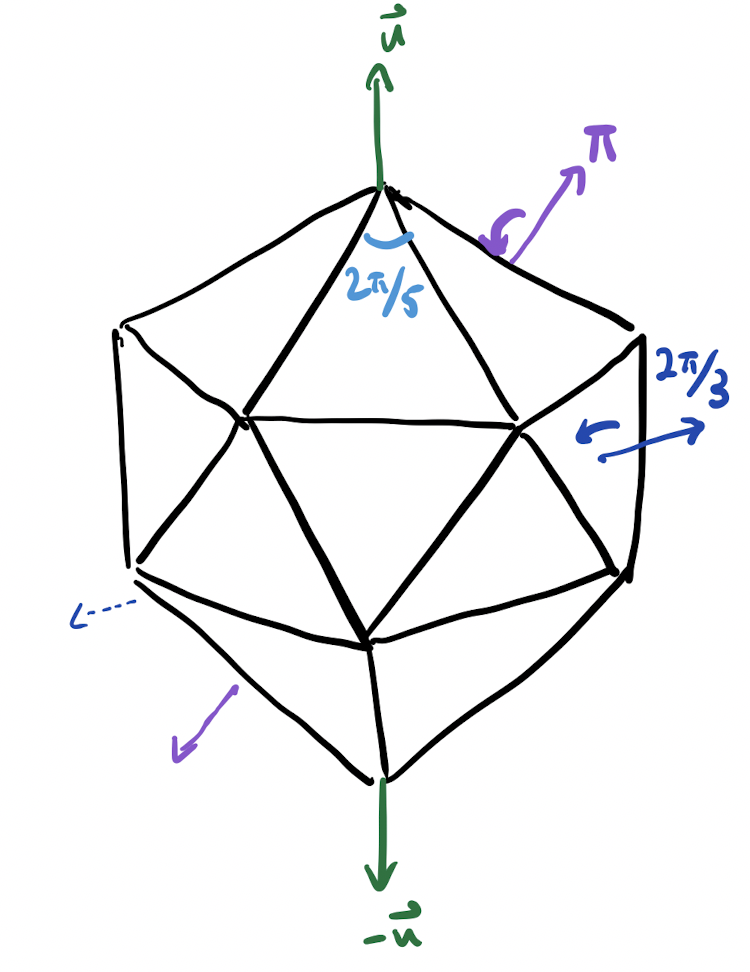
\includegraphics[width=7cm]{Lecture Files and Images/lec20-icos.png}
\end{center}

\begin{itemize}
    \item \textbf{Identity.} The trivial rotation is one rotation. 
    \item \textbf{20 faces.} For each face, excluding the identity, there are 2 rotations by $2\pi/3$ and $4\pi/3,$ which is 40 rotations total. In this way, every rotation is counted twice, since $\rho_{(u, \theta)} = \rho_{(-u, \theta)},$ 
    and every pole through the center of a face also goes through the opposite face. So we count 20 face rotations total.
    
    \item \textbf{30 edges.} For each face, there is one (non-identity) rotation by $\pi,$ and this also gets double-counted, so there are $30/2 = 15$ edge rotations total. 
    
    \item \textbf{12 vertices.} For each vertex, there are four nontrivial rotations, by $2\pi/5, 4\pi/5, 6\pi/5,$ and $8\pi/5.$ This double-counts as well, so there are $12 \cdot 4 / 2 = 24$ total vertex rotations.
\end{itemize}

In total, we have $1 + 20 + 15 + 24 = 60$ rotations. 
\subsection{Conjugacy Classes}

Now, it is possible to understand $I$ by thinking about the group action of conjugation on itself.
\begin{qq}
How can we decompose $I$ into conjugacy classes and what does the class equation tell us about normal subgroups of $I$? 
\end{qq}

For $g \in I,$ the conjugate of $\rho_{(p, \theta)}$ under $g$ is $g\rho_{(p, \theta)} g^{-1} = \rho_{(q, \theta)}$, where $q = g(p),$ since conjugating by $g$ is essentially taking a change of coordinates by $g.$ Thus, the rotations by the same angle $\theta$ with poles that can be reached from each other, through conjugation by some element in $I$, are conjugate. Then, we can count the conjugacy classes. 
\begin{itemize}
    \item The identity is conjugate to itself.
    
    \item Thus, the face rotations by $2\pi/3$ are all conjugate.\footnote{These are the same as the face rotations of $4\pi/3$; one angle must be picked to avoid double-counting.} 
    
    \item In addition, the vertex rotations by $2\pi/5$ (or $8\pi/5 = 2\pi - 2\pi/5$; they are the same rotation with the pole flipped) are conjugate.
    
    \item The vertex rotations by $4\pi/5$ and $6\pi/5$ are conjugate as well. 
    
    \item The edge rotations are all conjugate. 
\end{itemize}

Then the class equation states that 
\[
60 = 1 + 20 + 12 + 12 + 15.
\]

In particular, we see that the center of the group is trivial.

\subsection{Simple Groups}
We can use the class equation to study normal subgroups of $I.$ The following definition and then analysis provides one way the class equation can be useful.

\begin{qq}
How can we study complicated groups by decomposing them into simpler groups? 
\end{qq}

\begin{definition}
A group $G$ is \textbf{simple} if the only normal subgroups $H \nsub G$ are $H = \{e\}$ or $H = G.$\footnote{A group $G$ always has at least two subgroups, the trivial subgroup and the whole group, and a simple group only has these two.} Equivalently, $G$ is simple if for any surjective homomorphism $f: G \rto G'$, $G' = G$ or $G' = \{e\}.$\footnote{Since the kernel of the homomorphism is a normal subgroup, the kernel must be either $\{e\}$ or $G,$ leading to these two cases: either $f$ is an isomorphism or $f$ is trivial.}
\end{definition}

The guiding principle for studying groups is that simple groups are building blocks for all finite groups. To study a complicated group $G,$ it is possible to break it up by considering surjective homomorphisms to a smaller group $G'$ and studying instead the kernel, which is normal, and the image, which is $G'.$ Once a simple group is reached, there are no more interesting surjective homomorphisms, and in this way a group can be "decomposed" into simple groups.

For example, $C_n$ is simple if and only if $n$ is prime. In the same way that primes are building blocks for integers, simple groups are building blocks for all finite groups and cannot really be broken down any further.

\begin{question}
Does this mean that $p$-groups are simple? 
\end{question}

\begin{ans}
No. For instance, any subgroup of an abelian group will be normal, so an abelian group containing any nontrivial subgroup will not be simple. In particular, $C_{p^n}$ for $n \neq 1$ are not simple. The center of a subgroup is always a normal subgroup, and the center of a $p$-group is nontrivial, so whenever the center of a $p-$ group is not the entire group, the $p$-group will not be simple.
\end{ans}

\begin{theorem}
The icosahedral group $I$ is simple.\footnote{It has no normal subgroups.}
\end{theorem}

\begin{proof}
If $N \nsub I,$ then $gNg^{-1} = N.$ In fact, for some element $x \in N,$ its conjugate $gxg^{-1} \in N$ as well. Thus, for $x \in N,$ $C(x) \subseteq N$ as well. So the normal subgroup is a union of conjugacy classes:
\[
N = \bigcup_{x_i \in N} C(x_i).
\]

Also, $|N|$ divides 60 for $G = I.$ Since $60 = 1 + 20 + 15 + 12 + 12,$ we must have that $1 + $ (a subset of $\{20, 15, 12, 12\}$) is a factor of 60, which is possible only when $|N| = 1$ or $60,$ in which case $N = \{e\}$ or $I.$ So there are no other normal subgroups of $I,$ and $I$ is simple.
\end{proof}

In some sense, this is a very soft proof. We do not really have to grapple with the group structure of the mystery normal subgroup $N;$ all we have to deal with is the sizes of the conjugacy classes. 

This argument is very special to $I$ and would not work for $D_5.$ On the other hand, it is still possible to list all of the normal subgroups of $D_5$ by looking at the class equation; there are not that many.

\begin{problem}
Try to follow the same proof for $D_5$ (and fail!)\footnote{Since it is not actually simple, the proof will not work.}
\end{problem}

Recall that $|S_5| = 5! = 120.$ Then, let $A_5$ be the subgroup of even permutations in $S_5;$ it is the kernel of the homomorphism  $\text{sign: } S_5 \rto \{\pm 1\}$, and has index 2, so it has order 60. 

\begin{theorem}
The icosahedral group $I$ is isomorphic to the alternating group $A_5.$ 
\end{theorem}

\begin{proof}
We want to show that an element in $I$ acts in the same way as an element of $S_5.$. To do this, we construct an action of $I$ on a set of size 5. 

We want to find a set $S$ such that the group action of $I$ on $S$ gives a homomorphism
\[I \xrightarrow[]{\text{non-trivial } f} S_5.\]

\begin{center}
    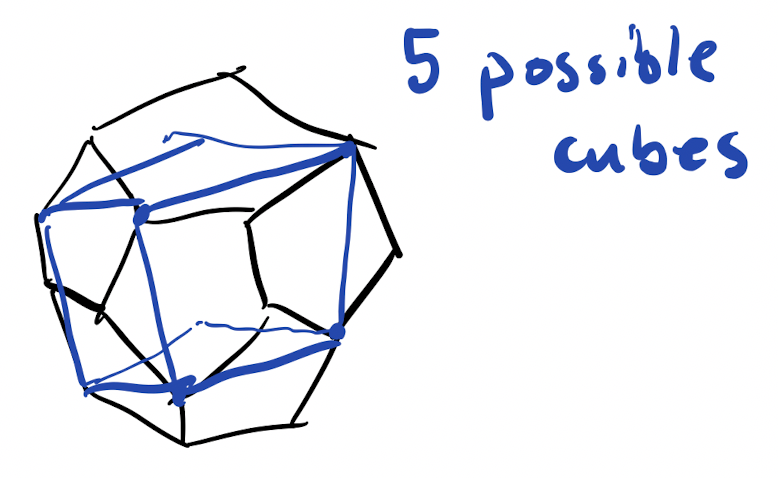
\includegraphics[width=7cm]{Lecture Files and Images/lec20-dodec.png}
\end{center}

Recall from before that $I$ is the symmetry group of both the icosahedron and the dodecahedron. There are five cubes fitting in the dodecahedron where the vertices are vertices of the dodecahedron and the edges of the cubes are diagonals of the pentagons that are the faces of the dodecahdron. For such a cube, every face of the dodecahedron will contain exactly one edge of the cube. Once one diagonal on one face is chosen, it determines the rest of the cube, and since a pentagon has five diagonals, there are 5 such cubes. 

Let $S$ be the set of $5$ cubes in the dodecahedron, labeled from 1 to 5 in some order. Then, $I$ clearly acts on $S,$ since it acts on the dodecahedron. 

Let 
\[
f: I \xrightarrow[\text{non-trivial}]{} \perm(S) = S_5
\]
take an element of $I$ to the corresponding permutation of the five cubes.

The group $I$ is simple, and the kernel of a homomorphism is always normal, so $\ker(f) \nsub I = \{e\}$ or $I.$ Since $f$ is nontrivial, $\ker(f) \neq I,$ so $\ker(f) = \{e\}.$ This implies that the homomorphism $f$ must be injective. 

Then, consider a different homomorphism $\varphi$ taking $I \rto \{\pm 1\}$, the composition
\[
I \xrightarrow[]{f} S_5 \xrightarrow[]{\text{sign}} \{\pm 1\}.
\]

Again, $\ker(\varphi) = \{e\}$ or $\ker(\varphi) = I.$ Since $|I| = 60 > |\{\pm 1\}| = 2,$ $\varphi$ is mapping a larger group onto a smaller group and cannot be injective, so $\ker(\varphi) = I.$ So under $\varphi,$ every element of $I$ maps to 1. However, this implies that the sign of the corresponding permutation of some element of $I$ is 1, so the corresponding permutation is even, and so $f(I),$ a subgroup of permutations in $S_5,$ consists entirely of even permutations. Then $f(I) \subseteq \ker(\text{sign}) = A_5,$ so $f$ is actually a homomorphism from $I$ to $A_5 \subset S_5;$ since it is injective from $I$ to $S_5,$ it is still injective from $I$ to $A_5.$ Since $I$ and $A_5$ are both of order 60, $f$ is also a surjection, and thus $f$ is an isomorphism between $I$ and $A_5$. 
\end{proof}

Throughout this proof, the fact that $I$ is simple is used over and over again to argue facts about various homomorphisms coming from $I.$

\begin{corollary}
The alternating group $A_5$ is also simple.
\end{corollary}

In fact, $A_n$ is simple for all $n \geq 5,$ but the proof is more complicated and involves thinking about the actual permutations. For the proof that $A_5$ is isomorphic to $I$ and thus simple, the class equation was the jumping-off point. The class equation showed that $I$ was simple, which then provided strong restrictions on homomorphisms from it. 

\subsection{Conjugacy Classes for Symmetric Groups}

Next time, the conjugacy classes for $S_n$ and $A_n$ will be determined. Recall that every $\sigma \in S_n$ can be decomposed via cycles. 
\begin{example}
The permutation $(123)(45) \in S_6$ takes $1 \mapsto 2,$ $2 \mapsto 3,$ and $3 \mapsto 1$ as the first cycle, of length 3, then $4 \mapsto 5$ and $5 \mapsto 4$ as the second cycle, of length 2, and $6 \mapsto 6$ as the third cycle, of length 1. 
\end{example}

The \textbf{sign} of $\sigma$, where $\sigma = \tau_1 \cdots \tau_r,$ where each $\tau_i$ is a 2-cycle\footnote{Also called a transposition.}, is $(-1)^r.$ For example, the sign of $(1234) = (12)(13)(12)$ is $-1.$ 

\newpage

\lhead{Lecture 21: Symmetric and Alternating Groups}
\setcounter{section}{20}
%MIT OpenCourseWare: https://ocw.mit.edu
%RES.18-011 Algebra I Student Notes, Fall 2021
%License: Creative Commons BY-NC-SA 
%For information about citing these materials or our Terms of Use, visit: https://ocw.mit.edu/terms.

\section{Conjugacy Classes for Symmetric and Alternating Groups}

\subsection{Review}

Recently, we have been discussing the conjugation action of a group on itself. In particular, it is possible to decompose a group into its \textbf{conjugacy classes}, which is similar to decomposing a set into its orbits (like we were doing last week).

Last time, we looked at the icosahedral group and saw its class equation and figured out information based on that.

\subsection{Cycle Type}
Today, we will be looking at the conjugacy classes for $S_n$ and $A_n,$ the symmetric group and the alternating group, which consists of even permutations. 

Recall that a permutation $\sigma \in S_n$ can be written in cycle notation. This is a very useful way of writing a permutation.

\begin{example}[Cycle Notation]
For example, the permutation $(123)(45)$ takes 1 to 2 to 3 to 1, and 4 to 5 back to 4. 
\end{example}

Given the cycle type, it is easy to define and figure out the \emph{sign} of a permutation. A $1$-cycle will have sign $+1$, a $2$-cycle will have sign $-1$, and so on, where a $k$-cycle will have sign $(-1)^{k-1}.$ For example, $(123)(45)$ has sign $-1 = (+1)(-1) = -1,$ where the signs of each cycle are multiplied. In particular, even permutations are permutations that have an even number of even-length cycles.\footnote{It's confusing: an even-length cycle makes a permutation odd.}

\begin{qq}
What are the conjugacy classes of $S_n$?
\end{qq}

It turns out that the sign will be a very helpful tool in determining the conjugacy classes. 

% An equivalent formulation has that the sign can also be determined from writing a permutation as a product of transpositions.

% \begin{definition}
% The \textbf{sign} of a permutation $\sigma = \tau_1\cdots \tau_k$ is $(-1)^k$ where each $\tau_i$ is a transposition. 
% \end{definition}

Let's look at an example.
\begin{example}
 If $\sigma = (123),$ then for $p \in S_n,$ let the conjugate be \[\tau = p\sigma p^{-1}.\] 
 
 Let's say $p(1) = i, p(2) = j,$ and $p(3) = k.$ Evaluating the conjugate on $i$ gives \[\tau(i) = p\sigma p^{-1}(p(1)) = p(\sigma(1)) = p(2) = j.\] Similarly, \[\tau(j) = p(\sigma(2)) = p(3) = k.\] It turns that in cycle notation, \[\tau = (ijk) = (p(1) p(2) p(3)).\] 
\end{example}

It is easy to check that $\tau$ fixes all the other points. So conjugating a 3-cycle produces another 3-cycle with different points. 

Consider a more complicated permutation. 
\begin{example}
For $\sigma = (123)(47) \cdots $, conjugating by $p$ gives \[(p(1)p(2)p(3))(p(4)p(7)) \cdots .\] 
\end{example}

It turns out that the lengths of the cycles in a permutation don't change upon conjugation! 

\begin{definition}
Given $\sigma \in S_n,$ the \textbf{cycle type} of $\sigma$ is the number of 1-cycles, 2-cycles, and so on, that show up in the cycle notation. 
\end{definition}

The cycle type is conjugation-invariant. If $\tau = p\sigma p^{-1},$ then $\sigma$ and $\tau$ have the same cycle type. For example, $(47)(123)$ has cycle type $(2, 3).$ 

In fact, if $\sigma$ and $\tau$ have the same cycle type, then they are conjugate. 

\begin{example}
Take \[\sigma = (1 4 5)(2 3)\] and \[\tau = (2 3 4) (1 5).\] Simply by matching cycles, we can define $p \in S_n$ taking $1 \mto 2,$ $4 \mto 3,$ $5 \mto 4,$ $2 \mto 1,$ and $3 \mto 5;$ that is, $p = (12)(354).$ This $p$ is constructed to be such that \[p\sigma p^{-1} = \tau.\footnote{Try working through this by hand!}\]
\end{example}

The upshot is this proposition. 
\begin{proposition}
Two permutations $\sigma$ and $\tau$ are conjugate if and only if $\sigma$ and $\tau$ have the same cycle type.
\end{proposition}

\subsection{Conjugacy Classes in $S_n$}

Conjugation in $S_n$ can be understood well by looking at cycles.

\begin{qq}
What are the conjugacy classes in $S_n$?
\end{qq}

From our characterization of when two permutations are conjugate, this can certainly be done! Let's start with an example.
\begin{example}
For $S_3,$ there are three conjugacy classes: cycle type $3, 2 + 1,$ and $1 + 1 + 1.$ For example, representatives could be $(123), (12),$ and the identity permutation. 
\end{example}

Now, we can do more complicated computations. For instance, we may want to find out the \emph{size} of a given conjugacy class.

\begin{example}[Conjugacy classes in $S_4$]
For a permutation \[x = (1234) \in S_4,\] the conjugacy class $C(x)$ is all $4-$cycles in $S_4.$ For each 4-cycle, there are 24 orderings of $1, 2, 3,$ and $4,$ and each one is overcounted by a factor of 4. For example, \[(1234) = (2341) = (3412) = (4123).\] So there are \[24/4 = \boxed{6}\] elements in the conjugacy class. 

Alternatively, where the stabilizer is $Z(x),$ then \[|C(x)| = \frac{|G|}{|Z(x)|}.\] Since conjugation is essentially "relabeling" the numbers in the original permutation, replacing 1 with $p(1),$ 2 with $p(2)$, and so on, the elements in the stabilizer should relabel the numbers $1$ through $n$ in such a way that the permutation is still the same. For instance, relabeling $(1234)$ to $(2341)$ gives the same permutation $x.$ In this case, because there are 4 different starting points to the cycle, there are 4 permutations $p \in Z(x)$ that stabilize $x.$ So again, \[|C(x)| = \frac{|G|}{|Z(x)|} = \frac{24}{4} = 6.\] Essentially, the redundancy in cycle notation gives us different ways to write the same permutation, and dividing out by this redundancy (the stabilizer) gives the size of the conjugacy class.
\end{example}

Cycle notation also simplifies these computations for larger symmetric groups.

\begin{example}[Conjugacy Class in $S_{13}$]
Consider \[x = (123)(456)(789 10)(11)(12)(13) \in S_{13}.\] What is the stabilizer $Z(x)$ of $x$? For the 4-cycles, there are 4 choices for where to start the cycle. Any reordering of 12, 11, and 13 doesn't change the fact that 12, 11, and 13 are fixed; there are $3!$ ways to order the 1-cycles. 

For the 3-cycles, there are 3 starting points each, but the 3-cycle $(123)$ could also be mapped to $(456),$ so there are 2! ways to order the two 3-cycles, and 3 starting points each. 

In general, if there are $k$ $\ell-$cycles, there are $\ell$ starting points for each cycle, and $k!$ ways to order them. So 
\[
|Z(x)| = 2!\cdot  3 \cdot 3 \cdot  4\cdot 3! \cdot 1 \cdot 1 \cdot 1 = 432.
\]

Then,
\[
|C(x)| = \frac{13!}{432}.
\]
\end{example}

So finding the sizes of conjugacy classes is really just doing some combinatorics for the size of stabilizer. Given the size of the stabilizer, since we know the size of the entire group, $|S_n| = n!$, dividing by $|Z(x)|$ directly gives $|C(x)|,$ without having to compute every permutation in the conjugacy class.

\subsection{Class Equation for S4}

Now, we can work out the class equation for $S_4$ without too much pain. 

\begin{example}[Class Equation for $S_4$]
The order of $S_4$ is $|S_4| = 4! =24.$ Then, there are only five possible cycle types, listed on the left column of the table. These are the different ways to sum to 4.


\begin{center}
    \begin{tabular}{c|c|c}
        cycle type & $|Z(x)|$ & $|C(x)|$ \\
        \hline 
        $4$ &  $4$ & 6 \\
        $3 + 1 $& 3& 8\\
        2 + 1 + 1 & $2\cdot 2!$ = 4 & 6 \\
        $2 + 2$ & $2! \cdot 2 \cdot 2 $= 8 & 3\\
        1 + 1 + 1 + 1 & 24 & 1.
    \end{tabular}
\end{center}

The size of the stabilizer for cycle type 4 is 4, as we worked out already. For 3, there are three possible places to start the cycle, so there are three permutations fixing the cycle type. For $2 + 1 + 1,$ there are 2 ways to pick a starting point for the 2-cycle and 2! = 4 ways to order the 1-cycles, which gives 4 total. The rest of the middle row follows similarly. 

We have \[|C(x)| = |G|/|Z(x)|,\] so the right row, the size of the conjugacy class, is found by dividing $|G| = 24$ by the middle row, the size of the stabilizer. 

The class equation then says 
\[
\boxed{24 = 1 + 3 + 6 + 8 + 6.}
\]
\end{example}

What about the alternating group? The conjugacy classes for $A_4$ can also be determined.
\begin{example}[Conjugacy classes for $A_4$]
What are the conjugacy classes for $A_4$?
\end{example}
The alternating group $A_4$ is a subgroup of $S_4.$ In fact it is the kernel of the sign homomorphism, so it is a normal subgroup. In particular, a normal subgroup is fixed under conjugation, so $A_4$ is the union of conjugacy classes. Using the definition of the sign, the cycle types $3 + 1,$ $2 + 2,$ and $1 + 1 + 1 + 1$ all correspond to the elements in $A_4.$ Then, taking the sizes of the corresponding conjugacy classes, we have
\[
|A_4| = 12 = 1 + 3 + 8,
\]
but since 8 is not a factor of 12, this is actually \emph{not} the class equation for $A_4.$ 

What's going wrong? If an element $\sigma$ is conjugate to another element $\tau$ in $A_4,$ it is a \textbf{different} notion than being $\sigma$ being conjugate to $\tau$ in $S_4$! In particular, $\sigma$ and $\tau$ can be conjugate in $S_4$, since we need $\tau = p\sigma p^{-1}$ for $p \in S_4,$ without being conjugate in $A_4,$ since we require that $\tau = q\sigma q^{-1} $ for $q \in A_4.$ If it is possible to find two elements conjugate by an odd permutation but not an even permutation, then they will be conjugate in $S_4$ but not $A_4.$ 

Consider $x \in A_n \leq S_n.$ The conjugacy class of $x$ in $A_n$ is \[C_A(x) = \{y \in A: y = pxp^{-1}, p \in A_n\},\] the subset of elements in $A_n$ conjugate to $x$ by some even permutation, which is a subset of 
\[
C_S(x) = \{y \in A_n : y = pxp^{-1}, p \in S_n\}.
\]

Similarly, the stabilizer for $A$ is a subgroup of the stabilizer for $S.$ 
\[
Z_A(x) = \{p \in A_n: px = xp\} \leq Z_S(x) = \{p \in S_n: px = xp\}.
\]

Using the counting formula,
\[
|C_A(x)| \cdot |Z_A(x)| = |A_n| = \frac{1}{2}|S_n|,
\]
so  
\[
|C_A(x)| \cdot |Z_A(x)| = \frac{1}{2}|C_S(x)| \cdot |Z_S(x)|.
\]

The product differs by a factor of 2 for $A_n$ and $S_n$. Additionally, $|Z_A(x)|$ is a factor of $|Z_S(x)|$, as it is a subgroup.

Our analysis leads us to two possibilities: 
\begin{itemize}
    \item \textbf{Case 1.} In this case, $|C_A(x)| = |C_S(x)|$ and $|Z_A(x)| = \frac{1}{2}|Z_S(x)|.$ Here, the conjugacy class stays the same size, but only half of the permutations that stabilize them are even and in $A_n.$ 
    
    \item \textbf{Case 2.} In this case, $|C_A(x)| = \frac{1}{2}|C_S(x)|$ and $|Z_A(x)| = |Z_S(x)|.$ So the size of the conjugacy class is split in half when going from $S_n$ to $A_n$, and only half of them are conjugate by even permutations. Since the sizes of the stabilizers of $x$ are the same, every $p \in S_n$ such that $px = xp$ is even, and lives inside of $A_n.$
\end{itemize}

In our example, 8 \emph{must} split, since it does not divide 12, and 1 and 3 cannot split because when they are split, they are split into halves, and they are odd numbers. Thus, the class equation for $A_4$ \textbf{must be}, by simple numerics,
\[
|A_4| = 12 = 1 + 3 + 4 + 4.
\]

In the $8 = 4 + 4$ case, $x = (123),$ and this is the case where the conjugacy class \emph{does} split, which means the stabilizer group does not get any smaller. Thus, every $p$ such that $px = xp$ is even. This is what it means for the stabilizer group not to get any smaller!

\begin{example}
What happens for $S_5$? What about $A_5$?
\end{example}

For $S_5,$ the class equation looks like 
\[
\boxed{120 = 1 + 10 + 15 + 20 + 20 + 30 + 24}.
\]

The even classes have size 1, 15, 20, and 24. We currently have \[|A_5| = 60 = 1 + 15 + 20 + 24,\] which is \textbf{not} the class equation. Clearly, 1 and 15 do not split, since they are odd. Since 24 is not a factor of 60 (but 24/2 = 12 is), it must split. 

The question remains if 20 splits into 10 + 10 or not. We can show directly that there is an odd permutation that commutes with it, and so it \emph{cannot} split. So the class equation is \[\boxed{60 = 1 + 15 + 20 + 12 + 12}.\]

These examples demonstrate that after our analysis of cycle types in symmetric and alternating groups, determining the class equation is not so much algebra and more counting and combinatorics.

\subsection{Student Question}
\begin{question}
Why do we care about $A_n$? Does it show up as the symmetry group of some object?
\end{question}

\begin{ans}
Since we are working with low numbers and dimensions, there are lots of coincidences where the groups that show up will be the same as each other, even if they aren't actually related in a general way for higher dimensions. In fact, $A_4$ shows up in the symmetry group of the tetrahedron, and we had $A_5$ show up as the symmetry group of the icosahedron. But in general, $A_n$ is (maybe? Davesh said he didn't really know/hadn't thought about it) not necessarily the symmetry group of some higher-dimensional geometric object. But in 18.702 we will study the symmetries of equations (Galois first studied these) instead of geometric objects, and it is very easy to write down equations that have $A_n$ or $S_n$ as (part of) their symmetry groups. In fact, group theory evolved at the same time as studying symmetries of non-geometric objects evolved (Galois again?) 

The reason why we care about $A_n$ is this idea that simple groups are "building blocks" in some sense, and $A_n$ for $n = 5$ and higher is simple, and in fact it is essentially the only (interesting?) simple normal subgroup of $S_n.$ So if we care about $S_n$ then we automatically care about $A_n,$ since $A_n$ is a "building block" of $S_n.$ 

In general, people like to break down problems into studying the simple subgroups of certain groups, and then studying the ways in which the simple groups can combine into the larger groups, in order to understand the larger group as a whole.

There are lots of ways of combining groups that get pretty complicated, and this is definitely something a lot of people are working on. The two ways of combining groups that get their own names are the "direct product" and the "semidirect product," which is a slightly more nonabelian way of combining groups. In this case, getting from $A_n$ to $S_n$ is just a semidirect product in some way.
\end{ans}

\newpage

\lhead{Lecture 22: The Sylow Theorems}
%MIT OpenCourseWare: https://ocw.mit.edu
%RES.18-011 Algebra I Student Notes, Fall 2021
%License: Creative Commons BY-NC-SA 
%For information about citing these materials or our Terms of Use, visit: https://ocw.mit.edu/terms.

\section{The Sylow Theorems}

\subsection{Review}

Last time, we discussed the conjugacy classes of symmetric and alternating groups.



\subsection{Motivation}

The Sylow theorems are a set of related theorems describing the subgroups of prime power order of a given finite group. They are very powerful, since they can apply to any finite group, and play an important role in the theory of finite groups. 

To motivate the Sylow theorems, recall the following basic theorem. 

\begin{theorem}\label{subgroup divisor}
If $G$ is finite, and $H$ is a subgroup of $G,$ then $|H|$ divides $|G|.$ 
\end{theorem}

In fact, we can ask if the reverse is also true: given a factor of $|G|,$ is there a subgroup of that size? It turns out that it it \textbf{not} true. 

\begin{example}[Counterexample]
For $G = A_4$, $|G| = 12$, but it turns out that there is no subgroup of order 6.\footnote{As an exercise, try showing this using the class equation!}
\end{example}

So there is not always such a subgroup. 

\begin{qq}
Can we add constraints so that some form of reverse of Theorem \ref{subgroup divisor} is true? When must there be a subgroup of a particular size?
\end{qq}

The next theorem is quite surprising and powerful: it turns out that the reverse is true for prime powers. If $d = p^k,$ a prime power dividing $|G|,$ then there must exist a subgroup where $|H| = p^k.$

\subsection{The First Sylow Theorem}

The three Sylow theorems, which will be stated in this lecture and proved in the next, formalize and elaborate on this idea of studying subgroups of prime power order. 

\begin{note}
For today's lecture, we use $e$ to denote the largest exponent of $p$ such that $p^e \mid |G|$ and we use 1 to denote the identity element instead. Also, $n$ will always refer to $|G|.$
\end{note}

The first Sylow theorem states that there is always a prime power order subgroup. 
\begin{theorem}[Sylow I]

Given $G$ such that \[|G| = n = p^e \cdot m,\] where $p^e$ is the largest power of $p$ (that is, $\gcd(p, m) = 1$), then there exists a subgroup $H \leq G$ such that \[|H| = p^e.\]
\end{theorem} 

Such a subgroup is called a \textbf{Sylow $p$-subgroup}. It has maximal prime power order within $G.$

\begin{definition}
Let $G$ be a group such that $|G| = n = p^e m$ such that $\gcd(p, m) = 1.$ Then a subgroup $H \leq G$ such that $|G| = p^e$ is called a \textbf{Sylow $p-$subgroup}.
\end{definition}

Let's see an application of this powerful theorem. 

\begin{example}
Consider $G = S_4.$ Since $|S_4| = 24 = 8 \cdot 3,$ Sylow I states that there is a subgroup of order 8. In fact, we can take \[H = \langle (12), (34), (13)(24) \rangle.\] 
\end{example}

Another example is the dihedral group. 

\begin{example}
For $G = D_5,$ we have $|D_5| = 10 = 2 \cdot 5.$ So there must be subgroups of size 5 and 2. A subgroup generated by a rotation
\[\langle \rho_{2\pi / 5} \rangle \text{ has order 5.}\] A subgroup generated by any reflection \[ \langle \text{reflection} \rangle \text{ has order 2.}\]
\end{example}

Looking at this theorem now, it may be hard to appreciate. One reason this theorem is relevant now is that the proof is a very nice application of the theory on group actions and orbits. Moreover, this theorem is one that applies extremely generally. We have mostly been studying explicit groups such as the dihedral groups or symmetric groups in this class, but the Sylow theorems apply to \textbf{any} finite group. When given an unfamiliar group, the Sylow theorems provide footholds and crevices, like in climbing a cliff, to start off with and to learn more about the groups. Sylow I gives lots of interesting subgroups that play off of each other, depending on the different factors of the size of the group $G.$ 

We can get a useful corollary for free. 

\begin{corollary}\label{cor of sylow i}
If $p$ divides $|G|,$ there exists an element $x \in G$ with order $p.$
\end{corollary}

For example, if $|G| = 14,$ it must have at least one element of order 7.

\begin{proof}[Proof of Corollary \ref{cor of sylow i}]

Using Sylow I, there exists a subgroup $H \leq G$ such that $|H| = p^e,$ where $e \geq 1.$ Pick some $y \in H$. Then, \[\langle y \rangle = C_{p^f},\] some cyclic group with order dividing $p^e$. Taking \[x = y^{p^{k-1}}\] provides an element of order $p.$
\end{proof}

\subsection{The Second Sylow Theorem}

The first Sylow theorem states that a Sylow $p$-subgroup, a subgroup of maximal size $p^e$ dividing $|G|,$ \textbf{exists}. In fact, we can say a lot more about what these subgroups look like.  

\begin{theorem}[Sylow II]
There are two parts; part a) is what is usually referred to as the second Sylow theorem.

\begin{enumerate}[label = (\alph*)]
    \item Given $H \leq G,$ where $H$ is a Sylow $p$-subgroup, any other Sylow $p-$subgroup $H' \leq G$ is conjugate to $H$; i.e. there exists $g$ such that $H' = gHg^{-1}$.
    
    \item Given any subgroup $K \leq G$ such that $|K| = p^d,$ for any Sylow subgroup $H,$ there exists $g$ such that $gKg^{-1} \leq H.$\footnote{Notice that $|K|$ does not have to be the maximal prime power, and can have order smaller than $|H|.$ \textbf{Every} prime power order subgroup, up to conjugation, sits inside a Sylow subgroup.}
\end{enumerate}
\end{theorem}

Evidently, conjugating a Sylow subgroup will result in a Sylow subgroup (since they have the same size), and Sylow II states that \textbf{all} the Sylow subgroups arise in this way. 

Note that the second part is stronger, since $|K|$ can be a prime power smaller than $|H|$, and implies the first part by applying b) to $K = H'.$ The second part states that given \textbf{any} prime power subgroup $K \leq G$ and \textbf{any} Sylow subgroup $H \leq G,$ it is possible to conjugate $K$ to make it land in $H.$

\begin{question}
Is the converse of part a) true? If $H$ is a Sylow $p$-subgroup, is $gHg^{-1}$ also a Sylow $p$-subgroup?
\end{question}
\begin{ans}
The converse is essentially automatically true. In order to be a Sylow $p$-subgroup, the only requirement is being a subgroup of a certain size, and conjugating by an element evidently produces a subgroup of the same size. The impressive part is that given two arbitrary Sylow $p$-subgroups, they must in fact be conjugate!
\end{ans}

Sylow II confirms our intuition for reflections in dihedral groups.
\begin{example}
For $D_{2n},$ every subgroup of size 2 is generated by a reflection, and Sylow II indicates that all the reflections are conjugate.
\end{example}

\subsection{The Third Sylow Theorem}

The last Sylow theorem indicates the number of these (conjugate) subgroups.

\begin{theorem}[Sylow III]
The number of Sylow $p$-subgroups of $G$ divides \[m = \frac{n}{p^e}\] and is congruent to 1 modulo $p.$
\end{theorem}

This theorem seems kind of weird, but is actually very useful.

\begin{example}
Consider $D_5$ and $p = 2.$ The number of Sylow $2-$subgroups is 5, which does divide $10/2$ and is congruent to 1 modulo 2.
\end{example}

The first Sylow theorem indicates \textbf{existence} of Sylow subgroups, the second Sylow theorem indicates that all Sylow subgroups are related by \textbf{conjugation}, and the third provides strong (and kind of funky) constraints on the \textbf{number} of such subgroups.



\subsection{Applications of the Sylow Theorems}

Now, we can look at a few different applications of these theorems, and we will see how powerful they are.

\begin{example}\label{order 15}
Consider any group $G$ such that \[|G| = 15 = 5 \cdot 3.\] 

By Sylow III, for $p = 5,$ the number of Sylow $5$-groups divides $3 = 15/5,$ and is equal to $1$ mod $5.$ In particular, the only possibility is \[\# \text{Sylow 5-groups} = 1.\] So there is a unique $H \leq G$ such that $|H| = 5.$ Since there is only one subgroup of size 5, Sylow II indicates that $gHg^{-1} = H.$ That is, $H$ is normal: the Sylow theorems indicate automatically that there is a normal subgroup of size 5.

For $p = 3,$ Sylow III states that the number of Sylow $3-$subgroups divides 5 and is 1 mod 3, so it is also 1. Thus, there exists some unique $K \nsub G$ such that $|K| = 3$.
\end{example}

Moreover, $H \cap K = \{1\},$ since $H \cong C_5$ and $K \cong C_3.$ Nontrivial elements of $H$ have order 5, while elements of $K$ have order 3, so they intersect only at the identity. So the Sylow theorems give, for free, nonintersecting normal subgroups of size 5 and 3 for \textbf{every single} group of size 15. That is quite impressive! 

Recall the notion of a \textbf{product group}.\footnote{This was discussed on the homework.}

\begin{definition}
The \textbf{product group} $H \by K$ is 
\[
H \by K = \{(h, k) : h \in H, k \in K\}
\]
where 
\[
(h, k) \cdot (h', k') = (hh', kk').
\]
\end{definition}

The product group is the group given by coordinate-wise multiplication. We claim that in Example \ref{order 15}, a group of order 15 must be isomorphic to a product of groups of order 3 and order 5.


\begin{proposition}[Example \ref{order 15}]\label{order 15}



Where $|H| = 5$ and $|K| = 3,$

 \begin{enumerate}[label = (\alph*)]
    \item the two subgroups commute: for $h \in H$ and $k \in K,$ $hk = kh$;
    \item $H \by K \cong G.$
\end{enumerate}
\end{proposition}

Once $H \by K \cong G,$ then we know that any group of order 15 is isomorphic to $C_5 \by C_3.$

\begin{proof}

Part b) follows from part a).

\begin{enumerate}[label = (\alph*)]
    \item For the first claim, since $K$ is normal, $hkh^{-1} \in K,$ and thus, multiplying on the right by an element of $K,$ \[hkh^{-1}k^{-1} \in K.\] Similarly, $kh^{-1}k^{-1} \in H,$ since $H$ is normal, but then \[hkh^{-1}k^{-1} \in H.\] Thus, $hkh^{-1}k^{-1} \in H \cap K = \{1\},$ and since the intersection was just 1, so $hkh^{-1}k^{-1} = 1,$ and so \[hk = kh.\]

\item Consider the mapping 
\begin{align*}
f: H \by K &\rto G \\
(h, k) &\mto hk.
\end{align*}

We claim that this is a homomorphism. In particular,
\[
f((h, k) \cdot (h', k')) = f((hh', kk')) = hh'kk' = hkh'k' = f((h, k)) \cdot f((h', k')),
\]
where the second-to-last step comes from $H$ and $K$ commuting.

In general, if we take two arbitrary subgroups and take this function, this would \textbf{not} be a group homomorphism! It was extremely important that $H$ and $K$ commute, which is true since they are both normal.

% In particular, $G$ could just be the cyclic group of size 15, and we have proven here that it is $C_5 \by C_3.$ 

Next, we must check that $f$ is in fact an isomorphism. Since $H$ and $K$ have trivial intersection, $hk = 1$ only when $h = 1$ and $k = 1,$ so the kernel is
\begin{align*}
\ker(f) &= \{h, k: hk = 1 \in G\} \\
&= \{(1, 1)\}.
\end{align*}

Since the kernel is trivial, $f$ is injective. In addition, $|H \by K| = |G| = 15,$ and so $f$ must be bijective and thus an isomorphism.

\end{enumerate}


\end{proof}

We have shown that any group $G$ of order 15 is
\[
G \cong C_5 \by C_3.
\] There is only one group of size 15. In particular, \[C_{15} = C_5 \by C_3.\]

\begin{question}
How did we know that $H$ and $K$ were $C_5$ and $C_3$?

\end{question}
\begin{ans}
Any group of prime order is cyclic; we proved this in a previous lecture.
\end{ans}

There is only one group up to isomorphism of order 15. For higher order groups, finding the number of groups up to isomorphism can get tricky. The Sylow theorems make it much easier to start an argument for classifying different groups, since they can apply to any finite group. 

For $n = 15,$ there is only one isomorphism class. 

\begin{qq}
For groups such that $|G| = pq,$ a product of two distinct primes, how many isomorphism classes of groups are there of size $pq$?
\end{qq}

Let's think about $n = 10.$

\begin{example}
Consider a group $G$ such that $|G|$ = $10 = 5 \cdot 2.$

\end{example} 

We know already that $G$ is not unique; for example, $D_5$ and $C_{10}$ both have order 10 but are non-isomorphic.

\begin{proposition}
There are two isomorphism classes: $G \cong C_5 \by C_2,$ and $G \cong C_{10}.$
\end{proposition}

\begin{proof}

From Sylow III, the number of Sylow $5$-groups divides 2 and is 1 modulo 5, so there is only one Sylow $5$-group. So there is a normal subgroup $K \nsub G$ such that $|K| = 5.$ Let $x \in K$ be a generator for $K,$ so that \[K = \langle x \rangle,\] where $\ord(x) = 5.$ 

Take $H$ to be some Sylow 2-group. Let $H = \langle y \rangle,$ where the order of $y$ is 2. Since $K$ is normal and generated by $x,$ $yxy^{-1}  \in K,$ so \[yxy^{-1} = x^r\]
for some exponent $1 \leq r \leq 4.$ Rearranged, we have \[yx = x^r y.\] 

As before, since $K$ has elements of order 5 and $H$ has elements of order 3, the intersection is trivial: \[K \cap H = \{1\}.\] This implies that the possible $x^iy^j$ are distinct from each other.\footnote{Otherwise, if there are two nondistinct elements, we end up with $x^{i-i'}y^{j-j'} = 1$, implying that some element of $K$ is the inverse of some element of $H,$ which is not possible with a trivial intersection.}

Therefore, the group $G$ is 
\[
G = \{x^i y^j: 0 \leq i \leq 4, 0 \leq j \leq 1\},
\]
where all these elements are distinct. There are 10 such elements, so these elements must be the entire group $G.$ The relations \[x^5 = y^2 = 1\] and \[yx = x^r y\] completely determine the group operation! The exponent $r$ entirely controls which group of size 10 we have. 

Which values of $r$ work? Currently, we have that $1 \leq r \leq 4,$ so there are \textbf{at most} four different isomorphism classes for $G.$ 

\begin{itemize}
    \item If $r = 2,$ then we would have \[x = y^2x = yyx = yx^2y = x^4y^2 = x^4,\] by repeatedly using the relations $x^5 = y^2 = 1; yx = x^r y$. Here we have $x = x^4$, implying that $x^3 = 1.$ This is a contradiction, since $x$ had order 5. So $r = 2$ is impossible.
    
    \item In general, if $yx = x^r y,$ then \[x = y^2x = \cdots = x^{r^2},\] by running through the same calculations as above. So $x^{r^2-1} = 1$, and we must have $r^2 = 1$ mod 5. So $r = 3$ is impossible, since $9$ is not 1 mod 5. 
    
    \item For $r = 1,$ then $H$ and $K$ commute by definition, and the same analysis as in \ref{order 15} works, and we have \[G = C_5 \by C_2,\] which turns out to be isomorphic to $C_{10}.$ 
    
    \item For $r = 4$, we recognize these relations: \[G = D_5.\]

\end{itemize}

For this example, we used the Sylow theorems to narrow down the possibilities, and simply looked through the possibilities to determine the isomorphism classes of groups of order 10. 

For $n = 10,$ because Sylow III did not restrict the number of $2$-subgroups to be 1, only the $5$-subgroup was necessarily normal, and so the analysis was more complicated and subtle than for $n = 15$. Since for $p = 2,$ there could have been 1 or 5 subgroups (both these numbers divide $10/2 = 5$ and are congruent to $1$ modulo 2), we were able to obtain less information about $2-$subgroups. 

\end{proof}

In general, if $|G| = pq,$ a product of two distinct primes, then 
\begin{itemize}
    \item if $q \neq 1 \mod p,$ then $G = C_p \by C_q = C_{pq}$.
    
    \item if $q = 1 \mod p,$ then $G = C_{pq}$ or a different non-abelian group.\footnote{For $p = 2$ and $q = 5,$ the different non-abelian group is $D_5.$}

\end{itemize}
To prove this, we follow the same analysis as today. The first step is to look at the Sylow $p-$groups and the Sylow $q-$groups. In the first case, we argue that they are normal and commute, and we can show that $G \cong C_p \by C_q.$ In the second case, using the relations, there end up only being two possibilities for $r.$

\newpage

\lhead{Lecture 23: Proving the Sylow Theorems}
%MIT OpenCourseWare: https://ocw.mit.edu
%RES.18-011 Algebra I Student Notes, Fall 2021
%License: Creative Commons BY-NC-SA 
%For information about citing these materials or our Terms of Use, visit: https://ocw.mit.edu/terms.

\section{Proofs and Applications of the Sylow Theorems}
\subsection{Review}
Last time, we introduced the Sylow theorems. While they may be a lot to take in, the main takeaway is how general the Sylow theorems are. When provided with \textbf{any} finite group, we automatically already know that there exist certain $p$-subgroups\footnote{The size is the largest power of $p$ that divides $|G|$} that must be conjugate, and additionally there is a strong constraint on the possible number of such subgroups.

The applications for $C_{15}$ and $C_{10}$ discussed last lecture demonstrate how powerful these theorems can be.

We restate the theorems briefly here:
\begin{theorem}[Sylow Theorems]
    Let $G$ be a finite group where \[|G| = n = p^em\] and $\gcd(p, m) =1$. The three parts of the theorem follow:
    \begin{enumerate}
        \item 
            Recall that a Sylow $p$-subgroup is a subgroup $H \leq G$ such that $|H| = p^e$. The first theorem states that there always exists a Sylow $p$-subgroup.
        \item 
            Given any $K \leq G$  where $|K| = p^f$, there exists some $g\in G$ such that $gKg^{-1} \leq H$.
        \item 
            The number of Sylow $p$-subgroups is a factor of $m$ and congruent to 1 mod $p$.
    \end{enumerate}
\end{theorem}

\subsection{Application: Decomposition of Finite Abelian Groups}
One application of the Sylow theorems is the decomposition of finite abelian groups. 

Consider a finite \emph{abelian} group $G$ such that the prime factorization of the order is \[|G| = p_1^{e_1} \cdots p_r ^{e_r}.\]

Then we know that we have a Sylow subgroup $H_i$ such that \[|H_i| = p_i^{e_i}\] for each of these primes. Since $G$ is abelian, conjugating a group produces the same group, so by Sylow II, these (abelian) subgroups $H_i$ are \textbf{unique} for each prime.

\begin{theorem}
Every abelian group $G$ is isomorphic to a product of groups of prime power order.
\end{theorem}

Using that $G$ is abelian, if we take the product \[H_1 \times \cdots \times H_r,\] we can construct a homomorphism\footnote{Because $G$ is abelian, we use + as the group operation.}
\begin{align*}
    f: H_1 \times \cdots \times H_r &\rto G \\
    (x_1, \ldots, x_r) &\mto x_1+ \cdots + x_r.
\end{align*}

\begin{lemma}
    The homomorphism $f$ is an isomorphism.
\end{lemma}


\begin{proof}
    First, $f$ is a homomorphism because $G$ is abelian and the terms will commute when verifying the homomorphism property. It is necessary that $G$ is abelian. \footnote{Essentially, since $G$ is abelian, there is really only one way to "combine" the Sylow $p$-subgroups. When $|G| = 10$ for a non-abelian group, we saw that the Sylow subgroups for 2 and 5 could combine in a different way to make $D_{10}.$} Next, we know that $\im(f)$ is a subgroup of $G$ and also contains a copy of $H_i$ for all $i$\footnote{Take $H_1 \by \{1\} \by \cdots \{1\}$ to get $H_1 \leq \im(f),$ for example.}: \[H_i \leq \im(f) \leq G\] for all $i.$
    Thus, $p_i^{e_i}$ divides $\lvert\im(f)\rvert$ for each $i$, and since they are relatively prime, the product 
    \[\prod p_i^{e_i}\] divides $\lvert\im(f)\rvert.$ This forces the image to be the same order as $|G|$, and thus they must be the same. We can conclude that $f$ is surjective. Both the domain and image of $f$ have the same size, so it is also injective and an isomorphism.
\end{proof}

As a result, the study of finite abelian groups can be reduced to studying abelian $p$-groups. These are completely understood, and will potentially be covered more in 18.702! In contrast, non-abelian groups are complicated and not well understood.

\subsection{Proof of Sylow Theorems}
The main idea to prove all of these theorems is to find a useful action of $G$ on a set and exploit it. This is a continuation of what we have been doing in the last few weeks, in geometric situations with symmetries as well as with the conjugation action of $G$ on itself. The striking part about these three proofs is that unlike rotational symmetries of the cube, where there are lots of sets to think about, such as vertices and faces and so on, here, there is no prior knowledge about $G$, and the only group action we have for any arbitrary group is $G$ acting on itself, and not much else. 

\begin{theorem}[Sylow I]

Given $G$ such that \[|G| = n = p^e \cdot m,\] where $p^e$ is the largest power of $p$ (that is, $\gcd(p, m) = 1$), then there exists a subgroup $H \leq G$ such that \[|H| = p^e.\]
\end{theorem}
\begin{proof}[Proof of Sylow I]
    Take $G$ such that \[|G| = p^e\cdot m.\]Let $S$ be the subsets of $G$ of size $p^e$ and let $n$ be the order of $G$. By basic combinatorics, there are $\binom{n}{p^e}$ such subsets, so \[|S| = \binom{n}{p^e}.\] Let $G$ act on $S$ by left translations: given an element $g \in G$ and a subset $U \in S$, we map \[U \mto gU.\]

    Our eventual goal is to find a subgroup of $G$ of size $p^e$ by looking at stabilizers, as they are always subgroups of $G.$ We find the size of a stabilizer by trying to find an orbit of size $m$, as we then know that the stabilizer will be order $p^e$.\footnote{The product of the size of an orbit and the size of the stabilizer is the size of the group $G,$ which here is $m \cdot p^e.$}
    We begin with some lemmas. The first lemma provides information about the size of the set modulo $p.$ 
    \begin{lemma}
    Where $n = |G| = m \cdot p^e,$ we have that \[|S| = \binom{n}{ p^e} \neq 0 \pmod{p}.\] Furthermore, \[\binom{n}{ p^e} \equiv m \pmod{p}.\] 
    \end{lemma}
    \begin{proof}[Sketch of Proof]
        The proof is not particularly relevant to group theory and can be proved by expanding the binomial coefficient and showing that the number of powers of $p$ in the numerator is the same as the denominator. Alternatively, one could expand $(1+x)^n$ and look at it modulo $p$.
    \end{proof}
    
    To reiterate, $S$ consists of \textbf{all} subsets of $G$ of size $p^e,$ and these subsets do not have to be subgroups. 
    
    \begin{lemma}
        Suppose we have a subset $U \in S$\footnote{Note that $U$ is an element of $S$ but is itself also a subset of $G$, so $U \subset G.$}, which is a subset of $G$. Also, let $H$ be a subgroup of $G$ that stabilizes $U$. Then, $|H|$ divides $|U|.$
    \end{lemma}
    \begin{proof}
        Since $H$ stabilizes $U$, for any $h \in H$, we know $hU = U$. In other words, for each $u \in U$, we have \[Hu \subset U.\] Equivalently, for each $u\in U$, the corresponding right coset of $H$ is a subset of $U$. This implies that the right cosets partition $U$. Since the cosets have the same size, we know that $|H|$ divides $|U|$. 
    \end{proof}

    With these lemmas in hand, we can continue with the proof of the main theorem. The first lemma tells us that $|S| \neq 0 \pmod{p}$. We know that the orbits partition $S$, so \[|S| = |O_1| + \cdots + |O_r|.\] Since $p$ does not divide the LHS, there must exist an orbit $\theta$ where \[\gcd(p, |\theta|) = 1.\] Let the size of $\theta$ be $|\theta| = k$. 
    
    Now, consider some element $u$ of $\theta$. By the counting formula, we also know that \[|G| = |\theta| \cdot \lvert\stab(u) \rvert.\] And so $p^em = k \lvert\stab(u)\rvert$ and $p^e \mid \lvert\stab(u)\rvert$ because $\gcd(k, p) = 1$. 
    By the second lemma, $\lvert\stab(u)\rvert$ divides $|u| = p^e$.

    Thus, \[\lvert\stab(u)\rvert = p^e\] and we have found a Sylow $p$-group.
\end{proof}

The proof of the second Sylow theorem is similar. 


\begin{theorem}[Sylow II]
There are two parts; part a) is what is usually referred to as the second Sylow theorem.

\begin{enumerate}[label = (\alph*)]
    \item Given $H \leq G,$ where $H$ is a Sylow $p$-subgroup, any other Sylow $p-$subgroup $H' \leq G$ is conjugate to $H$; i.e. there exists $g$ such that $H' = gHg^{-1}$.
    
    \item Given any subgroup $K \leq G$ such that $|K| = p^d,$ for any Sylow subgroup $H,$ there exists $g$ such that $gKg^{-1} \leq H.$\footnote{Notice that $|K|$ does not have to be the maximal prime power, and can have order smaller than $|H|.$ \textbf{Every} prime power order subgroup, up to conjugation, sits inside a Sylow subgroup.}
\end{enumerate}
\end{theorem}

\begin{proof}[Proof of Sylow II]
    We approach this proof similarly, finding a nice set and an action on it.
    Fix $H$ to be a Sylow subgroup.
    Our set is $X = G/H$, the left cosets of $H$. 
    The index of $H$ is the same as $|X|$, so $|X| = m$. 
    
    Let $K$ be the subgroup we want to show is a subgroup of $H$ up to conjugation, where $|K| = p^f$.
    We will look at how $K$ acts on $X$ by left translation, the mapping: $$k(aH) \mto kaH.$$

    We decompose into orbits, $|X| = |O_1| + \cdots + |O_r|$. 
    Note that these orbits are with respect to the action of $K$, not the action of $G$, as that would be transitive and we'd only have one orbit.
    We have that $|O_i|$ divides $|K| = p^f$, but $p$ does not divide $m$. 
    Thus this orbit decomposition can only work if some orbit $O$ has size 1. 
    In other words, there exists some coset $aH$ that is fixed by all $k \in K$. 
    Then,
    \begin{align*}
        kaH &= aH\\
        a^{-1}kaH &= H \\
        a^{-1} ka &\in H \\
        a^{-1}Ka &\leq H
    \end{align*}
    which is what we needed to show.
\end{proof}
A lot of the work done in these proofs are choosing some set and action, then looking at the orbits and seeing what we can do what them. The third proof is similar. 


\begin{theorem}[Sylow III]
The number of Sylow $p$-subgroups of $G$ divides \[m = \frac{n}{p^e}\] and is congruent to 1 modulo $p.$
\end{theorem}


\begin{proof}[Proof of Sylow III]
    Our set will be $Y$ as the set of Sylow $p$-subgroups of $G$. 
    We will be trying to find the size of $Y$.
    $G$ acts on $Y$ by conjugation, $H \mto gHg^{-1}$.
    By Sylow II, there is only one orbit. 
    Pick a Sylow subgroup $H \in Y$.
    Then $$|G| = \lvert\stab(Y)\rvert \lvert\text{orbit}(H)\rvert = |Y| \lvert\stab(Y)\rvert.$$
    This already tells us that $|Y|$ divides $|G| = n$, but we can say more.

    The stabilizer here has a name, the \emph{normalizer} of $H$. 
    It turns out that $H \leq  \stab(H)$ because for all $h \in H$, $hHh^{-1} = H$. 
    So $|\stab(H)|$ is divisible by $p^e = |H|$. 
    The counting formula then says that $|G| = p^em = |Y| \cdot (p^e \cdot \text{stuff})$ which implies that $|Y|$ divides $m$.

    The last part is showing that $|Y| \equiv 1 \pmod{p}$. 
    We now use the action of $H$ on $Y$ by conjugation. 
    \begin{fact}
        Suppose we have another Sylow subgroup $H' \in Y$, $H'$ is fixed by $H$ if and only if $H = H'$. 
        In other words, under the action of $H$, there is only one fixed point.
    \end{fact}
    By looking at orbits, there is only one orbit of size 1 because there is only one fixed point. 
    The rest are powers of $p$ because the size of $H$ is a power of $p$.
    Thus the decomposition into orbits looks like \[ Y = 1 + p + \cdots + p^2 + \cdots + p^3 + \cdots \equiv 1 \pmod{p}.\]

    \begin{proof}[Proof of fact]
        If we look at the stabilizer/normalizer, $\stab_G(H') = N(H')$, we know that $H \leq N(H')$ because $H'$ is fixed by $H$, and that $H' \leq N(H')$ by what we said above about normalizers. 
        
        Now $N(H')$ is a subgroup of $G$ as well, so the largest power of $p$ that divides $N(H')$ can only be $p^e$. 
        So $H$ and $H'$ are Sylow subgroups of $N(H')$ as well.
        By Sylow II on $N(H')$, there exists $n \in N(H')$ such that $nH'n^{-1} = H$. 
        But then by the definition of $N$, $nH' n^{-1} = H'$, and so $H = H'$. 
    \end{proof}
    
    Given this fact, we are done with the third proof.
\end{proof}

\newpage

\lhead{Lecture 24: Symmetric and Hermitian Forms}
%MIT OpenCourseWare: https://ocw.mit.edu
%RES.18-011 Algebra I Student Notes, Fall 2021
%License: Creative Commons BY-NC-SA 
%For information about citing these materials or our Terms of Use, visit: https://ocw.mit.edu/terms.

\section{Bilinear Forms}

\subsection{Review}
Last week, we talked about the Sylow theorems, which are fundamental to the theory of finite groups. 

\subsection{Bilinear Forms}
Throughout this class, we have been pivoting between group theory and linear algebra, and now we will return to some linear algebra.

Today, we will be discussing the notion of \textbf{bilinear forms}. Let's look at some examples first and then provide the general definition. 

For now, we will be working with a vector space $V$ over $F= \RR,$ and later on we will look at the case of $F = \CC,$ the complex numbers.

Let's consider three examples of bilinear forms on $\RR^3.$
\begin{example}\label{bilinear forms}

Consider these three different examples of mappings:
\begin{align*} \RR^3 \by \RR^3 &\rto \RR \\
\begin{pmatrix}
x_1 \\ x_2 \\ x_3
\end{pmatrix},
\begin{pmatrix}
y_1 \\ y_2 \\ y_3
\end{pmatrix} 
& \xmapsto{(1)} x_1y_1 + x_2y_2 + x_3y_3 \\
& \xmapsto{(2)} x_1y_1 + 2x_2y_2 + 3x_2y_1 + 4x_2y_3 + 5x_3y_1 \\
& \xmapsto{(3)} x_1y_1 + 2x_2y_1 + 2x_1y_2 + 3x_2y_2.
\end{align*}

\end{example}
These all take in pairs of vectors in $\RR^3$ and return a real number. They all have the property that when keeping the $y$'s fixed, the mapping is "linear" in the $x$'s, and when keeping the $x$'s fixed, the mapping is "linear" in the $y$'s.\footnote{The general idea of a bilinear form is that it is linear when varying in $x$ (and keeping $y$ fixed) and linear when varying in $y$ (and keeping $x$ fixed); hence, it is linear in two different variables, independently, so it is "bilinear." However, being bilinear is \emph{not} the same as being linear; for example, if both $x$ and $y$ were doubled, the output would quadruple.} In particular, there are no constant terms or terms that are squared or higher order in $x_i$ or $y_i$. 

\begin{definition}
A \textbf{bilinear form} is a function \begin{align*} V \by V &\rto \RR \\
(v, w) &\mto \langle v, w \rangle\footnotemark
\end{align*} 
\footnotetext{The angle brackets $\langle \cdot, \cdot \rangle$ are how a bilinear form is usually denoted.}
such that 
\begin{enumerate}
    \item $\langle v, cw \rangle = c\langle  v, w\rangle $ 
    \item $\langle v, w_1 + w_2 \rangle = \langle v, w_1 \rangle + \langle v, w_2\rangle$
    \item $\langle cv, w \rangle = c\langle v, w \rangle$ 
    \item $\langle v_1 + v_2, w \rangle = \langle v_1, w \rangle + \langle v_2, w \rangle.$
\end{enumerate}

Requirements (1) and (2) are linearity in the second variable $w,$ and requirements (3) and (4) are linearity in the first variable $v.$
\end{definition}

A bilinear form takes in \emph{two} inputs and returns a real number in a way that is linear in either of its two inputs.\footnote{A "trilinear form" would also be possible.} Intuitively, a bilinear form looks like Example \ref{bilinear forms}.

\begin{definition}
A bilinear form is \textbf{symmetric} if \[\langle v, w \rangle = \langle w, v\rangle\] for all $v, w \in V.$
\end{definition}

For instance, (1) and (3) in Example \ref{bilinear forms} are symmetric, but (2) is not, by looking at the coefficients.

Linear transformations from $\RR^n \rto \RR^n$ can be written down explicitly using matrices. In a similar way, bilinear forms can also be described concretely using matrices. Consider the special case where $V = \RR^n.$ Then the \textbf{dot product} is a symmetric bilinear form. More generally, given any matrix $A \in \matnn{R},$ the mapping \[\langle x, y \rangle \coloneqq x^T A y \in \RR\] turns out to describe a bilinear form, satisfying the four properties.\footnote{We won't verify this, but the properties follow from the way matrix multiplication works.}

\begin{proposition}
Given a symmetric matrix, the corresponding bilinear form is a symmetric bilinear form.
\end{proposition}
\begin{proof}
A matrix $A \in \matnn{R}$ is \textbf{symmetric} if $A^T = A,$ and in this case, \[\langle x, y \rangle = x^TAy\] and \[\langle y, x \rangle = y^TAx = (y^TAx)^T = x^TA^Ty = x^TAy= \langle x, y \rangle.\]
\end{proof}

For every matrix, there is an associated bilinear form, and for every symmetric matrix, there is an associated symmetric bilinear form. It turns out that \emph{every} bilinear form arises in this manner.

\begin{proposition}\label{bilinear form comes from matrix}
Every bilinear form $\langle \cdot, \cdot \rangle$ on $\RR^n$ arises from a matrix $A.$ That is, there exists some $A$ such that \[\langle x, y \rangle = x^{T} Ay.\] Moreover, the form $\bform $ is symmetric if and only if $A$ is symmetric. 
\end{proposition}

So there is a bijective correspondence between bilinear forms and $n \by n$ matrices. 

In particular, for each example in \ref{bilinear forms}, there is an associated matrix. 
\begin{example}
The associated matrices come from the coefficients, and can be verified by simply carrying out the multiplication process. 
\begin{enumerate}
    \item 
$A = \begin{pmatrix} 1 & 0 & 0 \\
0 & 1 & 0 \\
0 & 0 & 1\end{pmatrix}$
\item $A = \begin{pmatrix} 1 & 2 & 0 \\
3 & 0 & 4 \\
5 & 0 & 0\end{pmatrix}$

\item $A = \begin{pmatrix} 1 & 2 & 0 \\
2 & 3 & 0 \\
0 & 0 & 0\end{pmatrix}$
\end{enumerate}

\end{example}

From this example, we see that the matrix entry $A_{ij}$ is the coefficient of $x_iy_j.$

\begin{proof}[Proof of Proposition \ref{bilinear form comes from matrix}]
Given a bilinear form, we want to produce the corresponding matrix. Let $V = \RR^n,$ and let the standard basis vectors be 
\[\vec{e}_1 = \begin{pmatrix}
1 \\ 0 \\ \vdots \\ 0
\end{pmatrix}, \vec{e}_2 = \begin{pmatrix}
0 \\ 1 \\ \vdots \\ 0
\end{pmatrix}, \cdots, \vec{e}_n = \begin{pmatrix}
0 \\ 0 \\ \vdots \\ 1
\end{pmatrix}.\] Any other column vector can be written as a linear combination of these basis vectors: \[\begin{pmatrix}
x_1 \\ \vdots \\ x_n
\end{pmatrix} = x_1 \vec{e}_1 + \cdots + x_n\vec{e}_n.\] In order to produce the matrix for the bilinear form, we look at the form evaluated on pairs of basis vectors. Let \[a_{ij} = \langle \vec{e}_i, \vec{e}_j \rangle.\] Now, placing these coefficients in a matrix, take \[A = (a_{ij})_{i, j = 1, \cdots, n}.\]

To verify that this matrix actually produces the same result as the bilinear form on any two pairs of vectors, take $\vec{x}, \vec{y} \in \RR^n,$ and use bilinearity on both coordinates $x$ and $y$.

\begin{align*}
    \langle \vec{x}, \vec{y}\rangle &= \left\langle \sum_{i = 1}^n x_i \vec{e}_i, \sum_{j = 1}^n y_j\vec{e}_j \right\rangle \\
    &= \sum_{i = 1}^n x_i \langle \vec{e}_i, \vec{y} \rangle \\
    &= \sum_{i = 1}^n \sum_{j = 1}^n x_i \langle \vec{e}_i, \vec{e}_j \rangle y_j \\
    &= \sum_{i = 1}^n \sum_{j = 1}^n x_i a_{ij} y_j \\
    &= \vec{x}^T A\vec{y}.
\end{align*}

In addition, if and only if $\bform$ is symmetric,  $a_{ij} = a_{ji}$, which is precisely the condition that $A$ is symmetric.
\end{proof}

From the bilinear hypothesis, the bilinear form on any two vectors can be written in terms of the form on a basis, which provides us the matrix. The upshot is that when $V = \RR^n,$ the information of a bilinear form can be encoded in a matrix.

Like when studying linear transformations, we do not have to restrict ourselves to only $\RR^n.$ More generally, for \emph{any} vector space $V$ along with a basis $\{v_1, \cdots, v_n\}$ of $V,$ a (symmetric) bilinear form on $V$ corresponds with a (symmetric) matrix $A \in \text{Mat}_{n \by n}(\RR).$\footnote{The way this form depends on the basis chosen will differ from the case of linear transformations, and will be discussed later in this lecture.}
%We have some dictionary of bilinear forms on $V.$

\begin{qq}
What is the correspondence between a bilinear form on a vector space and the matrix, given a basis?
\end{qq}

In some sense, a basis is simply a linear isomorphism 
\[
\mathcal{B}: \RR^n \rto V.
\]

A basis provides a dictionary between vectors in $V$ and column vectors in $\RR^n.$ Given two vectors, the result of the bilinear form will be
\[
\langle \vec{v}, \vec{w} \rangle = \vec{x}^T A\vec{y},
\]
where \[
\mathcal{B}\vec{x} = \vec{v} \text{ and } \mathcal{B}\vec{y} = \vec{w}.
\] 

How can we find the entries of $A$? We take $a_{ij} = \langle \vec{v}_i, \vec{v}_j\rangle,$ and the same argument as in the proof of Proposition \ref{bilinear form comes from matrix} holds, by using bilinearity.
\subsection{Change of Basis}
As always, we need to be careful about what basis we are working in and what effects the basis has.

\begin{note}[Warning!]
A linear operator $T: V \rto V$ corresponds to an $n \by n$ matrix by picking a basis: \[\text{linear operator } T: V \rto V \leadsto n \by n \text{ matrix} \] Today, we saw that a bilinear form on $V$ also corresponds to an $n \by n$ matrix by picking a matrix:  \[\text{bilinear form on } V \leadsto n \by n \text{ matrix} \] But in fact, these two correspondences act extremely differently! 
\end{note}

For a linear transformation, where the change of basis matrix is $Q,$ the change of basis formula takes \[P \mto QPQ^{-1}.\]

Now, we can explore a change of basis for a bilinear form instead. Pick two bases \[B: \RR^n \rto V, B': \RR^n \rto V\] for $V,$ and consider a bilinear form $\langle \cdot, \cdot \rangle_V$ on $V.$ The two bases are related by some invertible matrix $P$ such that $B' = BP$ and $P \in GL_n(\RR).$\footnote{The columns of $P$ indicate how to write one basis in terms of the other.} Using $B$, there is one bilinear form $\bform$ associated with some matrix $A$ and using $B'$, there is another bilinear form $\bform'$ associated with a matrix $A'.$

\begin{center}
    \begin{tikzcd}
\mathbb{R}^n \arrow[rd, "B"]                                     &   \\
\mathbb{R}^n \arrow[r, "B'"'] \arrow[u, "P", dashed, shift left] & V
\end{tikzcd}

\end{center}
% https://tikzcd.yichuanshen.de/#N4Igdg9gJgpgziAXAbVABwnAlgFyxMJZABgBpiBdUkANwEMAbAVxiRAB12BbOnACwBGA4ACUAvgD1CY0uky58hFGQCMVWoxZtOPfkNGTpskBmx4CRFaTXV6zVohAA1EGPUwoAc3hFQAMwAnCC4kMhAcCCQAJmoGLDAHEDgIOKgQW01EgCFXY0DgpCtwyMQYkAY6ARgGAAV5cyUQAKxPPhx0jXs2LIByXP8gkMQiiNDY+MSoOjg+Dw6Kqtr6xTYGGD92jK7HGo6ZrA2kAFoVNzEgA




Given two column vectors$ \vec{x}, \vec{y} \in \RR^n,$ the result in $B'$ is \[\langle \vec{x}, \vec{y} \rangle = \langle B'\vec{x}, B'\vec{y} \rangle_V = \langle BP\vec{x}, BP\vec{y} \rangle_V.\] This is the same as 
\[
\langle P\vec{x}, P\vec{y} \rangle = (P\vec{x})^T A (Py) = \vec{x}^TP^TAPy.
\]
So the matrices are related by \[\boxed{A' = P^TAP},\] which is \emph{not} $P^{-1}AP.$ Changing basis for bilinear forms, unlike linear transformations, does \emph{not} change the matrix by conjugation! If $A$ is a symmetric matrix, then $A'$ is also a symmetric matrix, which is expected. That's kind of alarming.

The same question for linear mappings can be asked in this situation.
\begin{qq}
Given $V$ and $\langle \cdot, \cdot \rangle_V,$ can we pick a basis $\mathcal{B} = \{\vec{v}_1, \cdots, \vec{v}_n\}$ of $V$ such that $A$ is as nice as possible?
\end{qq}

For linear mappings, we ended up with the Jordan normal form. It turns out that the answer for bilinear forms is very nice! We will discuss this in the future. 

\subsection{Bilinear Forms over \texorpdfstring{$CC$}{C}}
The definitions provided so far generally work over any field. The \textbf{standard dot product}, which is a typical example of a bilinear form, has an additional property.

\begin{definition}
A \textbf{dot}, or \textbf{inner product} is a symmetric bilinear form such that 
\[
\langle x, x \rangle \geq 0,\] and if $x \neq 0,$ then $\langle x, x \rangle > 0.$\footnote{This condition is called being positive definite.}

\end{definition}

We can use an inner product to measure distances and lengths in a vector space. In $\RR^n,$ $||\vec{v}|| = \sqrt{\langle \vec{v}, \vec{v} \rangle} = \sqrt{\vec{v} \cdot \vec{v}}.$

\begin{qq}
Can we extend this to the complex numbers, when $F = \CC$?
\end{qq}

First, let's extend the notion of a dot product. We would like to do so in a way that captures our notion of distance. Naively setting the dot product in the same way as over $\RR$ results in a complex number, which does not measure distance in a way that we would prefer. 

In $\CC$, the length of a complex number $z$ is $z\overline{z}$, which is the distance from the complex number $z$ to the origin in the complex plane. The analogue of an inner product over $\CC$ will coincide with this definition of distance and use complex conjugation.

\begin{definition}
The standard Hermitian form on $\CC^n$ looks almost like the normal inner product, but with some complex conjugates thrown in. We have 
\[
\langle \vec{x}, \vec{y} \rangle = \overline{x}_1y_1 + \overline{x}_2y_2 + \cdots + \overline{x}_ny_n \in \CC.
\]

In particular, \[\langle \vec{x}, \vec{y} \rangle = \overline{\vec{x}}^T\vec{y} \in \CC.\]
\end{definition}

Once we do this, we get 
\begin{align*}
    \langle \vec{x}, \vec{x} \rangle &= \overline{x}_1x_1 + \overline{x}_2x_2 + \cdots. \\
    &= |x_1|^2 + |x_2|^2 + \cdots,
\end{align*}
which is actually a non-negative real number! So we prefer to use this Hermitian form over the complex numbers, as it can capture some notion of distance.

In the definition of the standard Hermitian form, we took the transpose and then the complex conjugate of every entry. This is a move we will do over and over. 

\begin{definition}
For $M \in \text{Mat}_{m \by n}(\CC),$ the \textbf{adjoint} matrix is 
\[
M^* \coloneqq \overline{M^T} \in \text{Mat}_{n \by m}(\CC).
\]
It behaves very much like taking the transpose does: $(AB)^* = B^*A^*.$
\end{definition}

Then the equation from before becomes
\[
\langle \vec{x}, \vec{y} \rangle = \vec{x}^*\vec{y} \in CC.
\]

Notice that for $\alpha \in \CC,$
\[
\langle \alpha \vec{x}, \vec{y} \rangle \neq \alpha\langle \vec{x}, \vec{y} \rangle,
\]
so it is \emph{not} bilinear in the first entry! We instead get 
\[
\langle \alpha \vec{x}, \vec{y} \rangle = \overline{\alpha}\langle \vec{x}, \vec{y} \rangle,
\]
so it is linear in the second factor but nonlinear (it is only linear up to complex conjugation) in the first factor. This leads us to our last definition for today. 

We can generalize the properties of the standard Hermitian form for a complex vector space. 

\begin{definition}
For $V$ a vector space over $F = \CC,$ then a Hermitian form is a function from 

\begin{align*}
    V \by V &\rto \CC \\
    (\vec{v}, \vec{w}) &\mto \langle \vec{v}, \vec{w} \rangle
\end{align*}
where 
\begin{enumerate}
    \item $\langle \vec{v}, \vec{w}_1 + \vec{w}_2 \rangle = \langle \vec{v}, \vec{w}_1 \rangle + \langle \vec{v}, \vec{w}_2 \rangle$ 
    
    \item $\langle \vec{v}, \alpha\vec{w} \rangle = \alpha \langle \vec{v}, \vec{w} \rangle$
    
    \item $\langle \vec{w}, \vec{v} \rangle = \overline{\langle \vec{v}, \vec{w} \rangle}$. 
\end{enumerate}
A Hermitian form is like a symmetric form, except instead of being symmetric, it is symmetric with a conjugation thrown in.
\end{definition}

Notice that 
\begin{align*}
    \langle \alpha \vec{v}, \vec{w} \rangle &= \langle \vec{w}, \alpha \vec{v} \rangle \\
    &= \overline{\alpha \langle \vec{w}, \vec{v} \rangle} \\
    &= \overline{\alpha} \overline{\langle \vec{w}, \vec{v} \rangle} \\
    &= \overline{\alpha} \langle \vec{v}, \vec{w} \rangle.
\end{align*}

So the Hermitian product of a vector with itself is in $\RR.$
\newpage

\lhead{Lecture 25: Orthogonality}
\setcounter{section}{24}
%MIT OpenCourseWare: https://ocw.mit.edu
%RES.18-011 Algebra I Student Notes, Fall 2021
%License: Creative Commons BY-NC-SA 
%For information about citing these materials or our Terms of Use, visit: https://ocw.mit.edu/terms.

\section{Orthogonality}
\subsection{Review: Bilinear Forms}
We discussed bilinear forms last time, which was a function that took two vectors as input, and gave a scalar as an output. 
It was linear in both of the inputs.
For now, we will only be interested in symmetric bilinear forms because they model after the dot product. 
On real vectors, every bilinear form can be written as:
\[ \langle \vv{x}, \vv{y} \rangle = \vv{x}^T A \vv{y}.\]
The form is symmetric if and only if $A$ is symmetric. 
We may also refer to a bilinear form as a `pairing'. 

\subsection{Hermitian Forms}

When we worked over a complex vector space, we discussed the Hermitian form, the complex version of a symmetric bilinear form. However, symmetry did not work as normal. 
They had a complex conjugate in their relation: $\langle \vv{v}, \vv{w} \rangle = \overline{\langle \vv{w}, \vv{v}\rangle}$
The standard Hermitian form was defined to be $\langle \vv{x}, \vv{y} \rangle = \vv{x}^* \vv{y}$.
In particular, Hermitian forms are not exactly linear.
The second term is linear, but when we scale the first term, we are scaling the output by the complex conjugate.
The following chart summarizes the comparison between symmetric bilinear forms over the reals and Hermitian forms.
Although they have subtle differences, we will study them together. 
\begin{center}
\begin{tabular}{|c|p{3.27cm}|c|c|c|}
    \hline
    Field & Canonical Example& Symmetry & Matrix & Change of basis \\
    \hline
    $\RR$ & dot product & $\langle \vvv, \vv{w} \rangle = \langle \vv{w}, \vvv\rangle $ & $A^T = A$ & $P^T A P $\\
    \hline
    \rule{0pt}{4ex} $\CC$ & Standard Hermitian form & $\langle \vvv, \vv{w} \rangle = \overline{\langle \vv{w}, \vvv \rangle }$ &? & ?\\

    \hline
\end{tabular}
\end{center}
Now we will figure out what goes in the two remaining entries of the table. 
In order to find the matrix for a Hermitian form on $V,$ a vector space over $\CC,$ the process is analogous to finding the matrix for a symmetric form on a vector space over $\RR.$ First, pick a basis $\vv{v_1}, \ldots, \vv{v_n}$ of $V.$ Then, set $A = (a_{ij})_{i, j = 1, \cdots, n}$, where 
\[
a_{ij} = \langle \vvv_i, \vvv_j \rangle.
\]

If 
\[
\vvv = x_1\vvv_1 + \cdots + x_n\vvv_n
\]
and 
\[
\vv{w} = y_1\vvv_1 + \cdots + y_n\vvv_n,
\]
by using the almost-bilinearity of the Hermitian form and expanding the Hermitian form in the same way that bilinearity was used to expand the bilinear form, we get
\[
\langle \vvv, \vv{w} \rangle = \vv{x}^{*} A \vv{y},
\]
where there is a conjugate transpose instead of a transpose. Then, for every entry of the matrix $A,$
\[
a_{ij} = \langle \vvv_i, \vvv_j \rangle = \overline{\langle \vvv_j, \vvv_i \rangle} = \overline{a_{ji}},
\]
and so $A^* = A.$
\begin{definition}
    A matrix $A$ is called a \textbf{Hermitian} matrix if $A^* = A$. 
\end{definition}

The upshot is that giving a Hermitian form is essentially equivalent to providing a Hermitian matrix on $\CC^n:$
\[
\text{Hermitian form on } \CC^n \xleftrightarrow{} \text{Hermitian matrix } A\footnote{Use the standard basis of $\CC^n$, $e_1, \cdots, e_n$.}
\]

Similarly, one can show that the change of basis formula is given by $A' = P^*AP.$

% \begin{center}
%     \begin{tabular}{c|c|c|c}
%         $\RR$ & dot product \\
%          & 
%     \end{tabular}
% \end{center}

\begin{example}[$n = 2$]
For a Hermitian matrix 
\[
A = \begin{pmatrix}
5 & 2 + 2i \\
2 - 2i & 3
\end{pmatrix},
\]
the associated Hermitian form is
\begin{align*}
    \langle \vv{x}, \vv{y} \rangle  &= \vec{x}^* A\vec{y} \\
    &= 5\overline{x_1}y_1 + 3\overline{x_2}y_2 + (2 + 2i)\overline{x_1}y_2 + (2-2i)\overline{x_2} y_1,
\end{align*}
simply by evaluating the matrix product.

In particular, when $\vec{x} = \vec{y},$ then the Hermitian inner product is actually a real number! The Hermitian inner product of $\vec{x}$ with itself is
\begin{align*}
    \langle \vec{x}, \vec{x} \rangle = 5|x_1|^2 + 3|x_2|^2 + \text{Re}((2 + 2i)(\overline{x_1}x_2)) \in \RR.
\end{align*}
\end{example}

It turns out Hermitian matrices have very nice properties compared to random complex matrices. Let's see one of them now.
\begin{claim}
A Hermitian matrix always has real eigenvalues. 
\end{claim}
\begin{proof}
An eigenvalue $\lambda \in \CC$ of a Hermitian matrix $A$ satisfies 
\[
A\vec{v} = \lambda \vec{v}
\]
for some $\vec{v} \in \CC^n.$ By the Hermitian property, 
\[
v^*Av \in \RR,
\]
but because it is an eigenvector, this is equal to 
\[
v^*\lambda v = \lambda(v^*v),
\]
where $v^*v$ is a nonzero real number. Thus, 
\[
\lambda = \frac{v^*Av}{v^*v} \in \RR.
\]
\end{proof}

%
Not only is the eigenvalue real, $\lambda$ can be obtained by comparing the value of the Hermitian form to the value of the standard Hermitian form. 

From now on, we will study symmetric bilinear forms on the real numbers and Hermitian forms on the complex numbers in parallel. They have very similar properties. 
One idea that carries over is orthogonal matrices.
\begin{example}
Consider $\RR$ equipped with the standard dot product. Let $M \in \text{Mat}_{n \by n}(\RR).$ Recall that we had several ways of describing that $M$ was orthogonal. The following properties are all equivalent:
\begin{align*}
    M \text{ is orthogonal} &\Longleftrightarrow M\vec{x} \cdot M\vec{y} = \vec{x} \cdot \vec{y} \\
    &\Longleftrightarrow M^TM = I_n \\
    &\Longleftrightarrow \text{ for column vectors $\vv{v_i}, \vv{v_j}$ of $M$, } 
    %\vec{v}_1, \cdots, \vec{v}_n, \langle \vec{v}_i, \vec{v}_j \rangle = 1 if i = j, 0 if i \neq j
    \langle \vv{v_i}, \vv{v_j} \rangle = \begin{cases} 1 \text { if $i=j$} \\ 0 \text{ otherwise}.\end{cases}
\end{align*}
The last condition says that the columns of $M$ are orthonormal.
\end{example}

A similar type of matrix can be defined for $\CC$ with the standard Hermitian form. 
\begin{definition}
Let $V = \CC^n.$ The matrix $M$ is called \textbf{unitary} if it satisfies any of the following equivalent conditions.
\begin{align*}
    M \text{ is unitary} &\Longleftrightarrow \langle M\vec{x}, M\vec{y} \rangle = \langle \vec{x}, \vec{y}\rangle \\
    &\Longleftrightarrow M^*M = I_n; M^{-1} = M^*\\
    &\Longleftrightarrow \text{ for column vectors $\vv{v_i}, \vv{v_j}$ of $M$, } 
    %\vec{v}_1, \cdots, \vec{v}_n, \vec{v}_i^*\vec{v}_j = 1 if i = j, 0 if i \neq j.
    \vv{v_i}^*\vv{v_j} = \begin{cases} 1 \text { if $i=j$} \\ 0 \text{ otherwise}.\end{cases}
\end{align*}
\end{definition}

What you can do in one world is very parallel to what you can do in the other world.

\subsection{Orthogonality}

Consider $V$ real with $\bform$ symmetric, or $V$ complex with $\bform$ Hermitian.

\begin{definition}
A vector $\vec{v}$ is orthogonal to $\vec{w}$ if $\langle \vec{v}, \vec{w} \rangle = 0.$ Also, for $W \subset V,$ a vector $\vec{v} \perp\footnote{\text{This is the symbol representing orthogonality}} W$ if $\langle \vec{v}, \vec{w} \rangle = 0$ for all $\vec{w} \in W.$
\end{definition}

If $\bform$ is not the standard inner product, this idea of "orthogonality" does not necessarily correspond with geometric intuition.

\begin{example}
Let $A = \begin{pmatrix}
-1 & 0 & 0 & 0 \\
0 & 1 & 0 & 0 \\
0 & 0 & 1 & 0 \\
0 & 0 & 0 & 1
\end{pmatrix},$ and $\vec{v} = \begin{pmatrix}
1  \\ 0 \\ 0 \\ 1
\end{pmatrix}$. Then $\langle \vec{v}, \vec{v}\rangle = 0,$ so $\vec{v}$ is orthogonal to itself.
\end{example}

This form comes up a lot when studying special relativity, but does not necessarily correspond to our geometric intuition of what "orthogonality" means.
One thing that we do a lot of in the geometric world is that we take a subspace $W$ and then look at the vectors that are orthogonal to it. 
\begin{definition}
For a subspace $W \subset V,$ the \textbf{orthogonal complement} is 
\[
W^{\perp} = \{\vec{v} \in V \text{ such that } \vec{v} \perp W\}.
\]
\end{definition}

\begin{example}
Consider $V= \RR^3$, and $W$ as a plane. Then $W^\perp$ is a line perpendicular to $W$. 

In this case, $W^{\perp}$ is a complement to $W,$ and $\RR^3 = W \oplus W^{\perp}.$
\end{example}

In general, there are many possible complements, or ways to extend a basis of a subspace to the whole vector space, but the dot product picks out a specific one. 

\begin{qq}
%Can we do this for every bilinear form?
For a general bilinear form, when can we decompose $V$ into the sum of a subpace and its orthogonal complement?
\end{qq}

It is possible to some extent, but we need to be careful. For example, $\vec{v} \neq 0$ can be perpendicular to all of $V.$ In particular, taking $A = [0],$ $\vec{v} \perp \vec{v}'$ for any $\vec{v}, \vec{v}' \in V.$ Thus, for any $\vec{v}, \vec{v}^{\perp} = V.$
\begin{definition}
The \textbf{null space} is 
\[
N = \{\vec{v} \in V: \vec{v}^{\perp} = V\} \subseteq V.
\]
\end{definition}

If $A = I_n,$ the null space is $N = \{\vec{0}\},$ but when $A = 0,$ the null space is $N = V.$

%question: is this related to the rank of a matrix?

\begin{definition}
Given a vector space $V$ and  a bilinear form $\bform$, if $N = \{\vec{0}\}$, $(V, \bform)$ is called \textbf{non-degenerate}.
\end{definition}

Given the matrix of a form, how is it possible to tell whether the bilinear form is non-degenerate?
\begin{proposition}
A form on a vector space $(V, \bform)$ is non-degenerate if and only if the matrix of the form, $A$, is invertible, which is when $\det A  \neq 0.$
\end{proposition}

So when $A = I_n,$ it is non-degenerate, but when $A = 0,$ it is extremely degenerate. In matrix form, $v \in N$ if and only if $\vec{w}^{*/T}A\vvv = 0$\footnote{Depending on whether we consider $\RR$ or $\CC,$ we take either the conjugate transpose or the transpose.} for all $\vec{w} \in V$, which is equivalent to saying that $A\vec{v} = \vec{0},$ and so $\vec{v} \in \ker A.$ 

Consider the \emph{restriction} of the form to $W,$ $\bform |_W: W \by W \rightarrow \RR$ or $\CC.$ It can happen that $\bform |_W$ can be degenerate, even if $\bform$ is non-degenerate. 

\begin{example}
Let $V = \RR^4.$ The matrix from before, $A = \begin{pmatrix}
-1 & 0 & 0 & 0 \\
0 & 1 & 0 & 0 \\
0 & 0 & 1 & 0 \\
0 & 0 & 0 & 1
\end{pmatrix},$ is non-degenerate but a bit weird since it had that property that a vector could be orthogonal to itself. However, let $v = \begin{pmatrix}1 \\ 0 \\ 0 \\ 1\end{pmatrix}$ and consider
\[
W = \text{Span}(v).
\]
Then, 
\begin{align*}
W \by W &\rto \RR \\
\langle a\vec{v}, a\vec{v}\rangle = 0,
\end{align*}
and the restriction of the form to $W$ is identically zero and is degenerate.
\end{example}

Given a vector space $V,$ a form $\bform,$ and a subspace $W \subset V,$ the restriction of the form $\bform|_W$ is non-degenerate if and only if for all non-zero $\vec{w} \in W,$ there exists some $\vec{w}' \neq \vec{w}$ such that $\langle \vec{w}, \vec{w}'\rangle \neq 0$. In particular, this is equivalent to saying that $W \cap W^{\perp} = \{\vec{0}\},$ by the definition of $W^{\perp}.$ If there were a vector both in $W$ and $W^{\perp},$ it would not be possible to find such a $\vec{w}',$ since the inner product with $\vec{w}$ would always be zero since it is in $W^{\perp}.$ %clean up this explanation

\begin{theorem}
If $\bform|_W$ is non-degenerate, then $V = W \oplus W^{\perp}$ is a direct sum of $W$ and its orthogonal space. 
\end{theorem}

As a reminder, there are several equivalent ways of thinking about the direct sum. If $V = W \oplus W^\perp,$ then the following are all true \begin{enumerate}
    \item If $w_1, \cdots, w_k$ is a basis for $W,$ and $w_1', \cdots, w_j'$ is a basis for $W^{\perp}$, then gluing them together gets a basis $\{w_1, \cdots, w_k, w_1', \cdots, w_j'\}$ for $V.$
    \item Every $\vec{v} \in V$ can be written uniquely as $\vec{v} = \vec{w} + \vec{u}$ where $\vec{w} \in W$ and $\vec{u} \in W^{\perp}.$
    \item The intersection is $W \cap W^{\perp} = \{\vec{0}\}$ and $V = W + W^{\perp}.$
\end{enumerate}

These are all different ways of talking about the way $V$ has been split here. It is not always the case that $W$ and $W^{\perp}$ direct sum to $V.$ Once the non-degeneracy condition has been encoded into the \emph{restriction} of the form to $W,$ a splitting \emph{can} be found.

\newpage

\lhead{Lecture 26: The Projection Formula}
\setcounter{section}{25}
%MIT OpenCourseWare: https://ocw.mit.edu
%RES.18-011 Algebra I Student Notes, Fall 2021
%License: Creative Commons BY-NC-SA 
%For information about citing these materials or our Terms of Use, visit: https://ocw.mit.edu/terms.

\section{The Projection Formula}
\subsection{Review: Symmetric and Hermitian Forms}
Last time, we were talking about different kinds of pairings or bilinear forms on vector spaces. In particular, we will be studying two cases in parallel: vector spaces $V$ over $\RR$ with symmetric forms on them, and vector spaces over $\CC$, with Hermitian forms on them. A Hermitian form is almost symmetric, with a complex conjugate thrown in.

Then, we discussed the idea of vectors being \emph{orthogonal} to each other with respect to the form if the pairing is zero. A form is non-degenerate if and only if the space of vectors orthogonal to the entire vector space $V$ is $\{0\},$ so there are no nonzero vectors orthogonal to all other vectors. Such a vector lies in the kernel of the matrix of the form, so a matrix with nonzero determinant will correspond to a non-degenerate form. 


\subsection{Orthogonality}

Recall this theorem about the restriction of a bilinear form to a subspace. We'll prove it now.
\begin{theorem}\label{non-degenerate stuff}
Let $W \subseteq V.$ If $\bform|_W$ is non-degenerate on $W,$ then $V = W \oplus W^{\perp}$, which means that every vector $v \in V$ is equal to $\vv{w} + \vv{u}$ uniquely, where $w \in W, u \in W^\perp$. 
\end{theorem}

It is possible for the restriction of a non-degenerate form to be degenerate; for example the form $A = \begin{pmatrix}0 & 1 \\ 1 & 0\end{pmatrix}$ is non-degenerate but is just given by $A' = 0$ when $W = \text{Span}(\vec{e}_1),$ which is clearly degenerate.

\begin{proof}
If $\bform|_W$ is non-degenerate, then $W \cap W^\perp = \{0\}.$ We have $W \oplus W^\perp \subset V,$
so it suffices to show that $V \subset W \oplus W^\perp.$ Pick a basis of $W,$ $\{w_1, \ldots, w_k\},$ and define a linear transformation 
\begin{align*}
    \varphi: V &\rto \CC^k \\
    \vec{v} &\mto (\langle w_1, v, \rangle, \ldots, \langle w_k, v \rangle).
\end{align*}
This is a linear transformation just by the properties of a Hermitian form.
The kernel is \[
\ker(\varphi) = W^\perp,
\]
since $W = \text{Span}\{\vec{w_i}\}.$ Also, $\dim \im \varphi \leq k = \dim W,$ so by the dimension formula,
\[
\dim V = \dim \ker\varphi + \dim \im \varphi \leq \dim W^\perp + \dim W.
\]

Consider the mapping
\begin{align*}
    W \oplus W^\perp &\rto V \\
    (w, u) &\mto w + u.
\end{align*}
It has kernel $\{0\},$ since $W \cap W^\perp = \{0\},$ so 
\[
\dim W + \dim W^\perp \leq \dim V,
\]
and thus $\dim W + \dim W^\perp = \dim V$ and therefore $V = W \oplus W^\perp.$
\end{proof}

To emphasize, the geometric version of this with respect to the dot product feels obvious and works in most cases. For general forms, we have to have this condition that our form is non-degenerate on the subspace.

The splitting $V = W \oplus W^\perp$ is helpful, in particular, for inductive arguments, because it is possible to reduce some property of $V$ to being true on $W$ and $W^\perp.$

\subsection{Orthogonal Bases}

By applying a change of basis, it is always possible to put an arbitrary matrix into Jordan normal form, and if there are distinct eigenvalues, it is in fact possible to diagonalize it. What about the matrix of a bilinear form?
\begin{qq}
Given a vector space $V$ and a bilinear form $\bform,$ how simple can we get the form to be?
\end{qq}

First, it is always possible to find a basis orthogonal with respect to the bilinear form. 

\begin{theorem}
For a symmetric or Hermitian form $\bform,$ the vector space $V$ has an orthogonal basis $\{v_1, \cdots, v_n\}$, which is when $\langle v_i, v_j \rangle = 0$ for $i \neq j.$ The matrix for the pairing in the basis will then be diagonal, since it is given by the inner product from the form. 
\end{theorem}

\begin{proof}
To prove this, induct on $\dim V = n.$ 
\begin{itemize}
    \item \textbf{Case 1.} There is some $u$ such that $\langle u, u \rangle \neq 0.$ Then, the one-dimensional subspace $W = \text{Span}(u),$ $\bform|_W$ is non-degenerate. 
    
    By induction, $W^\perp$ has an orthogonal basis $\{v_2, \cdots, v_n\}$, so $\{u, v_2, \cdots, v_n\}$ is an orthogonal basis for $V.$
    
    \begin{center}
    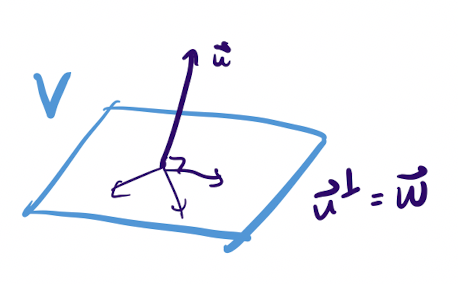
\includegraphics[width=5cm]{Lecture Files and Images/lec26-thm.png}
\end{center}

    \item \textbf{Case 2.} Otherwise, for every $v \in V,$ $\langle v, v \rangle = 0.$ This is a very strong constraint on the form, and in fact it forces $\langle v, w\rangle = 0$ for all $v, w,$ which forces \emph{any} basis to be an orthogonal basis. 
    To see this, consider the inner product on a sum of two vectors with itself:
    \begin{align*}
        0 &= \langle v + w, v + w \rangle \\
        &= \langle v, v \rangle + \langle w, w \rangle + \langle v, w \rangle + \langle w, v\rangle \\
        &= 2\langle v, w \rangle.
    \end{align*}
    When $F = \RR,$ we have $\langle v, w \rangle = 0,$ by the symmetry of the form. Otherwise, for $F = \CC,$ $\text{Re}(\langle v, w \rangle) = 0,$ and the same process can also be done for $v$ and $iw$ to show that $\langle v, w \rangle = 0.$ Then the inner product is 0 on any two vectors so every basis is orthogonal.
    %include this argument for \CC
\end{itemize}
\end{proof}
We can simplify the basis even further.
\begin{corollary}
In fact, $V$ has an orthogonal basis $\{v_1, \cdots, v_k\}$ where $\langle v_i, v_i\rangle = 1, -1,$ or 0. 
\end{corollary}
\begin{proof}
Take an orthogonal basis $\{x_1, \cdots, x_k\}$. Consider $\langle x_i, x_i \rangle$, which is a real number.
\begin{itemize}
    \item If the pairing is 0, then let $v_i = x_i.$
    \item Otherwise, we can normalize and take $v_i = \frac{1}{\sqrt{|\langle x_i, x_i \rangle|}}x_i;$ then $\langle v_i, v_i \rangle = \frac{\langle x_i, x_i \rangle}{|\langle x_i, x_i \rangle|},$ so it will be 1 or -1 depending on the sign of $\langle x_i, x_i \rangle.$
\end{itemize}
\end{proof}

In particular, if $\bform$ is non-degenerate, only $\pm 1$ occur. Also, if $\bform$ is positive definite, by definition, $\langle v, v \rangle > 0$ if $v \neq 0,$ so only $+1$s occur, so in that basis, the form looks just like the dot product or the standard Hermitian product.

The following claim will be shown in the upcoming problem set.

\begin{claim}[Sylvester's Law]
In fact, given $V$ and $\bform,$ the number of 1s, the number of -1s, and the number of 0s that occur in the diagonal form are determined by $V$ and $\bform,$ and not by the choice of orthogonal basis.\footnote{They are similar to eigenvalues in that while there are many choices of orthogonal basis, the \emph{number} of 1s, -1s, and 0s are not dependent on the particular basis.} This is called \emph{Sylvester's Law}, and the number of 1s, -1s, and 0s is called the \emph{signature} of the form. 
\end{claim}

For example, in the form used in special relativity, $\begin{pmatrix}-1 & & & \\ & 1 & & \\ & & 1 & \\ & & & 1\end{pmatrix}$, the signature is $(3, 1, 0).$

 %what does he say here LOL i missed it (below)
In matrix form, the corollary states that for a symmetric matrix $A \in \text{Mat}_{n \by n}(\RR)$, for which $A^T = A,$ there exists some matrix $P \in GL_n(\RR)$ such that $P^TAP$ is a diagonal matrix with all $1s, -1s$, or 0s on the diagonal:
\[
P^TAP = \begin{pmatrix} 1 & & & & & \\ & \ddots & & & &  \\ & & -1 & & &  \\ & & & \ddots & & \\ & & & & 0 & \\ & & & & & \ddots \end{pmatrix}.
\]

If $A$ is positive definite, which is when $x^T Ax > 0,$ there exists $P$ such that $P^TAP = I_n$ implies that $A = Q^TQ$, where $Q= P^{-1}$.

The statement is similar for complex matrices, where we replace the transposes with adjoints.
%add the statement for complex matrices
%ethany: i feel like this is unnecessary

%is the number of 1s and -1s set? ok sylvester's whatever

%what is the importance of the signature? does it tell you anything about the metric given by the inner product? 

\subsection{Projection Formula}

Consider a vector space $V$ and a form $\bform$, as well as a subspace $W$ for which $\bform|_W$ is non-degenerate. By Theorem \ref{non-degenerate stuff}, $V = W \oplus W^\perp$ such that $v = w + u.$ 

\begin{center}
    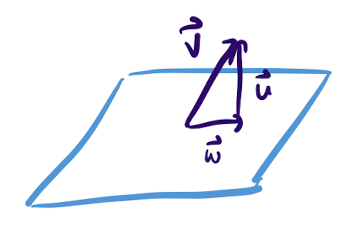
\includegraphics[width=5cm]{Lecture Files and Images/lec26-projection.png}
\end{center}

\begin{qq}
How can we compute $w$ and $u$?
\end{qq}
To do so, we use the orthogonal projection. We want a map
\begin{align*}
    \pi: V &\rto W \\
    v &\mto w,
\end{align*}
so that $v = \pi(v) \perp W.$\footnote{This is an extremely useful application of linear algebra! In geometric situations, the vector $w$ is the vector closest to $v$ of the vector in the plane, and perhaps these vectors are in a vector space of data points. Finding a formula for $w$ explicitly is called least-squares regression.}

Assuming there exists an orthogonal basis $\{w_1, \cdots, w_k\}$ for $W$, the formula for $\pi$ is simple.\footnote{Once we've developed the machinery for bilinear forms, these ideas become a lot simpler!} The vector can be written as 
\[
v = cw_1 + \cdots + cw_k + u,
\]
where $u \perp W.$ Then for all $i$, 
\[
\langle w_i, v \rangle = 0 + \cdots + 0 +c_i \langle w_i, w_i \rangle + 0 + \cdots + 0,
\]
so 
\[
c_i = \frac{\langle w_i, v\rangle}{\langle w_i, w_i \rangle}.
\]
It is not possible for $\langle w_i, w_i\rangle = 0,$ because the form would be degenerate. In fact, this formula is useful when $W = V$, because it provides a formula for the coordinates of some vector with respect to the orthogonal basis. 

\begin{example}
Let $V = \RR^3$ and $\bform$ be the dot product. Then let $W$ be the span of $\vec{w}_1 = (1, 1, 1)^T$ and $\vec{w}_1 = (1, 1, -2)^T.$ The pairings are $\langle w_1, w_1 \rangle = 3,$ $\langle w_2, w_2 \rangle = 6,$ $\langle w_1, v \rangle = 6,$ and $\langle w_2, v \rangle = -3.$ The projection of $(1, 2, 3)$ is then 
\[
\pi(v) = \frac{6}{3}w_1 -\frac{1}{2}w_2 = \begin{pmatrix}3/2 \\ 3/2 \\ 3\end{pmatrix}.
\]

To verify, $v - \pi(v) = (-1/2, 1/2, 0),$ which is orthogonal both to $w_1$ and $w_2.$
\end{example}

\newpage

\lhead{Lecture 27: Euclidean and Hermitian Spaces}
\setcounter{section}{26}
%MIT OpenCourseWare: https://ocw.mit.edu
%RES.18-011 Algebra I Student Notes, Fall 2021
%License: Creative Commons BY-NC-SA 
%For information about citing these materials or our Terms of Use, visit: https://ocw.mit.edu/terms.

\section{Euclidean and Hermitian Spaces}

\subsection{Review: Orthogonal Projection}
Last time, we ended by talking about orthogonal projections and splittings such that $V = W \oplus W^\perp$.
Specifically, suppose we have a vector space $V$ with a bilinear form $\bform$ as well as a subspace $W$ such that the restriction $\bform|_W$ is non-degenerate.
Then, given a orthogonal basis of $W = \spann \{ w_1, \ldots, w_k\}$, we were able to write a formula for the projection onto $W$:
\[\proj(v) = \frac{\langle w_1, v \rangle}{\langle w_1, w_1 \rangle } w_1 + \cdots + \frac{\langle w_k , v \rangle}{\langle w_k, w_k \rangle} w_k.\]
and we had that $v = \proj(v) + u$, where $\proj(v) \in W$ and $u \in W^\perp$. 

\subsection{Euclidean and Hermitian Spaces}
In order to evaluate the projection formula, we need an orthogonal basis of a subspace. How do we calculate this?

To start, we will be talking about Euclidean and Hermitian spaces. Recall that a pairing $\bform$ is positive definite if $\langle v, v \rangle >0$ for all $v \neq 0.$
\begin{definition}
A \textbf{Euclidean} space is a real vector space $V$ and a symmetric bilinear form $\bform$ such that $\bform$ is positive definite. Analogously, a \textbf{Hermitian} space is a complex vector space $V$ and a Hermitian form $\bform$ such that $\bform$ is positive definite.
\end{definition}

These spaces have the following nice property.
\begin{theorem}
If $V$ is Euclidean or Hermitian, then there exists an orthonormal basis $\{v_1, \cdots, v_n \}$ for $V$ such that $\langle v_i, v_j \rangle = 0$ and $\langle v_i, v_i \rangle = 1$. In particular, the pairing $\bform$ looks like the dot product or the standard Hermitian product in this basis. 
\end{theorem} 
\begin{proof}
    From last time, we saw that for any pairing, there exists an orthogonal basis where all of the self-pairings were either 1, 0, or $-1.$
    By definition, all of the self-pairings must be 1 when the form is positive definite.
\end{proof}
Furthermore, we no longer have the case where a form can be degenerate on a subspace. 
\begin{claim}
    For any $W \subseteq V$ and $\bform|_W,$ the restriction $\bform|_W$ is \emph{always} nondegenerate. 
\end{claim}
\begin{proof}
For each $w \in W,$ we need to find a $w' \in W$ such that $\langle w, w'\rangle \neq 0$. By the positive definiteness of the pairing, we can just take $w' = w.$ 
\end{proof}
This means that we can inherit all the properties that we showed last time about non-degenerate subspaces. 
In particular, we can always perform the orthogonal projection on any subspace of a Euclidean/Hermitian space.

\subsection{Gram-Schmidt Algorithm}
As an application, we have the \textbf{Gram-Schmidt algorithm} for finding an orthonormal basis. 
Take a Euclidean or Hermitian vector space $V$ and any basis $\{v_1, \cdots, v_n\}$ a basis for $V.$ In order to build an orthonormal basis $\{u_1, \cdots, u_n\},$ we inductively build $\{u_i\}$ such that $\spann\{u_1\} = \spann\{v_1\},$ $\spann\{u_1, u_2\} = \spann\{v_1, v_2\},$ and so on. Let $V_k = \spann\{v_1, \cdots, v_k\}.$

\begin{itemize}
    \item \textbf{Step 0.} Our first vector must just be a scaled version of $v_1$. We have to scale it such that $\langle u_1, u_1 \rangle = 1$. 
    Let \[u_1 \coloneqq \frac{1}{\sqrt{\langle v_1, v_1 \rangle}}v_1.\] Then $\{u_1\}$ is a basis for $V_1$ and $\langle u_1, u_1 \rangle = 1.$
    
    \item \textbf{Step 1.} Set \[x_2 = \proj_{V_1}v_2,\] which is the projection of $v_2$ onto $V_1,$ and let \[y_2 = v_2 - x_2,\] which is the orthogonal portion of the vector $v_2.$ Then, let 
    \[
    u_2 = \frac{1}{\sqrt{\langle y_2, y_2\rangle}} y_2
    \]
    be the result of normalizing $y_2$. Then $\langle u_1, u_2 \rangle = 0,$ since the portion of $v_2$ spanned by $u_1 $ has been subtracted off, and $\langle u_2, u_2 \rangle = 1.$ Thus $\{u_1, u_2\}$ is an orthonormal basis of $V_2.$
    
    \item \textbf{Step $k.$} Assume that $\{u_1, \cdots, u_k\}$ is a basis for $V_k.$ Then, let 
    \[
    x_{k + 1} = \proj_{V_k}(v_{k + 1})y_k,
    \]
    the projection onto $V_k,$ and let
    \[
    y_{k + 1} = v_{k + 1} - x_{k + 1},
    \]
    the orthogonal portion of $v_{k +1}.$ Then let 
    \[
    u_{k + 1} = \frac{1}{\langle y_{k + 1}, y_{k + 1} \rangle}.
    \]
    By induction, $\{u_1, \ldots, u_{k+1} \}$ is an orthonormal basis for $V_{k+1}$.
    
    
    
\end{itemize}
At every step, the projection formula is used, until a basis is found. Note that whenever we are calculating the projection, we conveniently have an orthogonal (even more, orthonormal) basis of the previous subspace to use the projection formula.
Specifically, on step $k$ the projection formula simplifies to: \[ \proj_{v_k} (v_{k+1}) = \langle u_1, v_{k+1} \rangle u_1 + \cdots + \langle u_k, v_{k+1} \rangle u_k.\]

We can interpret the algorithm in matrix form as well. 
Take $M \in GL_n(\RR).$ The columns of $M$, $\{v_1, \cdots, v_n\}$, are a basis for $\RR^n.$ 
The Gram-Schmidt algorithm says that we can take this basis and turn it into an orthonormal basis:
\begin{align*}
    u_1 &= a_{11}v_1 \\
    u_2 &= a_{12}v_1 + a_{22}v_2 \\
    u_3 &= a_{13}v_1 + a_{23}v_2 + a_{33}v_3,
\end{align*}
and so on, where $\{u_1, \cdots, u_n\}$ is an orthonormal basis of $\RR^n$.
The upshot is that there exists an upper triangular matrix $A$ and an orthogonal matrix $B$ such that \[M = AB.\] $A$ is the matrix derived from putting $u_i$ as columns, and $B$ is the inverse of the matrix derived from the $a_{ij}$ values.  
\begin{question}
    What sense of orthogonal are we using in the algorithm?
\end{question}
\begin{ans}
    This algorithm refers to orthogonal bases with respect to the standard dot product. 
    One could consider more general kinds of symmetric bilinear forms, and what results are different kinds of groups. 
    We will look at this later. 
    
    For Euclidean spaces, we can consider all pairings as the dot product, so orthogonality always is just the normal definition.
    When the pairing is not positive definite, then we start getting weirder things.
\end{ans}
\subsection{Complex Linear Operators}
Now, we want to focus on linear operators in a Hermitian space $(V, \bform)$. Consider a linear operator 
\[
T: V \rto V.
\]
%Then the Hermitian property of the space provides another linear operator. 
We can the define the analogue of the adjoint operation on matrices.
\begin{definition}
Pick an orthonormal basis $\{u_1, \cdots, u_n\}$ of our Hermitian space. By doing so, we can map our vector space into coordinate vectors. We have the correspondence $V \rightsquigarrow \CC^n$, and the form $\bform$ maps to the standard Hermitian product. Then, $T \rightsquigarrow M \in \text{Mat}_{n \by n}(\CC).$ Then let the \textbf{adjoint} $T^*$ be the linear operator
\[
T^*: V \rto V
\]
such that, with respect to the basis $\{u_1, \cdots, u_n \}$, $T^*$ is the matrix $M^* = \overline{M^T}$. 
\end{definition}

The following claim gives the key property of the adjoint linear operator and another way to characterize the adjoint operator.

\begin{claim}
For $v, w \in V,$
\[
\langle Tv, w \rangle = \langle v, T^*w\rangle.
\]
This property means that $T^*$ is uniquely determined, by putting $v = u_i$ and $w = u_j.$
\end{claim}

\begin{proof}
Using the correspondence given by taking a basis, 
\begin{align*}
    v &\rightsquigarrow x \in \CC^n \\
    w &\rightsquigarrow y \in \CC^n \\
    Tv &\rightsquigarrow Mx \in \CC^n.
\end{align*}
Then, 
\[
\langle Tv, w \rangle = (Mx)^*y = x^*M^*y = x^*(M^*y) = \langle v, T^*w\rangle.
\]
\end{proof}

This also means that $T^*$ is independent of the choice of a basis.

%Our earlier work can be carried into the world of Hermitian spaces. A Hermitian matrix was defined to be a matrix such that $A^* = A$. %watch again
Just as we defined adjoint for both linear operators and matrices, we can do the same for the definition of Hermitian.
\begin{definition}
A linear operator $T: V \rto V$ is a \textbf{Hermitian operator} if $T^* = T,$ which is equivalent to $\langle Tv, w \rangle = \langle v, Tw \rangle.$ %check if it's Tw or T^*w
\end{definition}

Also, a unitary matrix is a matrix such that $U^*U = I_n$ and $U^* = U^{-1}.$ The following definition is analogous.
\begin{definition}
A linear operator $T: V \rto V$ is a \textbf{unitary} operator if $T^*T = \text{Id}$, or equivalently if $\langle Tv, Tw \rangle = \langle v, w \rangle$ for all $v, w \in V.$
\end{definition}

The following definition is harder to motivate, but encapsulates the previous two. 
\begin{definition}
A linear operator $T:V \rto V$ is \textbf{normal} if $T T^* = T^*T$, which is equivalent to \[\langle v, T^*Tw \rangle = \boxed{\langle Tv, Tw \rangle = \langle T^*v, T^*w \rangle} = \langle v, TT^*w \rangle.\]
\end{definition}

The set of unitary matrices and the set of Hermitian matrices are both subsets of the set of normal matrices. However, there are normal matrices that are neither Hermitian nor unitary. For example, $A = \begin{pmatrix}1 & 1 & 0 \\ 0 & 1 & 1 \\ 1 & 0 & 1 \end{pmatrix}$ is \emph{normal} but neither Hermitian nor unitary. 

Next class, we will discuss the \emph{Spectral Theorem}, which is the main important property of normal matrices.
\begin{theorem}[Spectral Theorem]
For a Hermitian space $V,$ and a normal linear operator $T: V \rto V$, $V$ has an orthonormal basis $\{u_1, \cdots, u_n\}$ where each $u_i$ is an eigenvector of $T.$
\end{theorem}
In other words, we both diagonalize $T$ as well as find an orthonormal basis for $V$. 
We don't need to mess around with Jordan forms. 

The matrix version states that for a normal matrix $M \in \text{Mat}_{n \by n}(\CC)$,\footnote{$M^*M = MM^*$} it is possible to find a unitary matrix $P$\footnote{$P^*P = I$} such that \[P^*MP = P^{-1}MP = \begin{pmatrix} \lambda_1 & & \\
& \ddots & \\ & & \lambda_n\end{pmatrix}.\] The columns of $P$ form our eigenbasis. 

What about Euclidean spaces? In full generality, this theorem is false. However, for a Euclidean space $V$ and a \emph{symmetric} linear operator $T: V \rto V$, $T$ does have an orthonormal eigenbasis. Generalizing from symmetric to orthogonal, which is the analogous version of unitary, or some condition similar to ``normal," does not work. For example, we saw that it is not true for orthogonal matrices, as rotation matrices in the plane do not have any eigenvectors. 

\newpage

\lhead{Lecture 28: The Spectral Theorem}
\setcounter{section}{27}
%MIT OpenCourseWare: https://ocw.mit.edu
%RES.18-011 Algebra I Student Notes, Fall 2021
%License: Creative Commons BY-NC-SA 
%For information about citing these materials or our Terms of Use, visit: https://ocw.mit.edu/terms.

\section{The Spectral Theorem}

\subsection{Review: Hermitian Spaces}
Last time, we discussed Hermitian spaces which were just complex vector spaces with a positive definite Hermitian form.  
Given a linear operator $T$, we defined the adjoint $T^*$, which had the property that \[\langle v, T^* w \rangle = \langle Tv, w\rangle. \]
We called a linear operator $T$ normal if $TT^* = T^* T$. 
We then were able to state the Spectral Theorem.

\subsection{The Spectral Theorem}

The Spectral Theorem demonstrates the special properties of normal and real symmetric matrices.
\begin{theorem}
Given a Hermitian space $V$, for any normal linear operator $T$, there exists an orthonormal eigenbasis of $V$: $\{u_1, \cdots, u_n\}.$ In matrix form, for any normal matrix $M \in GL_n(\CC),$ there exists a unitary matrix $P$ such that $P^{-1} M P$ is diagonal.


The real version states that for a Euclidean vector space $V$ and a \emph{symmetric} linear operator $T$, there exists an orthonormal eigenbasis; equivalently, for any symmetric matrix $M \in GL_n(\RR)$, there exists an orthogonal matrix $P$ such that $P^{-1}MP$ is diagonal. All eigenvalues of real symmetric matrices are real.
\end{theorem}

\begin{example}
    Say we take the symmetric matrix $M = \begin{bmatrix} 3 & -1 \\ -1 & 3 \end{bmatrix}$.
    One eigenvector is $\frac{1}{\sqrt{2}}\begin{bmatrix}1 \\ 1 \end{bmatrix}$ with eigenvalue $\lambda_1 = 2$. 
    The other eigenvector should be orthogonal, so it is $\frac{1}{\sqrt{2}}\begin{bmatrix}1 \\ -1 \end{bmatrix}$ with eigenvalue $\lambda_2 = 4$.

    In 2 dimensions, the fact that our change of basis is coming from an orthogonal basis tells us that the change in coordinates is just a rotation. 
    This rotation makes the operator diagonalizable. 
\end{example}
This is called the Spectral Theorem because the eigenvalues are often referred to as the spectrum of a matrix. 
Any theorem that talks about diagonalizing operators is often called a spectral theorem. 

Now we will state some lemmas in order to prove the Spectral Theorem.
\begin{lemma}[Lemma 1]
First, for a linear operator $T: V \rto V$ where $V$ is Hermitian, and a subspace $W \subset V$ such that $T(W) \subset W,$ then $T^*(W^\perp) \subset W^{\perp}.$
\end{lemma}
\begin{proof}
Take some $u \in W^\perp.$ For any $w \in W,$ then 
\[
\langle w, T^*u \rangle = \langle Tw, u\rangle = 0,
\]
by the definition of the adjoint linear operator, so $T^*u \in W^\perp.$
\end{proof}

\begin{lemma}[Lemma 2]
If $Tv = \lambda v,$ then $T^*v = \overline{\lambda}v.$
This just means that $T$ and $T^*$ have the same eigenvectors, and eigenvalues related by complex conjugation.
\end{lemma}
\begin{proof}
We can first consider a special case.
\begin{itemize}
    \item \textbf{Special Case:} $\lambda = 0.$ We want to show that $Tv=0$ implies that $T^*v = 0$.
    \[
    \langle T^*v, T^*v \rangle = \langle Tv, Tv \rangle = 0
    \]
    by normality (this was a property shown last time). 
    Since $T$ is positive definite, this implies that $T^*v = 0.$  
    This also implies that if a vector $v \in \Ker T$, then $v \in \Ker T^*$ as well.
    \item \textbf{General Case:} $\lambda \in \CC.$ We want to show that $Tv = \lambda v$ implies that $T^*v = \lambda v$. In this case, create a new linear operator $S = T - \lambda I.$ Then, $Sv = 0.$ Also, the adjoint is $S^* = T^* - \overline{\lambda}I$ and $SS^* = S^*S,$ since $TT^* = T^*T.$ %By the earlier case, $S^*v = 0$ implies that $T^*v = \overline{\lambda}v.$
    By the first case, since $v\in \Ker S$, we also have that $v \in \Ker S^*$ so $T^* = \overline{\lambda} v$ as needed.
\end{itemize}
\end{proof}

\begin{proof}[Proof of the Spectral Theorem]
Now we can prove the Spectral Theorem by induction on the dimension of $V.$ The general process will be breaking $V$ up into a direct sum and finding orthonormal eigenbases over each part.
Since the field is $F = \CC,$ it is always possible to find an eigenvector $w \in V$ such that $Tw = \lambda w.$ By normalizing $w,$ assume that $\langle w, w \rangle = 1.$ Then, let $W = \spann(w);$ then $V = W \oplus W^\perp$ since all subspaces of Hermitian spaces are non-degnerate. In addition, since $w$ is an eigenvector, $TW \subset W.$ 

If we can show that $TW^\perp$ preserves $W^\perp$, then we can induct.
By Lemma 2, $w$ is also an eigenvector of $T^*$, so $T^*(W) \subset W,$ and by Lemma 1, $(T^*)^*(W^\perp) = T(W^\perp) \subset W^\perp.$ Then $V = W \oplus W^\perp,$ and $T$ maps each part of the splitting to itself, so by induction there exists $u_2, \cdots, u_n$ an orthonormal eigenvasis for $W^\perp,$ and $\{w, u_2, \cdots, u_n\}$ is an orthonormal eigenbasis for $V.$ 
\end{proof}

\begin{question}
Why is the equivalent of the theorem not true over the real numbers? 
\end{question}
\begin{ans}
Most of this argument works, except in the very first step, where we found an eigenvector and eigenvalue. We cannot guarantee this will happen with normal linear operators over the real numbers. However, as we found last week, for symmetric (and Hermitian) matrices, the eigenvalues are all real, and in particular it is always possible to find one eigenvector $w \in V$ with real eigenvalue to allow the induction to occur.
\end{ans}

%ADD proof in euclidean case from davesh notes

As an application, suppose we have a quadratic function $f(x, y) = ax^2 + bxy + cy^2.$ Let this function be represented by a matrix 
$
\begin{pmatrix}
a & b/2 \\
b/2 & c
\end{pmatrix}$; then \[
f(x, y) = (x, y) M \begin{pmatrix}
x \\ y
\end{pmatrix} = \langle v, Tv \rangle
\]
for a linear operator $T$ given by $M.$ By the Spectral Theorem, there exists an orthogonal change of coordinates $P^TMP = \begin{pmatrix}
\lambda_1 & 0 \\ 0 & \lambda_2
\end{pmatrix},$ where $P$ is an orthogonal matrix. It takes $\begin{pmatrix}
x \\ y
\end{pmatrix} = P\begin{pmatrix}
x' \\ y'
\end{pmatrix}$. Then 
\[
f(x, y) = (x, y) M \begin{pmatrix}
x \\ y
\end{pmatrix} = (x', y') \begin{pmatrix}
\lambda_1 & \\ & \lambda_2
\end{pmatrix}\begin{pmatrix}
x'\\ y'
\end{pmatrix} = \lambda_1(x')^2 + \lambda_2(y')^2.
\]

\begin{example}

If $f(x, y) = 3x^2 - 2xy + 3y^2,$ the matrix would be $M = \begin{pmatrix}
3 & -1 \\ -1 & 3
\end{pmatrix}$. Then 
\[
3x^2 - 2xy + 3y^2 = 2(x')^2 + 4(y')^2,
\]
for some change of coordinates taking $x$ and $y$ to  $x'$ and $y',$ since we saw earlier that the eigenvalues were $2$ and $4.$ 

\end{example}

In $n$ variables, let $f(x_1, \cdots, x_n) = a_{11} x_1^2 + \cdots + a_{nn}x_n^2 + \sum_{i < j} 2a_{ij}x_ix_j$ be represented by the matrix $M = (a_{ij}) = \begin{pmatrix}
a_{11} & \cdots & a_{ij} & \\
\vdots & \ddots & & \\
a_{ji} & & \ddots& \\
& & & a_{nn}
\end{pmatrix}.$ %fix this matrix

Applying the spectral theorem gives $P$ and $\lambda_i$, where $P$ is a change of coordinates taking $\begin{pmatrix}
x_1 \\ \vdots \\ x_n
\end{pmatrix} = P\begin{pmatrix}
x'_1 \\ \vdots \\ x'_n
\end{pmatrix}.$ In this new coordinate system, 
\[
f(x_1, \cdots, x_n) = \lambda_1(x'_1)^2 + \cdots + \lambda_n(x'_n)^2.
\]

In two and three dimensions, this has a geometric interpretation. Consider a curve in $\RR^2$ with an equation of the form
\[
ax^2 + bxy + cy^2 + dx + ey + f = 0.
\]

There are several options; the first three are called conics, and the rest are degenerate conics of some form.
\begin{itemize}
    \item \textbf{Ellipse.} $ax^2 + by^2 = 1$
    \item \textbf{Hyperbola.} $ax^2 - by^2 = 1$
    \item \textbf{Parabola.} $ax^2 - y = 0$
    \item \textbf{Two crossing lines.} $(a_1x + b_1y)(a_2x + b_2y) = 0$
    \item \textbf{Two parallel lines.} $x^2 = a, a > 0$
    \item \textbf{One line.} $x^2 = 0$ 
    \item \textbf{One point.} $x^2 + y^2 = 0$
    \item \textbf{The empty set $\varnothing$.} $x^2 + y^2 = -1$
\end{itemize}

\begin{theorem}
After an isometry, all curves of the form $ax^2 + bxy + cy^2 + dx + ey + f = 0$ look like one of these options. 
\end{theorem}
\begin{proof}
The curve be rewritten as $\vvv^TA\vvv + B\vvv + f = 0.$ After an orthogonal change of basis, we can assume that $A = \begin{pmatrix}
\lambda_1 & 0 \\ 0 & \lambda_2.
\end{pmatrix}$
Then $\lambda_1x^2 + \lambda_2y^2 + b_1x + b_2y + f = 0.$ 
\begin{itemize}
    \item \textbf{Nonzero eigenvalues.} If $\lambda_1, \lambda_2 \neq 0,$ then we can complete the square, taking $x \rightsquigarrow x + \frac{b_1}{2\lambda_1}$ and $y \rightsquigarrow y + \frac{b_2}{2\lambda_2}$. Then 
    \[
    \lambda_1x^2 + \lambda_2y^2 = c.
    \]
    If $c = 0,$ it is a single point or two intersecting lines, and if $c \neq 0,$ it is an ellipse or a hyperbola. 
    
    \item \textbf{Zero eigenvalues.} The other cases. 
\end{itemize}
The details of this aren't that important, and we glossed over much of it at the end. 
The main idea to take away is just the power of the Spectral Theorem to take a complicated quadratic form and simplify into something more readily analyzed. 
\end{proof}

One idea where the Spectral Theorem is at play is in multivariable calculus with the second derivative test.
Hidden behind the test is that we have a symmetric matrix and we are trying to figure out what the signs of the eigenvalues are, as that will tell us whether our critical point is a minimum, maximum, or saddle point.

\newpage

\lhead{Lecture 29: Geometry of $SU_2$}
%MIT OpenCourseWare: https://ocw.mit.edu
%RES.18-011 Algebra I Student Notes, Fall 2021
%License: Creative Commons BY-NC-SA 
%For information about citing these materials or our Terms of Use, visit: https://ocw.mit.edu/terms.

\section{Linear Groups}

Today we'll study \textbf{linear groups} -- subgroups of matrices which satisfy conditions about preserving properties that come from linear algebra. We've seen a couple of these already. We can start off with the group $GL_n(\mathbb{R})$ of all invertible $n \times n$ matrices, and consider a few subgroups that we've seen:
\begin{center}
    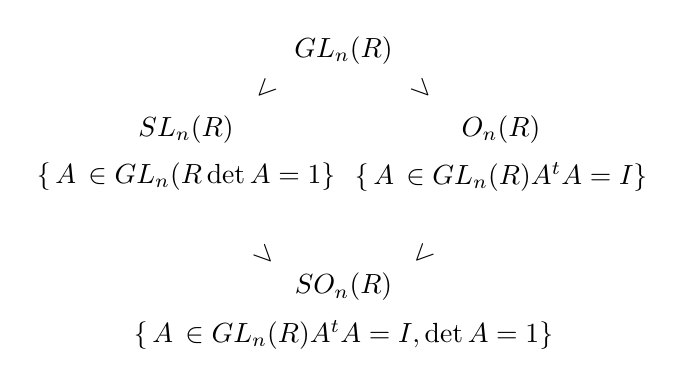
\begin{tikzpicture}[scale=2]
        \node (GLR) at (0, 1.5) {$GL_n(\mathbb{R})$};
        \node [label=below:{$\left\{\begin{matrix} A \in GL_n(\mathbb{R} \\ \det A = 1 \end{matrix}\right\}$}] (SLR) at (-1, 1) {$SL_n(\mathbb{R})$};
        \node [label=below:{$\left\{\begin{matrix} A \in GL_n(\mathbb{R}) \\  A^tA = I \end{matrix}\right\}$}] (OR) at (1, 1) {$O_n(\mathbb{R})$};
        \node [label=below:{$\left\{\begin{matrix}A \in GL_n(\mathbb{R}) \\ A^tA = I, \det A = 1 \end{matrix}\right\}$}] (SOR) at (0, 0) {$SO_n(\mathbb{R})$};
        \node [rotate=45] at (-0.5, 1.25) {$<$};
        \node [rotate=135] at (0.5, 1.25) {$<$};
        \node [rotate=135] at (-0.5, 0.2) {$<$};
        \node [rotate=45] at (0.5, 0.2) {$<$};
    \end{tikzpicture}
\end{center}
These subgroups all preserve some interesting property:
\begin{itemize}
    \item $SL_n(\RR) \leq GL_n(\RR)$ consists of the matrices with determinant 1, which preserve volume.
    \item $O_n(\RR) \leq GL_n(\RR)$ consists of the orthogonal matrices, which preserve the dot product (or equivalently, which preserve length) -- meaning that $\langle Av, Aw\rangle = \langle v, w\rangle$ for any two vectors $v$, $w$ (where the pairing denotes the dot product). 
    \item $SO_n(\RR)$ is the intersection of $SL_n(\RR)$ and $O_n(\RR)$. 
\end{itemize}

We can do the same thing for matrices with complex values:
\begin{center}
    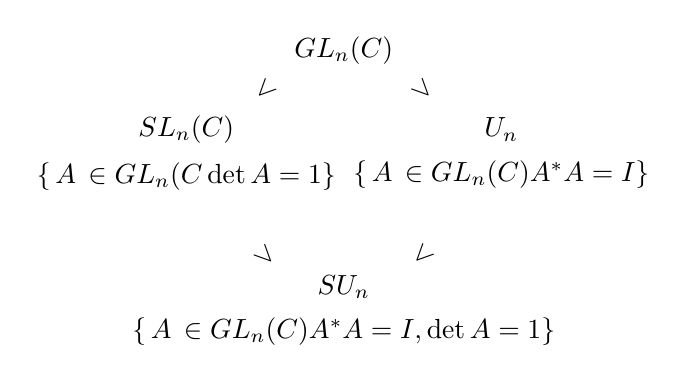
\begin{tikzpicture}[scale=2]
        \node (GLR) at (0, 1.5) {$GL_n(\mathbb{C})$};
        \node [label=below:{$\left\{\begin{matrix} A \in GL_n(\mathbb{C} \\ \det A = 1 \end{matrix}\right\}$}] (SLC) at (-1, 1) {$SL_n(\mathbb{C})$};
        \node [label=below:{$\left\{\begin{matrix} A \in GL_n(\mathbb{C}) \\  A^*A = I \end{matrix}\right\}$}] (U) at (1, 1) {$U_n$};
        \node [label=below:{$\left\{\begin{matrix}A \in GL_n(\mathbb{C}) \\ A^*A = I, \det A = 1 \end{matrix}\right\}$}] (SU) at (0, 0) {$SU_n$};
        \node [rotate=45] at (-0.5, 1.25) {$<$};
        \node [rotate=135] at (0.5, 1.25) {$<$};
        \node [rotate=135] at (-0.5, 0.2) {$<$};
        \node [rotate=45] at (0.5, 0.2) {$<$};
    \end{tikzpicture}
\end{center}
These subgroups still preserve some linear algebraic property:
\begin{itemize}
    \item $SL_n(\CC) \leq GL_n(\CC)$ is still the group of matrices with determinant $1$, the same as in the real case. 
    \item $U_n(\CC) \leq GL_n(\CC)$ is the group of unitary matrices, which preserve the standard Hermitian form -- so $\langle Av, Aw\rangle = \langle v, w\rangle$ where the pairing is now the standard Hermitian form (instead of the dot product, as in $O_n(\mathbb{R})$ for the real numbers).  
    \item $SU_n(\CC)$ is the intersection of $SL_n(\CC)$ and $U_n(\CC)$, the group of unitary matrices with determinant $1$.
\end{itemize}
We could also look at groups of matrices that preserve other bilinear forms, not just the dot product. For example, we could define the bilinear form $I_{p,q}$ corresponding to the matrix $\begin{bmatrix} I_p & \\ & -I_q \end{bmatrix}$. 
Then we could study the matrices preserving this bilinear form, meaning the set $\{A \mid A^t I_{p,q} A = I_{p, q}\}$, which is an interesting subgroup of $GL_n(\mathbb{R})$. 

\subsection{Geometry of groups}

All these matrices are over $\RR$ or $\CC$. What's special about the real or complex numbers, as opposed to something like a finite field, is that we have a notion of \emph{distance}. More explicitly, we have $GL_n(\mathbb{R}) \subset \mathbb{R}^{n^2}$ (where we just write down the coordinates), so $GL_n(\mathbb{R})$ inherits a \textbf{metric} -- we can discuss whether two elements are close together or far apart. The same works for $GL_n(\mathbb{C}) \subset \mathbb{R}^{2n^2}$ (since we can think of a complex number as a pair of real numbers). 

The actual metric itself won't be that important; what will be important is the idea of a \textbf{topology} on this set -- we have a sense of two elements being close together or far apart, which we didn't have when we studied finite or discrete groups. With finite or discrete groups, we can't really talk about a sequence of elements getting closer and closer to another, but with these groups we can. The group structure and topology interact with each other in extremely interesting ways -- these groups are called \textbf{Lie groups}, and the study of such groups ends up being a really rich vein of mathematics.

Today we'll see a flavor of how we can take a group and look at it not just as a collection of things, but also as having some sort of geometry. 

There are some questions we can ask: groups come with multiplication law, $G \times G \rto G$. It turns out that for all the matrix groups considered above, the multiplication law is continuous (if you perturb two elements a bit, this only perturbs their product a bit as well). The inverse map $g \mapsto g^{-1}$ is also continuous. Similarly, we can look at \emph{continuous} homomorphisms. 

We've seen a few simpler examples of groups with a shape (not necessarily matrix groups) -- for example, $(\RR, +)$ is just the real line:
\begin{center}
    \begin{asy}
    unitsize(3cm);
    draw((0, 0)--(2, 0), Arrows);
    \end{asy}
\end{center}

\begin{example}
How can we draw the group of $2$-dimensional rotations \[SO_2 = \{\rho_\theta \mid 0 \leq \theta < 2\pi\}?\] 
\end{example}

\begin{proof}
    On a homework problem, we showed that $SO_2 \cong \mathbb{R}/2\pi \mathbb{Z}$. So we can draw $SO_2$ as a circle, where the angle represents the angle of rotation:
    \begin{center}
        \begin{asy}
            import geometry;
            unitsize(2cm);
            draw(circle((0, 0), 1));
            draw((1, 0)--(0, 0)--dir(40));
            markangle("$\theta$", radius=10, (1, 0), (0, 0), dir(40));
        \end{asy}
    \end{center}
    We have a homomorphism $\mathbb{R} \to SO_2$ where we send $\theta \mapsto \rho_\theta$. Geometrically, this corresponds to wrapping the line around the circle infinitely many times. 
\end{proof}

Similarly, we can consider $O_2$ -- we saw that $SO_2$ has two cosets, itself and the set of reflections. So we can think of $O_2$ as two circles (with one circle representing each). 

\begin{note}
We haven't really defined terms like continuous, metric, or topology. But we won't be that formal here; instead, the main goal is to try to visualize our groups in terms of these pictures. 
\end{note}

\subsection{Geometry of \texorpdfstring{$SU_2$}{SU2}}

All the groups whose geometry we've looked at so far are one-dimensional. Now we'll look at a higher-dimensional group, the \textbf{special unitary group} \[SU_2 = \{ A \in GL_2 (\CC) \mid \det A = 1, A^* = A^{-1} \}.\] We'll try to figure out what the points in this set look like, as a geometric shape. 

\subsubsection{Quaternions}

First we'll analyze what matrices are in $SU_2$. Consider a matrix $A = \begin{bmatrix} \alpha & \beta \\ \gamma & \delta \end{bmatrix}$. Then we have \[A^{-1} = \frac{1}{\det A} \begin{bmatrix} \delta & -\beta \\ -\gamma & \alpha \end{bmatrix} = \begin{bmatrix} \delta & -\beta \\ -\gamma & \alpha \end{bmatrix}\] (since the determinant is $1$), and \[A^* = \begin{bmatrix} \overline{\alpha} & \overline{\gamma} \\ \overline{\beta} & \overline{\gamma} \end{bmatrix}.\] These must be equal, so we must have $\delta = \overline{\alpha} $ and $\beta = - \overline{\gamma}$. 
Thus we must have \[A = \begin{bmatrix}\alpha & \beta \\ -\overline{\beta} & \overline{\alpha} \end{bmatrix}.\] Finally, the condition that $\det A = 1$ means that $|\alpha|^2 + |\beta|^2 = 1$. 

We can write any matrix $A$ as a linear combination of other matrices, by splitting up the real and imaginary parts of $\alpha$ and $\beta$. Suppose $\alpha = x_0 + i x_1$ and $\beta = x_2 + i x_3$ where $x_0, x_1, x_2, x_3 \in \RR$. Then we have
\[ A = x_0 \begin{bmatrix} 1 & 0 \\ 0 & 1\end{bmatrix} + x_1 \begin{bmatrix} i & 0 \\ 0 & -i \end{bmatrix} + x_2 \begin{bmatrix} 0 & 1 \\ -1 & 0 \end{bmatrix} + x_3 \begin{bmatrix} 0 & i \\ i & 0 \end{bmatrix} .\] 

We'll introduce some notation for these matrices. The first is just the other identity; meanwhile we define
\[ \mathbf{i} = \begin{bmatrix} i & 0 \\ 0 & -i \end{bmatrix}, \, \mathbf{j} = \begin{bmatrix}0 & 1 \\ -1 & 0 \end{bmatrix}, \, \mathbf{k} = \begin{bmatrix} 0 & i \\ i & 0 \end{bmatrix} . \]


We will also define a four-dimensional real vector space consisting of all matrices of the above form (which are linear combinations of $I$, $\mathbf{i}$, $\mathbf{j}$, and $\mathbf{k}$:
\[\mathbb{H} = \RR^4 = \{x_0 I + x_1 \mathbf{i} +x_2 \mathbf{j} + x_3 \mathbf{k} \mid x_0, x_1, x_2, x_3 \in \RR\} \subset \operatorname{Mat}_{2\times 2} (\CC).\] 
This space is closed under multiplication, since we can use the relations $\mathbf{i}^2 = \mathbf{j} = \mathbf{k}^2 = -I$, $\mathbf{i} \mathbf{j} = \mathbf{k}$, $\mathbf{j} \mathbf{i} = - \mathbf{k}$, and so on. So if we multiply any two elements of $\mathbb{H}$, we get another element of $\mathbb{H}$. 

The set $\mathbb{H}$ is called the set of \textbf{quaternions}. They're like a four-dimensional version of the complex numbers (instead of adding one square root of $-1$, we now have three). But unlike the complex numbers, multiplication isn't commutative -- so it's kind of like the field of complex numbers, but it's not a field because of the lack of commutativity. (We can still divide by nonzero elements, but we have to be careful about the order.)

But the main thing we'll use here is that it's a four-dimensional real vector space -- we've figured out how to write elements in terms of coordinates. Then $SU_2 \subset \mathbb{H}$ are exactly the quaternions such that $x_0^2 + x_1^2 + x_2^2 + x_3^2 = 1$ (since this is equivalent to the determinant condition). So $SU_2$ sits inside $\mathbb{R}^4$, and consists of all vectors with length $1$ -- this means its shape is a $3$-dimensional sphere $S^3$. 

\begin{question}
    Why is it called a 3-dimensional sphere if there are four dimensions?
\end{question}

\begin{ans}
    There's four dimensions, but we're imposing an additional condition. A sphere only consists of the boundary, not the interior (a sphere with its interior is called a \emph{ball}). So although it lives in four dimensions, it's a three-dimensional surface (because we have one constraint). Similarly, a normal sphere in $\RR^3$ is called a $2$-sphere, since its surface is two-dimensional. 
\end{ans}

\subsubsection{Geometry of the Sphere}

The $3$-sphere is very hard to picture, so let's start by drawing the 2-sphere \[S^2 = \{(x_0, x_1, x_2) :  x_0^2 + x_1^2 +x_2^2 = 0 \} \subset \RR^3.\] 

As coordinates, $S^2$ is the set of solutions to $x_0^2 + x_1^2 + x_2^2 = 1$. There are many ways of representing its coordinates, but one commonly used one is spherical coordinates, which we can think of in terms of latitude and longitude. 

The latitude lines come from taking a horizontal slice of the sphere -- formally, $\operatorname{Lat}_c = \{x_0 = c\} \cap S^2$. 

\begin{center}
        \begin{asy}
            unitsize(2.5cm);
            draw(circle((0, 0), 1));
            real latc(real a, real b) {
                return sqrt((1 - a^2)*(a^2 - b^2)/a^2);
            }
            path lat2(real a, real b) {
                return shift((0, latc(a, b)))*scale(a, b)*arc((0, 0), 1, 0, 180);
            }
            path lat1(real a, real b) {
                return shift((0, latc(a, b)))*scale(a, b)*arc((0, 0), 1, 180, 360);
            }
            draw(lat1(1, 0.2), gray);
            draw(lat2(1, 0.2), gray+dashed);
            real aq = 0.8;
            real bq = aq/5;
            draw(lat1(aq, bq), heavycyan);
            draw(lat2(aq, bq), heavycyan+dashed);
            draw(rotate(180)*lat2(aq, bq), heavycyan);
            draw(rotate(180)*lat1(aq, bq), heavycyan+dashed);
        \end{asy}
    \end{center}
The latitude lines start off as a point at the north pole $\operatorname{Lat}_1$, and then as we go downwards, they get bigger and bigger until the equator $\mathbb{E} = \operatorname{Lat}_0$, and then get smaller again until the south pole. 

Meanwhile, in the other direction, we have longitude lines, which are circles of radius $1$ that intersect the north and south pole. 
\begin{center}
        \begin{asy}
            unitsize(2.5cm);
            draw(circle((0, 0), 1));
            real latc(real a, real b) {
                return sqrt((1 - a^2)*(a^2 - b^2)/a^2);
            }
            path lat2(real a, real b) {
                return shift((0, latc(a, b)))*scale(a, b)*arc((0, 0), 1, 0, 180);
            }
            path lat1(real a, real b) {
                return shift((0, latc(a, b)))*scale(a, b)*arc((0, 0), 1, 180, 360);
            }
            draw(lat1(1, 0.2), gray);
            draw(lat2(1, 0.2), gray+dashed);
            real aq = 0.8;
            real bq = aq/5;
            draw(lat1(aq, bq), heavycyan);
            draw(lat2(aq, bq), heavycyan+dashed);
            draw(rotate(180)*lat2(aq, bq), heavycyan);
            draw(rotate(180)*lat1(aq, bq), heavycyan+dashed);
            real vr = 0.4;
            draw(rotate(90)*lat1(1, 0.4), deepgreen);
            draw(rotate(90)*lat2(1, 0.4), deepgreen+dashed);
        \end{asy}
    \end{center}
So the latitude and longitude lines give us a way of representing our location on the $2$-sphere. We can do the same for the $3$-sphere: we now have \[S^3 = \{x_0^2 + x_1^2 + x_2^2 + x_3^2 = 1\}.\] We can define latitudes in the exact same way, with  $\operatorname{Lat}_c = \{x_0 = c\} \cap S^3$. This is now the set of points with $x_0 = c$ and $x_1^2 + x_2^2 + x_3^2 = 1 - c^2$, so now our latitudes are actually $2$-spheres. So we're still taking horizontal slices (with $-1 \leq c \leq 1$), but now the latitudes are $2$-spheres of different sizes. We still have just a single point at the north and south pole, and the largest latitude is still the equator $\operatorname{Lat}_0 = \mathbb{E}$. 

We'll define the longitudes precisely a bit later. These will still be circles of radius $1$ passing through both the north and south poles $(\pm 1, 0, 0, 0)$. Just like in the $2$-sphere, every point lies on a unique latitude line, and every point except the north and south pole lies on a unique longitude line; and each pair of latitude and longitude lines intersects at exactly two points. 

We've seen now that $SU_2$ as a set is a $3$-sphere in $\mathbb{R}^4$ (using this choice of coordinates), and the $3$-sphere can be thought of geometrically as having latitudes and longitudes. It turns out we can use this geometric understanding of the $3$-sphere to understand the group structure of $SU_2$. 

\subsubsection{Latitudes}

\begin{theorem}\label{conj latitudes}
    The conjugacy classes of $SU_2$ are precisely the latitudes $\text{Lat}_c$ for $-1 \leq c \leq 1$. 
\end{theorem}

So slicing the $3$-sphere horizontally into latitudes is the same as taking the group and decomposing it into conjugacy classes. 

In particular, most of these latitudes are $2$-spheres, and are infinite -- except the north pole and the south pole, which only have one element. A point has conjugacy class of size $1$ exactly when it's in the center, so this implies that $\operatorname{Lat}_{\pm 1} = \pm I = Z(SU_2)$. We can also see this is true directly, by checking which matrices commute with every other matrix in the group; but this gives a geometric interpretation. 

\begin{proof}[Proof of Theorem \ref{conj latitudes}]
Recall that when we chose coordinates, we wrote elements of $SU_2$ as \[A = x_0\begin{bmatrix} 1 & 0 \\ 0 & 1 \end{bmatrix} + x_1\begin{bmatrix} 1 & 0 \\ 0 & -i \end{bmatrix} + x_2 \begin{bmatrix} 0 & 1 \\ -1 & 0 \end{bmatrix} + x_3\begin{bmatrix} 0 & i \\ i & 0 \end{bmatrix}.\] The main point is that the first matrix $I$ has trace $2$, while the other matrices $\mathbf{i}$, $\mathbf{j}$, and $\mathbf{k}$ all have trace $0$. So then $\trace(A) = 2x_0$. 

So taking horizontal slices has some meaning in terms of the matrices itself -- it corresponds to taking slices of $SU_2$ with constant trace. 

We can use this idea to prove the theorem. Fix $A \in SU_2$ with coordinates $(x_0, x_1, x_2, x_3)$, so we want to show that $\operatorname{Conj}(A) = \operatorname{Lat}_{x_0}$. But the latitude is exactly the set $\{A' \in SU_2 \mid \trace(A') = \trace(A)\}$. 

This immediately solves one direction -- suppose $A' \in \operatorname{Conj}(A)$, so $A' = P^{-1}AP$ for some $P$. We've seen that trace is one of the coefficients of the characteristic polynomial, so it doesn't change under conjugation. So we must have $\trace(A') = \trace(A)$, which means $\operatorname{Conj}(A) \subseteq \operatorname{Lat}_{x_0}$. 

For the other direction, we want to show that if $\trace(A') = \trace{A}$, then $A' = P^{-1}AP$ for some $P \in SU_2$. To see this, consider the polynomial $t^2 - \trace(A) t + 1$. This is the characteristic polynomial of both $A$ and $A'$ (since they both have determinant $1$). Let its roots be $\lambda$ and $\overline{\lambda}$, so $\lambda$ and $\overline{\lambda}$ are the eigenvalues of $A$ and $A'$. 

Now by the Spectral Theorem, there exists a unitary matrix $Q$ such that \[Q^{-1}AQ = \begin{bmatrix} \lambda & 0 \\ 0 & \lambda \end{bmatrix} = D,\] and a unitary matrix $Q'$ such that $(Q')^{-1}A'Q' = D$ as well. 

So $A$ and $A'$ are conjugate to the same matrix, which means they're conjugate to each other -- we have \[(Q'Q^{-1})A(Q'Q^{-1})^{-1} = A'.\] Now we're almost done, but we've overlooked one detail: the Spectral Theorem shows that $A$ and $A'$ are conjugate to each other in $U_2$, but we need to check that we can do this conjugation using matrices of determinant $1$. 

But we can actually arrange for $Q$ and $Q'$ to have determinant $1$ -- suppose we have $Q \in U_2$ with $Q^{-1}AQ = D$, and let $\det Q = \delta$. Since $Q$ is unitary, we have $Q^*Q = I$, so $\overline{\delta} \cdot \delta = 1$. So then $|\delta| = 1$. Then we can set \[\tilde{Q} = Q\begin{bmatrix} \delta^{-1/2} & 0 \\ 0 & \delta^{-1/2}\end{bmatrix}.\] The matrix on the right is unitary as well (because $|\delta| = 1$), and $\det \tilde{Q} = \delta \cdot \delta^{-1} = 1$, so then $\tilde{Q} \in SU_2$. We can check that $\tilde{Q}^{-1}A\tilde{Q} = D$ as well.

So any two matrices in the same latitude are conjugate. 
\end{proof}

\begin{note}
The main idea of this proof was the Spectral Theorem, which we used to see that if two matrices in $SU_2$ have the same trace, then they're conjugate in $U_2$. Then by a bit of messing around, we could also arrange for them to be conjugate in $SU_2$. 
\end{note}

The upshot of today is that the $3$-sphere is the union of its latitudes \[ S^3 = \bigcup_{c=-1}^1 \text{Lat}_c, \] 
and this decomposition corresponds to the group theoretic decomposition \[SU_2 = \bigcup \text{conj classes}\] (where we can identify $S^3$ and $SU_2$, and the conjugacy classes are identified with the latitudes). 

When we worked with finite groups, we had the \textbf{class equation} $|G| = \sum_{i = 1}^k |C_i|$ (where the $C_i$ are the conjugacy classes). In this setting, this doesn't make much sense, since the size of the group (and the conjugacy classes) is infinite. 

But since $S^3$ is a geometric object, we can actually consider the \emph{volume} of $SU_2$ (which is the volume of $S^3$). We can't sum over the conjugacy classes because there aren't finitely many of them, but instead we can integrate; and then instead of counting the elements in each slice, we take their $2$-dimensional volume (or area) instead. So we get the equation \[\operatorname{vol}(SU_2) = \int_{c = -1}^1 \operatorname{vol}(\operatorname{Conj}_c) \, dc.\] This is very vague, but it's possible to formalize it, and it gives an identity which is a version of the usual class equation. This ends up being a really useful idea when studying these groups further -- the idea that we can take geometric quantities and integrate them, by first integrating over conjugacy classes. 

\newpage

\lhead{Lecture 30: The Special Unitary Group and One-Parameter Groups}
%MIT OpenCourseWare: https://ocw.mit.edu
%RES.18-011 Algebra I Student Notes, Fall 2021
%License: Creative Commons BY-NC-SA 
%For information about citing these materials or our Terms of Use, visit: https://ocw.mit.edu/terms.

\section{The Special Unitary Group \texorpdfstring{$SU_2$}{SU2}}

\subsection{Review}

Last time, we started looking at subgroups of the group of invertible matrices. We saw that one thing these groups have in common, that finite or discrete groups don't, is that they have some sort of shape or geometry. In particular, we looked at the group \[SU_2 \coloneqq \{A \in GL_2(\CC) \mid A^* = A^{-1}, \det A = 1\},\] the special unitary group. By playing around with the definitions, we found that $SU_2$ sits inside the quaternions \[\mathbb{H} = \{x_0I + x_1\mathbf{i} + x_2\mathbf{j} + x_3\mathbf{k}\},\] where we defined \[ \mathbf{i} = \begin{bmatrix} i & 0 \\ 0 & -i \end{bmatrix}, \, \mathbf{j} = \begin{bmatrix}0 & 1 \\ -1 & 0 \end{bmatrix}, \, \mathbf{k} = \begin{bmatrix} 0 & i \\ i & 0 \end{bmatrix} . \] In particular, $SU_2$ is the subset with $x_0^2 + x_1^2 + x_2^2 + x_3^2 = 1$, corresponding to the $3$-sphere $S^3$ in $\mathbb{R}^4$. 

\begin{note}
We've seen that the $1$-dimensional sphere and $3$-dimensional spheres both have a group structure, so we can ask whether the same is true for other dimensions. It turns out the answer is no -- there are no other $n$-dimensional spheres which can be made into groups. (This is a deeper fact.)
\end{note}

Last class, we started taking geometric properties of the $3$-sphere and seeing how they correspond to the group structure. In particular, we looked at the latitudes -- the horizontal slices $\operatorname{Lat}_c = \{x_0 = c\} \cap S^3$ for $-1 \leq c \leq 1$. We proved last class that these latitudes are precisely the conjugacy classes of $SU_2$. We call $\operatorname{Lat}_0$ the \textbf{equator}, denoted $\mathbb{E}$. 

\subsection{Longitudes}

Another thing we can think about are the \textbf{longitudes} -- the circles which go through the north and south pole. 

\begin{center}
        \begin{asy}
            unitsize(2.5cm);
            draw(circle((0, 0), 1));
            real latc(real a, real b) {
                return sqrt((1 - a^2)*(a^2 - b^2)/a^2);
            }
            path lat2(real a, real b) {
                return shift((0, latc(a, b)))*scale(a, b)*arc((0, 0), 1, 0, 180);
            }
            path lat1(real a, real b) {
                return shift((0, latc(a, b)))*scale(a, b)*arc((0, 0), 1, 180, 360);
            }
            draw(lat1(1, 0.2), gray);
            draw(lat2(1, 0.2), gray+dashed);
            real aq = 0.8;
            real bq = aq/5;
            draw(lat1(aq, bq), heavycyan);
            draw(lat2(aq, bq), heavycyan+dashed);
            draw(rotate(180)*lat2(aq, bq), heavycyan);
            draw(rotate(180)*lat1(aq, bq), heavycyan+dashed);
            real vr = 0.4;
            draw(rotate(90)*lat1(1, 0.4), deepgreen);
            draw(rotate(90)*lat2(1, 0.4), deepgreen+dashed);
        \end{asy}
    \end{center}
    
We can define these more precisely: for each $x \in \mathbb{E}$, the longitude containing $x$ is  $\operatorname{Long}_x := \operatorname{Span}(I, x) \cap S^3$. Here $\operatorname{Span}(I, x)$ is a $2$-dimensional plane, so we're taking the unit circle of a $2$-dimensional plane. 

\begin{theorem}
For each $x \in \EE,$ $\operatorname{Long}_x $ is a \emph{subgroup} of $SU_2$. In fact, given $\theta \in \mathbb{R}/2\pi\mathbb{Z}$, the map $\theta \mapsto \cos \theta I + \sin \theta x$ is an isomorphism between $\RR/2\pi \ZZ$ and $\operatorname{Long}_x$.
\end{theorem}

What this means is that the longitudes aren't just circles as \emph{shapes}, they're also circles as \emph{groups} (since we've seen that the unit circle as a group is isomorphic to $\mathbb{R}/2\pi\mathbb{Z}$. 
\begin{proof}
To see this is true, we'll first consider the special case $x = \mathbf{i}$. Then we can check that given two points in $\operatorname{Long}_{\mathbf{i}}$, we have \[(c + s\mathbf{i})(c' + s'\mathbf{i}) \in \operatorname{Span}(I, \mathbf{i})\] as well, since $\mathbf{i}^2 = -I$. Meanwhile, since both elements are in $SU_2$, their product must be as well; so their product is in $SU_2 \cap \operatorname{Span}(I, \mathbf{i}) = \operatorname{Long}_{\mathbf{i}}$. So this longitude is closed under multiplication, and is therefore a subgroup. 

We won't check the isomorphism to $\mathbb{R}/2\pi\mathbb{Z}$ here, but it's possible to check this directly by multiplying out.

We can then use this to solve the general case -- for any $x \in \mathbb{E}$, we know $x$ is conjugate to $\mathbf{i}$ (since we saw that the equator is a conjugacy class). So then we can write $x = P^{-1}\mathbf{i}P$, and then $\operatorname{Long}_x = P^{-1}\operatorname{Long}_{\mathbf{i}}P$ is conjugate to $\operatorname{Long}_{\mathbf{i}}$. But when we conjugate a subgroup, we get another subgroup. 

So not only are the longitudes all circle subgroups, but they're also all conjugate to each other. 
\end{proof}

\subsection{More Group Theoretic Properties}

When we studied conjugacy classes, we also studied centralizers:

\begin{qq}
What is the centralizer of $\mathbf{i}$?
\end{qq}

Recall that this means the set of elements for which if we conjugate $\mathbf{i}$ by them, we get back $\mathbf{i}$. 

We know that $\operatorname{Long}_{\mathbf{i}}$ is a subgroup of $SU_2$, and it's \emph{abelian} (since it's isomorphic to the circle). Since $\mathbf{i}$ is in this longitude, this means it commutes with everything in this longitude. So $Z(\mathbf{i}) \supset \operatorname{Long}_{\mathbf{i}}$. In fact, this turns out to be an equality -- we have $Z(\mathbf{i}) = \operatorname{Long}_{\mathbf{i}}$. This is true for any other point on the equator as well -- its longitude is exactly its centralizer. 

Another thing we saw when studying conjugacy classes was that there's a bijection between the conjugacy class $C(g)$ and the cosets of the centralizer $G/Z(g)$. In our case, this is still true, but now both sides are geometric objects. If we fix a point $g$ on the equator, then $C(g) = \mathbb{E}$ is a $2$-dimensional sphere. Meanwhile, $G/Z(g)$ corresponds to taking cosets of a longitude. We're taking a $3$-sphere and covering it in cosets -- so we have a map $S^3 \to S^2$, where the fibers are circles (the cosets of the longitude). 

This is really hard to picture, but the idea is that we start with the $3$-sphere and a given longitude, and we're taking its cosets (which correspond to circles not necessarily through the north and south pole) and covering the entire $3$-sphere in these circles. When we collapse all these circles to a point, we get a copy of the $2$-sphere. 

\begin{note}
This is really difficult to think about, but it's a construction in topology relating spheres of dimensions $1$, $2$, and $3$, and it can also be thought of in this group theory setting. 

What we would like to illustrate is that group theoretic facts about this group also become interesting geometric facts; it doesn't really matter if you don't understand all of them. 
\end{note}

\subsection{Conjugation and the Orthogonal Group}

There's another thing we can look at: we know the equator is a conjugacy class, so $SU_2$ acts on $\mathbb{E}$ transitively (with the action given by conjugation). In fact, $SU_2$ acts on the space $\{x_0 = 0\} \subset \mathbb{H}$ (which is the $3$-dimensional vector space containing the equator), and it preserves the equator $\mathbb{E}$ inside this space. 

Conjugation by an element of $SU_2$ is a linear map, so it defines a group homomorphism $\rho : SU_2 \to GL_3(\mathbb{R})$, where $\rho(g)$ is the matrix such that $\rho(g)\vec{v} = gvg^{-1}$. But $\rho(g)$ preserves $\mathbb{E}$, so since it preserves vectors of length $1$, this means it must preserve length in general. So $\rho(g)$ is actually an isometry -- which means this map is actually $\rho : SU_2 \to O_3$. 

In fact, we can say even more. We've seen that orthogonal matrices in $3$ dimensions are either reflections or rotations -- and you can tell which by looking at the determinant (which is always $\pm 1$). But $SU_2$ is connected (we can get from any point to any other point by following some path), so $\det(\rho(g))$ can't jump between $\pm 1$ (since $\rho$ is continuous). So then $\det(\rho(g))$ is constant as $g$ varies. We know that $\det(\rho(I)) = 1$, so then $\det(\rho(g))$ is always $1$. So in fact, this is a homomorphism $\rho : SU_2 \to SO_3$. 

\begin{note}
We could write down this homomorphism in terms of the matrix entries -- we start with a $2 \times 2$ complex matrix and create a $3 \times 3$ real one, and we could explicitly write down the homomorphism. But it's more interesting to think about it geometrically, by considering the action of $SU_2$ on one of its conjugacy classes. 
\end{note}

\begin{note}
You can go further with this -- given a point on the $3$-sphere, we can ask how to figure out what angle and axis of rotation it corresponds to. This is written up in the notes, but we won't discuss it here. But you can go really far by playing around with the group-theoretic constructions we've seen earlier and trying to picture what they mean. 
\end{note}

% \begin{qq}
% What about ?? 
% \end{qq}
% We have $SU_2$ acting on $\EE$ transitively. In fact, $SU_2$ acts on the space $\{x_0 = 0 = \RR^3\} \subset \HH$, preserving $\EE \subset \{x_0 = c\}.$ 

% In fact, this defines a group homomorphism \[\rho: SU_2 \rto GL_3(\RR).\] We have $\rho(g)\vec{v} = g\vec{v}g^{-1}$ for $\vec{v} \in \{x_0 = 0\}.$ Also, $\rho(g)$ preserves $\EE,$ which implies that $\rho(g)$ preserves length and in fact is an isometry. Thus, there is a group homomorphism \[\rho: SU_2 \rto O_3.\] We can even say more. Orthogonal matrices are either reflections, which have determinant $-1$, or rotations, which have determinant 1. The group $SU_2$ is a 3-sphere, and is connected, so the determinant of $\rho(g)$ must be constant, since the map from $SU_2 \rto O_3$ is continuous. In particular, the identity has determinant 1, so $\det(\rho(g)) = 1$ for all $g.$ Thus, we actually have a group homomorphism \[SU_2 \rto SO_3;\] this can be written down in terms of the entries, from complex matrices to real matrices, but it is much more interesting geometrically. It comes from the action of $SU_2$ on one of its conjugacy classes!\footnote{It is even possible to go further. Given a point on the 3-sphere $SU_2,$ what is the angle and axis of rotation that it corresponds to? What is the kernel of $\rho$? It is written up in the notes.} %add the kernel stuff in the notes ell oh ell

\begin{question}
Did we show that $\rho$ was continuous?
\end{question}

\begin{ans}
No, we did not. In order to check that it's continuous, you can write down the map in terms of the entries. But this shouldn't be surprising -- we have $\rho(g)v = gvg^{-1}$, and we can write down a explicit formula for $g^{-1}$ in terms of $g$. So the matrix $\rho(g)$ is something we can write down explicitly in terms of coordinates. (In fact, you can also use this explicit formula to show it's in $SO_3$, but it's nicer to just show that it's continuous and then deduce it's in $SO_3$ by thinking about it geometrically.)
\end{ans}

\begin{question}
Was the action $SU_2$ defined on $\mathbb{E}$ just left multiplication?
\end{question}

\begin{ans}
No, it's conjugation. The idea is that $\mathbb{E}$ is one of the conjugacy classes of the group, and all the conjugacy classes are orbits with respect to the conjugation action. (This is why the action is transitive as well.)
\end{ans}

%what?
%Each of the group theoretic terms that we talked about for group actions has a geometric visualization for $SU_2.$ 

\subsection{One-Parameter Groups}

Now we'll return to looking at linear groups more generally -- subgroups $G$ of $GL_n(\mathbb{R})$ or $GL_n(\mathbb{C})$ which satisfy some condition (for example, preserving volume or a bilinear form). 

\begin{definition}
A \textbf{one-parameter group} (in $GL_n(\RR)$ or $GL_n(\CC)$) is a differentiable homomorphism from $\RR \to GL_n(\RR)$ or $\RR \to GL_n(\CC).$
\end{definition}

In otherwords, it's a function $\varphi : \mathbb{R} \to GL_n(\mathbb{C})$ with $t \mapsto \varphi(t)$. It should be a group homomorphism, so $\varphi(s + t) = \varphi(s) + \varphi(t)$, and it should be differentiable (where we think of $GL_n(\mathbb{C})$ as sitting inside $\mathbb{R}^{2n^2}$ -- then each entry of the function should be a differentiable function on $\mathbb{R}$). 

One way to think of this definition is as an analog of when we looked at maps $\mathbb{Z} \to G$. The integers are in some sense the simplest group we can write down -- it has just one generator and no relations -- and we can look at maps $\mathbb{Z} \to G$, to help us study $G$. 

The idea here is that $(\mathbb{R}, +)$ is basically the simplest one-dimensional group. (We haven't defined dimension, but you can think of dimension as how many parameters we have. There are other one-dimensional groups, like a circle, but the real numbers are simpler because we don't have relations like $2\pi = 0$ here.)

% It is a function 
% \begin{align*}
%     \varphi: \RR &\rto GL_n(\CC)  \\
%     t &mto \varphi(t).
% \end{align*}
% Because it is a group homomorphism, $\varphi(s + t) = \varphi(s)\varphi(t).$ Also, we have $GL_n(\CC) \subset \RR^{2n^2}$, since there are $2n^2$ real numbers that determine one matrix in $GL_n(\CC),$ and each of these real numbers is a continuous function of $t$. An analogue of this is a map $\ZZ \rto G.$ %write down what he said here

% The simplest "1-dimensional"\footnote{A 1-dimensional group is basically a group described by only one parameter. A circle would also be 1-dimensional, but it is more complicated and has relations.} group is $(\RR, +).$ 

We've already seen a few examples of one-parameter groups:
\begin{example}
In $SU_2$, the map $\theta \mapsto \cos \theta I + \sin \theta x$ (for any $x \in \mathbb{E}$) is a one-parameter group. 
\end{example}

These one-parameter groups are the longitudes. We've seen that every point lies in some longitude, and therefore some one-parameter group; in general, that isn't always true. 

% \begin{example}
% For $SU_2$, we have a map $\RR \rto SU_2$ taking $\theta \mto \cos\theta I + \sin\theta x,$ which we discussed when talking about longitudes.

% Essentially every point in $SU_2$ lies in a longitude, a one-parameter subgroup. 
% \end{example}

Let's see another example, when $n = 1$.

\begin{example}
When $n = 1$, the map $\varphi : \mathbb{R} \to \mathbb{C}^\times$ with $\varphi(t) = e^{\alpha t}$ (for any $\alpha \in \mathbb{C}$) is a one-parameter group.
\end{example}

Here one-dimensional matrices are just numbers. This construction works because we have \[\varphi(s + t) = e^{\alpha s + \alpha t} = e^{\alpha s}e^{\alpha t} = \varphi(s)\varphi(t).\] 

% \begin{example}[$n = 1$]
% Consider 
% \begin{align*}
%     \varphi: \RR &\rto \CC^{\by} \\
%     \varphi(t) &\mto e^{\alpha t}.
% \end{align*}

% For any $\alpha \in \CC,$ we have $\varphi(s + t) = e^{\alpha(s + t)} = e^{\alpha s} e^{\alpha t} = \varphi(s)\varphi(t).$ 
% \end{example}
% This isn't an analysis class, so we won't check the differentiability (and then continuity) of these maps, but in this example it can be done by writing it down in terms of sines and cosines.

\begin{note}
This isn't an analysis class, so we won't check the differentiability of these maps. In this example, it can be done by writing everything down in terms of sines and cosines. 
\end{note}

\begin{qq}
Is there a version of this construction for $n > 1$?
\end{qq}

The answer is yes -- if we have $A \in \operatorname{Mat}_{n\times n}(\mathbb{C})$, we can try to define $e^A$. Taking a number to the power of a matrix doesn't make any sense, but the exponential function also has a description using power series: we have \[e^x = 1 + x + \frac{x^2}{2!} + \frac{x^3}{3!} + \cdots.\] This is a very nice power series -- it converges to $e^x$ everywhere. In fact, you can even take this as the definition of $e^x$, and you can take the derivative term-by-term. 

So we can use this to define $e^A$ as well:
\begin{definition}
The exponential of a matrix $A \in \operatorname{Mat}_{n\times n}(\mathbb{C})$ is \[e^A = I + A + \frac{A^2}{2!} + \frac{A^3}{3!} + \cdots \in \operatorname{Mat}_{n \times n}(\mathbb{C}).\] 
\end{definition}

% The Taylor series expansion of $e^x$ is $e^x = 1 + x + \frac{x^2}{2} + \cdots.$ This is a very nice series that converges everywhere and can even be taken to be the definition of the exponential. 
% In order to generalize the exponential function for $A \in \text{Mat}_{n \by n}(\CC),$ we can define the matrix exponential. 
% \begin{definition}
% The exponential of a matrix $A \in \text{Mat}_{n \by n}(\CC)$ is
% \[
% e^A \coloneqq I + A + \frac{A^2}{2!} + \frac{A^3}{3!} + \cdots \in \text{Mat}_{n \by n}(\CC).
% \]
% \end{definition}

This also converges uniformly as $A$ varies in a bounded region, meaning that for every entry of the matrix, if we take the corresponding entries of each term, then we get a convergent series. As we vary $A$ in a neighborhood, this convergence of that series is uniform. So this gives us a well-defined $n \times n$ matrix $e^A$. (To be more precise, we can actually put a metric on the space of matrices, and use this to be careful about the notion of convergence.)

This exponential has several nice properties, similarly to the normal exponential.
\begin{itemize}
    \item The exponential interacts well with conjugation -- we have 
    \begin{align*} P^{-1}e^AP &= P^{-1}IP + P^{-1}AP + P^{-1}A^2/2 P + \cdots \\ 
    &= I + P^{-1}AP + \frac{(P^{-1}AP)^2}{2} + \cdots \\
    &= e^{P^{-1}AP}.\end{align*} (To be more careful, the LHS and RHS are both defined by limits -- where we take the power series and truncate it. The equality is true on the level of these truncations, so the limits are equal as well.)
    
    \item If $v$ is an eigenvector of $A$ with eigenvalue $\lambda$, then $v$ is also an eigenvector of $e^A$ with eigenvalue $e^\lambda$. 
    
    \item We have $e^{sA}e^{tA} = e^{(s + t)A}$. To prove this, we can expand the RHS out using the Binomial Theorem as \[\sum_{n \geq 0} \frac{(s + t)^nA^n}{n!} = \sum_{k, \ell \geq 0} \frac{s^kt^\ell}{(k + \ell)!}\cdot \frac{(k + \ell)!}{k!\ell!}A^kA^\ell.\] Then using uniform convergence, we can factor out the infinite sum as \[\left(\sum_{k\geq 0} \frac{s^kA^k}{k!}\right)\left(\sum_{\ell \geq 0} \frac{t^\ell A^\ell}{\ell!}\right) = e^{sA}e^{tA}\] (the fact that we can rearrange in this way is the result of the strong convergence properties). 
    
    In particular, $e^A e^{-A} = I$, so we actually have $e^A \in GL_n(\CC)$. (We're working in the complex case, but this works equally well in the real case.)
\end{itemize}

The last result means that for any $A \in \operatorname{Mat}_{n \times n}(\mathbb{C})$, $\varphi(t) = e^{tA}$ is a one-parameter group in $GL_n(\mathbb{C})$. 

We can ask two questions about these one-parameter groups:

\begin{qq}
Is every one-parameter group of this form?
\end{qq}

The answer will be yes, and we will see why in future lectures!

\begin{qq}
Given a subgroup $G \leq GL_n,$ what are the one-parameter subgroups living inside of $G$?
\end{qq}

We will discuss this question in future lectures as well. 

\newpage

\lhead{Lecture 31: One-Parameter Subgroups}
\setcounter{section}{30}
%MIT OpenCourseWare: https://ocw.mit.edu
%RES.18-011 Algebra I Student Notes, Fall 2021
%License: Creative Commons BY-NC-SA 
%For information about citing these materials or our Terms of Use, visit: https://ocw.mit.edu/terms.

\section{One-Parameter Subgroups}

\subsection{Review}
Last time, we talked about one-parameter subgroups. 
\begin{definition}
A \textbf{one-parameter group} in $GL_n(\CC)$ is a differentiable homomorphism $\varphi: \RR \rto GL_n(\CC)$. 
\end{definition}

For a matrix $A \in \text{Mat}_{n \by n}(\CC)$, the matrix exponential is 
\[
e^A \coloneqq 1 + A + \frac{1}{2!}A^2 + \frac{1}{3!}A^3 + \cdots,
\]
which converges to a matrix in $GL_n(\CC)$.\footnote{With the metric $||M|| = \text{max}_{i, j}|m_{ij}|$, every entry converges.} For example, $\varphi_A(t) = e^{tA}$ is a one-parameter group.\footnote{It is called a one-parameter "subgroup," but it does not have to be injective; it can wrap around.}

\begin{example}
If $A = \begin{pmatrix}1 & 0 \\0 & 0 \end{pmatrix}$, then $A^n = \begin{pmatrix} 1 & 0 \\ 0 & 0 \end{pmatrix}$ for all $n \geq 1.$ Then 
\begin{align*}
e^A = \sum_{n \geq 0} \frac{1}{n!}A^n = \begin{pmatrix} 1 & 0 \\ 0 & 1 \end{pmatrix} + \sum_{n \geq 1} \begin{pmatrix} 1 & 0 \\ 0 & 0 \end{pmatrix} = \begin{pmatrix} e & 0 \\ 0 & 1 \end{pmatrix}.
\end{align*}
\end{example}

\begin{example}
Similarly, for $A = \begin{pmatrix} 0 & 1 \\ 0 & 0 \end{pmatrix}$, $A^2 = \begin{pmatrix} 0 & 0 \\ 0 & 0 \end{pmatrix} = A^3 = \cdots$. Then \[e^A = \begin{pmatrix} 1 & 0 \\ 0 & 1 \end{pmatrix} + \begin{pmatrix} 0 & 1 \\ 0 & 0 \end{pmatrix} = \begin{pmatrix} 1 & 1 \\ 0 & 1 \end{pmatrix}.\]
\end{example}

\subsection{Properties of the Matrix Exponential}
The matrix exponential fulfills several nice properties. 
\begin{itemize}
    \item The product is the exponential of the sum: $e^{sA}e^{tA} = e^{(s + t)A}.$ In fact, if $AB = BA,$ then $e^Ae^B = e^{A + B}$, but they must commute.\footnote{The key fact here is that $\frac{1}{n!}(A + B)^n = \sum_{k + \ell = n} \frac{A^k}{k!} \frac{B^{\ell}}{\ell!}$ when $AB = BA$; matrix multiplication is not commutative so it is not always true.}
    \item If $A = \begin{pmatrix} \lambda_1 & \cdots & 0 \\ \vdots & \ddots & \vdots \\ 0 & \cdots & \lambda_n \end{pmatrix},$ then $e^A = \begin{pmatrix} e^\lambda_1 & \cdots & 0 \\ \vdots & \ddots & \vdots \\ 0 & \cdots & e^\lambda_n \end{pmatrix}.$
    
    \item If $B = PAP^{-1},$ then $e^B = Pe^{A}P^{-1}.$ This allows us to easily take the matrix exponential of any diagonalizable matrix.
    \begin{example}
If $A = \begin{pmatrix} 0 & 2\pi \\ -2\pi & 0 \end{pmatrix}$, it has eigenvalues $2\pi i$ and $-2 \pi i$, so diagonalizing gives $PAP^{-1} = \begin{pmatrix} 2\pi i & 0 \\ 0 & 2\pi i\end{pmatrix}$. Then $Pe^AP^{-1} = e^{PAP^{-1}} = \begin{pmatrix}1 & 0 \\0 & 1 \end{pmatrix},$ since $e^{2\pi i} = 1.$ Since $e^A$ is conjugate to the identity matrix, $e^A$ itself must be the identity matrix. 
\end{example}

In particular, $e^{\begin{pmatrix} 0 & 2\pi \\ -2\pi & 0 \end{pmatrix}} = e^{\begin{pmatrix} 0 & 0 \\ 0& 0 \end{pmatrix} }$, and so the matrix exponential is not injective, unlike the normal exponential.

\item Defining the derivative of a matrix to be $\frac{d}{dt} \begin{pmatrix} a(t) & b(t) \\ c(t) & d(t) \end{pmatrix} = \begin{pmatrix} a'(t) & b'(t) \\ c'(t) & d'(t) \end{pmatrix}$, the derivative is \begin{align*}
    \frac{d}{dt}(e^{tA}) &= \frac{d}{dt}\left(I + tA + \frac{t^2}{2}A^2 + \cdots \right) \\
    &=\footnote{This requires uniform convergence.} 0 + A + tA^2 + \frac{t^2}{2}A^3 + \cdots \\
    &= Ae^{tA}, 
\end{align*}
similarly to the normal exponential.
\end{itemize}
\subsection{One-Parameter Subgroups}

The matrix exponential is related to one-parameter subgroups in the following manner. 
\begin{proposition}
Every one-parameter group in $GL_n(\CC)$ is of the form $\varphi(t) = e^{tA}$ for a unique matrix $A \in \text{Mat}_{n \by n}(\CC).$
\end{proposition}
\begin{proof}
We prove uniqueness and existence. 

\begin{itemize}
    \item \textbf{Uniqueness.} If $\varphi(t) = e^{tA},$ then $\varphi'(t) = Ae^{tA},$ so $\varphi'(0) = A.$ So the coefficient $A$ in the one-parameter subgroup is given by taking the derivative and evaluating at 0.\footnote{Thinking of $\varphi$ as a trajectory, $A$ is essentially the velocity of the particle when it is passing through the identity.}
    \item \textbf{Existence.} Given $\varphi(t),$ set $A \coloneqq \varphi'(0) \in \text{Mat}_{n \by n}.$ Since $\varphi$ is a homomorphism, $\varphi(s + t) = \varphi(s)\varphi(t)$ for all $s$ and $t.$ Taking the derivative $\frac{\partial}{\partial s}$, 
    \[
    \varphi'(s + t) = \varphi'(s)\varphi(t).
    \] Plugging in $s = 0,$ we get 
    \[
    \varphi'(t) = A\varphi(t),
    \]
    and we also have $\varphi(0) = I_n.$ Since this is a linear first-order ordinary differential equation with an initial condition, there is a unique solution, which is $\varphi(t) = e^{tA}.$
\end{itemize}
\end{proof}

\begin{definition}
For $G \leq GL_n(\CC),$ a \textbf{one-parameter group in $G$} is a one-parameter group $\varphi(t)$ in $GL_n(\CC)$ such that $\varphi(t) \in G$ for all $t \in \RR.$ 
\end{definition}

For a one-parameter group in $G,$ $\varphi(t) = e^{tA}$ for some $A \in \text{Mat}_{n \by n}(\CC)$ as well. 

\begin{qq}
Given a group $G,$ what are the one-parameter groups in $G$? What is the corresponding set of matrices $A$ for which $e^{tA} \in G$ for all $t?$ 
\end{qq}

Let's see an example.

\begin{example}[Diagonal Matrices]
Let \[G = \left\{\begin{pmatrix} \lambda_1 & \cdots & 0 \\ \vdots & \ddots & \vdots \\ 0 & \cdots & \lambda_n \end{pmatrix} \right\} \leq GL_n(\CC)\] where $\lambda_i \neq 0.$ The one-parameter groups in $G$ are determined by the matrices $A$ such that $e^{tA} \in G$ for all $t \in \RR.$ Here, $e^{tA} \in G$ for all $t \in \RR$ if and only if $A$ is diagonal.
\end{example}

\begin{proof}
If \[\varphi(t) = e^{tA} = \begin{pmatrix} \lambda_1(t) & \cdots & 0 \\ \vdots & \ddots & \vdots \\ 0 & \cdots & \lambda_n(t) \end{pmatrix},\] then $\varphi'(t) = \begin{pmatrix} \lambda_1'(t) & \cdots & 0 \\ \vdots & \ddots & \vdots \\ 0 & \cdots & \lambda_n'(t) \end{pmatrix}$. Then \[A = \varphi'(0) = \begin{pmatrix} \lambda_1'(0) & \cdots & 0 \\ \vdots & \ddots & \vdots \\ 0 & \cdots & \lambda_n'(0) \end{pmatrix}\] must be diagonal. 

If $A = \begin{pmatrix} a_1 & \cdots & 0 \\ \vdots & \ddots & \vdots \\ 0 & \cdots & a_n \end{pmatrix}$ is diagonal, then $tA$ is diagonal, and so $e^{tA} = \begin{pmatrix} e^{ta_1} & \cdots & 0 \\ \vdots & \ddots & \vdots \\ 0 & \cdots & e^{ta_n} \end{pmatrix} \in G.$ So every diagonal matrix $A$ does correspond to a one-parameter subgroup in $G.$
\end{proof}


We can also do the same with upper triangular invertible matrices. 
\begin{example}[Upper Triangular Matrices]
Let $G = \left\{\begin{pmatrix} c_{11} & \cdots & c_{1n} \\ \vdots & \ddots & \vdots \\ 0 & \cdots & c_{nn} \end{pmatrix}\right\} \leq GL_n(\CC),$ where $c_{ii} \neq 0$ for all $i.$ Then $e^{tA} \in G$ for all $t \in \RR$ if and only if $A = \begin{pmatrix} a_{11} & \cdots & \star \\ \vdots & \ddots & \vdots \\ 0 & \cdots & a_{nn} \end{pmatrix}$. 
\end{example}

\begin{proof}
If $\varphi(t)$ is upper triangular, then $A = \varphi'(0) = \begin{pmatrix} c_{11}'(0) & \cdots & c_{1n}'(0) \\ \vdots & \ddots & \vdots \\ 0 & \cdots & c_{nn}'(0) \end{pmatrix}$ must also be upper triangular. 

Also, if $A$ is upper triangular, so is $A^n$ for all $n,$ and thus so is $e^{tA}.$ So the image of $\varphi$ is in $G.$
\end{proof}

\begin{problem}
For \[G = \begin{pmatrix} 1 & \cdots & \star \\ \vdots & \ddots & \vdots \\ 0 & \cdots & 1 \end{pmatrix} \leq GL_n(\CC),\] what are the corresponding matrices $A?$\footnote{The answer is that $A$ is of the form $\begin{pmatrix} 0 & \cdots & \star \\ \vdots & \ddots & \vdots \\ 0 & \cdots & 0 \end{pmatrix}$.}
\end{problem}

We can also look at the one-parameter groups for unitary matrices. 
\begin{example}[Unitary Matrices]
For $U_n = \{M^* = M^{-1}\} \leq GL_n(\CC),$ $e^{tA} \in U_n$ if and only if $A^* = -A$ is skew-Hermitian for some matrix $A \in \text{Mat}_{n \by n}(\CC).$ 
\end{example}

\begin{proof}
We have 
\[
(e^A)^* = \left(I + A + \frac{A^2}{2!} + \cdots\right)^* = I^* + A^* + \frac{(A^*)^2}{2!} + \cdots  = e^{(A^*)}. 
\]
If $e^{tA}$ is unitary, then $(e^{tA})^* = (e^{tA})^{-1}$, so $e^{tA^*} = e^{-tA}$. Differentiating gives $A^*e^{tA^*} = -Ae^{-tA}$, and taking $t = 0$ gives $A^* = -A$. 

Conversely, if $A^* = -A,$ then $(e^{tA})^* = e^{tA^*} = e^{-tA} = (e^{tA})^{-1},$ and so $e^{tA} \in U_n$ for all $t.$
\end{proof}

\newpage

\lhead{Lecture 32: More About One-Parameter Subgroups}
\setcounter{section}{31}
%MIT OpenCourseWare: https://ocw.mit.edu
%RES.18-011 Algebra I Student Notes, Fall 2021
%License: Creative Commons BY-NC-SA 
%For information about citing these materials or our Terms of Use, visit: https://ocw.mit.edu/terms.

\section{One-Parameter Groups, Continued}

\subsection{Review}
Essentially, we want to restrict the image of $\varphi$ to lie in $G$, in order to understand $G$ better.

\begin{qq}
How can we characterize \emph{which} matrices $A$ define one-parameter subgroups satisfying this property?
\end{qq}

As a motivation, the real numbers with addition, $(\RR, +)$, is essentially the simplest one-dimensional group, and here the notion of a one-parameter maps the real numbers into other groups, allowing us to study more complicated groups using the additive structure of the real numbers.

Let's see an example we covered last time.
\begin{example}[Unitary Matrices]
Let $G = U_n \subset GL_n(\CC).$ Last time, we showed that the condition that $e^{tA} \in U_n$ for all $t \in \RR$ is equivalent to requiring that $A^* = -A$\footnote{Note that it is \emph{not} required for $A$ to be in $GL_n$/invertible; it simply has to be some $n \by n$ matrix.}; that is, if and only if $A$ is skew-Hermitian, the one-parameter subgroup described by $A$ maps to only unitary matrices. %check
\end{example}

\subsection{Examples!}

Another example is given by upper triangular matrices.
\begin{example}[Upper Triangular Matrices]% check if done already
Let
\[
G = \left\{ \begin{pmatrix} 1 & \star & \star \\ 0 & 1 & \star \\ 0 & 0 & 1 \end{pmatrix}\right\} \leq GL_3(\RR)
\]
be the real upper triangular matrices. Then the corresponding $A$ for which $e^{tA}  \in G$ for all $t \in \RR$ make up the set of matrices \[\left\{\begin{pmatrix} 0 & \star & \star \\ 0 & 0 & \star \\ 0 & 0 & 0 \end{pmatrix}\right\} \subseteq \text{Mat}_{3 \by 3}(\RR).\]

\end{example}

The one-parameter group is a homomorphism $\varphi(t) = e^{tA},$ for some matrix $A$; in particular, $A$ is $\varphi'(0).$ So finding what $A$ looks like, given $G,$ is done by taking the derivative at $t = 0.$ The image of $\varphi$ lies in $G,$ and since the 1s down the diagonal are not dependent on $t,$ while the upper right entries could be nonzero, 
%If $e^{tA} \in G$ for all $t,$ then taking the derivative at $t = 0$ gives 
\[
A = \frac{d}{dt}\Big|_{t = 0} \begin{pmatrix} 1 & \star & \star \\ 0 & 1 & \star \\ 0 & 0 & 1 \end{pmatrix} = \begin{pmatrix} 0 & \star & \star \\ 0 & 0 & \star \\ 0 & 0 & 0 \end{pmatrix}.
\]

It is also necessary to show the other direction that if $A$ is of such a form, then the associated one-parameter group $\varphi = e^{tA}$ will actually have its image lie in $G.$ If $A \in \left\{\begin{pmatrix} 0 & \star & \star \\ 0 & 0 & \star \\ 0 & 0 & 0 \end{pmatrix}\right\},$ then $A^k = \left\{\begin{pmatrix} 0 & \star & \star \\ 0 & 0 & \star \\ 0 & 0 & 0 \end{pmatrix}\right\}$ for $k \geq 1.$ Then, the exponential is a sum $\sum \frac{1}{k!} A^k,$ so
\[
e^{A} = \begin{pmatrix} 1 & 0 & 0 \\ 0 & 1 & 0 \\ 0 & 0 & 1 \end{pmatrix} + \begin{pmatrix} 0 & \star & \star \\ 0 & 0 & \star \\ 0 & 0 & 0 \end{pmatrix} + \cdots = \begin{pmatrix} 1 & \star & \star \\ 0 & 1 & \star \\ 0 & 0 & 1 \end{pmatrix},
\]
and therefore $e^{tA} \in G.$ So in fact $e^{tA} \in G$ is equivalent to $A$ being upper triangular. 


Now, let's consider the orthogonal matrices.
\begin{example}
Consider the orthogonal matrices $O_n \subset GL_n(\RR).$ For a one-parameter subgroup of $O_n,$ the matrix $A$ must satisfy $(e^{tA})^T = (e^{tA})^{-1}$for all $t.$

This is equivalent to \[e^{tA^T} = e^{-tA}\] for all $t.$\footnote{Writing out the exponential as a sum gives $(e^{tA})^T = e^{t(A^T)}$, and it is clear that the inverse of $e^{tA}$ is $e^{-tA}$.} Taking the derivative $\frac{d}{dt}$, we get $A^Te^{tA^T} = -Ae^{-tA},$ and evaluating at $t = 0$ gives that the possible $A$ are the ones satisfying
\[
\{A^T = -A\}.\footnote{It is also possible to get this simply by the fact that $O_n$ is $U_n \cap GL_n(\RR),$ and so $A$ must satisfy the same property as for the unitary matrices, that $A^* = -A,$ and for real matrices this condition is the same as $A^T = -A.$}\]

Conversely, if $A^T = -A,$ then $e^{tA^T} = e^{-tA},$ which is equivalent to $(e^{tA})^T = (e^{tA})^{-1}$, and so $e^{tA} \in O_n$ when $A^T = -A.$ So these are the correct matrices $A$. 

\end{example}

\subsection{The Special Linear Group \texorpdfstring{$SL_n(\CC)$}{SLn(C)}}

In order to study $SL_n(\CC),$ which is in some sense the first subgroup of matrices that we ever studied, an important identity about the matrix exponential must be established.

\begin{qq}
What about $SL_n(\CC)?$
\end{qq}

\begin{lemma}\label{det trace}
For any $A \in \text{Mat}_{n \by n}(\CC),$ 
\[
\det e^A = e^{\text{trace}(A)}.
\]
\end{lemma}

This property is clearly true for diagonal matrices, and from there we hope that this is true for other matrices as well. For example, for $A = \begin{pmatrix} \lambda_1 & 0 \\ 0 & \lambda_2 \end{pmatrix}, $ 
\[
e^A = \begin{pmatrix}e^{\lambda_1} & 0 \\ 0 & e^{\lambda_2}\end{pmatrix},
\]
and 
\[\det(e^A) = e^{\lambda_1}e^{\lambda_2} = e^{\lambda_1 + \lambda_2} = e^{\text{trace}(A)}.\]

Trying to steamroll through the proof of the lemma becomes very difficult, but fortunately the exponential, determinant, and trace all behave well with respect to conjugation. 

\begin{proof}
We have 
\[
\det(PAP^{-1}) = \det(A), \text{trace}(PAP^{-1}) = \text{trace}(A), e^{PAP^{-1}} = Pe^AP^{-1}.
\]

Thus, if the lemma is true for a matrix conjugate to $A$, it is true for $A$, and so only one representative from each conjugacy class needs to be considered. Then, without loss of generality, we can assume that $A$ is in Jordan canonical form, and the proof follows identically to the diagonal case. We take
$
A = \begin{pmatrix} \lambda_1 & \cdots & \star \\ \vdots & \ddots & \vdots \\ 0 &\cdots  & \lambda_n\end{pmatrix}
$
to be upper triangular and in Jordan form. Then 
$
A^k = \begin{pmatrix} \lambda_1^k & \cdots & \star \\ \vdots & \ddots & \vdots \\ 0 &\cdots  & \lambda_n^k\end{pmatrix},
$
and so
$
e^A = \begin{pmatrix} e^\lambda_1 & \cdots & \star \\ \vdots & \ddots & \vdots \\ 0 &\cdots  & e^\lambda_n\end{pmatrix},
$
so 
\[
\det(e^A) = e^{\sum \lambda_i} = e^{\text{trace}(A)}.
\]
\end{proof}

Now we can take a look at $SL_n(\CC).$

\begin{example}
Consider $A \in \text{Mat}_{n \by n}(\CC)$  such that $e^{tA}  \in SL_n(\CC)$ for all $t \in\RR.$ Then $e^{tA} \in SL_n(\CC),$ and so $\det(e^{tA}) = 1$ for all $t.$ Therefore, by Lemma \ref{det trace}, $e^\text{trace}(tA) = 1$, which is equivalent to stating that $\text{trace}(A) \in 2\pi i \ZZ$ for all $ t \in \RR,$ which is possible only if the trace of $A$ is 0. So the one-parameter groups in $SL_n(\CC)$ are $e^{tA}$ where $A \in \text{Mat}_{n \by n}(\CC)$ is traceless.\footnote{The trace is 0.}
\end{example}

These conditions on $A$ can obviously be combined for different groups $G$. The one-parameter groups in $SU_n$ correspond with the matrices $A$ such that $A^* = -A$ \emph{and} $\text{trace}(A) = 0.$

In particular, the one-parameter groups in $SU_2$ consist of $e^{tA}$ where the $2 \by 2$ matrix $A$ is skew-symmetric and has zero trace.
\begin{example}[$SU_2$]
 For $A = \begin{pmatrix}\alpha & \beta \\ \gamma & \delta \end{pmatrix},$ these conditions end up giving\footnote{Actually going through the process is slightly tedious and not that informative; try it for yourself if you want to!} that
\[
A = \begin{pmatrix} ix_1 & x_2 + ix_3 \\ -x_2 + x_3 & -ix_1\end{pmatrix} = x_1 \begin{pmatrix}i & 0 \\ 0 & -i\end{pmatrix} + x_2 \begin{pmatrix}0& 1 \\ -1 & 0\end{pmatrix} + x_3 \begin{pmatrix}0 & i \\ i & 0\end{pmatrix}.  
\]

These are the matrices that showed up when we studied the equator! We have \[
A = x_1 \mathbb{I} + x_2 \mathbb{J} + x_3 \mathbb{K},
\]
and so $A = c\vec{v}$ for $\vec{v} \in \mathbb{E} \subset SU_2.$\footnote{Because there is no requirement that $\sqrt{x_1^2 + x_2^2 + x_3^2} = 1,$ $A$ does not actually have to be \emph{on} the equator, but it is just some multiple $c$ of a vector $\vec{v}$ on the equator. When $c = 1,$ $A$ is actually on the equator, by the characterization we gave in a previous lecture.} 

Then 
\[
e^{tA} = e^{tc\vec{v}} = \cos(tc)I + \sin(tc)\vec{v}\footnote{This is given by simply writing out the expansion of the matrix exponential as a sum and collecting the terms into a Taylor series for cosine and a Taylor series for sine; since $\vec{v}$ is on the equator, $\vec{v}^2 = -1,$ and so the result is essentially the same as the result that $e^{i\theta} = \cos\theta + i\sin\theta.$} \in \text{Long}_{\vec{v}}\footnote{This is the characterization given in a previous lecture.}.
\]
Essentially, there is a one-parameter subgroup of $SL_n$ for each $\vec{v}$ for some vector $\vec{v}$ on the equator, where the coefficient $c$ in $A = c\vec{v}$ determines the speed at which the subgroup is swept out. The image of $e^{tA}$ simply corresponds to the longitude given by $\vec{v}.$ %, up to the speed that it sweeps it out, correspond to the longitudes. %explain better

\end{example}
%\subsection{idk} %he said something here can you go back and write it down
\subsection{Tangent Vectors} %the bigger picture?

So far, several examples have been shown, but we would like to see what else we can say more generally about one-parameter subgroups. To do so, we will introduce some new tools. %let's see what else we can say about one-parameter subgroups.
\begin{qq}
What else can we say about the sets\footnote{In fact, they will be vector spaces} of matrices $A$ defining one-parameter groups? 
\end{qq}

Since they are given by derivatives at $t = 0,$ corresponding to the identity, the matrices $A$ are "tangent vectors" to $G \leq GL_n(\RR)$ at the identity $I.$ Intuitively, a tangent vector at some point is a vector lying in the tangent plane. %want to look at tangent vectors to $G \leq GL_n(\RR)$ at the identity $I$. 

\begin{center}
    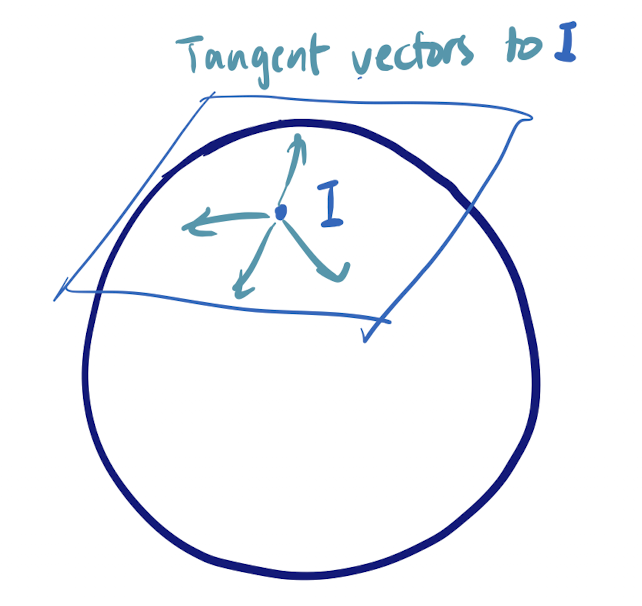
\includegraphics[width=5cm]{Lecture Files and Images/lec32-tangentvector.png}
\end{center}

There are three approaches to rigorously defining tangent vectors. \begin{enumerate}
    \item  The approach taken so far is that a tangent vector will be given by a matrix $A \in \text{Mat}_{n \by n}(\RR)$ such that the corresponding one-parameter group $e^{tA} \in G$ for all $t \in \RR$.\footnote{Every matrix $A$ will define some path in $GL_n;$ if the entire path lives in $G,$ then we can think of $A$ as a tangent vector.}
    \item The second approach is more general, and builds on the idea that a one-parameter group is the trajectory of a particle moving in $G$ in a specific way defined by $\varphi.$ Instead of taking a path that happens to be a homomorphism, take any differentiable path\footnote{Any matrix-valued function} from some interval $f: (-\varepsilon, \varepsilon) \rto GL_n(\RR)$ such that $f(0) = I$ and $f(t) \in (G)$ for all $t.$ Then a tangent vector is simply the velocity at time $t = 0$, $f'(0) \in \text{Mat}_{n \by n}(\RR).$\footnote{The idea is that all the paths through the identity will give velocity vectors (with lots of redundancy), which we will consider as tangent vectors.}
\end{enumerate}

It is not obvious, but it turns out that the first definition is equivalent to the second definition, giving the same subsets of matrices $A$ as tangent vectors. For the first definition, the advantage is that each tangent vector corresponds to only one path through the identity, so there is a bijection. The second approach gives lots of paths through the identity that have a given velocity vector, but it turns out that it is easier to use it to show that the set of tangent vectors actually forms a vector space, called the tangent space.\footnote{There is actually more structure on it, which we will talk about on Friday.}

\begin{enumerate} %START NUMBWRING AT 3
\setcounter{enumi}{2}
    \item Suppose $G$ is defined by polynomial constraints on the matrix entries.\footnote{This approach is not necessary for this class, but it is fun, so we will do it.} For example, the constraints could be that it is upper triangular; then $a_{ij} = 0$ for all $i > j$ is a bunch of polynomial conditions on the matrix entries. Orthogonality can also be phrased as a polynomial condition.
    
    Then, when working with polynomials, the derivative can be mimicked without actually needing to know analysis. We work with an object $\RR[\varepsilon] \coloneqq \RR + \RR \varepsilon$ where $\varepsilon^2 = 0.$\footnote{Here $\varepsilon$ is not some number in $\RR,$ so it is not actually true that $\varepsilon$ must be 0; it is simply a formal construct where we impose the condition that $\varepsilon^2 = 0.$ It is similar to the definition of $i = \sqrt{-1}$; there is no such real number, so we simply define some number satisfying this property. In the same way, we simply define $\RR[\varepsilon]$ to be $\RR + \RR \varepsilon$ for some object $\varepsilon$ satisfying $\varepsilon^2 = 0.$} 
    
    This allows us to define a derivative without actually taking any limits. For example, for $f(x)  = x^2 + 2x,$ evaluating $f$ on $x + \varepsilon \in R[\varepsilon]$ will give
    \begin{align*}
           f(x + \varepsilon) &= (x + \varepsilon)^2 + 2(x + \varepsilon) \\
           &= x^2 + 2x\varepsilon + \varepsilon^2 + 2x + 2\varepsilon\\
           &= x^2 + 2x\varepsilon + 2x + 2\varepsilon\\
           &= (x^2 + 2x) + (2x + 2)\varepsilon.
    \end{align*}
    So with this funky multiplication, any terms of order more than two in $\varepsilon$ disappear, and we get $\frac{f(x + \varepsilon) - f(x)}{\varepsilon} = f'(x),$ even though we haven't actually defined the derivative from an analysis perspective. 
\end{enumerate}

The upshot is that to find $A \in \text{Mat}_{n \by n}(\RR)$, we simply look at $A$ with the property that $I_n + \varepsilon A$, the identity matrix perturbed by $A$, satisfies the same system of equations defining $G$, but in the sense of the funky multiplication of $\RR[\varepsilon]$, where $\varepsilon^2 = 0.$ We'll explain this more on Friday.

\newpage

\lhead{Lecture 33: Lie Groups}
%MIT OpenCourseWare: https://ocw.mit.edu
%RES.18-011 Algebra I Student Notes, Fall 2021
%License: Creative Commons BY-NC-SA 
%For information about citing these materials or our Terms of Use, visit: https://ocw.mit.edu/terms.

\section{Lie Groups}

\subsection{Review}
Last time, we discussed one-parameter groups $G \leq GL_n(\RR).$ We started thinking about tangent vectors to the group, based at some identity.

\begin{definition}
The collection of all tangent vectors at $I \subset G$, called the \textbf{tangent space}, can be characterized in multiple ways. We call this $\lie(G),$ pronounced "lee." 
\end{definition}

\begin{center}
    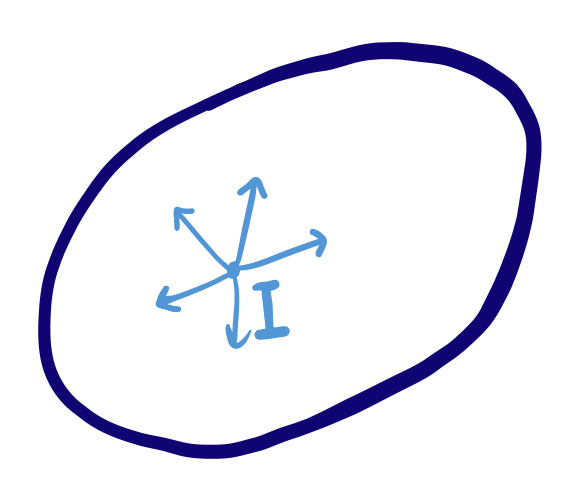
\includegraphics[width=6cm]{Lecture Files and Images/lec33-1.png}
\end{center}

\begin{enumerate}
    \item The first definition is the most familiar one. The tangent vectors are the matrices such that the associated one-parameter subgroup lies in $G$. We found that there is a bijection between matrices and one-parameter groups lying in $G.$ \[\lie(G) = \{A \in \matnn(\RR) : e^{tA} \in G, t \in \RR\}\]
    \item More generally, we consider any path inside the group through the identity, not just a one-parameter group, and take $A$, the velocity at the identity, to be a tangent vector.\footnote{For definition 1, we know all the 1-parameter subgroups, but for definition 2, there are lots of other possible paths. So for definition 1, there is a bijection between the matrices $A$ and the one-parameter groups, while for definition 2, there are lots of different paths with the same tangent vector as the velocity. Definition 2 does not use the fact that $G$ is a group.}
    

    \[\lie(G) = \{A \in \matnn(\RR): \exists f:(-\varepsilon, \varepsilon) \rto G, f(0) = I, f'(0) = A\}\]
    \begin{center}
        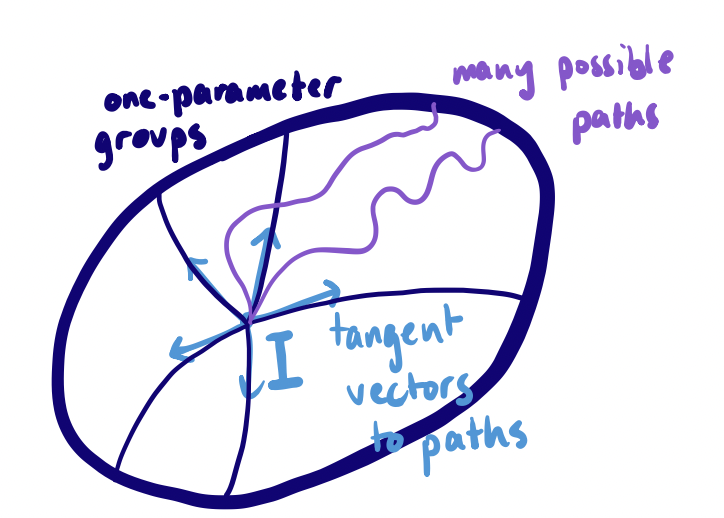
\includegraphics[width=7cm]{Lecture Files and Images/lec33-2.png}
    \end{center}
    \item The third approach is slightly stranger. It is less general, and requires $G$ to be defined by polynomial constraints.\footnote{For example, setting the determinant to be 1 is some complicated polynomial constraint.} In this case, we take this strange construction \[\RR[\varepsilon] = \RR \oplus \RR \varepsilon = \{a + b \varepsilon: a, b \in \RR\},\] where we define the multiplication to be such that \[\varepsilon^2 = 0.\footnote{This is similar to how we could define the complex numbers, where we set $i^2 = -1.$}\] If $f$ is a polynomial, then we can set, formally, the derivative to be \[f'(x) = f(x + \varepsilon) - f(x).\] This is a way of thinking about the derivative without limits, for polnyomials. Then, we take \[\lie(G) = \{A \in \matnn : I + \varepsilon A \text{ satisfies the polynomial constraints defining } G\}.\]
\end{enumerate}

\subsection{Lie Groups}
These definitions are quite abstract, so let's see them in action for $O_n.$ 
\begin{example}
Let $G = O_n,$ the set of matrices such that $A^TA = I.$
\end{example}
\begin{enumerate}
    \item The Lie group, as we have seen in the previous lecture, is \[\lie(O_n) = \{A: A^T = -A\}.\] These are the \textbf{skew-symmetric} matrices.
    \item Consider a path passing through the identity at zero: \[f: (-\varepsilon, \varepsilon) \rto O_n\] such that $f(0) = I.$ By the definition of an orthogonal matrix, \[f(t)^T\cdot f(t) = I.\] Taking the derivative, \[f'(t)^T \cdot f(t) = f(t)^T \cdot f'(t) = 0,\] and taking $t = 0$ gives $A^TI + IA = 0,$ and thus \[A^T = -A.\] So the same condition holds.
    \item The condition that $A^TA = I$ is a set of complicated polynomial conditions. From definition 3), the Lie group consists of matrices $A$ such that \[(I + \varepsilon A)^T(I + \varepsilon A) = I,\] using the rule that $\varepsilon^2 = 0.$ Multiplying this out, \[I + \varepsilon A^T + \varepsilon A + \varepsilon^2 A^TA,\] and taking $\varepsilon^2 = 0,$ \[I + \varepsilon A^T + \varepsilon A = I,\] which implies that \[A^T = -A\] after dividing both sides by $\varepsilon.$
\end{enumerate}

All three definitions lead to the same Lie group, despite being very different. The third definition is useful because it makes sense even without working over the real numbers, and works for any group defined by polynomial constraints!\footnote{The intuition for this third definition is that it is essentially using the Taylor expansion of the path through the identity, and ignoring third order and higher terms.} For example, the Lie group can be defined for orthogonal matrices over finite fields.

Here are some non-obvious facts about these characterizations of the tangent space at the identity. 
\begin{proposition}
For $\lie(G):$
\begin{itemize}
    \item All three definitions are actually equivalent.
    \item For a group $G,$ $\lie(G)$ is actually a vector \emph{subspace} of $\text{Mat}_{n \by n}(\RR).$
\end{itemize}
\end{proposition}

It is surprising that $\lie(G)$ is a vector space, since the matrix exponential does not generally behave well with respect to addition if $A$ and $B$ do not commute.\footnote{Using the first definition, it is not clear that $e^{tA} + e^{tB}$ can be written as $e^{tC}$.}


\subsection{Manifolds}
In order to understand Lie groups, we have to think about the notion of a \emph{manifold.} For this section, the discussion will be less rigorous and precise, and it is okay not to understand all the definitions; we are just providing the flavor of concepts that will show up in later classes.
\begin{definition}
For $M$ a subset of $\RR^n,$ $M$ is a \textbf{(differentiable) manifold of dimension $d$} if for each $x \in M,$ there exists an open set containing $x$ $V \subseteq M$, an open ball $U \subset \RR^d$\footnote{An open ball is a subset of $\RR^d$ of the form $U = \{x : |x| < \delta\}$ for some $\delta.$}, and a continuous (differentiable) bijection $f: U \rto V.$

\begin{center}
    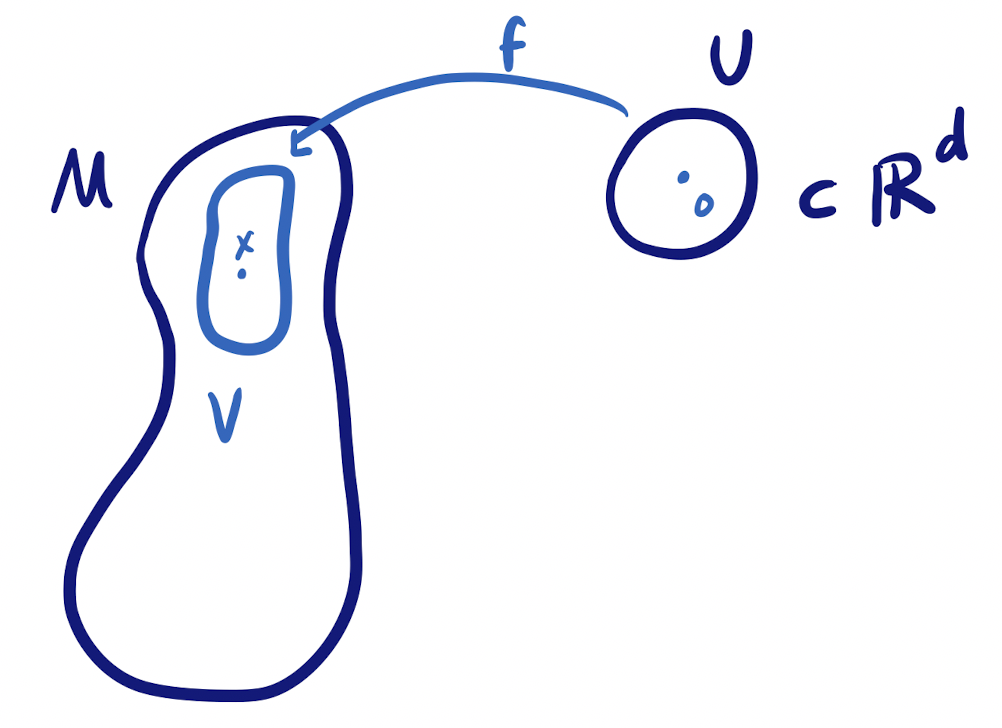
\includegraphics[width=8cm]{Lecture Files and Images/lec33-manifold.png}
\end{center}

\end{definition}



Globally, a $d$-dimensional does not look like $\RR^d,$ but locally, it does. The circle is an example of a 1-dimensional manifold; at each point on the circle, there is really only one direction to move in.


\begin{example}[Circle]

Consider some interval on the real line. Then, it is possible to write down some function bijectively mapping that interval to some other interval on the circle. This can happen around any point on the circle, so it is a manifold.

\begin{center}
    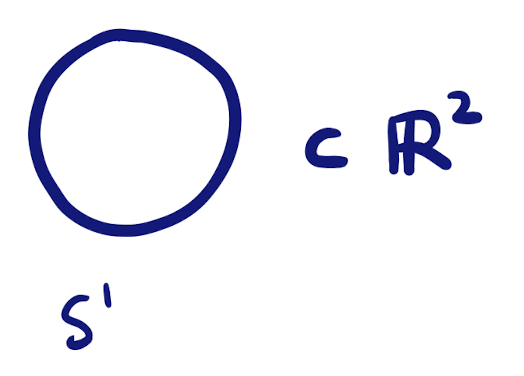
\includegraphics[width=6cm]{Lecture Files and Images/lec33-circol.png}
\end{center}
\end{example}

Loosely, for definition 2, we have tangent vectors at $0$ in $U \subset \RR^d$ corresponding to tangent vectors at $x$ in $M,$ which in a way brings the vector space structure from $\RR^d$ to $M.$ 

A non-example would be the union of the $x$-axis and the $y$-axis, since at the origin, there is an intersection that does not look like an interval. There are two directions to move in, instead of one direction. 

\begin{center}
    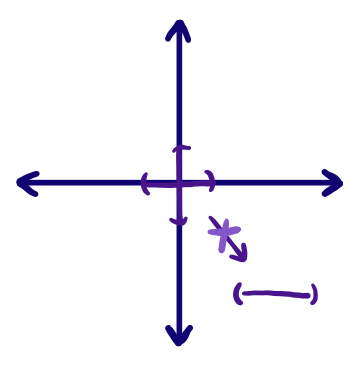
\includegraphics[width=6cm]{Lecture Files and Images/lec33-3.png}
\end{center}


All our examples of $G \leq GL_n(\RR)$ are manifolds, not just groups. This requires some argument, but it is true. 

\subsection{Lie Bracket}

For every group $G,$ there is a corresponding vector space structure $\lie(G) \subset \matnn(\RR) = \lie(GL_n(\RR)).$ In fact, $\lie(G)$ carries some extra structure. The multiplication structure $A, B \rightsquigarrow AB \in \matnn(R)$ does \emph{not} preserve $\lie(G)$; if $A, B \in \lie(G),$ it does \emph{not} mean that $AB \in \lie(G).$ For example, $\lie(O_n) = \{A: A^T = -A\},$ so for $A, B \in \lie(G),$ $(AB)^T = B^TA^T = BA,$ which is not usually equal to $-AB.$ However, a very similar structure \emph{does} preserve the Lie group.

\begin{definition}[Lie Bracket]
Let the Lie bracket of $A, B \in \matnn(R)$ be \[[A, B] \coloneqq AB - BA \in \matnn(R).\]
\end{definition}

% The Lie bracket %idk say something about it

\begin{theorem}
For any $G \leq GL_n,$ the Lie group $G \subseteq \matnn(R)$ is preserved by the Lie bracket:
\[
A, B \in \lie(G) \rightarrow [A, B] \in \lie(G) %probably edit this one lol ?? what does this mean
\]
\end{theorem}

The Lie group is not just a vector space --- it is actually a vector space with some weirdo multiplication on it!

The Lie bracket can be seen in action for some of the Lie groups we have seen already.
\begin{example}
For $G = O_n,$ $\lie(O_n) = \{A: A^T = -A\}.$ Then for $A, B \in \lie(O_n),$ $[A, B] = AB - BA,$ and
\[
[A, B]^T = B^TA^T -A^TB^T = BA -AB = -[A, B].
\]
So $[A, B] \in \lie(O_n).$
\end{example}
\begin{example}
For $SL_n(\RR),$ $\lie(SL_n(\R)) = \{A: \text{trace}(A) = 0\}.$ For matrices $A, B,$ $\text{trace}(AB) = \text{trace}(BA),$ and so $\text{trace}([A, B]) = 0.$ %whats WRONGGGG
\end{example}

The commutator in the group corresponds to the Lie bracket. %what does this mean
\begin{proof}
For $A, B \in \lie(G),$ then consider $e^{tA} \in G$ and $e^{sB} \in G.$ Then we know that 
\[
e^{tA} e^{sB} e^{-tA}e^{-sB} \in G,
\]
and Taylor expanding gives
\[
(I + tA + \cdots)(I + sB + \cdots)(I -tA + \cdots)(I - sB + \cdots) \in G,
\]
which, to the first order, gives 
\[
I + st[A, B] + \cdots \in G.
\]

Then, taking the derivative at $0$ gives 
\[
[A, B] \in \lie(G).
\]%WHO is at 0?? LOL s or t???
\end{proof}

The Lie bracket comes from the fact that the group is closed under multiplication and taking the derivative at 0 for that. As a corollary, if $G$ is abelian\footnote{For example, diagonal matrices}, then the Lie bracket is identically 0 on all of $G.$ In some way, for an arbitrary group $G,$ the Lie bracket "measures" the failure of the group to be abelian. 

We started out with groups that we cared about (matrix groups), looked at the set of tangent vectors, which is the same as the set of one-parameter groups, and looked at the vector space structure which also has a funky Lie bracket, and now we will look at properties of this bracket.

Here are some nice properties of the Lie bracket.
\begin{itemize}
    \item \textbf{Antisymmetry.} $[A, B] = -[B, A]$
    \item \textbf{The Jacobi identity.} We have $[[A, B], C] + [[B, C], A] + [[C, A], B] = 0.$ It is true simply when expanding. This also comes from a property of the group; we won't do it but you can get it by staring at a more complicated version of how we derived the Lie bracket. %explain this better
\end{itemize}

\begin{definition}
A \textbf{Lie algebra} (over $\RR$) is a vector space $V$ with a Lie bracket $[\cdot, \cdot]: V \by V \rto V$ satisfying $[A, B] = -[B, A]$ and the Jacobi identity.
\end{definition}

On the homework, we see that $\RR^2$ with the cross product is a Lie algebra, and it is $\lie(SO_3) = \lie(SU_2).$

If $G$ is a group that is also a manifold, it is called a Lie group, and if $G$ is a Lie group, it can be replaced with $\lie(G)$, a Lie algebra, which is simply a vector space with a weird multiplication on it, which is a lot easier to study. However, the Lie algebra carries a \emph{lot} of information about $G.$ 

\begin{theorem}
Given a Lie algebra (finite dimensional over $\RR$) $V$, there exists a \emph{unique} Lie group $G$ such that $\lie(G) = V.$
\end{theorem}

Lie theory ends up being a very powerful tool in the study of understanding groups.

% Lie groups are symmetries of physical objects no more geometry or group theory. this is step 0 in a whole program of how to ubderstand groups. ok we are done for today.
\newpage

\lhead{Lecture 34: Simple Linear Groups}
%MIT OpenCourseWare: https://ocw.mit.edu
%RES.18-011 Algebra I Student Notes, Fall 2021
%License: Creative Commons BY-NC-SA 
%For information about citing these materials or our Terms of Use, visit: https://ocw.mit.edu/terms.

\section{Simple Linear Groups}

\subsection{Review}

Last time, we took a group $G \leq GL_n(\mathbb{R})$ and looked at $\operatorname{Lie}(G)$, the vector space of tangent vectors at the identity. We had lots of different definitions, but the most familiar way is to think of $\operatorname{Lie}(G)$ as all the matrices that provide one-parameter groups inside of $G.$ The key point was that not only is $\operatorname{Lie}(G)$ a vector space, but it also has some extra structure: the Lie bracket $[A, B] = AB - BA$, which is a skew-symmetric multiplication on the vector space. This is a new operation, but it also arises naturally from considering multiplication on $G$, and sort of taking its derivative. The Lie bracket measures the failure of $G$ to be commutative.

We don't actually need $G$ to be a subgroup of $GL_n(\mathbb{R})$ in order to do this. For any group with a manifold structure, called a \textbf{Lie group}, we can look at the tangent vectors through the identity, and we get a vector space which also has a bracket multiplication, which is its \textbf{Lie algebra} $\operatorname{Lie}(G)$. 

\begin{question}
    Can you recover the group from its Lie algebra?
\end{question}

\begin{ans}
    In general, the answer is no. For example, $SU_2$ and $SO_3$ have the same Lie algebra. But it turns out that if two groups have the same Lie algebra, they're related to each other -- here $SU_2$ and $SO_3$ differ by a ``finite amount'' (we have a two-to-one surjection $SU_2 \to SO_3$), and you can show something similar is true in general. In fact, if you require the group to be simply connected, then there is a unique group with a given Lie algebra. You can then use this to study all the groups with a given Lie algebra. 
\end{ans}

This ends up being a powerful tool because now in order to understand a group with a manifold structure, we can instead try to understand its Lie algebra, which is an easier problem; and then figure out how to go backwards. 

\subsection{Simple Linear Groups}

Recall that a group is \textbf{simple} if its only normal subgroups are the trivial group and the whole group. You can think of simple groups as building blocks for more complicated groups -- if you have a group that isn't simple, then you can understand it by understanding the normal subgroup and its quotient group. But if you have a simple group, you can't break it down further. 

\begin{qq}
Which $G \leq GL_n(\mathbb{R})$ are simple?
\end{qq}

We'll look at two groups: $SU_2$ and $SL_2$. 

\subsection{The Special Unitary Group}

First we'll look at whether $SU_2$ is simple. The answer is no -- the center of a group (the set of elements which commute with everything) is always a normal subgroup. But the center of $SU_2$ is $\pm I$, which is nontrivial. 

But it turns out that's essentially the only thing that can happen: 

\begin{theorem}\label{su2normal}
    If $N \trianglelefteq SU_2$, then $N$ must be $\{I\}$, $SU_2$, or $\{\pm I\}$.
\end{theorem}

So then in order to produce a simple group, we can quotient out by this center:

\begin{corollary}\label{so3simple}
    The quotient $SU_2/\{\pm I\}$ is simple. 
\end{corollary}

This quotient is actually $SO_3$: we have a surjective homomorphism $SU_2 \to SO_3$ (from the conjugation action on the equator), and the kernel is exactly $\{\pm I\}$. So in particular, $SO_3$ is simple. 

\begin{proof}[Proof of Corollary \ref{so3simple}]
    This follows from the Correspondence Principle: we have a surjection $\varphi : SU_2 \to SO_3$. So for any normal subgroup $N \trianglelefteq SO_3$, its pre-image is a subgroup of $SU_2$, which is also normal and contains the kernel $\{\pm I\}$. But any normal subgroup of $SU_2$ containing the kernel is equal to either the kernel or the whole group, which means the initial normal subgroup in $SO_3$ is either the identity or the entire group (by taking the image under $\varphi$). 
\end{proof}

\begin{proof}[Proof of Theorem \ref{su2normal}]
    We can use the geometric intuition of what $SU_2$ looks like. It's a $3$-sphere in $4$-dimensional space, and its conjugacy classes are exactly the latitudes -- the $2$-spheres we get from taking horizontal slices. 

    Suppose we have $N \trianglelefteq SU_2$, and some element $Q \in N$ which is not $\pm I$. We'd like to show that $N$ must then be the entire group. 
    
    % \begin{center}
    %     \begin{asy}
    %         unitsize(2.5cm);
    %         draw(circle((0, 0), 1));
    %         real latc(real a, real b) {
    %             return sqrt((1 - a^2)*(a^2 - b^2)/a^2);
    %         }
    %         path latitude(real a, real b) {
    %             return ellipse((0, latc(a, b)), a, b);
    %         }
    %         draw(latitude(1, 0.2), dotted);
    %         real aq = 0.8;
    %         real bq = aq/5;
    %         path latq = latitude(aq, bq);
    %         draw(latq, heavycyan+dotted);
    %         pair Q = intersectionpoints(latq, (0.5, 2)--(0.5, -2))[1];
    %         dot("$Q$", Q, dir(270));
    %         pair I = dir(90);
    %         dot("$I$", I, dir(90));
    %     \end{asy}
    % \end{center}
    
    \begin{center}
        \begin{asy}
            unitsize(2.5cm);
            draw(circle((0, 0), 1));
            real latc(real a, real b) {
                return sqrt((1 - a^2)*(a^2 - b^2)/a^2);
            }
            path lat2(real a, real b) {
                return shift((0, latc(a, b)))*scale(a, b)*arc((0, 0), 1, 0, 180);
            }
            path lat1(real a, real b) {
                return shift((0, latc(a, b)))*scale(a, b)*arc((0, 0), 1, 180, 360);
            }
            draw(lat1(1, 0.2), gray);
            draw(lat2(1, 0.2), gray+dashed);
            real aq = 0.8;
            real bq = aq/5;
            draw(lat1(aq, bq), heavycyan);
            draw(lat2(aq, bq), heavycyan+dashed);
            pair Q = intersectionpoint(lat1(aq, bq), (0.5, 2)--(0.5, -2));
            dot("$Q$", Q, dir(270));
            pair I = dir(90);
            dot("$I$", I, dir(90));
        \end{asy}
    \end{center}
    
    Since $N$ is normal, everything conjugate to $Q$ must also be in $N$. If $\trace(Q) = 2c$, then $\operatorname{Lat}_c$ is the conjugacy class of $Q$, so this entire latitude must be inside $N$. (This latitude is a $2$-sphere of positive radius, since $Q$ is not $\pm I$.) 

    Now we can take this $2$-sphere, and translate it to pass through the identity: consider $Q^{-1}\operatorname{Lat}_c$, which is a $2$-sphere (of positive radius) passing through the north pole $I$. This must also be contained inside $N$ (since $Q$ and $\operatorname{Lat}_c$ are both contained inside $N$). 
    
    % \begin{center}
    %     \begin{asy}
    %         unitsize(2.5cm);
    %         draw(circle((0, 0), 1));
    %         real latc(real a, real b) {
    %             return sqrt((1 - a^2)*(a^2 - b^2)/a^2);
    %         }
    %         path latitude(real a, real b) {
    %             return ellipse((0, latc(a, b)), a, b);
    %         }
    %         draw(latitude(1, 0.2), dotted);
    %         real aq = 0.8;
    %         real bq = aq/5;
    %         path latq = latitude(aq, bq);
    %         draw(latq, heavycyan+dotted);
    %         pair Q = intersectionpoints(latq, (0.5, 2)--(0.5, -2))[1];
    %         dot("$Q$", Q, dir(270));
    %         pair I = dir(90);
    %         dot("$I$", I, dir(90));
    %         real qheight = latc(aq, bq);
    %         real theta = aCos(qheight);
    %         path translatq = rotate(-theta)*latq;
    %         draw(translatq, heavyred+dotted);
    %     \end{asy}
    % \end{center}
    
    \begin{center}
        \begin{asy}
            unitsize(2.5cm);
            draw(circle((0, 0), 1));
            real latc(real a, real b) {
                return sqrt((1 - a^2)*(a^2 - b^2)/a^2);
            }
            path lat2(real a, real b) {
                return shift((0, latc(a, b)))*scale(a, b)*arc((0, 0), 1, 0, 180);
            }
            path lat1(real a, real b) {
                return shift((0, latc(a, b)))*scale(a, b)*arc((0, 0), 1, 180, 360);
            }
            draw(lat1(1, 0.2), gray);
            draw(lat2(1, 0.2), gray+dashed);
            real aq = 0.8;
            real bq = aq/5;
            draw(lat1(aq, bq), heavycyan);
            draw(lat2(aq, bq), heavycyan+dashed);
            pair Q = intersectionpoint(lat1(aq, bq), (0.5, 2)--(0.5, -2));
            dot("$Q$", Q, dir(270));
            pair I = dir(90);
            dot("$I$", I, dir(90));
            real qheight = latc(aq, bq);
            real theta = aCos(qheight);
            draw(rotate(-theta)*lat1(aq, bq), heavyred);
            draw(rotate(-theta)*lat2(aq, bq), heavyred+dashed);
        \end{asy}
    \end{center}

    Now start at $I$, and take a nontrivial path inside this two-sphere. Write this path as $f(t)$ for $0 \leq t \leq \varepsilon$, where we have $f(t) \in Q^{-1}\operatorname{Lat}_c$ for all $t$, and $f(0) = I$, while $f(t) \neq I$ for $t > 0$. 
    
    \begin{center}
        \begin{asy}
            unitsize(2.5cm);
            draw(circle((0, 0), 1));
            real latc(real a, real b) {
                return sqrt((1 - a^2)*(a^2 - b^2)/a^2);
            }
            path lat2(real a, real b) {
                return shift((0, latc(a, b)))*scale(a, b)*arc((0, 0), 1, 0, 180);
            }
            path lat1(real a, real b) {
                return shift((0, latc(a, b)))*scale(a, b)*arc((0, 0), 1, 180, 360);
            }
            draw(lat1(1, 0.2), gray);
            draw(lat2(1, 0.2), gray+dashed);
            real aq = 0.8;
            real bq = aq/5;
            draw(lat1(aq, bq), heavycyan);
            draw(lat2(aq, bq), heavycyan+dashed);
            pair Q = intersectionpoint(lat1(aq, bq), (0.5, 2)--(0.5, -2));
            dot("$Q$", Q, dir(270));
            pair I = dir(90);
            dot("$I$", I, dir(90));
            real qheight = latc(aq, bq);
            real theta = aCos(qheight);
            draw(rotate(-theta)*lat1(aq, bq), heavyred);
            draw(rotate(-theta)*lat2(aq, bq), heavyred+dashed);
            path f = rotate(-theta)*shift((0, qheight))*scale(aq, bq)*arc((0, 0), 1, 180, 240);
            draw(f, deepred+linewidth(2));
        \end{asy}
    \end{center}
    
    Then $f(t)$ is contained in $Q^{-1}\operatorname{Lat}_c$, and therefore inside $N$. And the north pole is the only point in the sphere with trace $2$, so $\trace(f(t)) < 2$ for all $t > 0$. This means there exists some $\delta > 0$ such that for all $2 - \delta < c < 2$, there exists $t$ such that $\trace(f(t)) = c$. 

    But once we find that $N$ contains one point on a given latitude, then $N$ must contain \emph{every} point on that latitude (because $N$ is normal, so it must contain the entire conjugacy class of that point). So this means for every $c$ such that $2 - \delta < c < 2$, the latitude $\operatorname{Lat}_{c/2}$ is contained inside $N$. 
    
    \begin{center}
        \begin{asy}
            unitsize(2.5cm);
            draw(circle((0, 0), 1));
            real latc(real a, real b) {
                return sqrt((1 - a^2)*(a^2 - b^2)/a^2);
            }
            path lat2(real a, real b) {
                return shift((0, latc(a, b)))*scale(a, b)*arc((0, 0), 1, 0, 180);
            }
            path lat1(real a, real b) {
                return shift((0, latc(a, b)))*scale(a, b)*arc((0, 0), 1, 180, 360);
            }
            draw(lat1(1, 0.2), gray);
            draw(lat2(1, 0.2), gray+dashed);
            real aq = 0.8;
            real bq = aq/5;
            draw(lat1(aq, bq), heavycyan);
            draw(lat2(aq, bq), heavycyan+dashed);
            pair Q = intersectionpoint(lat1(aq, bq), (0.5, 2)--(0.5, -2));
            dot("$Q$", Q, dir(270));
            pair I = dir(90);
            dot("$I$", I, dir(90));
            real qheight = latc(aq, bq);
            real theta = aCos(qheight);
            draw(rotate(-theta)*lat1(aq, bq), heavyred);
            draw(rotate(-theta)*lat2(aq, bq), heavyred+dashed);
            path f = rotate(-theta)*shift((0, qheight))*scale(aq, bq)*arc((0, 0), 1, 180, 240);
            draw(f, deepred+linewidth(2));
            draw(lat1(0.2, 0.04), heavycyan);
            draw(lat2(0.2, 0.04), heavycyan+dashed);
            draw(lat1(0.4, 0.08), heavycyan);
            draw(lat2(0.4, 0.08), heavycyan+dashed);
            draw(lat1(0.6, 0.12), heavycyan);
            draw(lat2(0.6, 0.12), heavycyan+dashed);
        \end{asy}
    \end{center}

    This means we have an entire neighborhood of the identity that's contained inside $N$ -- any point $A \in SU_2$ with $\trace(A) > 2 - \delta$ is contained inside $N$. 
    
    Now we're almost done: we want to show that once we have a neighborhood of the identity, we have all points. To do this, we can look at the longitudes: pick some $v$ on the equator, and look at $\operatorname{Long}_v \leq SU_2$. Every point on the three-sphere is in some longitude, so it suffices to show that every longitude is contained in $N$. 
    
    \begin{center}
        \begin{asy}
            unitsize(2.5cm);
            draw(circle((0, 0), 1));
            real latc(real a, real b) {
                return sqrt((1 - a^2)*(a^2 - b^2)/a^2);
            }
            path lat2(real a, real b) {
                return shift((0, latc(a, b)))*scale(a, b)*arc((0, 0), 1, 0, 180);
            }
            path lat1(real a, real b) {
                return shift((0, latc(a, b)))*scale(a, b)*arc((0, 0), 1, 180, 360);
            }
            draw(lat1(1, 0.2), gray);
            draw(lat2(1, 0.2), gray+dashed);
            real aq = 0.8;
            real bq = aq/5;
            //draw(lat1(aq, bq), heavycyan);
            //draw(lat2(aq, bq), heavycyan+dashed);
            pair Q = intersectionpoint(lat1(aq, bq), (0.5, 2)--(0.5, -2));
            //dot("$Q$", Q, dir(270));
            pair I = dir(90);
            dot("$I$", I, dir(90));
            real qheight = latc(aq, bq);
            real theta = aCos(qheight);
            //draw(rotate(-theta)*lat1(aq, bq), heavyred);
            //draw(rotate(-theta)*lat2(aq, bq), heavyred+dashed);
            path f = rotate(-theta)*shift((0, qheight))*scale(aq, bq)*arc((0, 0), 1, 180, 240);
            //draw(f, heavyred+linewidth(1.7));
            draw(lat1(0.2, 0.04), heavycyan);
            draw(lat2(0.2, 0.04), heavycyan+dashed);
            draw(lat1(0.4, 0.08), heavycyan);
            draw(lat2(0.4, 0.08), heavycyan+dashed);
            draw(lat1(0.6, 0.12), heavycyan);
            draw(lat2(0.6, 0.12), heavycyan+dashed);
            real vr = 0.4;
            draw(rotate(90)*lat1(1, 0.4), deepgreen+dashed);
            draw(rotate(90)*lat2(1, 0.4), deepgreen);
        \end{asy}
    \end{center}
    
    But this longitude is the circle \[\{\cos \theta I + \sin \theta v \mid 0 \leq \theta < 2\pi\}.\] And we know that if $\theta$ is small enough, then the point $\rho_\theta$ corresponding to $\theta$ is in $N$ (meaning there exists $\varepsilon$ such that $\rho_\theta \in N$ for all $|\theta| < \varepsilon$). 
    \begin{center}
        \begin{asy}
            import geometry;
            unitsize(2.5cm);
            draw(circle((0, 0), 1));
            dot("$I$", dir(90), dir(90));
            dot("$\rho_\theta$", dir(50), dir(50));
            draw(dir(90)--(0, 0)--dir(50));
            markangle("$\theta$", radius = -8, dir(90), (0, 0), dir(50));
            draw(arc((0, 0), 1, 70, 110), heavycyan+linewidth(1.7));
            draw(0.95*dir(70)--1.05*dir(70), heavycyan+linewidth(1.7));
            draw(0.95*dir(110)--1.05*dir(110), heavycyan+linewidth(1.7));
        \end{asy}
    \end{center}

    Now we can take $\rho_\theta$ for small $\theta$, and multiply it by itself repeatedly to cover the entire circle: for any $\varphi \in [0, 2\pi)$, there is some $M$ such that $\left|\frac{\varphi}{M}\right| < \varepsilon$. Then $\rho_{\phi/M}$ is in $N$, which means $\rho_\varphi = (\rho_{\varphi/M})^M$ is in $N$ as well. 
    
    So now every longitude is in $N$, and since every point is in a longitude, this means all of $SU_2$ is in $N$. 
\end{proof}

\begin{note}
This is a really hands-on argument; we used the fact that we have both a geometric and group-theoretic understanding of what $SU_2$ is. 
\end{note}

\subsection{The Special Linear Group}

Now we'll look at $SL_2(\mathbb{C})$ -- the group of $2 \times 2$ matrices with determinant $1$. 

Again, $\pm I$ is the center of $SL_2(\mathbb{C})$, so the most we could ask for is that if we quotient out by this normal subgroup, we get a simple group. It turns out that this is the case, and it actually works for \emph{any} field $F$, not just the complex numbers:

\begin{theorem} \label{sl2simple}
    For any field $F$ with $|F| \geq 4$, the quotient $SL_2(F)/\{\pm I\}$ is simple. 
\end{theorem}

This quotient is sometimes called $PSL_2(F)$. 

We're no longer in a geometric setting ($F$ can be a finite field), so the proof won't be geometric like the previous one; instead, we'll get our hands on generators and relations. 

\begin{note}
The theorem is false over $\mathbb{F}_2$ and $\mathbb{F}_3$. This is similar to how when we looked at the alternating groups, we saw that $A_n$ is simple for all $n \geq 5$, but $A_4$ and $A_3$ are not simple. In both cases, we have a family of groups where the first couple may be counterexamples, but eventually they all become simple.
\end{note}

\begin{proof}[Proof of Theorem \ref{sl2simple}]
    We'll prove this in the case where $|F| > 5$ (there's only two remaining cases, which can be checked by hand). It suffices to prove that if we have a normal subgroup $N \trianglelefteq SL_2(F)$, then $N$ is either $\{I\}$, $\{\pm I\}$, or $SL_2(F)$ -- then this implies the quotient is simple by the same argument as before, using the Correspondence Principle. 

    We'll begin with a few lemmas about the field:
    
    \begin{lemma}
        Given $a \in F$, the equation $x^2 = a$ has at most $2$ solutions. 
    \end{lemma}
    
    This seems obvious, but it's possible to have more solutions in $\mathbb{Z}/n\mathbb{Z}$ if $n$ is not prime. So it matters that $F$ is a field. 
    
    \begin{proof}
        If we have two solutions $x$ and $y$, then $x^2 = y^2$, so \[(x + y)(x - y) = 0.\] But because $F$ is a field, if two elements multiply to $0$, then one of them is $0$. So either $x = y$ or $x = -y$; this means if there's one solution, then there's at most one other solution. 
    \end{proof}

    \begin{lemma}
        If $|F| > 5$, then there exists some $r \in F$ such that $r^2$ is not $0$, $1$, or $-1$. 
    \end{lemma}

    \begin{proof}
        There's at most one square root of $0$, two square roots of $1$, and two square roots of $-1$. So there are at most five bad elements; and as long as there are more than $5$ elements in the field, we can find some good element (whose square isn't $0$ or $\pm 1$).
    \end{proof}

    Now we'll prove the main theorem. Fix an element $r$ with $r^2 \not\in\{0, 1, -1\}$. Assume that we have a normal subgroup $N \trianglelefteq SL_2(F)$ containing some element other than $\pm I$; then we'll show that $N$ is the entire group. 
    
    \begin{claim}
        We can find some $B \in N$ with distinct eigenvalues. 
    \end{claim}

    \begin{proof}
        Pick some $A \in N$, with $A \neq \pm I$. Then $A$ is not a scalar matrix, so there is some vector $v_1 \in F^2$ which is not an eigenvector of $A$. Then take $v_2 = Av_1$. Since $v_1$ is not an eigenvector, $v_1$ and $v_2$ are linearly independent, so $\{v_1, v_2\}$ is a basis for $F^2$. 
    
        Now define $P \in GL_2(F)$ with the property that $Pv_1 = rv_1$ and $Pv_2 = r^{-1}v_2$. Then $P$ is diagonal in the basis $\{v_1, v_2\}$, and its eigenvalues are $r$ and $r^{-1}$. So the determinant of $P$ is $1$, which means $P \in SL_2(F)$. 
    
        We don't know whether $P$ is in $N$. But we can define $B = APA^{-1}P^{-1}$. We claim that $B$ is inside $N$ -- we know $A$ is in $N$. Meanwhile, $PA^{-1}P^{-1}$ is the conjugate of an element of $N$, so it must also be in $N$ (since $N$ is normal). Since $N$ is a subgroup, their product must be in $N$ as well. 
    
        But we have \[Bv_2 = APA^{-1}P^{-1}v_2 = APA^{-1}rv_2 = APrv_1 = Ar^2v_1 = r^2v_2.\] So $r^2$ is an eigenvalue of $B$, and $r^{-2}$ is the other eigenvalue (because $\det B = 1$). By our choice of $r$, we have $r^2 \neq r^{-2}$, since $r^2 \neq \pm 1$. So this concludes the first step. 
    \end{proof}
    
    Set $s = r^2$, so we have a matrix $B \in N$ with distinct eigenvalues $s$ and $s^{-1}$.
    
    \begin{claim}
        All matrices in $SL_2$ with eigenvalues $s$ and $s^{-1}$ are contained in $N$. 
    \end{claim}
    
    \begin{proof}
        We'll show that this set of matrices is actually a single conjugacy class in $SL_2$. It contains $B$, so then since $N$ is normal, this implies the entire set is contained in $N$. 
    
        Given $Q$ with eigenvalues $s$ and $s^{-1}$, we know $Q$ is diagonalizable (since it has distinct eigenvalues), so we have \[LQL^{-1} = \begin{bmatrix} s & 0 \\ 0 & s^{-1}\end{bmatrix}\] for some $L \in GL_2(F)$. Then we can take \[L' = \begin{bmatrix} \det L^{-1} & 0 \\ 0 & 1 \end{bmatrix} L.\] This has determinant $1$, so it's in $SL_2$; and it has the same property (that that $L'QL'^{-1}$ is diagonal). So all matrices with eigenvalues $s$ and $s^{-1}$ are in the same conjugacy class of $SL_2$. 
    \end{proof}

    To finish, we can look at all matrices generated (as a group) by the matrices with eigenvalues $s$ and $s^{-1}$. We can get a huge collection of matrices like this: for example, we can show that any matrices of the form \[\begin{bmatrix} 1 & x \\ 0 & 1 \end{bmatrix} \text{ and } \begin{bmatrix} 1& 0 \\ x & 1 \end{bmatrix}\] are in this group. Then there was a homework question from a long time ago that showed matrices of these forms generate all of $SL_2$. 
\end{proof}

Both our proofs had similar ideas: find some element in the normal subgroup, conjugate it to find a whole bunch of elements in the normal subgroup, and use those elements to generate the entire group. 

\subsection{Generalizations}

We focused on $2 \times 2$ matrices here, but these examples are actually typical, and generalize to higher dimensions. 

If a subgroup $G \leq GL_n(\mathbb{C})$ is defined by polynomial constraints (for example, we can require that the matrix has determinant $1$, but we can't take complex conjugates -- so the unitary groups are not in this category, but the orthogonal groups are), then you can actually classify which ones are simple. We've essentially seen these already: you can take $SL_n$ modulo its center, and $SO_n$ modulo its center. You can also take a \emph{skew-symmetric} form instead (which we didn't really discuss in class), modulo its center. These are almost all the simple groups -- there's just five other examples.

The proof uses the idea of passing to the Lie algebra $\operatorname{Lie}(G)$ -- you first understand what a simple Lie algebra is, and use that to study what the simple Lie groups are. 

The really remarkable thing is that understanding these matrix groups also lets you understand finite simple groups -- if you replace $\mathbb{C}$ with a finite field, then these examples give \emph{finite} simple groups, and these are almost all the known examples (with $26$ exceptions). 

\newpage

\lhead{Lecture 35: Hilbert's Third Problem}
%MIT OpenCourseWare: https://ocw.mit.edu
%RES.18-011 Algebra I Student Notes, Fall 2021
%License: Creative Commons BY-NC-SA 
%For information about citing these materials or our Terms of Use, visit: https://ocw.mit.edu/terms.

\section{Hilbert's Third Problem}

\subsection{Polygons in the Plane}

\begin{definition}
    Given polygons $P$ and $Q$ on the plane, $P$ is \textbf{scissors-congruent} to $Q$ (denoted $P \sim Q$) if we can divide $P$, using finitely many straight cuts, into a set of polygons $R_1$ through $R_n$; and we can divide $Q$ into the same collection $R_1$, \ldots, $R_n$. 
\end{definition}

\begin{example}
    This triangle and quadrilateral are scissors-congruent:
    \begin{center}
        \begin{asy}
            unitsize(2cm);
            draw((0, 0)--(2, 0)--(1, 0.5)--cycle);
            draw((1, 0)--(1, 0.5));

            draw((3, 0)--(3, 0.5)--(4, 0)--(4, -0.5)--cycle);
            draw((3, 0)--(4, 0));
        \end{asy}
    \end{center}
\end{example}

\begin{qq}
    Given two polygons $P$ and $Q$, when is $P \sim Q$?
\end{qq}

There's one obvious obstruction: we need $P$ and $Q$ to have the same area, since the area is preserved by rearranging pieces. This is actually an if and only if condition:

\begin{theorem}
    If $P$ and $Q$ have the same area, then $P \sim Q$. 
\end{theorem}

\begin{proof}[Proof Outline]
    The idea is to rearrange both $P$ and $Q$ to a rectangle with dimensions $1 \times \operatorname{area}(P)$, where $A$ is the common area -- if $P$ and $Q$ are scissors-congruent to the same rectangle, then they're scissors-congruent to each other. 
    
    First, cut $P$ into triangles $T_1$, \ldots, $T_s$. Then each triangle $T$ is scissors-congruent to some rectangle: cut the triangle as shown, and move the red pieces to the blue triangles. 
    \begin{center}
        \begin{asy}
            unitsize(2cm);
            pair A = (0, 1);
            pair B = (-0.7, 0);
            pair C = (1.3, 0);
            draw(A--B--C--cycle);
            draw(A--(0, 0));
            draw((A + B)/2--(A + C)/2);
            filldraw((-0.7, 0)--(-0.7, 0.5)--(-0.35, 0.5)--cycle, heavycyan+opacity(0.1), heavycyan);
            filldraw((1.3, 0)--(1.3, 0.5)--(0.65, 0.5)--cycle, heavycyan+opacity(0.1), heavycyan);
            filldraw((0, 1)--(-0.35, 0.5)--(0, 0.5)--cycle, heavyred+opacity(0.1), heavyred);
            filldraw((0, 1)--(0.65, 0.5)--(0, 0.5)--cycle, heavyred+opacity(0.1), heavyred);
        \end{asy}
    \end{center}
    Then we can show that any rectangle $R$ is scissors-congruent to another rectangle with dimensions $1 \times \operatorname{area}(R)$. This part is a bit finicky and involves a bunch of cases, so we'll skip it. 
    
    Finally, we have a bunch of triangles, which are each scissors-congruent to a rectangle of height $1$. So we can concatenate all these rectangles, to get a bigger rectangle of height $1$. This means $P$ is scissors-congruent to a $1 \times \operatorname{area}(P)$ rectangle, and by performing the same argument for $Q$, then $P \sim Q$. 
\end{proof}

\subsection{The Question}

We can now consider what happens in $3$ dimensions. 

\begin{definition}
    If $P$ and $Q$ are \textbf{polytopes} (meaning they have finitely many vertices, edges, and faces, and each face is a polygon), then $P \sim Q$ if you can use finitely many straight cuts to decompose $P$ and $Q$ into the same polytope pieces. 
\end{definition}

Again, there's an obvious condition: if $P \sim Q$, then they must have the same volume. 

\begin{qq}[Hilbert's Third Problem]
    If two polytopes have the same volume, are they scissors-congruent?
\end{qq}

In 1900, David Hilbert made a list of around twenty problems, which he considered the most important problems in modern mathematics. These problems were very influential.

This question was on that list, and he was pretty sure that the answer was no. In fact, this was the first one of his questions to be answered (in 1901), by his student Max Dehn. He showed more precisely that a cube and a tetrahedron of the same volume are not scissors-congruent. 

\subsection{Some Algebra}

At the heart of this problem is a certain algebraic construction. 

\begin{definition}
    Given two abelian groups $G$ and $H$, their \textbf{tensor product} $G \otimes H$ is the abelian group generated by elements of the form $g \otimes h$ for $g \in G$ and $h \in H$, satisfying the relations \[(g + g') \otimes h = g \otimes h + g' \otimes h,\] and similarly \[g \otimes (h + h') = g \otimes h + g \otimes h'.\] 
\end{definition}

You can think of $G \otimes H$ as taking \[\bigoplus_{g, h} \mathbb{Z}(g \otimes h)\] (which gives an integer for every pair $(g, h)$), and then quotienting out by the subgroup generated by $((g + g') \otimes h) - (g\otimes h) - (g' \otimes h)$ and so on. This gives a group; and because we've quotiented out by the subgroup, now our generators satisfy the given relations. 

\begin{question}
Is the direct sum $\bigoplus \mathbb{Z}(g \otimes h)$ the free group?
\end{question}

\begin{ans}
Not exactly -- it's a free \emph{abelian} group, since everything commutes. But if you'd like, you can instead start with the free group, and throw the condition that everything commutes into the quotient as well. 
\end{ans}

We can think of elements of $G \otimes H$ as expressions combining the terms $g \otimes h$, which we can simplify using the given relations. 

\begin{proposition}
The definition has a few consequences:
\begin{itemize}
    \item $0 \otimes h = g \otimes 0 = 0$.
    \item If $a \in \mathbb{Z}$, then $(ag) \otimes h = a(g \otimes h) = g \otimes ah$ (by using linearity). 
    \item If we take lists of generators $G = \langle g_1, \ldots, g_r\rangle$ and $H = \langle h_1, \ldots, h_s\rangle$, then $G \otimes H = \langle g_i \otimes h_j \rangle$.
\end{itemize}
\end{proposition}

\begin{example}
    We have $\mathbb{Z} \otimes G \cong G$. 
\end{example}

\begin{proof}
    We must have $(a \otimes g) \mapsto ag = 1 \otimes ag$. (So the isomorphism sends $(a \otimes g)$ to $ag$, and its inverse sends $g$ to $1 \otimes g$.)
\end{proof}

\begin{example}
    We have $(\mathbb{Z}^2) \otimes G \cong G \times G$. 
\end{example}

\begin{proof}
    We must have $(a, b) \otimes g \mapsto (ag, bg)$. 
\end{proof}

% \begin{example}
%     $\mathbb{Z} \otimes G \cong G$, since $a \otimes g \mapsto ag$. 

%     $\mathbb{Z}^{\oplus 2} \otimes G \cong G \times G$, since $(a, b) \otimes g \mapsto (ag, bg)$. 
% \end{example}

Note that in general, not everything in $G \otimes H$ is of the form $g \otimes h$: you can have expressions $g_1 \otimes h_1 + g_2 \otimes h_2$ which you can't simplify any further using these relations. So this isn't the same as looking at ordered pairs. 

\begin{example}
    We have $C_2 \otimes C_3 = 0$. 
\end{example}

\begin{proof}
    Take $x \otimes y$ for any $x \in C_2$ and $y \in C_3$. We have $3x = x$, so then \[x \otimes y = 3x \otimes y = x \otimes 3y = x \otimes 0 = 0,\] since $3y = 0$ in $C_3$.  
\end{proof}

So you can start with two nontrivial groups and take their tensor product, and get the $0$ group. If we just took the product, that would be a nontrivial group of size $6$. So the tensor product is somewhat subtle. 

\begin{question}
Does this happen with $2$ and $3$ replaced by any distinct positive integers?
\end{question}

\begin{ans}
Not necessarily distinct, but it does happen if the integers are relatively prime. 
\end{ans}

\subsection{Back to Polytopes}

If we have two polytopes of the same volume, we need another way to see they aren't scissors-congruent. 

Given a polytope $P$, each edge has a length $\ell$, and a \textbf{dihedral angle} $\theta$ -- where we take the perpendiculars to the edge on each face, and look at the angle between them. 

\begin{center}
    \begin{asy}
        import geometry;
        unitsize(2cm);
        filldraw((0, 0)--(0.6, 0.3)--(0.8, 1.8)--(0.2, 1.5)--cycle, gray+opacity(0.1), gray);
        filldraw((0, 0)--(0.6, 0.3)--(2.2, 0.1)--(1.6, -0.2)--cycle, gray+opacity(0.1), gray);
        draw((0, 0)--(0.6, 0.3), heavyred+linewidth(2));
        label("$\ell$", (0, 0), dir(225), heavyred);
        draw((0.5, 1.65)--(0.3, 0.15)--(1.9, -0.05), heavycyan);
        markangle("$\theta$", radius=-8, (0.5, 1.65), (0.3, 0.15), (1.9, -0.05), heavycyan);
    \end{asy}
\end{center}

Then $\ell$ and $\theta$ are real numbers, so we can take the tensor product \[\ell \otimes \theta \in \mathbb{R} \otimes \mathbb{R}/2\pi\mathbb{Z}.\] (Here $\mathbb{R}$ and $\mathbb{R}/2\pi\mathbb{Z}$ are both uncountably generated infinite groups.) Then every edge gives an element in this tensor product, so we can sum over the edges:

\begin{definition}
    The \textbf{Dehn invariant} of a polytope $P$ is \[d(P) = \sum_i \ell_i \otimes \theta_i \in \mathbb{R} \otimes \mathbb{R}/2\pi\mathbb{Z},\] where the sum is taken over all edges of $P$.  
\end{definition}

We'll see that the Dehn invariant is preserved by scissors-congruence -- then we can use it to tell whether two polytopes are scissors-congruent, similarly to how we can use volume. And it turns out that we can actually calculate it for some examples -- a cube and regular tetrahedron -- and see that they give different results. 

\begin{theorem}
    The Dehn invariant is preserved by scissors-congruence: if $P \sim Q$, then $d(P) = d(Q)$.
\end{theorem}

\begin{proof}
    Consider what happens to the polytope when we cut it. First, we'll look at what happens to the original edges.
    
    One possibility is that the edge is cut into two pieces, while the dihedral angle on each side remains the same:
    
    \begin{center}
        \begin{asy}
            import geometry;
            unitsize(3cm);
            draw((0.2, 1.5)--(0, 0), gray);
            draw((1, 0.5)--(1.2, 2), gray);
            fill((0, 0)--(1, 0.5)--(1.2, 2)--(0.2, 1.5)--cycle, gray+opacity(0.1));
            draw((1.6, -0.2)--(0, 0), gray);
            draw((1, 0.5)--(2.6, 0.3), gray);
            fill((1.6, -0.2)--(0, 0)--(1, 0.5)--(2.6, 0.3)--cycle, gray+opacity(0.1));
            draw((0, 0)--(1, 0.5), heavyred+linewidth(2));
            draw((0.5, 1.65)--(0.3, 0.15)--(1.9, -0.05), heavycyan);
            markangle("$\theta$", radius=-8, (0.5, 1.65), (0.3, 0.15), (1.9, -0.05), heavycyan);
            draw((0.8, 1.8)--(0.7, 0.35)--(2.1, 0.05), deepgreen+linewidth(1.3));
            fill((0.8, 1.8)--(0.7, 0.35)--(2.1, 0.05)--(2.2, 1.45)--cycle, deepgreen+opacity(0.1));
            label("$\ell_1$", (0.6, 0.3), dir(270), heavyred);
            label("$\ell_2$", (0.95, 0.475), dir(270), heavyred);
        \end{asy}
    \end{center}
    
    Then we have $\ell = \ell_1 + \ell_2$, so \[\ell \otimes \theta = \ell_1 \otimes \theta + \ell_2 \otimes \theta.\] 
    
    Another possibility is that we cut by a plane that contains this edge. Then the entire edge remains intact, but the angles change: now we have two polytopes each with an edge of length $\ell$, and angles $\theta_1$ and $\theta_2$ respectively. 
    
    \begin{center}
        \begin{asy}
            import geometry;
            unitsize(3cm);
            draw((0.2, 1.5)--(0, 0), gray);
            draw((1, 0.5)--(1.2, 2), gray);
            fill((0, 0)--(1, 0.5)--(1.2, 2)--(0.2, 1.5)--cycle, gray+opacity(0.1));
            draw((1.6, -0.2)--(0, 0), gray);
            draw((1, 0.5)--(2.6, 0.3), gray);
            fill((1.6, -0.2)--(0, 0)--(1, 0.5)--(2.6, 0.3)--cycle, gray+opacity(0.1));
            //draw((0.5, 1.65)--(0.3, 0.15)--(1.2, 1.05), heavycyan);
            markangle("$\theta_1$", radius=-13, (0.2, 1.5), (0, 0), (0.9, 0.9), heavycyan);
            draw((0, 0)--(1, 0.5)--(1.9, 1.4)--(0.9, 0.9)--cycle, deepgreen+linewidth(1.3));
            fill((0, 0)--(1, 0.5)--(1.9, 1.4)--(0.9, 0.9)--cycle, deepgreen+opacity(0.1));
            draw((0, 0)--(1, 0.5), heavyred+linewidth(2));
            draw((1.4, 1.15)--(0.5, 0.25)--(2.1, 0.05), heavycyan+dotted);
            markangle("$\theta_2$", radius=-12, (1.4, 1.15), (0.5, 0.25), (2.1, 0.05), heavycyan);
        \end{asy}
    \end{center}
    
    In this case, we have $\theta = \theta_1 + \theta_2$, so \[\ell \otimes \theta = \ell \otimes \theta_1 + \ell \otimes \theta_2.\] 
    
    In both cases, we used the linear property of the tensor product. 
    
    Meanwhile, we can also create new edges: when we make a cut along a face, this produces an edge on each of the two pieces. 
    
    \begin{center}
        \begin{asy}
            import geometry;
            unitsize(3cm);
            filldraw((0, 0)--(1.5, 0)--(1.7, 1)--(0.1, 0.9)--cycle, gray+opacity(0.1), gray);
            draw((1.3, 1.25)--(0.9, 0.95)--(0.8, 0)--(1.2, 0.3), deepgreen+linewidth(1.3));
            fill((1.3, 1.25)--(0.9, 0.95)--(0.8, 0)--(1.2, 0.3)--cycle, deepgreen+opacity(0.1));
            label("$\ell$", (0.85, 0.475), dir(180), heavyred);
            markangle("$\theta_1$", radius=-6, (0.1, 0.9), (0.9, 0.95), (1.3, 1.25), heavycyan);
            markangle("$\theta_2$", radius=-15, (1.3, 1.25), (0.9, 0.95), (1.7, 1), heavycyan);
        \end{asy}
    \end{center}
    
    Then we had a contribution of $0$ previously, and a contribution of $\ell \otimes \theta_1 + \ell \otimes \theta_2$ after the cut. But we have $\theta_1 + \theta_2 = \pi$, so \[\ell \otimes \theta_1 + \ell \otimes \theta_2 = \ell \otimes \pi = \frac{\ell}{2} \otimes 2\pi = 0\] (since the second group is $\mathbb{R}/2\pi\mathbb{Z}$).  
    
    The final case is if we have a new edge in the \emph{interior} of the polytope. Then we have a bunch of angles which add up to $2\pi$:
    
    \begin{center}
        \begin{asy}
            import geometry;
            unitsize(3cm);
            draw((0, 1)--(0.7, 0.8)--(0.7, -0.2)--(0, 0), gray);
            fill((0, 1)--(0.7, 0.8)--(0.7, -0.2)--(0, 0)--cycle, gray+opacity(0.1));
            draw((0, 1)--(-0.8, 0.7)--(-0.8, -0.3)--(0, 0), gray);
            fill((0, 0)--(0, 1)--(-0.8, 0.7)--(-0.8, -0.3)--cycle, gray+opacity(0.1));
            draw((0, 1)--(0.4, 1.4), gray);
            draw((0.4, 1.4)--(0.4, 0.4)--(0, 0), dotted+gray);
            fill((0, 0)--(0, 1)--(0.4, 1.4)--(0.4, 0.4)--cycle, gray+opacity(0.07));
            draw((0, 1)--(-0.6, 1.3), gray);
            draw((-0.6, 1.3)--(-0.6, 0.3)--(0, 0), dotted+gray);
            fill((0, 0)--(0, 1)--(-0.6, 1.3)--(-0.6, 0.3)--cycle, gray+opacity(0.07));
            draw((0, 0)--(0, 1), deepgreen+linewidth(1.3));
            markangle(radius=-13, (-0.8, 0.7), (0, 1), (-0.6, 1.3), heavycyan);
            markangle(radius=-6, (-0.6, 1.3), (0, 1), (0.4, 1.4), heavycyan);
            markangle(radius=-13, (0.4, 1.4), (0, 1), (0.7, 0.8), heavycyan);
            markangle(radius=-6, (0.7, 0.8), (0, 1), (-0.8, 0.7), heavycyan);
        \end{asy}
    \end{center}
    
    So the same thing happens: when we add up its contributions, we have \[\ell \otimes \theta_1 + \cdots + \ell \otimes \theta_k = \ell \otimes 2\pi = 0.\] So in all cases, the Dehn invariant is preserved by cutting the polytope. 
\end{proof}

\begin{question}
Does the argument used to show $\ell \otimes \pi = 0$ imply that \emph{any} $\ell \otimes \theta$ is $0$?
\end{question}

\begin{ans}
No -- we can only scale by integers. So this shows that if $\theta$ is a rational multiple of $\pi$, then $\ell \otimes \theta = 0$. But we'll see later that if $\theta$ isn't a rational multiple of $\pi$, we get something nonzero. But this is something to watch out for -- it happens a scary number of times that someone defines a complicated invariant, but it turns out the invariant is always $0$. 
\end{ans}

\begin{note}
We haven't thoroughly gone through all possibilities, but this gives a flavor of why the theorem is true -- in every case, if we compare the old and new contributations, then the relations we quotiented out by imply that the invariant doesn't change. 
\end{note}

Now we'll show that the invariant actually does something interesting. 

\begin{theorem}
    If $C$ is a cube and $T$ is a regular tetrahedron, then $d(C) = d(T)$. 
\end{theorem}

\begin{proof}
    A cube has $12$ edges, each of which has dihedral angle $\frac{\pi}{2}$. So we get \[d(C) = 12\ell \otimes \frac{\pi}{2} = \ell \otimes 6\pi = 0.\] So the Dehn invariant of a cube is always $0$. 

    For a regular tetrahedron, we have $6$ edges which are symmetric, so we get \[d(T) = 6\ell' \otimes \alpha\] for some angle $\alpha$. 
    
    \begin{center}
        \begin{asy}
            import geometry;
            unitsize(3cm);
            draw((0, 0)--(1.1, 0.1)--(0.4, -0.7)--cycle, gray);
            fill((0, 0)--(1.1, 0.1)--(0.4, -0.7)--cycle, gray+opacity(0.1));
            draw((0, 0)--(0.6, 0.6)--(0.4, -0.7)--cycle, gray);
            fill((0, 0)--(0.6, 0.6)--(0.4, -0.7)--cycle, gray+opacity(0.1));
            draw((0.6, 0.6)--(0.2, -0.35)--(1.1, 0.1), heavycyan);
            markangle("$\alpha$", radius=-8, (0.6, 0.6), (0.2, -0.35), (1.1, 0.1), heavycyan);
            draw((0.6, 0.6)--(0.6, 4/9*0.1 - 5/9*0.35), heavycyan);
        \end{asy}
    \end{center}

    To find $\alpha$, we can drop an altitude. This altitude ends at the center of the base:
    
    \begin{center}
        \begin{asy}
            unitsize(2cm);
            pair A = dir(90);
            pair B = dir(210);
            pair C = dir(330);
            draw(A--B--C--cycle);
            draw(A--(A + B + C)/3);
            draw(B--(C + A)/2);
            draw(C--(A + B)/2);
            draw((B + C)/2--(A + B + C)/3, heavycyan+linewidth(2.5));
        \end{asy}
    \end{center}
    
    So the short side of the right triangle is a third of the height of the base. 
    
    \begin{center}
        \begin{asy}
            import geometry;
            unitsize(3cm);
            pair A = (0, 0);
            pair B = (0.5, 0);
            pair C = (0, 1.5);
            draw(A--B--C--cycle);
            markangle("$\alpha$", radius=-8, C, A, B);
            label("$\frac{1}{3}h$", (0.25, 0), dir(270));
            label("$h$", (0, 0.75), dir(180));
        \end{asy}
    \end{center}
    Then, since the two triangles have the same height, we have \[\cos \alpha = \frac{1}{3}.\] 
    
    So we've found $\alpha$, and now we want to show that for this value of $\alpha$, the Dehn invariant is nonzero. 

    \begin{claim}
        $\alpha$ is not a rational multiple of $\pi$. 
    \end{claim}
    
    \begin{proof}[Proof Outline]
        One way to prove this is by trig identities -- suppose $\alpha = \frac{2a\pi}{b}$, and then use trigonometric identities to write \[\cos b\alpha = (\cos \alpha)^b2^b + \cdots.\] Then there's an enormous power of $3$ in the denominator, since $\cos \alpha = \frac{1}{3}$, so this can't be $1$.  
    \end{proof}

    \begin{claim}
        For any $\alpha \not\in \mathbb{Q}\pi$, and any $\ell \in \mathbb{R}$, $\ell \otimes \alpha$ is nonzero. 
    \end{claim}

    \begin{proof}
        Think of $\mathbb{R}$ as a vector space over $\mathbb{Q}$ (of uncountable dimension). Then $\pi$ and $\alpha$ are linearly independent, so we can fill them out into a basis: we can write \[\mathbb{R} = \mathbb{Q}\alpha \oplus \mathbb{Q}\pi \oplus W,\] where $W$ comes from the uncountably many remaining basis elements. Then we can define a linear map $f : \mathbb{R} \to \mathbb{Q}$ (a map of $\mathbb{Q}$-vector spaces) sending $\alpha$ to $1$, and every other basis element to $0$ -- we can do this because to define a linear map, it suffices to define it on each basis element. 
        
        Then we have a group homomorphism $g : \mathbb{R} \otimes \mathbb{R}/2\pi\mathbb{Z} \to \mathbb{R}$, where $z \otimes x \mapsto z f(\tilde{x})$, where $\tilde{x}$ is $x$ mod $2\pi$ -- since $2\pi \in \ker(f)$, this is well-defined. (We can also check that this is compatible with the relations of the tensor product.)
        
        Now we have $g(\ell \otimes \alpha) = \ell \neq 0$. And since $g(\ell \otimes \alpha)$ is nonzero, then $\ell \otimes \alpha$ must be nonzero as well.
    \end{proof}

    So $d(T) = \ell' \otimes \alpha$ is nonzero, which means $d(C) \neq d(T)$. 
\end{proof}

The Dehn invariant lies in some enormous group. In this proof, in order to show it was nonzero, we mapped it to a much simpler group -- the real numbers -- and showed instead that its \emph{image} is nonzero. 

\begin{note}
This was proven in 1901. In 1968 Sydler showed the converse -- that if $P$ and $Q$ have the same volume \emph{and} Dehn invariants, then they're scissors-congruent. This is known in dimension $4$ as well. But in higher dimensions, it's not actually known how to characterize when two polytopes are scissors-congruent. 
\end{note}
\newpage

\end{document}